%\documentclass[aps,prl,singlecolumn,superscriptaddress]{revtex4-2}


\documentclass[a4paper,11pt]{article}
\usepackage{jheppub}
\setcounter{secnumdepth}{3}
% Useful packages
\usepackage{tikz-cd}
\usepackage{graphicx}
\usepackage{amsmath}
\usepackage{amssymb}
\usepackage{array,booktabs}
\usepackage{hyperref}
%\usepackage{showlabels}
\usepackage{amsthm}
\newtheorem{theorem}{Theorem}
\newtheorem{lemma}[theorem]{Lemma}
\newtheorem{corollary}[theorem]{Corollary}
\newtheorem{proposition}[theorem]{Proposition}
\theoremstyle{definition}
\newtheorem{definition}{Definition}[section]
\newtheorem{prop}{Conjecture}
\newtheorem{cor}{Corollary}
%-------------------packages-------------------------
\usepackage{enumerate}
\usepackage[utf8]{inputenc}
\usepackage{amssymb,amsbsy,mathtools,amsmath}
\usepackage{braket}
\usepackage{graphicx}
\usepackage{xcolor}
%\usepackage{multirow}
\usepackage{hyperref}
%\usepackage{caption}
%\usepackage{subcaption}
%\mathcal{A}ptionsetup{compatibility=false}
\usepackage{natbib}
%\usepackage{dcolumn}% Align table columns on decimal point
\usepackage{bm}% bold math
\usepackage{soul}
\usepackage{showlabels}
%\newtheorem{proposition}{Proposition}
\newcommand{\E}{\mathbb{E}}
\newcommand{\dd}{\,\mathrm{d}}
%\newcommand{\mathcal{A}}{\mathcal{A}}
\newcommand{\cH}{\mathcal{H}}
\newcommand{\KLL}{D_{\mathrm{KL}}}
\newcommand{\Mop}{\mathsf{M}}

%Includes "References" in the table of contents
\usepackage[nottoc]{tocbibind}

\usepackage{bbm}
\usepackage{amsthm}
%\newtheorem{theorem}{Theorem}
%\newtheorem{lemma}[theorem]{Lemma}
%\newtheorem{corollary}[theorem]{Corollary}
%\theoremstyle{definition}
%\newtheorem{definition}{Definition}[section]
\usepackage{amssymb}
\newcommand{\Div}{\operatorname{div}}
\usepackage{amsmath}
\usepackage{tikz}
\usepackage{braket}
\usepackage{quantikz}
\usepackage{graphicx}
\usepackage{caption}
\newcommand{\mA}{\mathcal{A}}
\newcommand{\mB}{\mathcal{B}}
\newcommand{\nn}{\nonumber}
\newcommand{\mL}{\mathcal{L}}
\newcommand{\lb}{\left(}
\newcommand{\rb}{\right)}
\newcommand{\mH}{\mathcal{H}}
\usepackage{subcaption}
\newcommand{\tOO}{\tilde{\mathcal{O}}}
\newcommand{\mO}{\mathcal{O}}
\newcommand{\mK}{\mathcal{K}}
\newcommand{\ep}{\epsilon}
\newcommand{\mbR}{\mathbb{R}}
\newcommand{\mM}{\mathcal{M}}
\newcommand{\mT}{\mathcal{T}}
\newcommand{\NL}[1]{\textcolor{blue}{#1}}
\newcommand{\p}{\partial}
\newcommand{\tr}{\text{tr}}
\newcommand{\tT}{\tilde{T}}
\newcommand{\Ad}{\operatorname{Ad}}
\newcommand{\Dom}{\operatorname{Dom}}

\newcommand{\SO}[1]{\textcolor{purple}{#1}}
%\newcommand{\MM}[1]{\textcolor{red}{#1}}
\newcommand{\KL}[1]{\textcolor{brown}{#1}}
\newcommand{\YC}[1]{\textcolor{teal}{#1}}
\newcommand{\cL}{\mathcal{L}}
\begin{document}

% Title
\title{Subregion/Subalgebra Flows in QFT}

\author{Yidong Chen$^1$,}
\affiliation{$^1$Department of Mathematics, University of Illinois at Urbana-Champaign, Illinois, IL 61801, USA}
\author{Nima Lashkari$^2$,}
\author{Kwing Lam Leung$^2$}
\affiliation{$^2$Department of Physics and Astronomy, Purdue University, West Lafayette, IN 47907, USA}
\emailAdd{yidongc2@illinois.edu}
\emailAdd{nima@purdue.edu}
\emailAdd{leung60@purdue.edu}

% Date
%\date{\today}

% Abstract
\abstract{Recent developments in the algebraic approach to bulk reconstruction in holography have highlighted the role of the half-sided modular inclusions and modular intersections in the reconstruction of the spacetime symmetry transformations. A key ingredient in these algebraic reconstructions is the concept of {\it subregion/subalgebra flow}. In the first part of this work, we motivate the notion of coarse-graining flow in the classical ergodic hierarchy. We discuss its generalization to quantum coarse-graining (subalgebra) flow in the quantum ergodic hierarchy, focusing on ergodic classes that correspond to non-expected and split subalgebras. We call the subalgebra flows associated with subregions in QFT subregion flows. In the second part of this work, we compute subregion flows corresponding to causal developments of balls in vacuum CFT and study their analytic properties. We compute these flows in conformal perturbation theory, and prove bounds in general quantum field theories.}

% In QFT, to every inclusion of causally complete regions $A\subset B$, there corresponds the inclusion of von Neumann algebras $\mA_A\subset \mA_B$. When $B'$ and $A$ are disjoint, this is a split inclusion. In this paper, we study the characteristic operator $T(z)\equiv\Delta_B^{iz}\Delta_A^{-iz}$ of split inclusions in QFT. In conformal field theory, we study the domain of analyticity of the characteristic function in complex time. For the inclusion of a ball inside a wedge and the inclusion of a ball inside a larger ball, we set up a perturbative expansion for the characteristic function in conformal perturbation theory. In QFT, non-perturbatively away from the fixed point, we compute the characteristic function for short modular time and the operators localized near the entangling surface. We comment on the connections to modular chaos and noncommutative ergodic theory.}

% Keywords (optional but recommended)
%\pacs{00.00.00, 11.11.11}  % Replace with appropriate PACS codes

\maketitle

% Main text

\section{Introduction}

\NL{Should we focus on standard inclusions on top of ergodic}

Standard+maximal chaos (HMSI)  = PSL(2,R)

Standard+ ergodic (cyclic-separating)

\NL{Modular Berry phases, $[P_+,P_-]$ commuting with $K$}



\section{Coarse-graining flows in classical ergodic theory}

\subsection{Classical coarse-grainings and entropy}

The passage from a reversible microscopic description to an apparently irreversible macroscopic one is often attributed to information loss during coarse-graining. As we review below, this information loss can be quantified by associating an entropy to a coarse-graining. The generating functional for the coarse-graining entropy is a classical avatar of a coarse-graining flow. However, since the classical algebra is commutative, it does not generate any flows on the phase space; instead, it adds a phase to every observable, with a value that depends on the microstate (position on the phase space) and the flow parameter ``time".

% We will see that it is the failure of conditional expectation to intertwine the microscopic phase action with its coarse-grained counterpart that is of interest to us.  The same relative density that measures this failure generates a cocycle whose expectation is exactly the Kullback--Leibler divergence, and this divergence is exactly the entropy increase produced by coarse-graining.  These results provide a rigorous kinematic account of information loss, but they do not by themselves derive an irreversible physical time evolution.

\paragraph{Algebra of observables:} In classical mechanics, one often begins with a phase space that we take to be an orientable smooth manifold \(X\) that admits a strictly positive volume measure. Points \(x\in X\) represent microstates of the system. But from the algebraic viewpoint, the primary object is not the set of points but the commutative von Neumann algebra of observables (complex measurable functions)
\[
M=L^\infty(X,\Sigma,\mu),
\]
where \((X,\Sigma,\mu)\) is a probability space, and $\mu$ is a volume measure on $X$ \footnote{$\Sigma$ is the completion of the Borel $\sigma$-algebra of the open sets of $X$'s topology with respect to the measure $\mu$. If $\mu$ is a general measure, to generate the algebra, we need to take the equivalence classes of functions that agree $\mu$-almost everywhere.}.


\paragraph{States:} If the volume measure $\mu$ above is finite, it is interpreted as a distinguished state (vacuum)\footnote{If the volume measure $\mu$ is not finite, it still acts as a distinguished weight (unnormalized state). We come back to this in later sections.}. General states correspond to measures $\nu$ on $X$ that are absolutely continuous with respect to the volume measure $\mu$ (denoted $\nu\ll \mu$), meaning that for every measurable set $E\in X$, if $\mu(E)=0$ then $\nu(E)=0$.
There exists a $\mu$-measurable function $\rho_\nu:X\to [0,\infty)$ such that $\nu(E)=\int_E \rho_\nu d\mu$ \footnote{In mathematical terminology, $\rho$ is called a Radon-Nikodym derivative.}. In other words, every state can be viewed as a probability density function $\rho_\nu$ on $X$, with expectation values of an observable $f$ in this state captured by integrals on $X$: 
\begin{align}
\braket{f}_\nu=\int_{x\in X}f(x) d\nu(x)=\int_{x\in X} \rho_\nu(x) f(x) d\mu(x)\ .
\end{align}

\paragraph{GNS Hilbert space:} Observables in $X$ act on $\mu$ by multiplication, creating excited states on the vacuum that span the GNS Hilbert space 
\[
  \cH=L^2(X,\Sigma,\mu),
  \qquad
  \mA=L^\infty(X,\Sigma,\Omega),
\]
The state $\mu$ is represented by the unit vector
\[
  \ket{\sqrt{\rho}}\in\cH,
  \qquad
  \|\ket{\sqrt{\rho}}\|_2^2=\int_X\rho\,\dd\mu=1.
\]



\paragraph{Coarse-graining:} Let $\Sigma_0\subseteq\Sigma$ be the sub-$\sigma$-algebra of macroscopically resolved events. We define a coarse-graining as 
\[
  Pf:=\E_\mu[f\mid\Sigma_0].
\]
On the Hilbert space $\mH$, $P$ is represented by the orthogonal projection onto $L^2(X,\Sigma_0,\mu)$ \footnote{Note that $P$ acts on functions and not measurable sets.}. Coarse-graining by construction preserves the volume measure $\mu$; however, general states are coarse-grained as $\rho_0=P \rho$. A coarse-graining can be viewed as a conditional expectation $E:L^\infty(X,\Sigma,\mu)\to L^\infty(X,\Sigma_0,\mu\mid \Sigma_0)$ that projects to the algebra of coarse-grained observables.
It is a defining property of this projection that the fine-grained and coarse-grained states are observationally indistinguishable on the macroscopic algebra, even though they may differ on the full $\sigma$-algebra.


\paragraph{Entropy of a coarse-graining:} Consider a coarse-graining $E$, a state $\rho$, and its coarse-grained version $\rho_0=\rho\circ E$. Then, the relative entropy (KL-divergence) of these two states associates an entropy to this coarse-graining:
\begin{align}
    S(\rho\|\rho_0)=\int_X \rho \log(\rho/\rho_0)d\mu=H(\rho_0)-H(\rho)
\end{align}
where $H(\rho)$ is the continuous version of Shannon entropy associated to state $\rho$ (sometimes called differential entropy). The positivity of relative entropy implies that the entropy created by coarse-graining is positive.

\paragraph{Generating function for entropy:} The multiplcative relative phase 
\[
u_t
=
\left(\frac{\rho}{\rho_0}\right)^{it}
\]
is the generating function for coarse-graining entropy because 
\begin{align}
&-i\left.\frac{\dd}{\dd t}u_t\right|_{t=0}
=
\log\frac{\rho}{\rho_0},\nn\\
&S(\rho\|\rho_0)=-i \int_X \rho (\partial_t u_t\big|_{t=0})d\mu\ .
\end{align}
More generally, for every state $\rho$ we can define the strongly continuous unitary multiplication group
\[
  U_t^\rho:=\Mop_{\rho^{it}}
  =\exp\!\bigl(it\Mop_{\log\rho}\bigr),
  \qquad
  (U_t^\rho\psi)(x)=e^{it\log\rho(x)}\psi(x).
\]
Similarly, the coarse-grained density defines
\[
  U_t^{\rho_0}:=\Mop_{\rho_0^{it}}.
\]
The parameter $t$ is an auxiliary modular or phase parameter.  Nothing in this construction identifies it with laboratory time.  In particular, $U_t^\rho$ does not transport points of $X$; it only rotates the phase of a Hilbert space vector pointwise \footnote{For readers familiar to modular theory, it might be tempting to interpret the relative phase $u_t$ as the classical (commutative) analog of the cocycle of modular theory $\Delta_\rho^{it}\Delta_{\rho|\rho_0}^{-it}$. However, this interpretation is problematic because in the classical (commutative) theory, there are no clear analogs of modular flow or relative modular flow.}.

\paragraph{Net of subregion coarse-grainings:} In our measure-theoretic setting above, there is an important class (net) of coarse-grainings that are provided geometrically by restricting to subregions $O\subset X$. For a measurable subregion $O \subset X$, we wish to associate a true unital von Neumann subalgebra $\mathcal{A}_O \subset \mathcal{A}=L^\infty(X,\Sigma,\mu)$ that captures the observables strictly localized to $O$. 

To ensure that $\mathcal{A}_O$ shares the global identity element $\mathbf{1}_X$, this subalgebra is the space of essentially bounded functions that are arbitrarily measurable within $O$ but strictly constant almost everywhere outside of $O$:
\[
\mathcal{A}_O = \{ f \in L^\infty(X, \Sigma, \mu) \mid f = \chi_O f + c \chi_{O^c} \text{ for some } c \in \mathbb{C} \}
\]
where $\chi_O$ and $\chi_{O^c}$ are the indicator functions of the region and its complement, respectively. Similarly, there is a subalgebra associated to the complement $\mA_{O^c}$ \footnote{Note that in this construction, the regions $O$ have the same dimension as the phase space $X$.}

The projections from the global algebra $\mathcal{A}$ into the local subalgebra $\mathcal{A}_O$ are normal conditional expectation $E: \mathcal{A} \to \mathcal{A}_O$ \footnote{A conditional expectation is a unit-preserving, positive, ultraweakly continuous linear map satisfying the module property $E(f_1 g f_2) = f_1 E(g) f_2$ for all $f_1, f_2 \in \mathcal{A}_O$ and $g \in \mathcal{A}$.}. Given a state $\omega_{O^c}$ on $\mA_{O^c}$, these projections (normal conditional expectations) are defined as
\[
E_\omega(f)(x) = \chi_O(x) f(x) + \chi_{O^c}(1) \left( \frac{1}{\omega_{O^c}(1)} \int_{O^c} f(y) \rho_\omega(y) \, d\mu(y) \right)\ .
\]
In fact, there is a one-to-one correspondence between the states of $\mA_{O^c}$ and the normal-condition expectations for $\mA_O$. It is straightforward to see that this conditional expectation preserves any state for which the probability density $\rho$ restricted to $O^c$ is proportional to $\rho_\omega$. However, if the volume measure of $O^c$ is infinite, there does not exist any volume-preserving conditional expectation.

\subsection{Classical ergodic theory}

To define dynamics, we need more structure on our measurable space $X$. In particular, in addition to point-by-point multiplication that leads to the commutative algebra $L^\infty(X, \Sigma,\mu)$, we want a second operation that is a Poisson bracket $\{f,g\}$ that satisfies Leibniz's law. Poisson brackets generate Hamitlonian flows $f\to \alpha^g_t(f)$ defined by 
\begin{align}
    \partial_t\alpha_t^g(f)=-\{f,g\}\ .
\end{align}

If $X$ is a Poisson manifold, it is equipped with such a Poisson bracket, and the subspace of smooth real functions on $X$ forms a Poisson algebra. However, a general choice of volume measure on $X$ is not invariant under Hamiltonian flows above. The condition for invariance is 
\begin{align}\label{statepreserve}
    \int \{f,H\} d\mu=0\ .
\end{align}
We will see below that every Poisson manifold splits into {\it symplectic submanifolds (leaves)} that come naturally with a symplectic volume measure that automatically satisfies the invariance condition above. To see this splitting, we need to introduce the notion of central observables.

\paragraph{Central observables:} On a general Poisson manifold, the Poisson bracket can be degenerate, meaning that there can exists non-trivial functions $z$ such that 
\begin{align}
    \forall f:\qquad \{z,f\}=0\ .
\end{align}
They form the non-commutative analog of the center of the algebra of observables. In ergodic theory, these observables are called Casimir functions, and they have the interpretation of observables that are constant under all Hamiltonian evolutions.

\paragraph{Superselection sectors and factor algebras:} Start from a point, and evolving with all possible Hamiltonian evolutions, we trace a submanifold of $X$ called a {\it symplectic leaf}. Since Casimirs are constant along all such paths, every Casimir function must be constant on any given symplectic leaf.  If a Poisson manifold has enough globally defined, independent Casimir functions $z_1, z_2, \dots, z_k$, the symplectic leaves are simply the connected components of the common level sets of these functions. You specify a leaf by fixing the values of all the central elements:
\begin{align}
    L_{z_1, \dots, z_k} = \{ x \in X \mid z_1(x) = z_1, \dots, z_k(x) = z_k \}\ .
\end{align}
Since all possible Hamiltonian (physical) dynamics preserve the leaf, we can interpret a symplectic leaf as a superselection sector. The restriction of the Poisson bracket to a symplectic leaf is non-degenerate, and hence provides a symplectic structure, and a canonical volume measure $\Omega=\omega^n/n!$ that is preserved under all Hamiltonian dynamics. Therefore, \ref{statepreserve} is automatically satisfies. Choosing this volume measure we find the observable algebra $L^\infty(L,\Sigma,\Omega)$ which is the classical avator of a factor in the quantum theory. 


\paragraph{Symplectic coarse-graining (classical avatar of inclusion of subfactors)} Consider a coarse-graining we consider $Y$ (a coarse phase space or a sub $\sigma$-algebra) and a projection $\pi:\mL\to Y$. Then, $Y$ inherits a Poisson structure if for all $f,g\in \mL$, the Poisson bracket ${f,g}\in\mL$ is closed. 

So the semi-classical avatar of inclusion of vN algebras is a Poisson coarse-graining. The analog of inclusion of factors is a surjective Poisson coarse-graining $\pi:\mL\to Y$ such that $\mL$ and $Y$ are connected symplectic leaves. 

\paragraph{Hidden Poisson sector (semi-classical avatar of relative commutant):} Then the relative commutant is the hidden Poisson sector, the observables whose flows do not change coarse-grained ones.

\paragraph{No subregion nets:} Sub-symplectic manifolds live in lower dimensions that $X$. That is why there is no natural notion of a net of coarse-graining flows associated to subregions on $X$. In cases where on can quantize the phase space and obtain a one-particle Hilbert space, the structure that replaces the net of subregion algebras is the net of standard subspaces. There is a canonical notion of subspace modular flow here that we review in Appendix \ref{}. The connection between this and the quantum ergodic theory we discuss in the next section (inclusion of algebras) is based on the second quantization.

\subsection{Classical avator of modular flow}

Any state described by a probability density that is a function of $h$ alone is invariant under this flow. Among such states, the Gibbs state $\omega_\beta$ stands out as the unique state with the distinguished property that it satisfies the KMS condition that any pair of observables $f$ and $g$ \footnote{In this context, it is sometimes called the Gallavotti-Verboven condition.}:
\begin{equation}\label{KMSclassical}
    \omega_\beta(\{f, g\}) = \beta\: \omega_\beta(f \{g, H\})=-\beta \omega_\beta(f \partial_t g)\ .
\end{equation}
The condition above serves the same purpose in classical algebraic statistical mechanics as the standard KMS condition does in the quantum domain: it provides an algebraic characterization of equilibrium states without needing to explicitly define a partition function or a global Hamiltonian. Below, we provide more intuition as why (\ref{KMSclassical}) is the classical avator of the KMS condition.

To see this, first consider a finite-dimensional systems where the Liouville measure $\mu$ is well-defined, this condition follows directly from integration by parts. Assuming $f$ and $g$ vanish at the boundaries of phase space, the integral of any Poisson bracket with respect to the Liouville measure is zero: $\int \{f, g\} \, d\mu = 0$. If we assume $\omega_\beta$ is the standard Gibbs state $\omega_\beta(f) = \frac{1}{Z} \int f e^{-\beta H} \, d\mu$, we can evaluate the vanishing integral for the specific functions $f$ and $g e^{-\beta H}$:
\begin{equation}
    0 = \int \{f, g e^{-\beta H}\} \, d\mu
\end{equation}
Using the Leibniz rule for Poisson brackets, we expand the integrand:
\begin{equation}
    \{f, g e^{-\beta H}\} = \{f, g\} e^{-\beta H} + g \{f, e^{-\beta H}\}
\end{equation}
Applying the chain rule to the second term gives:
\begin{equation}
    \{f, e^{-\beta H}\} = -\beta e^{-\beta H} \{f, H\}
\end{equation}
Substituting this back into the integral:
\begin{equation}
    \int \left( \{f, g\} - \beta g \{f, H\} \right) e^{-\beta H} \, d\mu = 0
\end{equation}
Dividing by the partition function $Z$ gives the condition in (\ref{KMSclassical}).

Furthermore, the classical condition in (\ref{KMSclassical}) can be derived as the $\hbar \to 0$ limit of the quantum KMS condition. The quantum KMS condition states that for a thermal state $\omega_\beta$ and time evolution $\alpha_t$:
\begin{equation}
    \omega_\beta(A \alpha_{i\hbar\beta}(B)) = \omega_\beta(B A)
\end{equation}
If we expand the time-evolved observable $\alpha_{i\hbar\beta}(B)$ for small $\hbar$ around $t=0$, we get:
\begin{equation}
    \alpha_{i\hbar\beta}(B) \approx B + i\hbar\beta \partial_t B
\end{equation}
Substituting this into the quantum condition:
\begin{equation}
    \omega_\beta(A B) + i\hbar\beta \omega_\beta(A \partial_t B) \approx \omega_\beta(B A)
\end{equation}
Rearranging to isolate the commutator:
\begin{equation}
    \omega_\beta([A, B]) \approx -i\hbar\beta \omega_\beta(A \partial_t B)
\end{equation}
By applying Dirac's prescription, the commutator transitions to the Poisson bracket as $\hbar \to 0$, mapping $\frac{1}{i\hbar}[A, B] \to \{A, B\}$. Dividing both sides by $i\hbar$ and taking the limit recovers the classical KMS condition exactly the condition in (\ref{KMSclassical}). 

In the quantum setting, modular flow of a state $\rho$ can be uniquely defined as the state preserving one-parameter unitary flow that satisfies the KMS condition. This implies that the flow defined by 
\begin{align}
    \partial_t f=\{f,\log\rho\}
\end{align}
is the (semi)-classical avatar of modular flow. Here, we the word semi-classical is used since we have used the intuition of $\hbar\to 0$, and the mapping $\frac{1}{i\hbar}[A,B]\to \{A,B\}$.

\paragraph{Infinite Systems:} Just as the quantum KMS condition is essential for characterizing thermal states on $C^*$-algebras in the thermodynamic limit, the classical KMS condition is crucial for infinite classical systems. In the thermodynamic limit (infinite volume), the total energy $H \to \infty$ and the partition function $Z \to \infty$, making the standard Gibbs measure $\frac{1}{Z} e^{-\beta H} \, d\mu$ mathematically ill-defined. However, the Poisson algebra of local observables and the local derivations $\{ \cdot, H \}$ remain perfectly well-defined. The classical KMS condition replaces the explicit probability measure with an algebraic constraint, allowing one to rigorously define and study classical equilibrium states (often called KMS states or DLR states) in infinite-volume limits.

% \paragraph{Algebra of observables:} Algebra of observables on a Poisson manifold $\mM$

% \paragraph{Hamiltonian flows (semiclassical avatar of commutators):}

% \paragraph{Central observables:} Poisson center (Casimirs) $C\in Z_{pos}: \{C,f\}=0$ for all $f$

% \paragraph{Superselection sectors (semi-classical avator of factor algebras):} a leaf (submanifold $\mL\subset \mM$) is an irreducible sector under all Hamiltonian motion.

% \paragraph{Semi-classical avatar of modular flow:} Inside a leaf, there is a one-to-one correspondence between normalized states $\rho$ and Hamiltonian flows by vector $X_H$ for which which $e^{-H}$ is normalizable: $\int_\mathcal{L} e^{-H}\Omega_\mL<\infty$.


\paragraph{Coarse-graining flow and entropy generation}

Build towards an inclusion that is "not expected" (has no normal conditional expectation), and equivalently there exists no flow in $\mL$ such that sends $Y\to Y$. If there is a trace (finite volume setup), this should always exist, so we need the infinite-volume case.

\paragraph{Expectation:} there is a one-to-one correspondence between states of this relative commutant (hidden Poisson sector) and the equivariant conditional expecations from $\mL\to Y$.

Then, then it is possible that a Hamiltonian flow preserves $Y$. It means that if $\pi\circ \Phi_t^\rho=\Phi_t^Y\circ \pi$?





 In the {\it Heisenberg picture} the evolution super-operator \(\phi_t\) acts on observables\footnote{This is often called by the Koopman automorphism.}
\[
\alpha_t(f)=f\circ \phi_{-t}.
\]
Thus, a classical measure-preserving dynamical system can be written as
\[
(M,\mu,\alpha_t).
\]
This is the commutative prototype of a von Neumann dynamical system. The noncommutative version replaces \(L^\infty(X,\mu)\) by a possibly nonabelian von Neumann algebra \(M\), replaces the probability measure by a faithful normal state \(\varphi\), and replaces the Koopman flow by a one-parameter automorphism group \(\alpha_t\) or, more specifically, by the modular flow \(\sigma_t^\varphi\).

Since the multiplication of observables is defined point-by-point on the phase space $(f_1\circ f_2)(x)=f_1(x)f_2(x)$, there are two types of subalgebras of $M$ that one can associate to every subregion $O\subset X$. First is the subalgebra of functions with support inside $O$, $M_O$. There is a conditional expectation super-operators that projects $1_O:M\to M_O$:
\begin{align}
    (1_O(f))(x)=1_O(x) f(x)
\end{align}
where $1_O(x)$ is the characteristic function of $O$: $1_O(x)=1$ if $x\in O$, otherwise it is zero.
Another choice is a {\it coarse-graining} subalgebra associated with $O$. If we only observe whether the system lies inside or outside \(O\), then we retain only the two-valued observable \(\chi_O\). This algebra is generated by this observable
\[
N_O=\{\lambda \chi_O+\lambda' \chi_{O^c}:\lambda,\lambda'\in\mathbb C\}.
\]
This algebra remembers only the partition
\[
X=O\sqcup O^c.
\]
The full algebra \(M=L^\infty(X,\mu)\) contains all bounded observables, while \(N_O\) contains only the observables that are constant on \(O\) and on \(O^c\). Thus \(N_O\subset M\) is a very simple example of a coarse observable algebra. The conditional expectation onto \(N_O\) is
\[
E_{N_O}(f)
=
\frac{1}{\mu(O)}\int f\,d\mu\, 1_O
+
\frac{1}{\mu(O^c)}\int_{O^c} f\,d\mu\, 1_{O^c}.
\]
This is the operation of replacing \(f\) by its average on each coarse cell. It forgets all microscopic variation inside \(O\) and inside \(O^c\), retaining only two macroscopic numbers.

The flow preserves this coarse-graining exactly when
\[
\alpha_t(N_O)=N_O,\qquad t\in\mathbb R.
\]
Equivalently,
\[
\phi_t^{-1}(O)=O
\quad \text{mod } \mu
\]
for every \(t\). Thus the algebraic condition that a subalgebra be invariant under the dynamics is, in this example, the ordinary ergodic-theoretic condition that the corresponding partition be dynamically invariant.

A flow is {\it ergodic} if the only invariant measurable sets are the empty set and the entire $X$. 

More generally, a classical coarse-graining is described by a sub-\(\sigma\)-algebra
\[
\mathcal G\subset \mathcal F.
\]
The corresponding von Neumann subalgebra is
\[
N=L^\infty(X,\mathcal G,\mu)\subset M=L^\infty(X,\mathcal F,\mu).
\]
The observables in \(N\) are precisely those depending only on the information encoded by \(\mathcal G\). If the coarse-graining is given by a measurable map
\[
\pi:X\to Y,
\]
then
\[
\mathcal G=\pi^{-1}\mathcal B(Y),
\]
and the coarse observables are exactly the functions of the form
\[
f(x)=g(\pi(x)).
\]
In this language, \(\pi\) is the map that forgets microscopic information and remembers only the macroscopic state \(y=\pi(x)\).

The associated conditional expectation is the ordinary probabilistic conditional expectation
\[
E_{\mathcal G}:L^\infty(X,\mathcal F,\mu)\to L^\infty(X,\mathcal G,\mu),
\qquad
E_{\mathcal G}(f)=\mathbb E[f\mid \mathcal G].
\]
It is characterized by
\[
\int_X h\,E_{\mathcal G}(f)\,d\mu
=
\int_X h f\,d\mu
\]
for all bounded \(\mathcal G\)-measurable functions \(h\). It is a positive unital projection
\[
E_{\mathcal G}^2=E_{\mathcal G},
\qquad
E_{\mathcal G}|_N=\mathrm{id}_N,
\]
and it satisfies the bimodule property
\[
E_{\mathcal G}(n_1 f n_2)=n_1E_{\mathcal G}(f)n_2,
\qquad n_1,n_2\in N.
\]
This is exactly the commutative model for a normal conditional expectation \(E:M\to N\) between von Neumann algebras.

Now suppose the flow \(\phi_t\) preserves \(\mu\). The condition that the dynamics preserve the coarse-graining is
\[
\alpha_t(N)=N,
\qquad t\in\mathbb R,
\]
or equivalently,
\[
\phi_t^{-1}\mathcal G=\mathcal G,
\qquad t\in\mathbb R.
\]
In quotient language, this says that the microscopic dynamics descends to a well-defined dynamics on the coarse space \(Y\). Namely, there exists a flow \(\psi_t:Y\to Y\) such that
\[
\pi\circ \phi_t=\psi_t\circ \pi.
\]
This equation says that evolving first and then coarse-graining gives the same coarse result as coarse-graining first and then evolving the coarse variables. Thus an invariant sub-\(\sigma\)-algebra is precisely a dynamically closed coarse-graining, or equivalently a factor system in the sense of ergodic theory.

For example, let
\[
X=Y\times Z
\]
and suppose the coarse-graining forgets \(Z\). Then
\[
\pi(y,z)=y,
\]
and the coarse observables are functions depending only on \(y\). Write the microscopic flow as
\[
\phi_t(y,z)=(Y_t(y,z),Z_t(y,z)).
\]
The coarse algebra is invariant exactly when \(Y_t(y,z)\) depends only on \(y\), not on \(z\). In that case there is an induced flow \(\psi_t\) on \(Y\) such that
\[
Y_t(y,z)=\psi_t(y).
\]
If \(Y_t\) depends on the hidden variable \(z\), then the \(Y\)-variables do not evolve autonomously. The coarse-graining loses information that is needed to predict the future coarse state.

When the coarse-graining is invariant, conditional expectation commutes with the dynamics:
\[
E_{\mathcal G}\circ \alpha_t
=
\alpha_t\circ E_{\mathcal G}.
\]
This is the classical dynamical statement that ``coarse-graining and time evolution commute.'' It is the commutative analog of saying that a von Neumann subalgebra \(N\subset M\) is globally invariant under a one-parameter automorphism group \(\alpha_t\).

The noncommutative version keeps the same formal structure, but the existence of conditional expectations becomes much more subtle. Let \(M\) be a von Neumann algebra with faithful normal state \(\varphi\), and let
\[
N\subset M
\]
be a von Neumann subalgebra. A normal conditional expectation
\[
E:M\to N
\]
is a normal positive unital projection satisfying
\[
E(n_1 x n_2)=n_1E(x)n_2,
\qquad n_1,n_2\in N.
\]
If, in addition,
\[
\varphi\circ E=\varphi,
\]
then \(E\) is a \(\varphi\)-preserving coarse-graining from \(M\) onto \(N\).

Takesaki's theorem gives the precise criterion for the existence of such a state-preserving expectation. In the state case, it says:
\[
\boxed{
\sigma_t^\varphi(N)=N\ \forall t\in\mathbb R
\quad\Longleftrightarrow\quad
\exists!\ E_\varphi:M\to N
\text{ normal conditional expectation with }
\varphi\circ E_\varphi=\varphi.
}
\]
Moreover, when this holds, the modular flow of \(\varphi|_N\) is just the restriction of the modular flow of \(\varphi\):
\[
\sigma_t^{\varphi|_N}(n)=\sigma_t^\varphi(n),
\qquad n\in N.
\]
Thus Takesaki's theorem is the noncommutative analog of the classical relation between invariant coarse-grainings and conditional expectation, but with a crucial difference: in the noncommutative case, the state itself has a nontrivial modular dynamics.

In finite dimensions this is especially transparent. Let
\[
M=B(\mathcal H),
\qquad
\varphi(x)=\operatorname{Tr}(\rho x),
\]
where \(\rho>0\). Then the modular flow is
\[
\sigma_t^\varphi(x)=\rho^{it}x\rho^{-it}.
\]
A subalgebra \(N\subset B(\mathcal H)\) admits a \(\varphi\)-preserving conditional expectation exactly when
\[
\rho^{it}N\rho^{-it}=N
\]
for every \(t\). Equivalently, \(N\) is dynamically closed under the modular Hamiltonian
\[
K=-\log\rho.
\]
In this case the conditional expectation is the projection of the full observable algebra onto the coarse algebra that preserves the state \(\varphi\). This is the finite-dimensional shadow of Takesaki's theorem.

The commutative case is special. If
\[
M=L^\infty(X,\mathcal F,\mu)
\]
and
\[
\varphi(f)=\int_X f(x)\rho(x)\,d\mu(x)
\]
with \(\rho>0\), then \(M\) is abelian. Therefore the modular automorphism group is trivial:
\[
\sigma_t^\varphi(f)=f.
\]
Hence every subalgebra
\[
N=L^\infty(X,\mathcal G,\mu)
\]
is automatically invariant under \(\sigma_t^\varphi\). Takesaki's theorem then reduces to the classical fact that conditional expectation onto any sub-\(\sigma\)-algebra exists and preserves the probability measure defined by \(\varphi\):
\[
E_{\mathcal G}(f)=\mathbb E_\varphi[f\mid \mathcal G].
\]
Thus the theorem is nontrivial precisely because \(M\) is noncommutative. In the classical case modular dynamics is invisible; in the noncommutative case it detects whether a coarse algebra is compatible with the state.

This gives a useful dictionary:
\[
\begin{array}{c|c}
\text{Classical probability} & \text{Operator algebra} \\
\hline
(X,\mathcal F,\mu) & (M,\varphi) \\
L^\infty(X,\mathcal F,\mu) & M \\
\mathcal G\subset\mathcal F & N\subset M \\
L^\infty(X,\mathcal G,\mu) & N \\
\mathbb E[\cdot\mid \mathcal G] & E:M\to N \\
\phi_t:X\to X & \alpha_t\in\operatorname{Aut}(M) \\
\phi_t^{-1}\mathcal G=\mathcal G & \alpha_t(N)=N \\
\text{factor system }X\to Y & \text{invariant subalgebra }N\subset M
\end{array}
\]

For a general chosen dynamics \(\alpha_t\), the condition
\[
\alpha_t(N)=N
\]
means that \(N\) is a dynamically closed subsystem of observables. For the special choice
\[
\alpha_t=\sigma_t^\varphi,
\]
this condition means that \(N\) is compatible with the intrinsic modular dynamics of the state \(\varphi\). Takesaki's theorem says that this compatibility is exactly what is needed for a \(\varphi\)-preserving conditional expectation.

This also clarifies the relation to ergodic theory. In classical dynamics, a measure-preserving flow is ergodic if the only invariant measurable sets have measure \(0\) or \(1\). Algebraically,
\[
M^\alpha
=
\{f\in M:\alpha_t(f)=f\ \forall t\}
=
\mathbb C1.
\]
Thus ergodicity says that the fixed-point algebra is trivial. A stronger condition would say that there are no nontrivial invariant sub-\(\sigma\)-algebras at all, i.e. no nontrivial factor systems. The first condition rules out invariant observables; the second rules out invariant coarse-grainings.

Similarly, in noncommutative dynamics one can ask whether
\[
M^\alpha=\mathbb C1,
\]
or one can ask whether there exist nontrivial subalgebras
\[
N\subset M
\]
such that
\[
\alpha_t(N)=N.
\]
The latter question is closer to the theory of subsystems, coarse-grainings, and conditional expectations.

In Hamiltonian classical mechanics, there is an infinitesimal version. Suppose \(X\) is a Poisson manifold and the flow is generated by a Hamiltonian \(H\). Then
\[
\frac{d}{dt}f_t=\{H,f_t\}.
\]
A smooth subalgebra \(N\) of observables is invariant if
\[
f\in N
\quad\Longrightarrow\quad
\{H,f\}\in N.
\]
That is, the Hamiltonian evolution of a coarse observable remains coarse. In noncommutative quantum mechanics, the analogous condition for a Hamiltonian \(K\) is
\[
x\in N
\quad\Longrightarrow\quad
i[K,x]\in N.
\]
For modular dynamics in finite dimensions, \(K=-\log\rho\), so the condition becomes
\[
x\in N
\quad\Longrightarrow\quad
i[-\log\rho,x]\in N.
\]
Thus the modular Hamiltonian plays the role of a distinguished generator of the state-dependent intrinsic dynamics.

Finally, this perspective explains why state-preserving expectations are special in quantum field theory and type III von Neumann algebras. If \(N\subset M\) is an inclusion of local algebras and \(\Omega\) is a common cyclic and separating vector, then an \(\Omega\)-preserving conditional expectation \(E:M\to N\) would require
\[
\sigma_t^{M,\Omega}(N)=N
\]
by Takesaki's theorem. For ordinary nested spacetime regions this modular invariance usually fails. Hence one should not expect a vacuum-preserving conditional expectation. Other conditional expectations may exist, but they preserve different states. The Takesaki expectation is the one compatible with the chosen state and its modular flow.

In summary, the classical theory says that a coarse-graining is a sub-\(\sigma\)-algebra \(\mathcal G\), the corresponding projection is conditional expectation, and dynamical compatibility means \(\phi_t^{-1}\mathcal G=\mathcal G\). The operator-algebraic theory replaces \(\mathcal G\) by a von Neumann subalgebra \(N\subset M\), replaces ordinary conditional expectation by a normal conditional expectation \(E:M\to N\), and replaces classical dynamical invariance by
\[
\alpha_t(N)=N.
\]
Takesaki's theorem identifies the special case where the dynamics is the modular flow of a state: a subalgebra is invariant under the modular flow exactly when there is a unique conditional expectation onto it preserving that state.


\subsection{Coarse-graining flows and entropy production}

Standard inclusions are unique in that the action of the characteristic flow on the relative commutant generates all of the larger algebra?

\section{Coarse-graining flows in quantum ergodic theory}\label{section:basics}

\subsection{Quantum coarse-grainings}
modular flow

\paragraph{Algebra of quantum observables:}

\paragraph{Quantum states:}

\paragraph{GNS Hilbert space:}

\paragraph{Quantum coarse-grainings:}

\paragraph{Entropy of a coarse-graining:}

\paragraph{Coarse-graining flow and entropy generation:}


\subsection{Quantum ergodic theory}

\paragraph{State-preserving conditional expectations as Quantum Error Correction codes:}

\paragraph{Conditional expectations, unentanglement states, and mixing:}

\paragraph{Common cyclic and separating state and entanglement:}

\paragraph{Unexpected inclusions and universal entanglement:}


\paragraph{Split inclusions and mixing:}


Comment on ``1) Standard subspace of Longo and L$^2$-nuclearity" as 1-particle Hilbert space (quantum ergodicity)

We will focus on Modular dynamics

\NL{Explain cocycle/relative flow/echo; then cocycle flow is a special case of relative flow}

\NL{Include the example of Araki Powers: finite index inclusion, the relative commutant is a finite matrix algebra, there is a normal condition expectation, and it has to be conormal inclusion, and if it is normal inclusion, it must be a tensor product. In that case, the characteristic flow acts non-trivially only the relative commutant and preserves it. It is not mixing.}



A coarse-graining flow is a relative flow with respect to a coarse-grained state.

\paragraph{Invariant subalgebras and quantum error correction}

Algebraic characterization: normal conditional expectation (if they exist) are in one-to-one correspondence with states of relative commutant.

Algebraic characterization: state-preserving normal conditional expectation



For a modular dynamics defined with respect to $M$, if the subalgebra $N$ is invariant $\alpha_t^M(N)=N$ for all $t$, then it has the interpretation of a ``superselection sector" (charges) and Takesaki's theorem implies that there must exist a state preserving conditional expectation, and for all $\Delta_{\omega_M}^{it} n\Delta_{\omega_M}^{-it}=\Delta_{\omega_N}^{it}n\Delta_{\omega_N}^{-it}$, for all $n\in N$. In this analogy, $M'$ plays the role of reference, and the Jones $e_N\mathcal{H}_M$ is the code subspace, and the error is the erasure of the relative commutant $N'\cap M$. Note that in general the state $\omega_M$ is not maximally mixed; therefore, the Petz map explicitly involves this state $\rho_M$, which is realized as a mirror operator that pushes the excitation to the reference. Note that if $\omega_M$ is maximally mixed, we have a unitarily correctable QEC. Otherwise, it is more general. Then, the object $J_M J_N$

In infinite dimensional Hilbert space what falls apart is Monogamy of entanglement. If two states are maximally entangled, they cannot be entangled with anything else. So the question becomes if Bob can recover the information of Alice exactly is it necessaarily the case that Eve cannot do it either? 

If the algebra $M$ has a non-trivial center then one expects that the operators in the center have the interpretation of conserved charges, the center of $M$ is a subalgebra that trivially satisfies the properties above. This would constitute classical error correction. In quantum error correction, we would like the subalgebra $N$ to be a factor. In the language of QEC, the channel is erasure of the relative commutant. We have QEC, if $M'$ purifies $N$, or the relative commutant $N'\cap M$ is disentangled from $N$. Here the code subspace is defined by the action of Jones projection $e_N\mH_M$. For QEC property to work, in all the states in this subspace, there should be no entanglement between the relative commutant $N'\cap M$ and $N$. This means that erasure of the relative commutant (coarse-graining) should not change relative entropies, or in other words should not introduce entropy. This is a quantum version of the statement that the entropy associated to this coarse-graining should be zero: $S(\rho\|\rho\circ E)=\Delta S=0$.

First observation is that in the case of common cyclic and separating vector this Jones projection is identity. Therefore, the code subspace must be the whole Hilbert space. This means that every state in the Hilbert space has entanglement between every mode in the relative commutant and the subalgebra $N$. For this to happen, it should be that the relative commutant is also infinite.

The interpretation of a normal conditional expectation that does not preserve the state is that it involves entanglement between the degrees of freedom in $N$ and the relative commutant $N'\cap M$. If the conditional expectation does not preserve the state, discarding the relative commutant erases the information content of the state irreversibly. \NL{What about the suitation where the region of QFT corresponding to the relative commutant is disjoint from $N$? in that case, it is clear that there is an unentangled state $\omega_{N'\cap M}\otimes \omega_N$ and a state preserving conditional expectation $\omega_{N'\cap M}(a)n$ for $n\in N$ and $a\in N'\cap M$ assuming that the inclusion is normal. In the disjoint case, that means that there are no global charges (intertwiners), additivity assumption is valid. In the touching case, that is why strong additivity corresponds to normality. In this case, the state $\omega_{N'\cap M}\otimes \omega_N$ is not a common cyclic and separting vector for this inclusion.} 

Then, prove that if we have a common cyclic and separating vector if $\Delta_M^{it}N\Delta_M^{-it}=N$ for all $t$ then $M=N$. This means that inclusion with common cyclic and separating inclusions of factors implies that $N$ is not the algebra of charges (protected) operators. In other words, in the Hilbert space $\mathcal{H}_M$ all states have entanglement between $N$ and the relative commutant. Furthermore, we know that in this case, $\vee_t \alpha_t^M(N)=M$, which is a statement of topological transitivity. In other words, common cyclic and separating vector means that there is no way of choosing a state that keeps the information content of $N$ private and away from the relative commutant $N'\cap M$.



\paragraph{Index of inclusion}

In general, given an inclusion of factors, then if there exists at least one normal conditional expectation (the subalgebra is expected or the relative commutant is not trivial), then there is a one-to-one correspondence between the states of the relative commutant and normal conditional expectations. The index of an inclusion is an estimate of the size of this relative commutant. We will be interested in cases where this index is infinite, but there are no state-preserving conditional expectations. 

Meaning that 
the absence of state-preserving conditional expectation is that even though the relative size of $M$ to $N$ is infinite, and each of them corresponds to some erasure channel (normal conditional expectation), every one of them is entangled between the relative commutant and $N$. 

The situation above is unitarily correctable QEC. In stochastic QEC, if we have any entangled mode, we can correct. 







%\section*{Coarse-Graining, Conditional Expectation, and Modular Invariance}

% A useful way to compare classical ergodic theory with operator-algebraic dynamics is to formulate both in terms of algebras of observables. 


\subsection{Twirled Petz map and characteristic function of inclusions}


\NL{Explain physics interpretation}

The main object we study in this paper is the so-called characteristic function\cite{revolutionizing}. To review the basic concept and to set some notations, we present a brief background on characteristic functions. Characteristic functions provide essential tools to study inclusions of local algebras of observables. Because structural information of a quantum field theory is encoded in the inclusion of local algebras of observables\cite{haag2012local}, one can uncover these structural information from the properties and perturbations of characteristic functions. The notion of characteristic functions hinges on the notion of common cyclic and separating vectors. Hence in the first half of this section, we review some basic results about common cyclic and separating vectors. In the second half of this section, we review the definition of characteristic function and emphasize the necessary conditions for a characteristic function to be well-defined.

From the outset, we fix the basic assumptions that we will use throughout this paper. These assumptions are standard and are satisfied by most well-behaved algebraic quantum field theories.
\begin{enumerate}
    \item All local algebras of observables are assumed to be of type $III$;
    \item In addition, all local algebras of observables are assumed to have separable preduals
\end{enumerate}
Notice that for our discussion, we do not need the axioms of algebraic quantum field theories.


\paragraph{Ergodicity and common cyclic-separating vectors}\label{subsection:common}

A modular flow is ergodic if it does not have any centralizers. The statement of common cyclic and separating implies something more like $A\subset B$ satisfies $A_t=\Delta_B^{it} A \Delta_B^{-it} \neq A$ for any $t$. The statement of QEC implies that it is not the same for all $t$. Could it be that $A_t=A$ only for $m t_*$ with $m\in \mathbb{Z}$?

Take the inclusion of $A\subset B$ and call the relative commutant $R$. The statement that $A\subset B$ is ergodic is equivalent to common cyclic and separating vectors, and says that $\Delta_B^{it}A \Delta_B^{-it}\neq A$ for any $t\in \mathbb{R}$. We say the same for $R$. 

\YC{I think we need to be careful about this statement. I realized that ergodic inclusion and strong ergodic inclusion are known concepts: $N'\mathcal{A}p M = \mathbb{C}$ and $N'\mathcal{A}p M^\omega = \mathbb{C}$. Neither condition has anything to do with the existence of common cyclic and separating vector. Neither has anything to do with whether the modular flow of the larger algebra would take the smaller algebra outside of itself. }

QEC says for all $t$, the algebra should be the same...

Since ergodicity requires infinite-dimensional setups, every standard inclusion must have an infinite index. 





\NL{Physics interpretation: maximally ergodic inclusion, no operator in $N$ protected exactly in the QECC sense. There exists a state-preserving conditional expectation iff $\Delta_M^{it}N\Delta_M^{-it}=N$, but that does not occur in split inclusions of QFT. Jones projection is the GNS operator associated with the state-preserving conditional expectation; it is identity in the case of common cyclic and separating vector, the Pimsner-Popa index is infinite then. Since there are no finite-index conditional expectations in the inclusion of regions, we say that the index is infinite. There are no exactly protected operators in the QEC sense of things. In fact, the absence of a centralizer implies that there is absolutely no QECC for any inclusion; $\infty$-algebra in the language of Witten-Penington.}


In this subsection, we consider two type $III$ von Neumann algebras $\mathcal{A},\mathcal{B}$ acting on a common separable Hilbert space $\mathcal{H}$. We would like to know:
\begin{enumerate}
    \item if there exists a common cyclic and separating vector;
    \item if there exists a dense subset of common cyclic and separating vectors.
\end{enumerate}
It turns out the answers to both questions are affirmative.

First recall the following fact\cite{blackadar}:
\begin{lemma}\label{lemma:blackadar}
    Every type $III$ von Neumann algebra acting on a separable Hilbert space is in standard form.
\end{lemma}
Under our assumptions, both $\mathcal{A}$ and $\mathcal{B}$ acting on $\mathcal{H}$ are in standard forms. Hence, there exist two non-empty sets of cyclic and separating vectors $\mathcal{C}_\mathcal{A}$ and $\mathcal{C}_\mathcal{B}$ where $\mathcal{C}_\mathcal{A}$ is the set of cyclic and separating vectors for $\mathcal{A}$ and analogously $\mathcal{C}_\mathcal{B}$ for $\mathcal{B}$. The nontrivial questions are whether $\mathcal{C}_\mathcal{A}\mathcal{A}p\mathcal{C}_\mathcal{B} \neq\emptyset$ and whether $\mathcal{C}_\mathcal{A}\mathcal{A}p\mathcal{C}_\mathcal{B}$ is dense. This question is answered by Dixmier and Marechal (see \cite{dixmiermarechal} for a proof):
\begin{proposition}\label{prop:density}
    For two type $III$ von Neumann algebras $\mathcal{A}, \mathcal{B}$ acting on a common separable Hilbert space $\mathcal{H}$, then the set of common cyclic and separating vectors is a dense $G_\delta$ subset of $\mathcal{H}$.
\end{proposition}



\subsection{Subregion coarse-graining flow}

\NL{Add modular chaos bound}

Under our assumptions, consider an inclusion of two type $III$ von Neumann algebras $\mathcal{B}\subset \mathcal{A}$ where both algebras act on a separable Hilbert space $\mathcal{H}$. We have already seen that the set of common cyclic and separating vectors is dense in $\mathcal{H}$. Fix one such common cyclic and separating vector $\ket{\Omega}\in\mathcal{C}_\mathcal{A}\mathcal{A}p\mathcal{C}_\mathcal{B}$. Assume $\ket{\Omega}$ is normalized. Then $\bra{\Omega}\cdot\ket{\Omega}$ is a normal faithful state on both $\mathcal{A}$ and $\mathcal{B}$. Denote the state on $\mathcal{A}$ as $\omega_\mathcal{A}$ and the state on $\mathcal{B}$ as $\omega_\mathcal{B}$. By modular theory, we can define the corresponding modular operators and modular conjugations. Denote $\Delta_\mathcal{A}$ as the modular operator of $\omega_\mathcal{A}$ on $\mathcal{A}$ and $J_\mathcal{A}$ as the modular conjugation on $\mathcal{A}$. Denote $\Delta_\mathcal{B}$ as the modular operator of $\omega_\mathcal{B}$ on $\mathcal{B}$ and $J_\mathcal{B}$ as the modular conjugation on $\mathcal{B}$.

By definition of modular operator and modular conjugation, it is clear that $\Delta_\mathcal{A}$ is an extension of $\Delta_\mathcal{B}$:
\begin{equation}
    \mathcal{S}_\mathcal{A}\mathcal{O}_\mathcal{B}\ket{\Omega} = J_\mathcal{A}\Delta_\mathcal{A}^{1/2}\mathcal{O}_\mathcal{B}\ket{\Omega} = \mathcal{O}_\mathcal{B}^*\ket{\Omega} = J_\mathcal{B}\Delta_\mathcal{B}^{1/2}\mathcal{O}_\mathcal{B}\ket{\Omega} = \mathcal{S}_\mathcal{B}\mathcal{O}_\mathcal{B}\ket{\Omega}
\end{equation}
where $\mathcal{O}_\mathcal{B}$ can be any operator in $\mathcal{B}$. Hence, by general operator theory, we have operator inequality:
\begin{equation}
    \Delta_\mathcal{B}\geq \Delta_\mathcal{A}
\end{equation}
Since the function $f(z)  = z^\alpha$ for $0\leq \alpha\leq 1$ is an operator monotone function, then we have:
\begin{equation}
    \Delta_\mathcal{B}^\alpha \geq \Delta_\mathcal{A}^\alpha
\end{equation}
In particular, this means that for any $0\leq \alpha\leq 1$, the domain $\mathcal{D}(\Delta_\mathcal{B}^\alpha)$ is contained in the domain $\mathcal{D}(\Delta_\mathcal{A}^\alpha)$. Hence, the following operator is well-defined and closable for $0\leq \alpha\leq 1/2$:
\begin{equation}
    \Delta_\mathcal{A}^\alpha \Delta_\mathcal{B}^{-\alpha}
\end{equation}
Moreover, the closure of $\Delta_\mathcal{A}^\alpha\Delta_\mathcal{B}^{-\alpha}$ is bounded:
\begin{equation}
    ||\Delta_\mathcal{A}^\alpha\Delta_\mathcal{B}^{-\alpha}||^2 = ||\Delta_\mathcal{B}^{-\alpha}\Delta_\mathcal{A}^{2\alpha}\Delta_\mathcal{B}^{-\alpha}|| \leq 1
\end{equation}
where the last equation follows from the operator inequality:
\begin{equation}
    \Delta_\mathcal{B}^{-\alpha}\Delta_\mathcal{A}^{2\alpha}\Delta_\mathcal{B}^{-\alpha} \leq \Delta_\mathcal{B}^{-\alpha}\Delta_\mathcal{A}^{2\alpha}\Delta_\mathcal{B}^{-\alpha} = \mathbbm{1}
\end{equation}
Here we used the fact that $0\leq \alpha\leq 1/2$ and hence $2\alpha \leq 1$.

We are now ready to introduce the characteristic function of the inclusion $\mathcal{B}\subset\mathcal{A}$\cite{revolutionizing}:
\begin{definition}
    Given a pair of von Neumann algebras $\mathcal{B}\subset\mathcal{A}$ and a common cyclic and separating vector $\ket{\Omega}\in\mathcal{H}$, the characteristic function is defined as:
    \begin{equation}
        \mathcal{D}_{\mathcal{A}, \mathcal{B}}(t) := \Delta_\mathcal{A}^{it}\Delta_\mathcal{B}^{-it}
    \end{equation}
\end{definition}
We have already seen that the characteristic function $\mathcal{D}_{\mathcal{A}, \mathcal{B}}(t)$ can be extended to the imaginary values: $\mathcal{D}_{\mathcal{A}, \mathcal{B}}(-i\alpha)$ where $0\leq \alpha\leq 1/2$. The crucial fact is that the characteristic function can be extended to the entire strip $S(0, -1/2) := \{z\in\mathbb{C}: 0\geq \Im{z}\geq -1/2\}$ \cite{revolutionizing}:
\begin{lemma}
    Given a pair of von Neumann algebra $\mathcal{B}\subset\mathcal{A}$ with a common cyclic and separating vector $\ket{\Omega}$, then the characteristic function $\mathcal{D}_{\mathcal{A}, \mathcal{B}}(t)$ can be extended to the strip $\mathcal{S}(0, -1/2)$. The extension is a bounded analytic function on $\mathcal{S}(0,-1/2)$.

    Moreover, on the boundary $\partial\mathcal{S}(0,-1/2) = \{z\in\mathbb{C}:\Im{z} = 0\}\sqcup\{z\in\mathbb{C}:\Im{z} = -1/2\}$, the characteristic function is strongly continuous.
\end{lemma}
For a full discussion of the characteristic function, we refer the reader to \cite{revolutionizing}. Here we list the properties of the characteristic function \cite{revolutionizing}:
\begin{enumerate}
    \item $\mathcal{D}_{\mathcal{A},\mathcal{B}}(t)$ and $\mathcal{D}_{\mathcal{A}, \mathcal{B}}(t - \frac{i}{2})$ are unitary and strongly continuous in $t$;
    \item $\mathcal{D}_{\mathcal{A},\mathcal{B}}(z)$ is bounded analytic on the strip $\mathcal{S}(0,-\frac{1}{2})$;
    \item $\mathcal{D}_{\mathcal{A},\mathcal{B}}(t)\ket{\Omega} = \ket{\Omega}$;
    \item The cocycle condition holds: $\mathcal{D}_{\mathcal{A},\mathcal{B}}(t+s) = \sigma_t^{\ket{\Omega}}(\mathcal{D}_{\mathcal{A},\mathcal{B}}(s))\mathcal{D}_{\mathcal{A},\mathcal{B}}(t)$ where $\sigma_t^{\ket{\Omega}}$ is the modular automorphism on $\mathcal{A}$ associated with the state $\ket{\Omega}$;
    \item $\mathcal{D}_{\mathcal{A},\mathcal{B}}(t - \frac{i}{2}) = J_\mathcal{A}\mathcal{D}_{\mathcal{A},\mathcal{B}}(t)J_\mathcal{B}$. In particular, $\mathcal{D}_{\mathcal{A},\mathcal{B}}(-\frac{i}{2}) = J_\mathcal{A}J_\mathcal{B}$. This unitary operator is crucial in subfactor theory creating a chain of algebras:
    \begin{equation}
        \mathcal{A}\supset\mathcal{B}\supset\mathcal{D}_{\mathcal{A},\mathcal{B}}(-\frac{i}{2})^*\mathcal{A}\mathcal{D}_{\mathcal{A},\mathcal{B}}(-\frac{i}{2})\supset\mathcal{D}_{\mathcal{A},\mathcal{B}}(-\frac{i}{2})^*\mathcal{B}\mathcal{D}_{\mathcal{A},\mathcal{B}}(-\frac{i}{2})\supset...
    \end{equation}
    \item For all $t\in\mathbb{R}$, $\mathcal{D}_{\mathcal{A},\mathcal{B}}(t)\mathcal{D}_{\mathcal{A},\mathcal{B}}(-\frac{i}{2})^*\mathcal{A}\mathcal{D}_{\mathcal{A},\mathcal{B}}(-\frac{i}{2})\mathcal{D}_{\mathcal{A},\mathcal{B}}(t)^*\subset\mathcal{A}$ holds.
\end{enumerate}
Any operator-valued function associated with a pair of von Neumann algebras that satisfy the above-listed properties is called a characteristic function \cite{revolutionizing}. The following theorem verifies the intuition that characteristic function fully captures the structure of inclusions of von Neumann algebras with common cyclic and separating vectors \cite{revolutionizing}:
\begin{theorem}
    Given a von Neumann algebra $\mathcal{A}$ and a cyclic and separating vector $\ket{\Omega}$, then each subalgebra $\mathcal{B}\subset\mathcal{A}$ such that $\ket{\Omega}$ is cyclic for $\mathcal{B}$ is uniquely associated with a characteristic function.
\end{theorem}
Again for details, we refer the readers to \cite{revolutionizing}.

Write down the converse in holography... If we have diff-invariant inclusions, then there is a subalgebra at finite $G_N$.



It is the $z=i/2$ case. It is the canonical endomorphism. It is the Petz map in the case of QECC.

\subsection{Future algebras, characteristic functions and spacetime symmetries}

\subsection{Geometry from a net of coarse-grainings}




\section{Subregion flows in CFTs}

When there is geometry, there is a net of inclusions (coarse-grainings). We call such inclusions {\it geometric inclusions}. In the special case of inclusion of wedges in vacuum QFT, and the inclusion of balls in vacuum CFT, the flow associated with a geometric inclusion acts geometrically. However, in more general states of QFTs, or for more general geometric inclusions the flow is non-local and non-geometric. Hence, we refer to it as {\it characteristic flows}.

\subsection{Characteristic operators for inclusion of wedges and balls}



 \NL{Add theorems for inclusion of balls and wedges}


\subsection{Matrix elements of characteristic functions}

List of results: 1. matrix element = function of proper distance, 2. poles only for zero proper distance, 3. non-zero proper distance in the strip = poles only on the bry, 4. two pairs of poles on the bry of the stripe (Wedge), 5. branch cut for general $\Delta$, 6. 4 pairs of poles on the bry (Ball)

Quick mention about 1. the tower ends after the first step, 2. $J_AJ_B$ thing, 3. future light cone?
\subsection{Inclusion of Wedges}
Without loss of generality, We consider the matrix element of the characteristic function $f(z)=\bra{O(X)}\Delta_A^{1/2+iz}\Delta_B^{-iz}\ket{O(Y)}$ of a CFT in 1+1d with inclusion of wedges, where $O(X),O(Y)$ are point-like fields with $Y\in B \subset A\ni X$. The general properties of the characteristic function implies that the function $f(z)$ is analytic in the stripe Im$(z)\in (-1/4,1/4)$ and continuous and bounded in the closure. For self-adjoint $O(x), O(y)$, we also have $f(z) = \overline{f(\overline{z})}$ for $z$ in the stripe, and thus $f(z)\in\mathbb{R}$ for $z\in\mathbb{R}$.

The conformal symmetry allows us to take $B = W(a>0) \subset A = W(0)$ without loss of generality, where $W(a)$ denotes the Rindler wedge with the vertex point $t=0,x=a$. For simplicity, we take $O$ to be a scalar primary field with conformal dimension $2h$. We may choose to normalize $f(z)$ with $\sqrt{\braket{\mO(X)|\Delta_A^{1/2}\mO(X)}\braket{\mO(Y)|\Delta_B^{1/2}\mO(Y)}}$. The modulus of the function is bounded by $1$ but strictly less than $1$ with this normalization, in general. We will omit the normalization factor unless it is important. For $X = (t_1,x_1)$ and $Y = (t_2,x_2+a)$ and real $z$, we have 
\begin{gather}
    f(z) =\frac{C}{(\Delta s^2+i\ep\Delta t)^{2h}} = \frac{C}{(\Delta s^2)^{2h}}\\ %=\frac{C}{[\Delta s^2-i\epsilon(t_1+t_2-a\sinh(2\pi z))]^{2h}},\nonumber\\
    \Delta t = t_1+t_2-a\sinh(2\pi z), \quad \Delta x =x_1+x_2 + a\cosh(2\pi z), \quad \Delta s^2 = -\Delta t^2 + \Delta x^2, %\\
    %\Delta s^2 = (x_1+x_2)^2 - (t_1+t_2)^2 + a^2 + 2a((x_1+x_2)\cosh(2\pi z) +(t_1+t_2)\sinh(2\pi z))
\end{gather}
where $C$ is a normalization factor. The $i\ep$ term can be dropped because the transformed $X$ and $Y$ are spacelike separated.

We observe the following properties of the analytic continuation of the function. All singularities are located at $\Delta s^2 = 0$. The first four singularities are located at Re$(z) = \pm\frac{1}{2\pi}\log(\frac{x_1\mp t_1+x_2\mp t_2}{a})$ with $|\text{Im}(z)| = 1/2$. The function $f(z)$ is analytic in a larger stripe Im$(z)\in (-1/2,1/2)$. The function has no zero in the stripe and decays to zero in the limit of Re$(z) \to \pm\infty$. The function is continuous and real in the interval between $-\frac{1}{2\pi}\log(\frac{x_1- t_1+x_2- t_2}{a})$ and $\frac{1}{2\pi}\log(\frac{x_1+ t_1+x_2+ t_2}{a})$ with $|\text{Im}(z)| = 1/2$. The function being real and continuous in these intervals allows us to further extend the analytic continuation to outside the strip by the Schwarz reflection principle. The principal value and the branch cuts of the extended function $f(z)$ can be chosen such that it is periodic with $f(z+i) = f(z)$ away from the branch cut, and the singularities are located at Re$(z) = \pm\frac{1}{2\pi}\log(\frac{x_1\mp t_1+x_2\mp t_2}{a})$ with Im$(z) \in \frac{1}{2}+\mathbb{Z}$. For $2h \in \mathbb{Z}$, the singularities become poles, and $f(z)$ is a meromorphic function on the complex plane. For $2h \notin \mathbb{Z}$, these are branch points. We can choose the branch cut to start from each branch point toward $\pm\infty$ horizontally. The discontinuity across the branch cut is a phase difference $e^{i2\pi h}$. The phase of $\Delta s^2$ as a function of $z$ is plotted in Fig.\ref{fig:deltaS2_z}. $\Delta s^2$ is a analytic function of $z$. The branch cut structure of $f(z) = C(\Delta s^2)^{-2h}$ is simply related to the phase of $\Delta s^2$ around the zeros. To summarize the properties, we have:
\begin{figure}[tp]
    \centering
    \begin{subfigure}{.3\textwidth}
        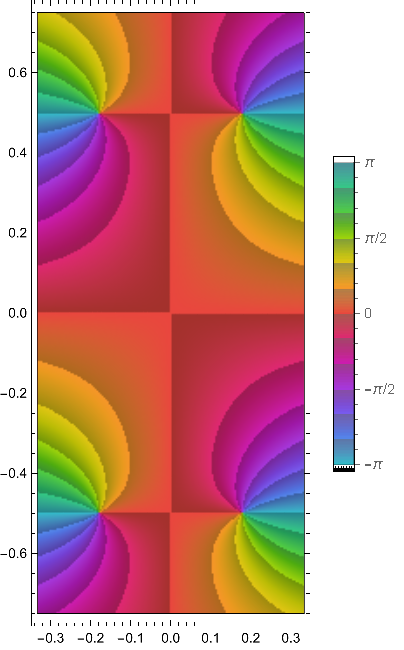
\includegraphics[width=1\linewidth]{images/delta_s2_plot_ordered.pdf}
        \label{fig:placeholder1}
        %\mathcal{A}ption{a}
    \end{subfigure}
    \begin{subfigure}{.3\textwidth}
        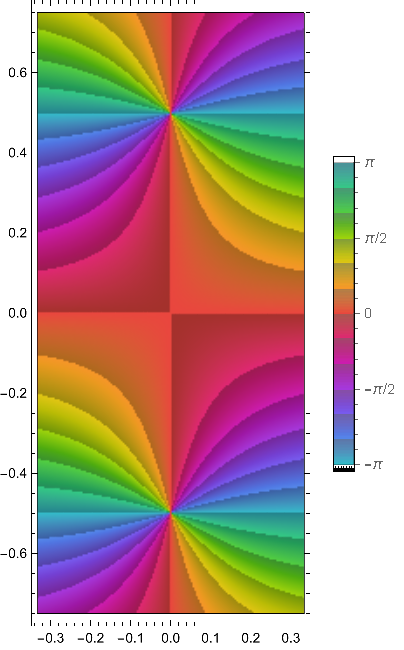
\includegraphics[width=1\linewidth]{images/delta_s2_plot_coincide.pdf}
        \label{fig:placeholder2}
        %\mathcal{A}ption{b}
    \end{subfigure}
    \begin{subfigure}{.3\textwidth}
        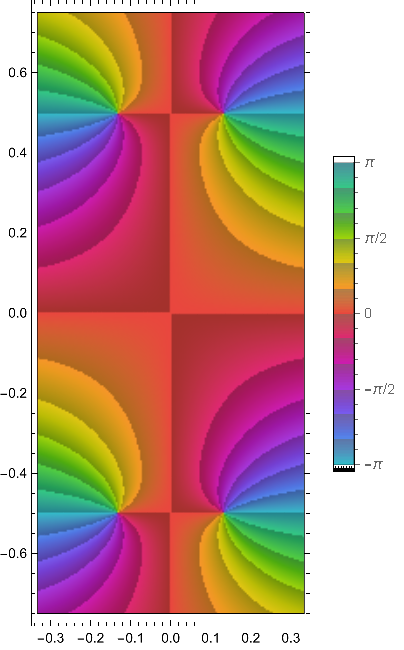
\includegraphics[width=1\linewidth]{images/delta_s2_plot_reversed.pdf}
        \label{fig:placeholder3}
        %\mathcal{A}ption{c}
    \end{subfigure}     
    \caption{The phase of $\Delta s^2$ as a function of $z$. The left figure is the case with $-\log(x_1- t_1+x_2- t_2) < \log(x_1+ t_1+x_2+ t_2)$. The middle one is the case with the branch points coinciding. The right one is the case with $-\log(x_1- t_1+x_2- t_2) > \log(x_1+ t_1+x_2+ t_2)$. To illustrate the results, we have picked $a = 1, x_1 = 0.1, t_1 = 0, t_2 = 0, 2h = 1.5$. The left one has $x_2 = 3$. The middle one has $x_1+x_2 = a$. The right one has $x_2 = 1/3$.}
    \label{fig:deltaS2_z}
\end{figure}

\begin{lemma} [Wedge-inside-wedge inclusion in CFT]
    For wedge-inside-wedge inclusion, the matrix element of the characteristic operator $f(z) = \bra{O(X)}\Delta_A^{1/2+iz}\Delta_B^{-iz}\ket{O(Y)}$, with self-adjoint scalar field $O(X), O(Y)$ and $Y\in B \subset A \ni X$, has the following properties:
    \begin{enumerate}
        \item There is an analytic continuation of $f(z)$ on the strip Im$(z)\in (-1/2,1/2)$. If the conformal dimension is not an integer, there are a pair of branch points on $\text{Im}(z)=\pm1/2$ each. If the conformal dimension is an integer, there are no branch cuts, and the branch points become poles.
        \item $f(z)$ is singular only when the transformed point-like field has zero proper distance.
        \item $f(z)$ has no zero. Zero is achieved only when the transformed point-like field has an infinite proper distance. The function decays exponentially to zero for large $|\text{Re}(z)|$.
        \item The function is real on Im$(z) = 0$, and therefore $f(\overline{z}) = \overline{f(z)}$.
        \item The function is real and continuous in the interval between the pair of singularities. If the pairs of singularities do not coincide, $f(z)$ can be extended to the whole complex plane, except for the singularities and possibly the branch cuts that repeat on $\text{Im}(z) \in \mathbb{Z} +1/2$. There is a choice of branch cuts where the function is periodic with period $i$, i.e. $f(z+i)=f(z)$. 
    \end{enumerate}
\end{lemma}

Although we only consider the point-like field $O(X),O(Y)$ in this setup, some features remain if we consider the smeared field. The smearing function may remove the singularities, but it cannot remove the branch cut. The multi-valued nature remains even with smeared fields. Also, several features remain valid in QFT and in higher dimensions. In general QFT, the two-point function of two self-adjoint point-like fields is still a function of the proper distance $\Delta s^2$. This is because the theory has Lorentz symmetry, and the modular flows of wedges remain geometric in QFT. The two-point function has a singularity only if $\Delta s^2 = 0$ in general. The function can only achieve zero with infinite proper distance. The function is real if the two points are spacelike separated at some $z$ due to causality. With these general features of QFT, most of the above properties and the singularity structure remain the same in general QFT, except for the details about the singularities and potentially the branch cuts. 

\subsection{Ball inside Wedge}
In this subsection, we consider the setup with ball-inside-wedge inclusion. There is a distinction compared to the case of a wedge inside a wedge. The wedge-inside-wedge inclusion has a common end point at infinity so that the inclusion is not split. The inclusion of a ball inside a ball is the same as the inclusion of a ball inside a wedge. There is a conformal transformation that maps the larger ball to a wedge. Without loss of generality, we consider the setup with a double cone $B$ included in the right Rindler wedge $A$ in 1+1d CFT. The modular flow of a double cone $B$ with the two tips $(t_c\pm r,x_c)$ is
\begin{align}
    \Delta_B^{-is} O(t,x) \Delta_B^{is} = \gamma^{2h} O(t_s,x_s),
\end{align}
where
\begin{gather}
    %t_s = \frac{2r^2(t-t_c) \cosh(2\pi s) + (r^2-d^2)r \sinh(2\pi s)}{r^2+d^2 + (r^2-d^2)\cosh(2\pi s) +2r(t-t_c)\sinh(2\pi s)} + t_c,\\
    t_s = \gamma \left[(t-t_c)\cosh(2\pi s) + \frac{r^2-d^2}{2r}\sinh(2\pi s)\right] + t_c,\\
    %x_s = \frac{2r^2(x-x_c)}{r^2+d^2 + (r^2-d^2)\cosh(2\pi s) +2r(t-t_c)\sinh(2\pi s)} + x_c,\\
    x_s = \gamma (x-x_c) + x_c,\\
    \gamma = \frac{2r^2}{r^2+d^2 + (r^2-d^2)\cosh(2\pi s) +2r(t-t_c)\sinh(2\pi s)}, \\
    d^2 = -(t-t_c)^2 + (x-x_c)^2.
\end{gather}
For $(t,x) \in B$ and $s\in \mathbb{R}$ , $\gamma>0$ and the point $(t_s,x_s)$ remains in $B$ . For $(t,x) \notin B$, $\gamma$ could be non-positive for some real $s$. This corresponds to the point-like field crossing infinity and reaching the other patch of Minkowski space. There will be a phase from $\gamma^{2h}$ when $2h$ is non-integer. For computing the matrix element of the characteristic operator, we only need the case where $(t,x) \in B$.

The matrix element of the characteristic operator depends on the proper distance and the conformal factor $\gamma$. We consider $f(z)=\bra{O(X)}\Delta_A^{1/2+iz}\Delta_B^{-iz}\ket{O(Y)}$ with $Y\in B \subset A\ni X$. For $X = (t_1,x_1), Y = (t_2+t_c,x_2+x_c)$, and real $z$, we have
\begin{gather}
    %\gamma &= \frac{2r^2}{r^2+d^2 + (r^2-d^2)\cosh(2\pi z) +2rt_2\sinh(2\pi z)} \\
    \gamma= \frac{4r^2 e^{2\pi z}}{r^2-d^2+2rt_2} \frac{1}{(e^{2\pi z} + p_+)(e^{2\pi z} + p_-)},\\
    %\Delta t &= -t_1 \cosh(2\pi z) - x_1 \sinh(2\pi z) - \gamma\left[t_2\cosh(2\pi z) + \frac{r^2-d^2}{2r}\sinh(2\pi z)\right] - t_c, \\
    %\Delta x &=   -t_1 \sinh(2\pi z) - x_1 \cosh(2\pi z) - \gamma x_2 - x_c,\\
    \Delta x + \Delta t = -(x_1+t_1)e^{2\pi z} - (x_c+t_c) - r\frac{e^{2\pi z}-p_-}{e^{2\pi z}+p_-},\\
    \Delta x - \Delta t = - (x_1-t_1)e^{-2\pi z} - (x_c-t_c) - r\frac{e^{2\pi z}-p_+}{e^{2\pi z}+p_+},\\
    %f(z) &= \gamma^{h} \frac{C}{[\Delta s^2-i\epsilon(t_1 \cosh(2\pi z) + x_1 \sinh(2\pi z) + \gamma (t_2\cosh(2\pi s) + \frac{r^2-d^2}{2r}\sinh(2\pi s))+t_c)]^{h}}.
    f(z) = C \left(\frac{\gamma}{-\Delta t^2 + \Delta x^2} \right)^{2h},
\end{gather}
where
\begin{gather}
    d^2 = -t_2^2 + x_2^2, \quad p_\pm = \frac{r^2+d^2\pm 2rx_2}{r^2-d^2+2rt_2} > 0,\\
    p_+p_- = \frac{r^2-d^2-2rt_2}{r^2-d^2+2rt_2}.
\end{gather}
We can then consider the analytic continuation of $f(z)$ with complex $z$. Similar to the previous case, the singularities are located at $\Delta s^2 = 0$. The above expression may suggest that $\gamma \to \infty$ is another possible singularity. However, $\gamma \to \infty$ is achieved only if the point $Y$ is mapped to the infinity. The infinite proper distance ensures that $f(z)$ is finite even if $\gamma$ diverges. For $\Delta s^2/\gamma = 0$, we have
\begin{gather}
    (x_1+t_1)e^{4\pi z} +  (x_c + t_c + r + p_-x_1+ p_-t_1)e^{2\pi z}+ (x_c+t_c-r) p_-  = 0,\\
    \text{or } \quad (x_1-t_1)e^{-4\pi z}+ \left(x_c - t_c - r+\frac{x_1-t_1}{p_+}\right)e^{-2\pi z} + \frac{x_c-t_c + r}{p_+} = 0.
\end{gather}

The general properties are summarized in the following lemma.
\begin{lemma} [Ball-inside-wedge inclusion in CFT]
    For ball-inside-wedge inclusion $B\subset A$, the matrix element of the characteristic operator $f(z) = \bra{O(X)}\Delta_A^{1/2+iz}\Delta_B^{-iz}\ket{O(Y)}$, with self-adjoint scalar field $O(X), O(Y)$ and $Y\in B \subset A \ni X$, has the following properties:
    \begin{enumerate}
        \item There is an analytic continuation of $f(z)$ on the strip Im$(z)\in (-1/2,1/2)$. If the conformal dimension is not an integer, there are two pairs of branch points on $\text{Im}(z)=\pm1/2$ each. If the conformal dimension is an integer, there are no branch cuts, and the branch points become poles.
        \item $f(z)$ is singular only when the transformed point-like fields have zero proper distance.
        \item $f(z)$ has no zero. Zero is achieved only when $|\text{Re}(z)| \to \infty$. The function decays exponentially to zero for large $|\text{Re}(z)|$.
        \item The function is real on Im$(z) = 0$, and therefore $f(\overline{z}) = \overline{f(z)}$.
        \item There is a interval between two singularities for which the function is real and continuous, if the singularities do not coincide. In that case, $f(z)$ can be extended to the whole complex plane, except for the singularities and possibly the branch cuts that repeat on $\text{Im}(z) \in \mathbb{Z} +1/2$. There is a choice of branch cuts where the function is periodic with period $i$, i.e. $f(z+i)=f(z)$. 
    \end{enumerate}
\end{lemma}
One main difference compared to the wedge-inside-wedge case is that there are more singularities and, in general, more branch cuts on $\text{Im}(z) = \pm 1/2$. In this case, $\Delta x \pm \Delta t = 0$ gives two quadratic equations of $e^{\pm 2\pi z}$. In the wedge-inside-wedge case, $\Delta x \pm \Delta t = 0$ gives a linear equation of $e^{\pm2\pi z}$. Another difference is that these properties are more restricted to CFT only. In a QFT, the modular flow of a ball-shaped region is not geometrical in general. We cannot directly carry the proper distance argument to QFT. Because of this limitation, we consider the approach of conformal perturbation method in the next section.

\NL{Study this in modular frequency space}

\subsection{Chaos Bound}
\KL{==========================Chaos bound===================}\\
We consider the modular chaos bound condition studied in \cite{}. We define
\begin{eqnarray}
    f_\mO(u)&&=\frac{\bra{\mO}\Delta_A^{1/2+iu}\Delta_B^{-iu}\ket{\mO}}{\sqrt{\braket{a|\Delta_A^{1/2}a}\braket{b|\Delta_B^{1/2}b}}}\\
    &&=\frac{\bra{\Delta_A^{1/4}\mO} T_{B\subset A}(-i/4+u)\ket{\Delta_B^{1/4} \mO}}{\sqrt{\braket{\mO|\Delta_A^{1/2}\mO}\braket{\mO|\Delta_B^{1/2}\mO}}}\nn\\
    &&=1+i \mathcal{M}_{\mO}(u)
\end{eqnarray}
First, we find that 
\begin{eqnarray}
    1-\Im(\mathcal{M}_\mO(u))=\Re(f_\mO(u))\leq |f_\mO(u)|\leq 1
\end{eqnarray}
which implies that 
\begin{eqnarray}
    \Im\mathcal{M}_\mO(u)\geq 0\ .
\end{eqnarray}
Using the change of variables $E=ie^{-2\pi u}$ sends the function above to the upper half-plane. Therefore, we can view $\mM(E)$ as an analytic map from the upper half-plane $H$ to itself. Then, writing $E=v+iw$ the Schwarz-Pick lemma becomes
\begin{eqnarray}
    \frac{|w \p_w \mM(v+iw)|}{\Im \mM(v+iw)}\leq 1\ . 
\end{eqnarray}
Since we have $|\p_w \Im\mM(v+i\omega)|\leq |\p_w \mM(v+i\omega)|$ we find
\begin{eqnarray}
    |w\p_w \log \Im \mM(v+iw)| \stackrel{(1)}{\leq} \frac{|w \p_w \mM(v+iw)|}{\Im \mM(v+iw)} \stackrel{(2)}{\leq} 1\ .
\end{eqnarray}
This is the modular chaos bound. To saturate this bound, first we need to take the equality condition $(2)$ in the lemma above, which fixes $\mM(E)=\frac{a E+b}{c E+d}$ to be a $PSL(2,\mathbb{R})$ transformation. Next, we require the saturation of the first inequality $(1)$
\begin{eqnarray}
    \forall v+iw\in H:\qquad \p_w \Re \mM(v+iw)=0\ .
\end{eqnarray}
This is satisfied if and only if $c=0$, i.e.
\begin{eqnarray}
    \mM(E)=\frac{a E+b}{d}\ .
\end{eqnarray}
\KL{*****} However, this inequality is not tight, i.e. $|w\p_w \log \Im \mM(v+iw)| < 1$. It is like a supremum rather than a maximum.
\begin{lemma}
    Consider a function $\mM(E)$ that is analytic in the upper half-plane ($\Im E > 0$). If it can be written as $f(E) = 1+i\mM(E)$ for some function $f(E)$ that is bounded by 1 in the upper half-plane, then the modular chaos bound cannot be saturated. In other words,
    \begin{align}
        |w\p_w \log \Im \mM(v+iw)| < 1.
    \end{align}
\end{lemma}
We can write $\mM = -i(f-1)$. The image of $\mM$ is within the unit disk centered at $i$ in $\mathbb{C}$. Inequality $(2)$ is saturated if and only if the function is a M\"obius transformation with real coefficients. These M\"obius transformations are bijetive functions mapping from the upper half-plane to itself. The image of $\mM$ is by definition a strict subset of the upper half-plane, whereas the domain is the entire upper half-plane. The inequality can never exactly saturate. Instead, we can look for an asymptotic saturation under suitable limits. The modular chaos bound is proposed as the following\cite{}. Consider $\mM = i\varepsilon p e^{\lambda u} + O(\varepsilon^2)$ for some small $\varepsilon \ll 1$, $\varepsilon e^{\lambda u} \ll 1$, and $p>0$. The above inequality gives $\lambda \leq 2\pi$. This is the modular chaos bound. This chaos bound is only meaningful in a proper range of time scales. 

We now consider a $0+1$d GFF example.

%\KL{======== 0+1d GFF ==================================}


\KL{=======================2. The Modular Chaos bound in GFF ============}\\
\KL{Not finished yet.}

\subsection{Modular chaos bound in GFF}

We then consider the modular chaos bound in the 0+1d GFF example. We consider $B = (-1,1)$ and $B(s) = (-e^{-2\pi s}, e^{-2\pi s})$. We define
\begin{eqnarray}
    f_{s,x}(u)&&=\frac{\bra{\phi(x)}\Delta_B^{1/2+iu}\Delta_{B(s)}^{-iu}\ket{\phi(x)}}{\sqrt{\braket{\phi(x)|\Delta_B^{1/2}\phi(x)}\braket{\phi(x)|\Delta_{B(s)}^{1/2}\phi(x)}}}\\
    &&=\frac{\bra{\Delta_A^{1/4}\phi(x)} T_{0,s}(-i/4+u)\ket{\Delta_B^{1/4} \phi(x)}}{\sqrt{\braket{\phi(x)|\Delta_B^{1/2}\phi(x)}\braket{\phi(x)|\Delta_{B(s)}^{1/2}\phi(x)}}}\nn\\
    &&=1+i \mathcal{M}_{s,x}(u),
\end{eqnarray}
for $x \in B(s)\subset B$. By substituting $E = ie^{-2\pi u} \in {\mathbb{H}_+}$ for $\Im u \in (-\pi/4,\pi/4)$, we have
\begin{align}
    the.long.complicated.expression.here.finish.it.later
\end{align}
This is not a M\"obius transformation, which is expected. In the $\pi s \ll 1$ limit, we have
\begin{align}
    f_{s,x}(E) &= 1 - i\pi s h\lb \frac{1-x}{1+x}\frac{1}{E} - \frac{1+x}{1-x}E \rb + O((\pi s)^2),\\
    f_{s,x}(u) &= 1 - \pi s h\lb \frac{1-x}{1+x}e^{2\pi u} + \frac{1+x}{1-x}e^{-2\pi u} \rb + O((\pi s)^2).
\end{align}
We then consider the late time behaviour in a double-scale limit, i.e. $e^{2\pi u} \gg1$ while keeping $1\gg\pi se^{2\pi u}$. The previous expression gives
\begin{align} 
    f_{s,x}(u) \approx 1 - \pi s h \frac{1-x}{1+x}e^{2\pi u},\\
    \mM_{s,x}(u)\approx i\pi s h \frac{x-1}{x+1}e^{2\pi u}.
\end{align}
This is the saturation of the modular chaos bound asymptotically. It gives a similar result if we consider $e^{-2\pi u} \gg1$ instead. In other words, $\mM_{s,x}(u) \sim ise^{2\pi |u|}$ for $e^{2\pi |u|} \gg 1\gg\pi se^{2\pi |u|}$.



\section{Subregion flows in Conformal Perturbation Theory}\label{section:conformalperturbation}


%\NL{should we call them geometric or local inclusions or not?}

4.1. Setup of perturbation of modular flow, 4.2. cocycle flow, 4.3. 1st order correction of characteristic function, 4.4 analytic property 

A short paragraph about general QFT, move on to conformal perturbation theory, %mention that only 2- and 3-pt functions are universal, best is first order correction if without CFT details 
\subsection{Modular Flow with Conformal Perturbation Method}

\NL{Without loss of generality and for simplicity of presentation for the remainder of this section, we focus on 1+1 D QFT}

To study the characteristic function in QFT,  we first compute the modular flow perturbatively. We apply the conformal perturbation method to compute the modular flow of a ball-shaped region. We follow the method in \cite{,} and consider the Lagrangian perturbed with a relevant deformation 
\begin{align}
    \mathcal{L}_\text{CFT} \to \mathcal{L}_\text{CFT} - \lambda O(x), 
\end{align}
where $O(x)$ is a conformal primary in the flat space coordinate $x$ and $\lambda$ is a small parameter. The modular flow $e^{isK_\lambda}$ of an algebra $\mathcal{A}$ associated to a ball-shaped region $I$ (restricted to the algebra) can be computed perturbatively
\begin{gather}
    \delta_\lambda(e^{isK_\lambda}) = \int_0^1 dw e^{iswK_0} is\delta_\lambda K_\lambda e^{is(1-w)K_0} , \\
    \delta_\lambda K_\lambda= \int_{-\infty + i\theta}^{\infty + i\theta} \frac{2\pi du}{4\sinh^2(\pi u)} e^{iuK_0}\rho^{-1}\delta\rho e^{-iuK_0}, \quad\text{for } 0<\theta<1,\\
    \rho^{-1}\delta\rho = -\lambda\int_I d^{D-1}X\int_0^1 d\tau J(\tau,X) \Omega^{\Delta}(-i\tau,X) e^{\tau K_0} O(X) e^{-\tau K_0} ,
\end{gather}
where $J$ is the Jacobian determinant between the geometrically transformed coordinate  on $e^{\tau K_0} O(X) e^{-\tau K_0}$ and $(X, \tau)$, $\Omega$ is the conformal factor that depends on the geometric action of the flow $e^{is K_0}$, $\Delta$ is the conformal dimension of $O$\footnote{We would consider $D/2 < \Delta < D$ for the perturbation method to work \cite{}.}, and $D$ is the spacetime dimension. $K_\lambda$ here is not the full modular Hamiltonian. It is the one-sided modular Hamiltonian that acts only on the algebra. By substituting $\rho^{-1}\delta_\lambda\rho$ into the expression of $\delta_\lambda K_\lambda$ and changing the order of integration, we can choose $\theta = \tau$ to cancel the Euclidean part and obtain a  purely Lorentzian action \cite{}
\begin{align}
    \delta_\lambda K_\lambda=& -\lambda\int_I dX\int_0^1 d\tau \int_{-\infty}^{\infty} du \, \frac{2\pi J(\tau,X)}{4\sinh^2(\pi (u+i\tau))}   \Omega^{\Delta}(-i\tau,X) e^{iuK_0} O(X) e^{-iuK_0} \\
    =& \pi \lambda\int_I dX \int_{-\infty}^{\infty} du \, h(u,X) e^{iuK_0} O(X) e^{-iuK_0}, \label{eq:deltaK}
\end{align}
where we define
\begin{align}
    h(u,X) \equiv -\int_0^1\, d\tau \frac{J(\tau,X)\Omega^{\Delta}(-i\tau,X)}{2\sinh^2(\pi (u+i\tau))} 
\end{align}
Without loss of generality and for simplicity of the presentation, we focus on 1+1 D QFT. For simplicity, we consider $I$ to be the interval $(-1,1)$ at $t = 0$. The unit ball $B$ is the double cone corresponding to $I$. We can obtain the result for a double cone in general position by applying the Lorentz transformation on the unit ball $B$. We can put $r$ back for ball-shaped region with radius $r$. We can also generalize the result to ball-shaped regions in higher dimension. %In this setup, we have 
% \begin{gather}
%     e^{isK_0} O(t,x) e^{-isK_0} = \tilde{\Omega}^{-\Delta} O(t_s,x_s), \\
%     \tilde{t}_s = \tilde{\Omega}^{-1}\left[t \cosh(2\pi s) + \frac{(1+t^2-x^2)}{2}\sinh(2\pi s) \right],\\
%     \tilde{x}_s = \tilde{\Omega}^{-1}x, \\
%    \tilde {\Omega}^{-1} = \frac{2}{1-t^2+x^2+(1+t^2-x^2)\cosh(2\pi s) + 2t \sinh(2\pi s)}.
% \end{gather}
In this set up, for $O(t=0,x)$, we have
\begin{gather}
    e^{isK_0} O(t,x) e^{-isK_0} = \Omega^{-\Delta} O(t_s,x_s), \\
    t_s = {\Omega}^{-1}\left[\frac{(1-x^2)}{2}\sinh(2\pi s) \right], \quad x_s = {\Omega}^{-1}x, \\
    {\Omega}(s,x) =  \frac{1+x^2+(1-x^2)\cosh(2\pi s)}{2} = 1+(1-x^2)\sinh^2(\pi s).
    %{\Omega}(s,x) = \tilde{\Omega}|_{t=0}= \frac{1+x^2+(1-x^2)\cosh(2\pi s)}{2} = 1+(1-x^2)\sinh^2(\pi s).
\end{gather}
The conformal factor $\Omega$ is $\gamma^{-1}$ in previous section with $r = 1, t =t_c=x_c=0$. The conformal factor $\Omega$ and the Jacobian determinant $J$ in Euclidean evolution are
\begin{gather}
    \Omega(-i\tau,x)= \frac{1+x^2+(1-x^2)\cos(2\pi \tau)}{2} =1-(1-x^2)\sin^2(\pi \tau),\\
    J(\tau,x) = \det \left.\begin{pmatrix}
        \partial_st_{s} & \partial_s x_{s}\\  \partial_X t_{s}& \partial_X x_{s}
    \end{pmatrix}\right|_{s=-i\tau} =\frac{\pi (1-x^2)}{\Omega(\tau,x)^2},\\
    \implies h(u,X) = -\pi(1-X^2)\int_0^1\, d\tau \frac{\Omega^{\Delta-2}(-i\tau,X)}{2\sinh^2(\pi (u+i\tau))}.
\end{gather}
%{(Maybe write it as something like convolution, and the delta function like fattened, also try numeric/plot to see. Also see $x^2=1$ is special, maybe like interpolation between x, or some coarse graining)}
Notice that the $d\tau$ integral of $h(u,X)$ can be done explicitly if there is no $\Omega^{\Delta-2}(-i\tau,X)$, with
\begin{align}
    -\int_0^1\, \frac{ \pi d\tau }{2\sinh^2(\pi (u+i\tau))} = \delta(u).
\end{align}
A similar calculation appears in the calculation for the Rindler wedge case. The modular flow of the Rindler wedge in a CFT is a boost, which gives a trivial conformal factor. This delta function combined with the CFT modular Hamiltonian gives the new boost operator in the QFT \cite{}. With the delta function, Eq. (\ref{eq:deltaK}) becomes an integral of $X$ only. This term is the local contribution.  If $\Delta = 2$, the extra factor $\Omega^{\Delta-2}(-i\tau,X)$ becomes trivial and we obtain the delta function as in the Rindler wedge case. The intuition is that the modular flow remains geometric because the deformed CFT is just another CFT, though $\Delta = 2$ is a marginal perturbation and this may not be a suitable application of the perturbation method. For these reasons, we separate the divergent part from the integral
\begin{gather}
    h(u,X) =  (1-X^2)\left[\delta(u) + h_{reg}(u,X)\right], \\
    h_{reg}(u,X) \equiv -\pi\int_0^1\, d\tau \frac{ (\Omega^{\Delta-2}(-i\tau,X) -1)}{2\sinh^2(\pi (u+i\tau))} .
\end{gather}
By combining all the expressions, we have
\begin{align}
    u_{s,\lambda} =&\; e^{-isK_0}e^{isK_\lambda} \approx 1 + e^{-isK_0}\delta e^{isK_\lambda}\\
    =&\; 1 + i\pi s\lambda\int_0^1 dw  \int_{-1}^1 dX \int_{-\infty}^{\infty} du \, h(u,X) e^{i(u+sw-s)K_0} O(X) e^{-i(u+sw-s)K_0} \\
    =&\; 1 + i\pi \lambda\int_0^s dw  \int_{-1}^1 dX \int_{-\infty}^{\infty} du \, h(u+w,X) e^{iuK_0} O(X) e^{-iuK_0} \\
    =&\; 1 + i\pi \lambda\int_0^s dw  \int_{-1}^1 dX \int_{-\infty}^{\infty} du \, (1-X^2)\left[\delta(u+w) + h_{reg}(u+w,X)\right] e^{iuK_0} O(X) e^{-iuK_0}\\
    =&\; 1 + i\pi \lambda\int_{-s}^0 dw  \int_{-1}^1 dX \, (1-X^2)e^{iwK_0} O(X) e^{-iwK_0} \nonumber\\
    &+ {i\pi \lambda}\int_0^s dw  \int_{-1}^1 dX \int_{-\infty}^{\infty} du \, (1-X^2)h_{reg}(u+s,X) \Omega^{-\Delta}(u,X)O(t_u,x_u).
\end{align}
Thus, we have
\begin{gather}
    u_{s,\lambda} = 1 + i\pi \lambda \int_{-1}^1 dX \int_{-\infty}^{\infty} du \, (1-X^2) Q(u,X;s) \Omega^{-\Delta}(u,X) O(t_u,x_u) +O(\lambda^2),\\
    Q(u,X;s) = Q_{\text{loc}}(u,X;s) + Q_{\text{nonloc}}(u,X;s),\\
    Q_{\text{loc}}(u,X;s) =  \textbf{1}_{(-s,0)}(u),
\end{gather}
and 
\begin{align}
    Q_{\text{nonloc}}(u,X;s) \equiv&\;\int_0^s dw \; h_{reg}(u+w,X) \nonumber\\
    =&\; -\pi\int_0^s dw\int_0^1 \, d\tau  \;\frac{\left(1 - (1-X^2)\sin^2(\pi \tau)\right)^{\Delta-2} -1}{2\sinh^2(\pi (u+w+i\tau))}.
\end{align}
%{(Emphasis the local, non local, emphasis the role of $w, x, u$, rewrite the first term to look more local, combine $sdw$, maybe even bring the range $\int_0^s$ to the $1_{[-s,0]}$, bring the local term here, etc.)} 
$\textbf{1}_{(-s,0)}(x)$ is the indicator function of $(-s,0)$\footnote{If $s < 0$, we set $\textbf{1}_{(-s,0)}(x) = - \textbf{1}_{(0,-s)}(x)$.}. $Q_{\text{loc}}$ is the contribution of the delta function, which is the local contribution term to the correction of the modular Hamiltonian. $Q(u,X;s)$ should be interpreted in terms of distribution. If $\Delta > 3/2$, we can swap the order of the integral of $dw$ and $d\tau$. The divergences at $u = 0, \tau = 0 , 1$ are regulated by separating $Q_{\text{loc}}$. The divergence at $X=0, \tau = 1/2$ is mild enough so that the integrand is absolutely integrable. This allows us to change the order of integration. 
\begin{align}
    Q_{\text{nonloc}}(u,X;s) =&\; \int_0^1 \, d\tau \; \left[\left(1 - (1-X^2)\sin^2(\pi \tau)\right)^{\Delta-2} -1\right] \nonumber\\
    &\times\frac{\coth(\pi(u+s+i\tau)) - \coth(\pi(u+i\tau))}{2}.
\end{align}
The integral of $X$ and $u$ is the integration over the double cone region. The $Q_{\text{loc}}$ term is simply a indicator function. The contribution is the local perturbation from zero modular evolution to $-s$. The $Q_{\text{nonloc}}$ term has an extra integral of the Euclidean modular time $\tau$. Although the result is purely Lorentzian, the Euclidean modular evolution contributes to the weight function. For general $\Delta-2 < 0$, the integral is hard to compute.
%\KL{(play around $s,w,u$ to see if symmetrize the expression, maybe write the $s$ as some indicator function)}


\paragraph{Almost-marginal relevant operators*:} 
We consider small $\epsilon =2-\Delta\ll 1$ and expand $Q_{\text{nonloc}}(u,X;s)$ up to the leading order term. We have the following expansion\footnote{One may worry that the first order approximation is only valid for $\epsilon \ln\Omega \ll 1$ but $\Omega$ can be arbitrarily large when $X\approx 0$ and $\tau \approx 1/2$. We can split the $\tau$ integral into $(\frac{1}{2}-\delta, \frac{1}{2}+\delta)$ and the rest, with $1 \gg \pi\delta > e^{-\frac{1}{2\epsilon}}$. For $X\approx0$, $\Omega^{\Delta-2} \approx (X^2+\pi^2\delta^2)^{\Delta-2}$ such that the integral in $(\frac{1}{2}-\delta, \frac{1}{2}+\delta)$ is $O(e^{-\frac{1}{2\epsilon}})$. The width of the interval is also $O(e^{-\frac{1}{2\epsilon}})$. This is also how we see the integrand of $Q_{\text{nonloc}}$ being absolutely integrable for $\Delta > 3/2$. The orthogonality of cosine functions we use later also remains approximately true because of the same reason.}
\begin{align}
    \Omega^{\Delta-2}(-i\tau,X) - 1 =&\; - \epsilon \ln \left(\frac{1+X^2+(1-X^2)\cos(2\pi \tau)}{2}\right) + O(\epsilon^2)\\
    =&\; - \epsilon \ln \left[\frac{1+X^2}{2}\left(1+\frac{1-X^2}{1+X^2}\cos(2\pi \tau)\right)\right] + O(\epsilon^2). %\\
    %= &\; \epsilon \sum_{n=0}^{\infty} \left( \right)\cos(2 \pi n \tau) + O(\epsilon^2) 
\end{align}
% We use the identity ($r\in (-1,1), \tau\in[0,1]$)
% \begin{align}
%     \ln(1+r^2 + 2r\cos(2\pi\tau)) =&\; \ln(1+re^{i2\pi\tau}) + \ln (1+re^{-i2\pi\tau})\\
%     =&\; -\sum_{n= 1}^{\infty} \frac{(-r)^n e^{i2\pi n\tau}}{n} -\sum_{n= 1}^{\infty} \frac{(-r)^n e^{-i2\pi n\tau}}{n} \\
%     =&\; -\sum_{n \neq 0} \frac{(-r)^{|n|}e^{i2\pi n\tau}}{|n|} .
% \end{align}
We can expand $\Omega^{\Delta-2}(-i\tau,X)$ as a Fourier series $\Omega^{\Delta-2}(-i\tau,X) = \sum_{n} a_n e^{i2\pi n \tau}.$ We have\footnote{We use the identity $\ln(1+r^2 + 2r\cos(2\pi\tau)) = \ln\left[(1+re^{i2\pi\tau})(1+re^{-i2\pi\tau})\right] = -\sum_{n \neq 0} \frac{1}{|n|}(-r)^{|n|}e^{i2\pi n\tau}$ for $r\in (-1,1), \tau\in[0,1]$ and substituting $r = \frac{1-|X|}{1+|X|}$.}
\begin{gather}
    \Omega^{\Delta-2}(-i\tau,X) - 1 = \epsilon \left(\sum_{n} a_n^{(1)}e^{i2 \pi n \tau} \right) + O(\epsilon^2),\\
    a_0^{(1)} =  -2\ln \frac{1+|X|}{2}, \quad a_{n \neq 0}^{(1)} = \frac{1}{|n|} \left(-\frac{1-|X|}{1+|X|}\right)^{|n|}.
\end{gather}
We can also expand the $\coth$ function as
\begin{align}
    \coth(\pi (u+i\tau)) =& \frac{e^{\pi (u+i\tau)}+e^{-\pi (u+i\tau)}}{e^{\pi (u+i\tau)}-e^{-\pi (u+i\tau)}} \nonumber\\
    % =& \begin{cases}
    %     (1+e^{-2\pi (u+i\tau)}) \sum_{m=0}^{\infty} e^{-2\pi m (u+i\tau)}, & \text{for } u > 0,\\
    %     -(1+e^{2\pi (u+i\tau)}) \sum_{m=0}^{\infty} e^{2\pi m (u+i\tau)}, & \text{for } u < 0,
    % \end{cases}\\
    =& \begin{cases}
        1+\sum_{m=1}^{\infty} 2e^{-2\pi m (u+i\tau)}, & \text{for } u > 0,\\
        -(1+\sum_{m=1}^{\infty} 2e^{2\pi m (u+i\tau)}), & \text{for } u < 0,
    \end{cases}\\
    =& \;\text{sign}(u) \left(1+ \sum_{m \neq 0 } \theta_{\text{step}}(-mu)2 e^{2\pi m u} e^{i2\pi m \tau}\right)
\end{align}
Thus, we have
\begin{align}
    &\int_0^1 \, d\tau \; \left[\Omega^{\Delta-2}(-i\tau,X) -1\right] \coth(\pi(u+i\tau)) \nonumber\\
    =&\; \text{sign}(u)2\epsilon\left[-\ln\frac{1+|X|}{2}+\sum_{n\neq0} \theta_{\text{step}}(nu) e^{-2\pi n u} \frac{1}{|n|}\left(-\frac{1-|X|}{1+|X|}\right)^{|n|} \right] +O(\epsilon^2)\\
    =&\; -\text{sign}(u)2\epsilon \ln\left(\frac{1+|X| +(1-|X|)e^{-2\pi|u|}}{2}\right) +O(\epsilon^2).
\end{align}
The integral becomes
\begin{align}
    Q_{\text{nonloc}}(u,X;s) =&\; Q^{(1)}_{\text{nonloc}}(u,X) + O(\epsilon^2)\\
    Q^{(1)}_{\text{nonloc}}(u,X;s) =&\; -\epsilon\left\{ \text{sign}(u+s)\ln\left(\frac{1+|X| +(1-|X|)e^{-2\pi|u+s|}}{2}\right) \right. \nonumber\\
    & \left.- \text{sign}(u)\ln\left(\frac{1+|X| +(1-|X|)e^{-2\pi|u|}}{2}\right) \right\}.
\end{align}
When we evaluate the integral of $u$, we can break it into $\int_{-\infty}^{\text{min}(-s,0)}$, $\int_{\text{min}(-s,0)}^{\text{max}(-s,0)}$, and $\int_{\text{max}(-s,0)}^{\infty}$. For $u<\text{min}(-s,0)$, 
\begin{gather}
    Q_{\text{nonloc}}(u,X;s) = \epsilon\ln\left( \frac{1+|X| +(1-|X|)e^{2\pi(u+s)}}{1+|X| +(1-|X|)e^{2\pi u}}\right)
\end{gather}
For $\text{max}(-s,0)<u$,
\begin{align}    
    Q_{\text{nonloc}}(u,X;s) &= \epsilon\ln\left( \frac{1+|X| +(1-|X|)e^{-2\pi u}}{1+|X| +(1-|X|)e^{-2\pi(u+s)}}\right) \\
    &= \epsilon\ln\left( \frac{1-|X| + (1+|X|)e^{2\pi u} }{1-|X| + (1+|X|)e^{2\pi(u+s)} }\right) +\epsilon2\pi s.
\end{align}
For $\text{min}(-s,0)<u<\text{max}(-s,0)$, we have
\begin{align}
    \text{sign}(-s)\epsilon\ln\left(({1+|X| +(1-|X|)e^{-2\pi|u+s|}})({1+|X| +(1-|X|)e^{-2\pi|u|}})\right).
\end{align}
Notice that $Q^{(1)}_{\text{loc}}(u,X;s)$ has support only for $\text{min}(-s,0)<u<\text{max}(-s,0)$.
%{(See if the symmetrization helps to rewrite the log - log function)}
% Thus, the cocycle is 
% \begin{align}
%     u_{s,\lambda}=&\; 1 + i\pi s\lambda\int_0^1 dw  \int_{-1}^1 dX \, (1-X^2)e^{-iswK_0} O(X) e^{iswK_0} \nonumber\\
%     &+ i\pi s\lambda\int_0^1 dw  \int_{-1}^1 dX \int_{-\infty}^{\infty} du \, h_{reg}(u+sw,X) \Omega^{-\Delta}(u,X)O(t_u,x_u)\\
%     =&\; 1 + i\pi s\lambda \int_{-1}^1 dX \int_{-\infty}^{\infty} du \, Q(u,X) \Omega^{-\Delta}(u,X) O(t_u,x_u) +O(\lambda^2),
% \end{align}
% where 
% \begin{gather}
%     Q(u,X) =\; Q_{\text{nonloc}}(u,X) + Q_{\text{loc}}(u,X), \\
%     Q_{\text{loc}}(u,X) \equiv \; (1-X^2)\frac{1}{s} \textbf{1}_{(-s,0)}(u),
% \end{gather}
% and $\textbf{1}_{A}(x)$ is the indicator function of $A$. In the case where the perturbed QFT is another CFT ($\Delta = 2$), the non-local term $Q_{\text{nonloc}}$ vanishes. The local term $Q_\text{loc}$ combined with the original modular Hamiltonian gives the same geometric flow in the new CFT. 
To summarize the result, we have the following lemma.
\begin{lemma} [Perturbed Modular Flow of the Unit Ball]
    In 1+1D QFT with Lagrangian
    \begin{align}
        \mathcal{L}_\text{QFT} = \mathcal{L}_\text{CFT} - \lambda O(x),  
    \end{align}
    the modular flow (restricted to the algebra) of the unit ball centered at the origin is:
    \begin{gather}
        e^{is K_\lambda } = e^{is K_0} \left(1 + i\pi \lambda \int_{-1}^1 dX \int_{-\infty}^{\infty} du \, (1-X^2) Q(u,X;s) \Omega^{-\Delta}(u,X) O(t_u,x_u) +O(\lambda^2)\right),
    \end{gather}
    where
    \begin{gather}
        Q(u,X;s) =\; Q_{\text{loc}}(u,X;s) + Q_{\text{nonloc}}(u,X;s), \quad Q_{\text{loc}}(u,X) = \textbf{1}_{(-s,0)}(u),
    \end{gather}
    and 
    \begin{align}
        Q_{\text{nonloc}}(u,X;s) =\; -\pi\int_0^s dw\int_0^1 \, d\tau  \;\frac{\left(1 - (1-X^2)\sin^2(\pi \tau)\right)^{\Delta-2} -1}{2\sinh^2(\pi (u+w+i\tau))}
    \end{align}
    For $3/2<\Delta <2$, we have
    \begin{align}
        Q_{\text{nonloc}}(u,X;s) =&\; \int_0^1 \, d\tau \; \left[\left(1 - (1-X^2)\sin^2(\pi \tau)\right)^{\Delta-2} -1\right] \nonumber\\
        &\times\frac{\coth(\pi(u+s+i\tau)) - \coth(\pi(u+i\tau))}{2}.
    \end{align}
    For almost-marginal relevant operators with small $\ep = 2- \Delta \ll 1$, we have
    \begin{align}
        Q_{\text{nonloc}}(u,X;s) =&\; Q^{(1)}_{\text{nonloc}}(u,X) + O(\epsilon^2)\\
        Q^{(1)}_{\text{nonloc}}(u,X;s) =&\; -\epsilon\left\{ \text{sign}(u+s)\ln\left(\frac{1+|X| +(1-|X|)e^{-2\pi|u+s|}}{2}\right) \right. \nonumber\\
        & \left.- \text{sign}(u)\ln\left(\frac{1+|X| +(1-|X|)e^{-2\pi|u|}}{2}\right) \right\}.
    \end{align}
\end{lemma}
%\KL{(Pull the $1-X^2$, the $\frac{1+|X| +(1-|X|)e^{...}}{1+|X| +...}$ take a familiar form like modular flow, push the $s$ inside $w$? or somewhere. It is like 4 regims of the sign(u), sign(u+s), like the adding two modular flow, and how the vector field align)}

% ========== DON'T USE THE REST HERE ===========

% The action of the modular flow is
% \begin{align}
%     &e^{-isK_0}e^{isK_\lambda} \phi(t,x) e^{-isK_\lambda}e^{isK_0} \nonumber\\
%     \approx& \, \phi(t,x) + e^{-isK_0}\left[\delta_\lambda(e^{isK_\lambda}) \phi(t,x)e^{-isK_0} + e^{isK_0}\phi(t,x) \delta_\lambda(e^{-isK_\lambda}) \right]e^{isK_0},\\
%     %=& \, \phi(t,x) + e^{-isK_0}\left[\int_0^1 dw e^{iswK_0} is\delta_\lambda K_\lambda e^{-iswK_0} e^{isK_0}\phi(t,x)e^{-isK_0} - e^{isK_0}\phi(t,x)e^{-isK_0} \int_0^1 dw e^{is(1-w)K_0} is\delta_\lambda K_\lambda e^{-is(1-w)K_0} \right]e^{isK_0},\\
%     =& \, \phi(t,x) + is\int_0^1 dw \left[e^{-iswK_0} \delta_\lambda K_\lambda e^{iswK_0} ,\phi(t,x)\right], \\
%     =& \, \phi(t,x) + i\pi^2 \lambda s \int_0^1 dw\int_{-1}^1 dX \int_{-\infty}^{\infty} du  \,h(u+sw,X)\left[  e^{iuK_0} O(t=0,x=X) e^{-iuK_0} ,\phi(t,x)\right],\\
%     =& \, \phi(t,x) + i\pi^2 \lambda s \int_0^1 dw\int_{-1}^1 dX \int_{-\infty}^{\infty} du  \,h(u+sw,X) \Omega^{\Delta}(u,X) \left[ O(t_u,x_u) ,\phi(t,x)\right],\\
%     %=& \, \phi(t,x) + i\pi^2 \lambda s \int_{-1}^1 dX \int_{-\infty}^{\infty} du \, \tilde{h}(u,X;s)\left[  e^{iuK_0} O(0,X) e^{-iuK_0} ,\phi(t,x)\right],.
% \end{align}
% We recall the expression of $h(u+sw,X)$. We can perform the $\tau$-integral if $\Delta = 2$
% \begin{align}
%     \tilde{h}(u,X;s)=& \, \int_0^1 dw\, h(u+sw,X),\\
%     =& \, \int_0^1 dw\int_0^1 d\tau \, \frac{\pi^2}{\sinh^2(\pi (u+sw+i\tau))} \Omega^{\Delta - D}(\tau,X), \\
%     =& \, \int_0^1 d\tau \, \frac{1}{s}\Omega^{\Delta - D}(\tau,X) \left[ \coth(\pi (u+s+i\tau)) - \coth(\pi (u+i\tau))\right].
% \end{align}

% We estimate the difference between the two flows by
% \begin{align}
%     \lVert(e^{isK_\lambda} - e^{isK_0}) A\Omega_\lambda \rVert^2 = \lVert(e^{-isK_0}e^{isK_\lambda} - 1) A\Omega_\lambda \rVert^2 = 2 \text{Re}\braket{\Omega_\lambda|A(1-u_{s,\lambda})A|\Omega_\lambda},
% \end{align}
% where $A=A^\dagger \in \mathcal{A}$, $u_{s,\lambda} = e^{-isK_0}e^{isK_\lambda} \approx 1 + e^{-isK_0}\delta e^{isK_\lambda}$, and $\Omega_\lambda$ is the cyclic and separating QFT vacuum vector. In the first order perturbation, we have
% \begin{align}
%     u_{s,\lambda} &\approx 1 + is\lambda\pi^2 \int_{-1}^1 dx \int_{-\infty}^{\infty} du \left[\int_0^1 dw \, h(u+s-sw,X)\right] e^{iuK_0} O(0,x)  e^{-iuK_0}\\
%     &=1+ is\lambda\pi^2 \int_{-1}^1 dx \int_{-\infty}^{\infty} du \left[\int_0^1 dw \, h(u+s-sw,X) \tilde{\Omega}^{-\Delta}(u,x) \right] O(t_u,x_u) .
% \end{align}
% We then consider the case where $A = \int_{B}dX f(X) O(X)$, $\lVert(e^{isK_\lambda} - e^{isK_0}) A\Omega_\lambda \rVert^2$ becomes a 3-point function \KL{(The is also wrong, the leading order is a 4 pt function agian. The reason is that the Re will kill this term as it is purely imaginary)}
% \begin{align}
%     &\lVert(e^{isK_\lambda} - e^{isK_0}) A\Omega_\lambda \rVert^2\\ 
%     \approx&  -2 \text{Re } is\lambda\pi^2 \int_{B}dX_1\int_{B}dX_2\int_{-1}^1 dx \int_{-\infty}^{\infty} du \left[\int_0^1 dw \, h(u+s-sw,x) \tilde{\Omega}^{-\Delta}(u,x) f(X_1)f(X_2) \right] \nonumber\\
%     &\times \braket{\Omega_0|O(X_1) O(t_u,x_u) O(X_2)|\Omega_0}
% \end{align}

% \KL{Comment: Maybe should use $\Omega_0$ instead so that we can compute the 2/3-pt function.}

% Another quantity to estimate the difference is
% \begin{align}
%     &\lVert(e^{isK_\lambda}Ae^{-isK_\lambda} - e^{isK_0} A e^{-isK_0})\Omega_0 \rVert^2 \\
%     =&\, \lVert [A, u_{s,\lambda}^\dagger]\Omega_0 \rVert^2 \\
%     =&\, \braket{\Omega_0|A^2|\Omega_0} + \braket{\Omega_0|u_{s,\lambda} A^2 u_{s,\lambda}^\dagger|\Omega_0} - 2\text{Re }\braket{\Omega_0|A u_{s,\lambda} A u_{s,\lambda}^\dagger|\Omega_0}\\
%     \to &\braket{\Omega_0|[A^2, \lambda\delta u^\dagger]|\Omega_0} - 2\text{Re }\braket{\Omega_0|A[A, \lambda \delta u^\dagger]|\Omega_0}
% \end{align}
% \KL{The leading order} \KL{(The is also wrong, the leading order is a 4 pt function agian. The reason is that the Re will kill this term as it is purely imaginary)}
% Although they are 4-point functions, the first-order corrections are still 3-point functions, the same as the previous quantity. Since we are computing a commutator between $A$ and $u_{s,\lambda}^\dagger$, we can project out the spacelike separating part of $u_{s,\lambda}^\dagger$ relative to $A$. 

% \KL{Reminder: Check the order of integration issue, compare with the previous paper/interactive picture calculation, do the small s expansion first/order of scales, etc.}

% \KL{The leading order term of norm should be in $O(\lambda)$, thus the norm square is $O(\lambda^2)$. With two $A$ operators, the two power of $\lambda$ require two $O$ insertion, which results a 4-pt function in general.}

% \KL{=============== END =====================}



\subsection{First order Correction of Characteristic Operator}
With the perturbed modular flow, we can compute the characteristic operator with the conformal perturbation method. We compute $f(z)= \;_\lambda\bra{O_1(x)}\Delta_{A,\lambda}^{1/2+iz}\Delta_{B,\lambda}^{-iz}\ket{O_2(y)}_\lambda$ in a QFT parametrized by $\lambda$. If both $A$ and $B$ are wedge, the same result follows from the CFT case because the modular flows remain a boost. We consider the inclusion $B\subset A$, where $B$ is a unit double cone centered at the origin and $A$ is the wedge with the end point $(0,-x_w)$, $x_w >0$. We have a similar setup where $Y\in B$, $X\in A$, and $O=O^\dagger$. The von Neumann algebras associated to the same region but with different $\lambda$ are in general different. We assume that the operators remain in both the original algebras in the CFT and the new algebras of the QFT. We denote the primary operator of the perturbation to be $O_0$. We expand the function perturbatively as
\begin{align}
    f_\lambda(z) =&\;_\lambda\bra{O_1(x)}\Delta_{A,\lambda}^{1/2+iz}\Delta_{B,\lambda}^{-iz}\ket{O_2(y)}_\lambda \\
    =&\; _0\bra{O_1(x)}\Delta_{A,0}^{1/2+iz}\Delta_{B,0}^{-iz}\ket{O_2(y)}_0 + \lambda f^{(1)}(z) + O(\lambda^2).
\end{align}
There are three contributions to the first order correction. We have
\begin{gather}
    u_{s,\lambda} = e^{-isK_0}e^{isK_\lambda} = 1 + \lambda u_{s}^{(1)} +O(\lambda^2),\\
    u_{s}^{(1)} = i\pi  \int_{-1}^1 dX \int_{-\infty}^{\infty} du \, (1-X^2) Q(u,X;s) \Omega^{-\Delta}(u,X) O_0(t_u,x_u)\\
    \ket{\Omega_\lambda} = \ket{\Omega_0} + \lambda\ket{\Omega^{(1)}} + O(\lambda^2),\\
    \ket{\Omega^{(1)}} = \int_\mathbb{R} dX \int_{-\infty}^{0} d\tau O_0(-i\tau,X) \ket{\Omega_0}.
\end{gather}
We can rewrite $f_\lambda(z)$ in terms of $u_{s,\lambda}$ and $\Omega_\lambda$. We have
\begin{align}
    f_\lambda(z) =&\;_\lambda\bra{O(x)}\Delta_{A,\lambda}^{1/2+iz}\Delta_{B,\lambda}^{-iz}\ket{O(y)}_\lambda \\
    =&\;\bra{\Omega_\lambda}O(x) \Delta_{A,\lambda}^{1/2+iz}\Delta_{B,\lambda}^{-iz}O(y) \ket{\Omega_\lambda}\\
    =& \; \bra{ \Omega_\lambda} \alpha_{A}^{-z}\left(O(x_J)\right) \left( \Delta_{B,0}^{-iz}\Delta_{B,0}^{+iz} \Delta_{B,\lambda}^{-iz}O(y) \Delta_{B,\lambda}^{+iz}\Delta_{B,0}^{-iz}\Delta_{B,0}^{+iz}\right)\ket{\Omega_\lambda}\\
    =& \; \bra{\Omega_\lambda}\alpha_{A}^{-z}\left(O(x_J)\right) \Delta_{B,0}^{-iz}\left(u_{s,\lambda}O(y) u_{z,\lambda}^\dagger\right) \Delta_{B,0}^{+iz}\ket{\Omega_\lambda},
\end{align}
where $x_J$ is the RT conjugation of $x$ and $\alpha_{A}^{z}$ ($\alpha_{B}^{z}$) is the geometric modular flow action of the region $A$ ($B$). Therefore, the three correction terms are
\begin{align}
    f^{(1)}(z) =&\; f^{(1)}_{\text{flow}}(z) + f^{(1)}_{\text{bra}}(z) + f^{(1)}_{\text{ket}}(z),\\
    f^{(1)}_{\text{flow}}(z) \equiv&\; \bra{\Omega_0} \alpha_{A}^{-z}\left(O(x_J)\right) \alpha_{B}^{-z}\left(\left[u_{z}^{(1)},O(y)\right]\right) \ket{\Omega_0}, \\
    =&\; i\pi  \int_{-1}^1 dX \int_{-\infty}^{\infty} du \, (1-X^2)Q(u,X;s) \Omega^{-\Delta}(u,X) \nonumber\\
    &\times\bra{\Omega_0} \alpha_{B}^{z} \circ \alpha_{A}^{-z}\left(O_1(x_J)\right) \left[O_0(t_u,X_u),O_2(y)\right] \ket{\Omega_0} \\
    f^{(1)}_{\text{bra}}(z) \equiv&\; \int_\mathbb{R} dX \int_{-\infty}^{0} d\tau \; \bra{\Omega_0} O_0(-i\tau,X)^\dagger  \alpha_{A}^{-z}\left(O_1(x_J)\right) \alpha_{B}^{-z}\left(O_2(y)\right) \ket{\Omega_0},\\
    f^{(1)}_{\text{ket}}(z) \equiv&\; \int_\mathbb{R} dX \int_{-\infty}^{0} d\tau \; \bra{\Omega_0} \alpha_{A}^{-z}\left(O_1(x_J)\right) \alpha_{B}^{-z}\left(O_2(y)\right) O_0(-i\tau,X) \ket{\Omega_0}.
\end{align}
All the first order correction terms are 3-point function evaluated in the original CFT, which is universal. The three-point function in CFT is \cite{}
\begin{align}
    \braket{O_1(x_1) O_2(x_2) O_3(x_3)} = \frac{C_{123}}{(x_{12}^2)^{(\Delta_1+\Delta_2-\Delta_3)/2}(x_{23}^2)^{(\Delta_2+\Delta_3-\Delta_1)/2}(x_{31}^2)^{(\Delta_3+\Delta_1-\Delta_2)/2}},    
\end{align}
where $C_{123}$ is some constant, $\Delta_i$ is the conformal dimension of $O_i$, and $x_{ij}^2$ is the squared proper distance with $i\epsilon$ prescription
\begin{gather}
    x_{ij}^2 = -(t_i-t_j-i(\epsilon_i-\epsilon_j))^2 + (X_i-X_j)^2, \quad \epsilon_1 > \epsilon_2 > \epsilon_3 \to 0^+.
\end{gather}
Since we are evaluating the modular flow in the original CFT, all the actions are geometrical. Schematically, we write the correction terms as
\begin{align}
    f^{(1)}_{\text{flow}}(z) =&\; i\pi  \int_{-1}^1 dX \int_{-\infty}^{\infty} du \, (1-X^2)Q(u,X;z) \Omega^{-\Delta}(u,X) \;\gamma^{\Delta_1} \nonumber\\
    &\times\left(\frac{C_{102}}{(x_{10}^2)^{\Delta_{10}}(x_{02}^2)^{\Delta_{02}}(x_{21}^2)^{\Delta_{21}}} -\frac{C_{120}}{(x_{12}^2)^{\Delta_{12}}(x_{20}^2)^{\Delta_{20}}(x_{01}^2)^{\Delta_{01}}}\right) \\
    f^{(1)}_{\text{bra}}(z) \equiv&\; \int_\mathbb{R} dX \int_{-\infty}^{0} d\tau \;\gamma^{\Delta_2} \frac{C_{012}}{(x_{01}^2)^{\Delta_{01}}(x_{12}^2)^{\Delta_{12}}(x_{20}^2)^{\Delta_{20}}},\\
    f^{(1)}_{\text{ket}}(z) \equiv&\; \int_\mathbb{R} dX \int_{-\infty}^{0} d\tau \; \gamma^{\Delta_2}\frac{C_{120}}{(x_{12}^2)^{\Delta_{12}}(x_{20}^2)^{\Delta_{20}}(x_{01}^2)^{\Delta_{01}}},
\end{align}
where $\gamma^{\Delta_i}$ is the conformal factor from the conformal transformation on $O_i$, $\Delta_{ij} = \frac{1}{2}(\Delta_i+\Delta_j - \Delta_k$ where $k$ is the leftover index. We use $x_{ij}$ to schematically denote the distance between the transformed $O_i$ and $O_j$ with the $i\epsilon$ prescription mentioned above. For a clearer presentation, we keep all the $z$ dependence and other parameters implicit for $x_{ij}$ and $\gamma$. 

We have the following observations. We first focus on $f^{(1)}_{\text{flow}}(z)$. It only has contribution from $O_0$ that is not spacelike separated from $O_2$ because of the commutator. Notice that we pulled all the modular flow actions to $O_1$ so that $[O_0,O_2]$ is independent of $z$ and they always remain in Lorentzian.
%\subsection{Analytic Properties of Characteristic Function in QFT}
The analytic properties of the first order correction are similar to the CFT result. All three-point functions can be analytically extended as long as the proper distance between any two points is non-zero. The three-point function has pole/branch points only if one of the $x_{ij}^2$ becomes zero. For $f^{(1)}_{\text{flow}}(z)$, we observe that $x_{12}^2$ contributes poles to the first order correction in the same way as to the zeroth order term, except the power is different. $f^{(0)}(z) \sim x_{12}^{\Delta}$ while $f^{(1)}_{\text{flow}}(z) \sim x_{12}^{\Delta_{12}}$. For $x_{10}^2 $ or $ x_{20}^2$ being zero, we will have $z$ as a function of the integration variable $X$ and $u$. However, we also have to consider how the integration kernel may smear out the singularity. For a fixed $O_1$ (or $O_2$) with an $O_0$ that is null-like separated, 
we consider the smearing of $O_0$ along $du$. We have
\begin{align}
      \int_{u_0-\epsilon}^{u_0+\epsilon} du \, Q(u,X;z) \Omega^{-\Delta}(u,X) \frac{1}{(x_{10}^2)^{\Delta_{10}}}\sim \int_{u_0-\epsilon}^{u_0+\epsilon} du \frac{C}{((u-u_0)^2\pm i\epsilon')^{\Delta_{01}}},
\end{align}
where $u_0$ is when $O_0(t_u,x_u)$ becomes null-like separated from $O_1$ with a given $X$, and $C$ is some constant. 





\section{Subregion flows in QFT}\label{section:approx}
%1. As non-perturbative result, Reformulation of Fredenhagen, instead of smaller region, larger ball approx wedge 2. Wedge in Wedge known, ball in wedge new result, cutoff, 3. Ball inside ball? Ball 1 in wedge + Ball 2 in wedge? Two states

In this section, we consider a situation where characteristic functions of certain inclusions can be well-approximated by characteristic functions of wedge inclusions. The result is derived directly from the well-known result of Fredenhagen \cite{fredenhagen}.

Consider a net of algebras of local observables on $\{\mathcal{A}(\mathcal{O})\}_{\mathcal{O}\subset\mathbb{R}^{d,1}}$. Assume this net satisfies the Haag-Kastler axioms. Let $\ket{\Omega}$ be the vacuum vector of this net. By the Reeh-Schlieder theorem, the vacuum vector is a common cyclic and separating vector for all algebras in this net. In addition, by the axiom, this net of algebras is covariant under the Poincaré group and the group action is strongly continuous.

Consider two right wedges:
\begin{equation}
    W_0 := \{x\in\mathbb{R}^{d,1}: |x_0| < x_1\}
\end{equation}
\begin{equation}
    W_{r} := \{x\in\mathbb{R}^{d,1}: |x_0 | < x_1 - r \}
\end{equation}
The two algebras of local observables associated with the two wedges are related by the action of right translation:
\begin{equation}
    Ad_{T_r}(\mathcal{A}(W_0)) = \mathcal{A}(W_r)
\end{equation}
where $T_r$ is right translation by $r$ and $Ad_{T_r}$ is the adjoint action. Let $\{\Delta_{W_0}^{it}\}$ be the modular automorphism of $\mathcal{A}(W_0)$ under the vacuum state and let $\{\Delta_{W_r}^{it}\}$ be the modular automorphism of $\mathcal{A}(W_r)$ under the same vacuum state. The two modular automorphisms are related by:
\begin{equation}
    T_r\Delta_{W_0}^{it}T_r^* = T_r\Delta_{W_0}^{it}T_{-r} = \Delta^{it}_{W_r}
\end{equation}
where $T_r^* = T_{-r}$ is left translation by $r$.

It is well-known \cite{bisognanowichmann}that the modular flow $\Delta_{W_0}^{it}$ associated with a wedge is geometric. In particular, this means that For our purpose, we need to consider several double cones in the right wedge $W_0$. All double cones intersect the spatial slice $\{x\in\mathbb{R}^{d,1}: x_0 = 0\}$ and the intersections are balls. To specify such double cones, it suffices to specify the intersecting balls: 
\begin{equation}
    B_{c,r}\subset W_0
\end{equation}
where $B_{c,r}$ denotes a generic double cone in the right wedge. The intersecting ball $B_{c,r}\mathcal{A}p\{x\in\mathbb{R}^{d,1}:x_0 = 0\}$ is centered at $x_1 = c\text{ , }x_i = 0$ (for $i\neq 0,1$) and has a radius $r$. Notice that for the double cone to be included in the right wedge, $0 < r \leq c$. In case where $r = c$, the vertex of the right wedge $W_0$ is in the closure of the double cone. To simplify notations, we collect the following families of examples and introduce specialized notations:
\begin{enumerate}
    \item $B_R:=B_{R, R}\subset W_0$ where the intersecting ball $B_R\mathcal{A}p \{x\in\mathbb{R}^{d,1}: x_0 = 0\}$ is centered at $x_1 = R, x_i = 0$ (for $i\neq 0, 1$) and has a radius $R$;
    \item $B_{e^{-2\pi s}R} := B_{e^{-2\pi s}R, R}\subset W_0$ where the intersecting balls $B_{e^{-2\pi s}R}\mathcal{A}p\{x\in\mathbb{R}^{d,1}:x_0 =0\}$ is centered at $x_1 = R, x_i = 0$ (for $i\neq 0, 1$) and has a radius $e^{-2\pi s}R$. Here $s$ is a positive real parameter. These are the double cones that appear in Fredenhagen's original discussions \cite{fredenhagen}. Notice that the vertex of the right wedge $W_0$ is no longer contained in the closure of $B_{e^{-2\pi s}R}$. Instead, we consider the shifted right wedge $W_{r(s)}:= \{x\in\mathbb{R}^{d,1}: x_1 - r(s) > |x_0|\}$ where $r(s) := R - e^{-2\pi s}R$. The vertex of the wedge $W_{r(s)}$ is in the closure of the double cone $B_{e^{-2\pi s}R}$;
    \item $B_{e^{2\pi s}R}:= B_{e^{2\pi s}R, e^{2\pi s}R}\subset W_0$ where the center of the intersecting ball is moving away from the origin as the radius of the ball increases so that the vertex of $W_0$ is in the closure of the double cone. These are dilated double cone and as $s\rightarrow \infty$, these double cones would approach the right wedge $W_0$.
\end{enumerate}
In addition to these double cones in the right Rindler wedge, we would also need to consider translated double cones contained in translated wedges. We introduce the following notations for these translated wedges:
\begin{equation}
    B^s_{c,r} := T_s(B_{c,r})\subset W_s  = T_s(W_0)
\end{equation}
where $T_s$ is the right translation by $s$ along the $x_1$-direction. The intersection of the translated double cone $B^s_{r,c}$ and the spatial slice $\{x\in\mathbb{R}^{d,1}:x_0 = 0\}$ is a ball centered at $x_1 = c+ s\text{ , }x_i = 0$ (for $i\neq 0, 1$) with radius $r$.
\subsection{Review of Fredenhagen's Results}
In this subsection, we briefly review Fredenhagen's results in \cite{fredenhagen} and modify the results to suit our discussion. First recall the following main theorem:
\begin{theorem}
    Let $W_0$ be the right wedge with vertex at the origin and let $B_R\subset W_0$ be a double cone. For any $f\in L^1(\mathbb{R})$ and any constant $s > 0$, there exists a constant $c_f(s) > 0$ such that:
    \begin{equation}
        ||\int_\mathbb{R} dt f(t)(\Delta_{B_R}^{-it} - \Delta_{W_0}^{-it})A\ket{\Omega}||^2 \leq c_f(s)(||A\ket{\Omega}||^2 + ||A^*\ket{\Omega}||^2)
    \end{equation}
    where $A$ is any operator in the local algebra $\mathcal{A}(B_{e^{-2\pi s}R})$. The constant $c_f(s)$ approaches $0$ as $s\rightarrow \infty$.
\end{theorem}
Heuristically, Fredenhagen's result states that, for operators localized in an exponentially small region close to the vertex of the wedge $W_0$, the averaged modular evolution (smeared out by the function $f$ in time) can be well approximated by the (geometric) modular evolution of the wedge. The theorem verifies the intuition that the error of this approximation should become smaller as the support of the local operators shrinks (i.e. $s\rightarrow\infty$).

If the smearing function $f$ has finite support (symmetric around the origin), we would expect the approximation to hold for longer periods of time as the support of the local operators shrinks. This intuition can be qualitatively verified by studying the constant $c_f(s)$ for the case where $f$ is Gaussian. We would turn to the detailed calculation in Subsection \ref{subsection:gaussiansmear}.

Back to the proof of Fredenhagen's main result, it is instructive to recall the following key technical result \cite{fredenhagen}. Notice that the following result holds for any two generic von Neumann algebras with a common cyclic and separating vector:
\begin{proposition}
    Let $\mathcal{B}\subset \mathcal{A}$ be two von Neumann algebras with a common cyclic and separating vector $\ket{\Omega}$. For all $\mathcal{O}\in\mathcal{B}$ such that for all $|t| < t_0$ (where $t_0 > 0$ is a positive constant), we have:
    \begin{equation}
        \Delta_\mathcal{A}^{it}\mathcal{O}\Delta_\mathcal{A}^{-it}\in\mathcal{B}
    \end{equation}
    where $\Delta_\mathcal{A}$ is the modular operator associated with $\ket{\Omega}$ on $\mathcal{A}$, then the following resolvent estimate holds:
    \begin{equation}
        ||\lb(1 + \Delta_\mathcal{A})^{-1} - (1 + \Delta_\mathcal{B}^{-1})\rb\mathcal{O}\ket{\Omega}|| \leq \frac{2}{\pi}\tanh^{-1}(e^{-\pi t_0})(||\mathcal{O}\ket{\Omega}||^2 + ||\mathcal{O}^*\ket{\Omega}||^2)^{1/2}
    \end{equation}
\end{proposition}
In Fredenhagen's original theorem, the approximation is tighter as the support of local operators shrinks to zero. For our discussion, the size of the support is not a free parameter. Rather, we need to consider the opposite scenario where the support of the operator is fixed but we are embedding the operator in larger local algebras. More precisely, we want to show the following corollary to the Proposition above:
\begin{corollary}
    Consider two double cones inside the right Rindler wedge: $B_R\subset B_{e^{2\pi s}R}\subset W_0$. For any operator $\mathcal{O}\in\mathcal{A}(B)$, the following resolvent estimate holds:
    \begin{equation}
        ||\lb(1 + \Delta_{B_{e^{2\pi s}R}})^{-1} - (1 + \Delta_{W_0})^{-1}\rb\mathcal{O}\ket{\Omega}||\leq \frac{2}{\pi}\tanh^{-1}(e^{-\pi s})\lb||\mathcal{O}\ket{\Omega}||^2 + ||\mathcal{O}^*\ket{\Omega}||^2\rb^{1/2}
    \end{equation}
    where $\ket{\Omega}$ is a common cyclic and separating vector. $\Delta_{B_{e^{2\pi s}R}}$ is the modular operator of the dilated double cone $e^{2\pi s}B$ and $\Delta_{W_0}$ is the modular operator of the right Rindler wedge.
\end{corollary}
\begin{proof}
    Using the fact that the modular flow of the right Rindler wedge is the boost, it is elementary to observe that for all time $|t|\leq s$ and for all $\mathcal{O}\in\mathcal{A}(B)$, we have:
    \begin{equation}
        \Delta_{W_0}^{it}\mathcal{O}\Delta^{-it}_{W_0} \in \mathcal{A}(B_{e^{2\pi s}R})
    \end{equation}
    The statement follows directly from the Proposition.
\end{proof}
From this Corollary and using the same proof as Fredenhagen \cite{fredenhagen}, we immediately arrive at the following theorem:
\begin{theorem}\label{theorem:modifiedfredenhagen}
    Using the same set-up as the previous Corollary, for any operator $\mathcal{O}\in \mathcal{A}(B)$ and for any $f\in L^1(\mathbb{R})$ and for any constant $s > 0$, there exists a constant $c_f(s) > 0$ such that:
    \begin{equation}
        ||\int_\mathbb{R} dt f(t)\lb\Delta^{-it}_{B_{e^{2\pi s}R}} - \Delta^{-it}_{W_0}\rb\mathcal{O}\ket{\Omega}||^2 \leq c_f(s)\lb||\mathcal{O}\ket{\Omega}||^2 + ||\mathcal{O}^*\ket{\Omega}||^2\rb
    \end{equation}
    In addition, $\lim_{s\rightarrow \infty}c_f(s) = 0$
\end{theorem}
\begin{proof}
    Notice that we have:
    \begin{equation}
        \lim_{s\rightarrow\infty}\tanh^{-1}(e^{-\pi s}) = 0
    \end{equation}
    Then the theorem follows directly from Fredenhagen's proof and the previous Corollary.
\end{proof}
Notice that this modified theorem states that the averaged modular flow  of a dilating double cone is close to that of the right wedge. The approximation is in the $L^2$-sense as specified in the Theorem above. This result matches the intuition since the dilating double cone approaches the right wedge.
\subsection{Approximation of Characteristic Functions - Part I. Double Cone Inside Wedge}\label{subsection:coneinsidewedge}
One of the main insights of algebraic quantum field theory is that the information of a field theory is encoded in the inclusions of local algebras. Hence, we are naturally more interested in the characteristic function associated with inclusions of a pair of local algebras. While Fredenhagen's results \cite{fredenhagen} are concerned with approximations of modular operators, we will focus on approximations of characteristic functions. Recall the definition of characteristic function \cite{revolutionizing}:
\begin{definition}
    Given a pair of von Neumann algebra $\mathcal{B}\subset\mathcal{A}$ and a common cyclic and separating vector $\ket{\Omega}\in\mathcal{H}$, the characteristic function is defined as:
    \begin{equation}
        \mathcal{D}_{\mathcal{A},\mathcal{B}}(t) := \Delta_\mathcal{A}^{-it}\Delta_\mathcal{B}^{it}
    \end{equation}
\end{definition}
It is well-known that the characteristic function can be analytically continued to the horizontal strip $S(0, \frac{1}{2}) := \{z\in\mathbb{C}:0\leq \Im{z} \leq \frac{1}{2}\}$ in the complex plane. In addition, on the boundary of the horizontal strip, the characteristic function is unitary and strongly continuous. Characteristic function is suitable to study the inclusion structure of nets of local algebras \cite{revolutionizing}. However, to calculate characteristic function is not straight-forward. Given a net of local algebras satisfying the Haag-Kastler axioms, one can calculate the characteristic functions of wedge inclusions (i.e. a wedge included in another wedge). This is because the modular flow associated with a wedge is geometric \cite{bisognanowichmann}. This raises the question if we can approximate other characteristic functions using those of wedge inclusions. In this subsection and the next, we explore these approximations. In this subsection, we study characteristic function of a double cone included in a wedge. In the next subsection, we study characteristic function of a double cone included in another double cone. Geometrically, as a double cone grows in size, for an observer localized in a bounded region in spacetime, the double cone would eventually be indistinguishable from a wedge. This is the underlying phyiscal intuition behind Fredenhagen's approximation of modular operators \cite{fredenhagen}\footnote{More precisely, it is the physical intuition behind our reformulation of Fredenhagen's original result.}. The same intuition can help us obtain approximation results for characteristic functions.

In this subsection, our main theorem concerns the approximation of two characteristic functions:
\begin{enumerate}
    \item One characteristic function is associated with the inclusion of a shifted wedge $W_r := T_r(W_0)$ in the standard right Rindler wedge $W_0$:
    \begin{equation}
        \mathcal{D}_{W_0, W_r}(t) = \Delta_{W_0}^{-it}\Delta_{W_r}^{it}
    \end{equation}
    Because the modular operators of the two wedges are both geometric, this characteristic function can be calculated explicitly;
    \item The other characteristic function is associated with the inclusion of a (one-parameter family of) shifted double cone $B^r_{e^{2\pi s }R}:=B^r_{e^{2\pi s}R, e^{2\pi s}R} = T_r(B_{e^{2\pi s}R, e^{2\pi s}R})$ in the standard right wedge $W_0$:
    \begin{equation}
        \mathcal{D}_{W_0, B^r_{e^{2\pi s}R}}(t) = \Delta_{W_0}^{-it}\Delta_{B^r_{e^{2\pi s}R}}^{it}
    \end{equation}
\end{enumerate}
Intuitively, as $s\rightarrow\infty$, the double cone $B^r_{e^{2\pi s}R}$ approaches the shifted right wedge $W_r$ and it is reasonable to expect $\mathcal{D}_{W_0,B^r_{e^{2\pi s}R}}$ to approach $\mathcal{D}_{W_0, W_r}$. Our main theorem formalizes this intuition.

Before stating the theorem, we first introduce some notation. Given a modular operator $\Delta$, we denote $E(\mu_0)$ be the spectral projection of the corresponding modular Hamiltonian $\log\Delta$:
\begin{equation}
    E(\mu_0) := \text{Proj}(-\infty, \mu_0]
\end{equation}
We will need two-sided spectral cut-off:
\begin{equation}
    F(\mu_0) := E(\mu_0) - E(-\mu_0) = \text{Proj}(-\mu_0, \mu_0)
\end{equation}
where $\mu_0 > 0$. Notice that $F(0) = 0$. 
\begin{theorem}\label{theorem:mainresult}
    Consider a net of local algebras $\{\mathcal{A}(\mathcal{O})\}_{\mathcal{O}\in\mathbb{R}^{d,1}}$ that satisfies the Haag-Kastler axioms. Let $W_0$ be the right Rindler wedge and let $W_r$ be a right-translated Rindler wedge shifted to the right by $r > 0$ along the $x_1$ direction. Consider a one-parameter family of the shifted double cones inside the shifted wedge $\{B^r_{e^{2\pi s}R} \subset W_r\}_{s > 0}$. 
    
    In addition, consider the following modular operators associated with the local algebras:
    \begin{enumerate}
        \item Let $\Delta_{W_0}$ be the modular operator of $\mathcal{A}(W_0)$;
        \item Let $\Delta_{W_r}$ be the modular operator of $\mathcal{A}(W_r)$;
        \item Let $\Delta_{B^r_{e^{2\pi s}R}}$ be the modular operator $\mathcal{A}(B^r_{e^{2\pi s}R})$
    \end{enumerate}
    Finally consider the spectral decomposition of the modular flow of the right Rindler wedge:
    \begin{equation}
        \Delta_{W_0}^{it} = \int_{-\infty}^\infty e^{i\mu t} dE(\mu)
    \end{equation}
    Then for any spectral cut-off $\mu_0 > 0$\footnote{For simplicity, the spectral cut-off $\mu_0 > 0$ restricts the spectrum from $[-\mu_0, \mu_0]$.}, for any Schwartz function $f(t)\in \mathcal{D}(\mathbb{R})$, for any operator $A\in \mathcal{A}(B^r_R)$ and for any constant $s > 0$, there exists a constant $b_f(\mu_0, s) > 0$ such that:
    \begin{equation}
        ||F(\mu_0)\lb\int_\mathbb{R} dtf(t)\lb\mathcal{D}_{W_0, B^r_{e^{2\pi s}R}}(t) - \mathcal{D}_{W_0, W_r}(t)\rb A\ket{\Omega}\rb||^2 \leq b_f(\mu_0, s)\lb||A\ket{\Omega}||^2 + ||A^*\ket{\Omega}||^2\rb
    \end{equation}
    In addition, for any spectral cut-off, we have a well-defined limit:
    \begin{equation}
        \lim_{s\rightarrow \infty}||F(\mu_0)\lb\int_\mathbb{R} dt f(t)\lb\mathcal{D}_{W_0, B^r_{e^{2\pi s}R}}(t) - \mathcal{D}_{W_0, W_r}(t)\rb A\ket{\Omega}\rb||^2 = 0
    \end{equation}
\end{theorem}
When the smearing function $f$ is Gaussian, the constant $b_f(\mu_0, s)$ can be calculated. The qualitative behavior of this constant matches the intuition (c.f. Subsection \ref{subsection:gaussiansmear}). In particular, as $s\rightarrow\infty$, the approximation error decreases for any fixed spectral cut-off. 

The proof of the theorem is straight-forward. We first consider the following lemma which is an adaptation of Fredenhagen's original result \cite{fredenhagen} coupled with the covariant translation group action:
\begin{lemma}\label{lemma:extensionfredenhagen}
    Using the same notation as the Theorem above. Specifically, consider the double cone $B^r_{e^{2\pi s}R}$ contained inside the wedge $W_r$. Then for any $f\in L^1(\mathbb{R})$ and any constant $s > 0$, there exists a constant $c_f'(s) > 0$ such that:
    \begin{equation}
        ||\int_\mathbb{R} dt f(t) (\Delta^{-it}_{B^r_{e^{2\pi s}R}} - \Delta_{W_r}^{-it})A\ket{\Omega}||^2 \leq c'_f(s)(||A\ket{\Omega}||^2 + ||A^*\ket{\Omega}||^2)
    \end{equation}
    where $A$ is any operator in the local algebra $\mathcal{A}(B_R)$. The constant $c'_f(s)$ approaches $0$ as $s\rightarrow \infty$.
\end{lemma}
\begin{proof}
    Let $T_r$ be the right translation. Then we have:
    \begin{equation}
        T_r^*\lb B^r_{e^{2\pi s}R}\rb = B_{e^{2\pi s}R}\subset W_0
    \end{equation}
    \begin{equation}
        T_r^*\lb W_r \rb = W_0
    \end{equation}
    Then the modular automorphisms for the local algebras $\mathcal{A}\lb B^r_{e^{2\pi s}R}\rb$ and $\mathcal{A}\lb B_{e^{2\pi s}R} \rb$ are related by conjugation of the translation operator:
    \begin{equation}
        \Delta^{it}_{B^r_{e^{2\pi s}R}} = T_r\Delta^{it}_{B_{e^{2\pi s}R}} T_r^*
    \end{equation}
    Similarly, the modular automorphisms for the local algebras $\mathcal{A}\lb W_r\rb$ and $\mathcal{A}\lb W_0\rb$ are related by conjugation of the translation operator:
    \begin{equation}
        \Delta^{it}_{W_r} = T_r\Delta^{it}_{W_0}T_r^*
    \end{equation}
    Using these relations, we can rewrite the norm of the smeared modular time evolution of $A\ket{\Omega}$ as follows:
    \begin{align}
        \begin{split}
            &||\int_\mathbb{R} dt f(t)\lb\Delta^{-it}_{B^r_{e^{2\pi s}R}} - \Delta^{-it}_{W_r}\rb A\ket{\Omega}|| = ||\int_\mathbb{R} dt f(t)T_r\lb\Delta^{-it}_{B_{e^{2\pi s}R}} - \Delta^{-it}_{W_0}\rb T^*_r A\ket{\Omega}||
            \\&
            =||T_r\int_\mathbb{R} dt f(t) \lb\Delta^{-it}_{B_{e^{2\pi s}R}}-\Delta^{-it}_{W_0}\rb Ad_{T_r^*}\lb A\rb\ket{\Omega}||
            \\&=||\int_\mathbb{R} dt f(t) \lb \Delta^{-it}_{B_{e^{2\pi s}R}} - \Delta^{-it}_{W_0}\rb Ad_{T^*_r}\lb A\rb\ket{\Omega}||
        \end{split}
    \end{align}
    where we have used the fact that the translation action is unitary and hence does not change the norm. By Theorem \ref{theorem:modifiedfredenhagen}, we have the estimates:
    \begin{align}
        \begin{split}
            &||\int_\mathbb{R} dt f(t) \lb \Delta^{-it}_{B^r_{e^{2\pi s}R}}- \Delta^{-it}_{W_r} \rb A\ket{\Omega}|| = ||\int_\mathbb{R} dt f(t) \lb \Delta^{-it}_{B_{e^{2\pi s}R}} - \Delta^{-it}_{W_0} \rb Ad_{T_r^*}\lb A\rb \ket{\Omega}||
            \\&\leq c^{1/2}_f(s)\lb||Ad_{T_r^*}\lb A \rb\ket{\Omega}||^2 + ||Ad_{T^*_r}\lb A^*\rb\ket{\Omega}||^2\rb^{1/2}
            \\&
            =c_f^{1/2}(s)\lb ||A\ket{\Omega}||^2 + ||A^*\ket{\Omega}||^2 \rb^{1/2}
        \end{split}
    \end{align}
    where the last equation follows from the fact that translation action is unitary and the vacuum vector is invariant under translation:
    \begin{equation}
        ||Ad_{T_r^*}\lb A \rb\ket{\Omega}|| = ||T^*_rAT_r\ket{\Omega}|| = ||T_r^*A\ket{\Omega}|| = ||A\ket{\Omega}||\qedhere
    \end{equation}
\end{proof}
Using the observation above, we are now ready to prove Theorem \ref{theorem:mainresult}:
\begin{proof}
    Using the spectral decomposition we can rewrite the norm as follows:
    \begin{align}
        \begin{split}
            &||F(\mu_0)\lb\int_\mathbb{R} dt f(t)\lb \mathcal{D}_{W_0, B^r_{e^{2\pi s}R}}(t) - \mathcal{D}_{W_0, W_r}(t) \rb A\ket{\Omega}\rb||
            \\&= ||\int_\mathbb{R} dtf(t)\int_{-\mu_0}^{\mu_0}dE(\mu) e^{-i\mu t}\lb\Delta_{B^r_{e^{2\pi s}R}}^{it} - \Delta_{W_r}^{it}\rb A\ket{\Omega}||
            \\&
            =\sup_{\substack{B\in\mathcal{A}(W_0)\\s.t.||B\ket{\Omega}||\leq 1}}|\langle B\Omega\text{ , }\int_\mathbb{R}dt f(t)\int_{-\mu_0}^{\mu_0}dE(\mu)e^{-i\mu t}\lb\Delta_{B^r_{e^{2\pi s}R}}^{it} - \Delta_{W_r}^{it}\rb A\Omega\rangle|
            \\&
            =\sup_{\substack{B\in\mathcal{A}(W_0)\\ s.t.||B\ket{\Omega}||\leq 1}}|\int_\mathbb{R}dt f(t)\int_{-\mu_0}^{\mu_0}e^{-i\mu t}d\bra{E(\mu) B\Omega}\text{ , }\lb\Delta_{B^r_{e^{2\pi s}R}}^{it} - \Delta_{W_r}^{it}\rb A\Omega\rangle|
        \end{split}
    \end{align}
    To simplify notation, we denote the $(t,\mu)$-dependent measurable function as:
    \begin{equation}
        g_t(\mu) := \langle E(\mu) B\Omega\text{ , }\lb\Delta^{it}_{B^r_{e^{2\pi s}R}} - \Delta^{it}_{W_r}\rb A\Omega\rangle
    \end{equation}
    By integration by parts, we have:
    \begin{align}
        \begin{split}
            &||F(\mu_0)\lb\int_\mathbb{R} dt f(t)\lb\mathcal{D}_{W_0, B^r_{e^{2\pi s}R}}(t) - \mathcal{D}_{W_0, W_r}(t)\rb A\ket{\Omega}\rb||
            \\&
            =\sup_{\substack{B\in\mathcal{A}(W_0)\\s.t.||B\ket{\Omega}||\leq 1}}|\int_\mathbb{R}dt f(t)\lb e^{-i\mu t}g_t(\mu)|_{-\mu_0}^{\mu_0} - \int_{-\mu_0}^{\mu_0}g_t(\mu)\lb-ite^{-i\mu t}\rb d\mu \rb|
            \\&
            =\sup_{\substack{B\in\mathcal{A}(W_0)\\s.t.||B\ket{\Omega}||\leq 1}}|\int_\mathbb{R} dt f(t) \lb e^{-i\mu_0 t}g_t(\mu_0)- e^{i\mu_0 t}g_t(-\mu_0)\rb + i\int_\mathbb{R} dt \int_{-\mu_0}^{\mu_0} d\mu \lb tf(t)\rb e^{-i\mu t} g_t(\mu)|
        \end{split}
    \end{align}
    For the first term, we have the following estimate:
    \begin{align}
        \begin{split}
            &|\int_\mathbb{R} dt f(t)e^{-i\mu_0 t}\langle E(\mu_0) B\Omega\text{ , }\lb\Delta^{it}_{B^r_{e^{2\pi s}R}} - \Delta^{it}_{W_r}\rb A\Omega\rangle|
            \\&
            =|\langle E(\mu_0)B\Omega\text{ , }\int_\mathbb{R}dt f(t)e^{-i\mu_0 t}\lb\Delta^{it}_{B^r_{e^{2\pi s}R}} - \Delta^{it}_{W_r}\rb A\Omega\rangle|
            \\&
            \leq ||B\ket{\Omega}||\cdot||\int_\mathbb{R} dt f(t) e^{-i\mu_0 t}\lb\Delta^{it}_{B^r_{e^{2\pi s}R}} - \Delta^{it}_{W_r}\rb A\ket{\Omega}||
        \end{split}
    \end{align}
    Similarly, for the second term, we have the following estimate:
    \begin{align}
        \begin{split}
            &|\int_\mathbb{R} dt f(t) e^{i\mu_0 t}\langle E(-\mu_0)B\Omega, \lb \Delta^{it}_{B^r_{e^{2\pi s}R}} - \Delta^{it}_{W_r} \rb A \Omega\rangle|
            \\&
            = |\langle E(-\mu_0)B\Omega, \int_\mathbb{R} dt f(t) e^{i\mu_0 t}\lb\Delta^{it}_{B^r_{e^{2\pi s}R}} - \Delta^{it}_{W_r}\rb A \Omega \rangle|
            \\&
            \leq ||B\ket{\Omega}||\cdot||\int_\mathbb{R} dt f(t) e^{i\mu_0 t}\lb \Delta^{it}_{B^r_{e^{2\pi s}R}} - \Delta^{it}_{W_r} \rb A\ket{\Omega}||
        \end{split}
    \end{align}
    Therefore we have:
    \begin{align}
        \begin{split}
            &|\int_\mathbb{R} dt f(t)\lb e^{-i\mu_0 t}g_t(\mu_0) - e^{i\mu_0 t}g_t(-\mu_0) \rb| \leq |\int_\mathbb{R} dt f(t) e^{-i\mu_0 t}g_t(\mu_0)| + |\int_\mathbb{R} dt f(t) e^{i\mu_0 t}g_t(-\mu_0)|
            \\&
            \leq ||B\ket{\Omega}||\cdot \lb||\int_\mathbb{R} dt f(t) e^{-i\mu_0 t}\lb\Delta^{it}_{B^r_{e^{2\pi s}R}} - \Delta^{it}_{W_r}\rb A\ket{\Omega}|| + ||\int_\mathbb{R} dt f(t) e^{i\mu_0 t}\lb\Delta^{it}_{B^r_{e^{2\pi s}R}} - \Delta^{it}_{W_r}\rb A\ket{\Omega}||\rb
        \end{split}
    \end{align}
    Since the functions $f_{\mu_0}(t) := e^{-i\mu_0 t}f(t)$ and $f_{-\mu_0}(t)$ are integrable, by Lemma \ref{lemma:extensionfredenhagen} we can provide the following upper bound:
    \begin{align}
        \begin{split}
            &\sup_{\substack{B\in\mathcal{A}(W_0)\\s.t.||B\ket{\Omega}||\leq 1}}|\int_\mathbb{R} dt f(t) e^{-i\mu_0 t}\langle E(\mu_0)B\Omega\text{ , }\lb\Delta^{it}_{B^r_{e^{2\pi s}R}} - \Delta^{it}_{W_r}\rb A\Omega\rangle \\& - e^{i\mu_0 t}\langle E(-\mu_0)B\Omega, \lb\Delta^{it}_{B^r_{e^{2\pi s}R}} - \Delta^{it}_{W_r}\rb A\Omega\rangle|
            \\&
            \leq \sup_{\substack{B\in\mathcal{A}(W_0)\\s.t.||B\ket{\Omega}||\leq 1}}||B\ket{\Omega}||\cdot\lb \lb c_{f_{\mu_0}}^{1/2}(s) + c_{f_{-\mu_0}}^{1/2}(s)\rb\lb||A\ket{\Omega}||^2 + ||A^*\ket{\Omega}||^2\rb^{1/2}\rb
            \\&
            \leq \lb c_{f_{\mu_0}}^{1/2}(s) + c_{f_{-\mu_0}}^{1/2}(s)\rb\lb||A\ket{\Omega}||^2 + ||A^*\ket{\Omega}||^2\rb^{1/2}
        \end{split}
    \end{align}
    For the second term, by Fubini's theorem we have the following estimate:
    \begin{align}
        \begin{split}
            &\sup_{\substack{B\in\mathcal{A}(W_0)\\s.t.||B\ket{\Omega}||\leq 1}}|i\int_\mathbb{R} dt \int_{-\mu_0}^{\mu_0}d\mu \lb tf(t)\rb e^{-i\mu t}\langle E(\mu)B\Omega\text{ , }\lb\Delta^{it}_{B^r_{e^{2\pi s}R}} - \Delta^{it}_{W_r}\rb A\Omega \rangle|
            \\&
            \leq \sup_{\substack{B\in\mathcal{A}(W_0)\\s.t.||B\ket{\Omega}||\leq 1}}\int_{-\mu_0}^{\mu_0}d\mu\int_\mathbb{R} dt |\lb tf(t)\rb e^{-i\mu t}\langle E(\mu)B\Omega\text{ , }\lb \Delta^{it}_{B^r_{e^{2\pi s}R}} - \Delta^{it}_{W_r} \rb A\Omega \rangle|
            \\&
            \leq \sup_{\substack{B\in\mathcal{A}(W_0)\\s.t.||B\ket{\Omega}||\leq 1}}\int_{-\mu_0}^{\mu_0}d\mu ||E(\mu) B\ket{\Omega}||\cdot||\int_\mathbb{R} dt\lb tf(t) \rb e^{-i\mu t}\lb\Delta^{it}_{B^r_{e^{2\pi s}R}}- \Delta^{it}_{W_r}\rb A\ket{\Omega}||
        \end{split}
    \end{align}
    Again since the function $tf_\mu(t):= \lb tf(t) \rb e^{-i\mu t}$ is integrable, by Lemma \ref{lemma:extensionfredenhagen} we can provide the following upper bound:
    \begin{align}
        \begin{split}
            &\sup_{\substack{B\in\mathcal{A}(W_0)\\s.t.||B\ket{\Omega}||\leq 1}}|i\int_\mathbb{R} dt \int_{-\mu_0}^{\mu_0}d\mu \lb tf(t)\rb e^{-i\mu t}\langle E(\mu)B\Omega\text{ , }\lb\Delta^{it}_{B^r_{e^{2\pi s}R}} - \Delta^{it}_{W_r}\rb A\Omega \rangle|
            \\&
            \leq \sup_{\substack{B\in\mathcal{A}(W_0)\\s.t.||B\ket{\Omega}||\leq 1}}\int_{-\mu_0}^{\mu_0}d\mu ||E(\mu)B\ket{\Omega}||\cdot\lb c^{1/2}_{t f_\mu}(s)\lb||A\ket{\Omega}|| + ||A^*\ket{\Omega}||^2\rb^{1/2}\rb
            \\&
            \leq \int_{-\mu_0}^{\mu_0}d\mu \lb c^{1/2}_{tf_\mu}(s)\lb||A\ket{\Omega}||^2 + ||A^*\ket{\Omega}||^2\rb^{1/2}\rb 
            \\&
            \leq 2\mu_0\lb\sup_{-\mu_0\leq \mu\leq \mu_0}c^{1/2}_{tf_\mu}(s)\rb\cdot\lb||A\ket{\Omega}||^2 + ||A^*\ket{\Omega}||^2\rb^{1/2}
        \end{split}
    \end{align}
    Combining these two upper bounds, we have the estimates:
    \begin{align}
        \begin{split}
            &||F(\mu_0)\lb\int_\mathbb{R} dt f(t)\lb\mathcal{D}_{W_0, B^r_{e^{2\pi s}R}}(t) - \mathcal{D}_{W_0, W_r}(t)\rb A\ket{\Omega}\rb||
            \\&
            \leq \lb c^{1/2}_{f_{\mu_0}}(s) + c^{1/2}_{f_{-\mu_0}}(s) + 2\mu_0\sup_{-\mu_0\leq \mu\leq \mu_0}c^{1/2}_{tf_\mu}(s) \rb\cdot\lb||A\ket{\Omega}||^2 + ||A^*\ket{\Omega}||^2\rb^{1/2}
        \end{split}
    \end{align}
    By Lemma \ref{lemma:shiftedfredenhagenconstant} below (which requires the assumption that $tf(t)$ is integrable), the constant $b_f(\mu_0, s) := \lb c^{1/2}_{f_{\mu_0}}(s) + c^{1/2}_{f_{-\mu_0}}(s) + 2\mu_0\sup_{0\leq \mu\leq \mu_0}c^{1/2}_{tf_\mu}(s)\rb$ has a well-defined limit as $s\rightarrow\infty$:
    \begin{equation}
        \lim_{s\rightarrow\infty}b_f(\mu_0, s) = 0
    \end{equation}
    This concludes the proof of our main theorem. 
\end{proof}
\subsection{Approximation of Characteristic Functions - Part II. Double Cone Inside Double Cone}\label{subsection:coneinsidecone}
This subsection is a continuation of the previous one. Here we study characteristic function of double cone inclusions. More precisely, using the same notation as the previous subsection, we consider the following geometric set-up. Let $W_0$ be the standard right Rindler wedge, $W_r$ be the right translated wedge, $B_{e^{2\pi(u+s)}R}\subset W_0$ be a double cone where $u, s \geq 0$ are two parameters controlling the size of the double cone, and $B^r_{e^{2\pi s}R}\subset W_r$ be a right translated double cone whose size is controlled by a single parameter $s\geq 0$. Note the parameter $s$ simultaneously control the size of both double cones.
\begin{equation}
    \begin{tikzcd}[column sep=huge, row sep=large]
        B^r_s:=B^r_{e^{2\pi s}R} \arrow[r, "\subset"] \arrow[ d, "\subset"] & B_{s,u}:=B_{e^{2\pi(u+s)}R} \arrow[d, "\subset"] 
        \\
        W_r \arrow[r, "\subset"]                 & W_0
    \end{tikzcd}    
\end{equation}
We adjust the two parameters so that this commutative diagram always holds. This requires the following relation holds:
\begin{equation}
    e^{2\pi(u + s)}R > r + e^{2\pi s}R
\end{equation}
For simplicity, we use the following simplified notation for the rest of this subsection:
\begin{equation}
    B^r_s:=B^r_{e^{2\pi s}R}\text{ , }B_{s,u}:=B_{e^{2\pi (u + s)}R}
\end{equation}
Analogous to the previous subsection, we are interested in the following two characteristic functions:
\begin{enumerate}
    \item One characteristic function associated with the double cone inclusion:
    \begin{equation}
        \mathcal{D}_{B_{s,u}, B^r_s} = \Delta_{B_{s,u}}^{-it}\Delta_{B^r_s}^{it}
    \end{equation}
    \item The other characteristic function is associated with the standard wedge inclusion:
    \begin{equation}
        \mathcal{D}_{W_0,W_r}(t) = \Delta_{W_0}^{-it}\Delta_{W_r}^{it}
    \end{equation}
\end{enumerate}
Intuitively, as $s,u\rightarrow\infty$ such that $B^r_s\subset B_{s,u}$, the double cone $B^r_s$ approaches $W_r$ and the double cone $B_{s,u}$ approaches $W_0$. Under this limit, the modular operator $\Delta_{B^r_s}$ approaches the modular operator $\Delta_{W_r}$ in the strong resolvent sense\cite{takesaki2} and the modular operator $\Delta_{B_{s,u}}$ approaches the modular operator $\Delta_{W_0}$ in the strong resolvent sense. Therefore, it is reasonable to conjecture that the characteristic function $\mathcal{D}_{B^{s,u}, B^r_s}(t)$ approaches $\mathcal{D}_{W_0,W_r}(t)$. Following Theorem \ref{theorem:mainresult} from the previous subsection, we prove an analogous result:
\begin{theorem}\label{theorem:ballinsideball}
    Consider a net of local algebras $\{\mathcal{A}(\mathcal{O})\}_{\mathcal{O}\subset\mathbb{R}^{d,1}}$ that satisfies the Haag-Kastler axioms. Let $W_0$ be the right Rindler wedge and let $W_r$ be a right translated Rindler wedge shifted to the right by $r > 0$ along the $x_1$ direction. Consider a one-parameter family of shifted double cones inside the shifted wedge $\{B^r_s\subset W_r\}_{s > 0}$. In addition, consider a two-parameter family of dilated double cones inside the right Rindler wedge $\{B_{s,u}\subset W_0\text{ s.t.  }B^r_s\subset B_{s,u}\}_{s > 0, e^{2\pi(s+u)}R > r + e^{2\pi s}R}$. 

    In addition, consider the following modular operators associated with the local algebras:
    \begin{enumerate}
        \item Let $\Delta_{W_0}$ be the modular operator of $\mathcal{A}(W_0)$;
        \item Let $\Delta_{W_r}$ be the modular operator of $\mathcal{A}(W_r)$;
        \item Let $\Delta_{B^r_s}$ be the modular operator of $\mathcal{A}(B^r_s)$;
        \item Let $\Delta_{B_{s,u}}$ be the modular operator of $\mathcal{A}(B_{s,u})$
    \end{enumerate}
    Finally consider the spectral decomposition of the modular flow of the right Rindler wedge:
    \begin{equation}
        \Delta^{it}_{W_0} = \int_0^\infty e^{i\mu t}dE(\mu)
    \end{equation}
    Then for any spectral cut-off $\mu_0 > 0$, for any essentially bounded measurable function with bounded support $f(t)\in L^\infty_b(\mathbb{R})$, for any operator $A\in\mathcal{A}(B^r_0)$, we have a well-defined limit:
    \begin{align}
        \begin{split}
            \lim_{s\rightarrow\infty}\lim_{u\rightarrow\infty}||E(\mu_0)\lb\int_\mathbb{R} dt f(t)\lb \mathcal{D}_{B_{s,u}, B^r_s}(t) - \mathcal{D}_{W_0,W_r}(t) \rb A\ket{\Omega}\rb||^2 = 0
        \end{split}
    \end{align}
\end{theorem}
The proof of this theorem is relatively straight-forward by using an intermediate characteristic function associated with the inclusion: $B_{s,u}\subset W_0$. Notice that Theorem \ref{theorem:mainresult} already shows that the following limit is well-defined:
\begin{equation}
    \lim_{s\rightarrow\infty}\lim_{u\rightarrow\infty}||E(\mu_0)\lb\int_\mathbb{R} dt f(t)\lb \mathcal{D}_{W_0, B^r_s}(t) - \mathcal{D}_{W_0, W_r}(t) \rb A\ket{\Omega}\rb||^2 = 0
\end{equation}
Therefore, we are actually left with proving the following limit holds:
\begin{equation}
    \lim_{s\rightarrow\infty}\lim_{u\rightarrow\infty}||E(\mu_0)\lb\int_\mathbb{R} dt f(t)\lb \mathcal{D}_{B_{s,u}, B^r_s}(t) - \mathcal{D}_{W_0, B^r_s}(t) \rb A\ket{\Omega}\rb||^2 = 0
\end{equation}
\begin{lemma}
    For every fixed $s > 0$, the following limit holds:
    \begin{equation}
        \lim_{u\rightarrow\infty}||\int_\mathbb{R} dt f(t)\lb\mathcal{D}_{B_{s,u}, B^r_s}(t) - \mathcal{D}_{W_0, B^r_s}(t)\rb A\ket{\Omega}|| = 0
    \end{equation}
\end{lemma}
\begin{proof}
    As $u\rightarrow\infty$, the modular operator $\Delta_{B_{s,u}}\rightarrow \Delta_{W_0}$ in the strong resolvent sense\cite{takesaki2}. Equivalently, the modular automorphism $\Delta_{B_{s,u}}^{it}\rightarrow\Delta_{W_0}^{it}$ strongly pointwise and strongly uniformly on any bounded interval in time. Using this, we have the following:
    \begin{align}
        \begin{split}
            ||\int_\mathbb{R}& dt f(t) \lb\mathcal{D}_{B_{s,u},B^r_s}(t) - \mathcal{D}_{W_0, B^r_s}(t)\rb A\ket{\Omega}|| \leq ||f||_1\sup_{t\in\text{supp}(f)}||\lb\mathcal{D}_{B_{s,u},B^r_s}(t) - \mathcal{D}_{W_0, B^r_s}(t)\rb A\ket{\Omega}||
            \\
            &\leq ||f||_1\sup_{t\in\text{supp}(f)}\sup_{B\ket{\Omega}\text{s.t.}||B\ket{\Omega}||\leq 1}|\bra{\Omega}B, \lb\mathcal{D}_{B_{s,u}, B^r_s}(t) - \mathcal{D}_{W_0, B^r_s}(t)\rb A\ket{\Omega}|
            \\&
            =||f||_1\sup_{t\in\text{supp}(f)}\sup_{B\ket{\Omega}\text{s.t.}||B\ket{\Omega}||\leq 1}|\bra{\Omega}B\lb\Delta^{it}_{B_{s,u}}- \Delta^{it}_{W_0}\rb, \Delta^{it}_{B_s^r}A\ket{\Omega}|
            \\&
            \leq||f||_1\cdot||A||\cdot\sup_{B\ket{\Omega}\text{s.t.}||B\ket{\Omega}||\leq 1}\sup_{t\in\text{supp}(f)}||\lb\Delta^{it}_{B_{s,u}} - \Delta^{it}_{W_0}\rb B\ket{\Omega}||
        \end{split}
    \end{align}
    By uniform convergence on bounded interval, we have:
    \begin{equation}
        \lim_{u\rightarrow\infty}\sup_{t\in\text{supp}(f)}||\lb\Delta^{it}_{B_{s,u}} - \Delta^{it}_{W_0}\rb B\ket{\Omega}|| = 0
    \end{equation}
    Hence we have the desired limit.\qedhere
\end{proof}
Combining the lemma and Theorem \ref{theorem:mainresult}, Theorem \ref{theorem:ballinsideball} follows.

%\subsection{Optical theorem}
%Unitarity of $S$ implies the optical theorem 
%\begin{eqnarray}
%i (M^\dagger- M)=M^\dagger M\ .
%\end{eqnarray}


%\subsection{Dispersion relations}

%The dispersion relations follow from the Titchmarsh theorem; see Appendix \ref{app:titchmarsh}. 

%\subsection{Regge limit in Scattering}
%In defining the scattering amplitude, we take the $z\to \infty$ limit so that $\mathcal{M}$ is only a function of the kinematics of the incoming and outgoing asymptotic states. In particular, for $2\to 2$ scattering it is a function of Mandelstam variables $s$ and $t$\footnote{We warn the readers not to confuse $t$ with time $\Re(z)$ in our modular scattering matrix.}. 

%In $2\to 2$ scattering of same particles with incoming momenta $p,k$ and outgoing momenta $p',k'$ the Mandelstam variables are $s=-(p+k)^2$ and $t=-(k'-k)^2$. In the center of mass coordinates $\vec{p}=-\vec{k}$, $s=4(m^2+\vec{p}^2)$ has the interpretation of the center of mass energy squared and positive and $t=-2\vec{p}^2(1-\cos\theta)\leq 0$ has the interpretation of the momentum transfer squared and neagtive \footnote{Note that we are using the  metric signature $(-,+,\cdots , +)$. For the mostly negative signature, often we defines $s=(p+k)^2$ and $t=(k'-k)$ so that in the physical regime $s>0$ and $t<0$.}. Similarly, we have the variable $u=-(p'-k)^2$ which in the center of mass frame is $u=-2\vec{p}^2(1+\cos\theta)<0$. At very high energies $|s|\gg 1$ we can ignore the masses and obtain relations
%\begin{eqnarray}
%    t\simeq -s \sin^2(\theta/2), \qquad u\simeq -s \cos^2(\theta/2)\ .
%\end{eqnarray}
%The forward scattering limit is the limit of $\theta\simeq 0$. The analyticity often discussed in dispersion relations is in the ``forward scattering limit" of large $s$ and fixed $t$. The assumption is that the scattering amplitude is analytic in the upper half-plane of $s$ and we can write $\mathcal{M}_{phys}(s,t)=\lim_{\ep\to 0}\mathcal{M}(s+i\ep, t)$. Here, the idea can be summarized as follows: the physical scattering amplitude is the boundary value of an analytic function.



%In the Regge limit $s\to \infty$ and $t$ fixed, the scattering amplitude is expected to behave as 
%\begin{eqnarray}
%    \mM(s,t)\sim s^{\alpha(t)}
%\end{eqnarray}
%where $\alpha(t)$ are called Regge trajectories.
%In Regge theory, one views the $2\to 2$ scattering matrix as a function of energy ($E\sim \sqrt{s}$) and scattering angle $\theta$ expanded in angular momentum basis
%\begin{eqnarray}
%    \mM(E,x=\cos\theta)=\sum_{l=0}^\infty(2l+1)P_l(x)\mM_l(E) 
%\end{eqnarray}
%where $P_l(x)$ are Legendre polynomials. 
%Regge's insight was to study $\mM_l(E)$ in terms of a continuous and complex variable angular momentum variable $l$. He established that the scattering amplitude is analytic in the complex $z$ plane, except for potential cuts aong the real axis.


%\subsection{Conformal Regge limit}

%{\bf Inclusion of algebras:} Another Regge limit discussed in the literature is the Regge limit defined in \cite{chandrasekaran2022scattering} (see eq 1.11, 6.11 and 6.12). The correlator of interest is \footnote{Note the definition above differ from the notation of \cite{chandrasekaran2022scattering} by $z\to z/(2\pi)$.}
%\begin{eqnarray}
%    \mathcal{F}(t_L,t_R,z)&&=\braket{\mO_L(t_L)|\Delta_{LI}^{-iz}\Delta_L^{iz}|\mO_R(t_R)}
%\end{eqnarray}
%where $\mO_L\in \mA_L$ and $\mO_R\in \mA_{L'}=\mA_R$, and the operators are evolved with modular flows
%\begin{eqnarray}
%    &&\mO_L(2\pi t)\equiv \rho_L^{it}\mO_L \rho_L^{-it}=\Delta_L^{it}\mO_L \Delta_L^{-it}\nn\\
%    &&\mO_R(2\pi t)\equiv \rho_R^{it}\mO_R \rho_R^{-it}=\Delta_L^{-it}\mO_R \Delta_L^{it}\ .
%\end{eqnarray}
%In this geometric setup, $L$ and $I$ are disjoint, and we have the causal complements $L'=R$ and $(LI)'=r$. Since $\Delta_A^{iz}=\Delta_{A'}^{-iz}$ we can rewrite the measure $(\ref{})$ in terms of the inclusion $r\subset R=r I$, where now, the relative commutant is $I$; i.e. $R=r I$, but there is no split between $r$ and $I$:
%\begin{eqnarray}
%    \mathcal{F}(2\pi t_L,2\pi t_R,z)&&=\braket{\mO_L| \Delta_L^{-i t_L}\Delta_{LI}^{-iz}\Delta_L^{i(z-t_R)}|\mO_R}\nn\\
%    &&=\braket{\mO_L|\Delta_R^{it_L}\Delta_r^{iz}\Delta_R^{-i(z-t_R)}|\mO_R}\nn\\
%    &&=\braket{\mO_L|\Delta_R^{i(t_L+z/2)} S(-z/2)\Delta_R^{-i(z/2-t_R)}|\mO_R}
%\end{eqnarray}
%where $T_{r\subset R}(z)$ and $S_{r\subset R}(z)$ are the characteristic function and modular scattering matrix of the inclusion $r\subset R$, respectively:
%\begin{eqnarray}
%    &&T_{r\subset R}(z)=\Delta_R^{iz}\Delta_r^{-iz}\nn\\
%    &&S_{r\subset R}(z)=T(z)T(-z)^{-1}\ .
%\end{eqnarray}
% The authors in \cite{chandrasekaran2022scattering} call the limit of large $t_L-t_R$ the Regge limit. We consider two particular limits of the above expression:
%\begin{eqnarray}\label{cases}
%    &&\mathcal{F}(t-z/2,-t+z/2,z)=\braket{\mO_L|\Delta_R^{it}S(-z/2)\Delta_R^{-it}|\mO_R}=\braket{\mO_L(t)|S(-z/2)|\mO_R(-t)}\nn\\
%    &&\mathcal{F}(t,z-t,z)=\braket{\mO_L|\Delta_R^{it}\Delta_r^{iz}\Delta_R^{-it}|\mO_R}=\braket{\mO_L(t)|\Delta_r^{iz}|\mO_R(-t)}\ .
%\end{eqnarray}
%The first case computes various matrix elements of the modular scattering matrix, whereas the second case computes matrix elements of the modular flow $\Delta_r^{iz}$. This is simply a consequence of 
%\begin{eqnarray}
%    S(-z/2)=\Delta^{-iz/2}_R \Delta_r^{iz}\Delta_R^{-iz/2}
%\end{eqnarray}
%which can be interpreted as looking at matrix elements of $\Delta_r^{iz}$ in a basis where we are evolving both times $t_L$ and $t_R$ upwards, stretching the wormhole! Note that in both cases in (\ref{cases}) $t_L-t_R=2t-z$ and the Regge limit is the large $t$ for fixed $z$. \NL{Maybe this can be interpreted as exploring the action of $S(-z/2)$ and $\Delta_r^{iz}$ from the point of view of operators that are boosted to the area near the entangling surface of $R$. See figure 2 in \cite{chandrasekaran2022scattering}.}



% In other words, this correlator can be written as 
% \begin{eqnarray}
%     \mathcal{F}(t_L, t_R, z)&&=\braket{\mO_L| \Delta_L^{-i t_L}\Delta_{LI}^{-iz}\Delta_L^{i(z+t_R)}|\mO_R}\nn\\
%     &&=\braket{\mO_L|\Delta_L^{-i(z+t_L/\pi)/2}T(z/2)^{-1}T(-z/2)\Delta_L^{i(z-t_R/\pi)/2}|\mO_R}
% \end{eqnarray}\ .





%we consider a one-parameter family of (inner or outer) automorphisms of the smaller algebra $\alpha_t:\mA\to \mA$ realized as $U(t)$ and consider 
%\begin{eqnarray}
%    U(t)^\dagger T_{A\subset B}(z)U(t)\ .
%\end{eqnarray}
%The Regge limit is defined to be the limit where the relative size of the inclusion $s\ll 1$ and $t$ is large such that $s e^{2\pi t}\ll 1$. 

%Two such cases of such Regge limits are discussed in the literature:
%In \cite{chandrasekaran2022scattering} (see eq 1.11, 6.11 and 6.12), the authors consider the case where $U(t)=\Delta_A^{it}$ and $\mB=\mA \otimes \mA_I$. This is a standard split inclusion, and we can take the size of the relative commutant $|I|$ to be small.

%In this case, what we obtain is
%\begin{eqnarray}
% U(t)^\dagger T_{A\subset B}(z)U(t)=\Delta_A^{-it}\Delta_B^{iz}\Delta_A^{-iz}\Delta_A^{it}\ .
%\end{eqnarray}
%Equation 6.12 of \cite{chandrasekaran2022scattering} establishes that this correlator can be viewed as a regulator 




%\begin{eqnarray}
%\braket{\Phi_L(0)| T_{A\subset B}(z)|\Phi_R(T)}
%\end{eqnarray}
%where the relative size of the inclusion is small $s\ll 1$, and we look at large $T\gg 1$ such that $s e^{2\pi T}\ll 1$. 



%{\bf Inclusion of algebras (standard splits):} Consider the inclusion of algebras $\mA\subset \mB$ that is standard; the relative commutant $\mB\mathcal{A}p \mA'$ is cyclic. Then, we can consider the inclusion $\mA\in \mA\otimes \mB'$ that is a standard split. We consider the characteristic function 
%\begin{eqnarray}
%    T_{A\subset A\otimes B'}(z)=\Delta_{A\otimes B'}^{iz}\Delta_A^{-iz}\ .
%\end{eqnarray}
%The relative size of the inclusion is $|B'|$. The Regge limit is defined to be the limit where $|B'|\ll 1$, and $z\gg 1$ such that $|B'| e^{2\pi z}\ll 1$.





%To see the physics of this limit, consider the 



%\subsection{Modular asymptotic states}

%The S-matrix 

\section{Discussion}


%\section{Characteristic function as a regulator, double cone, and Modular quasi-normal modes}




% \section{1D Lattice examples}


% Consider the one-dimensional quantum XY-model with the Hamiltonian
% \begin{eqnarray}
%     H--\frac{1}{2}\sum_i\lb \frac{1+\gamma}{2}X_i X_{i+1}+\frac{1-\gamma}{2}Y_i Y_{i+1}+\lambda Z_i\rb\ .
% \end{eqnarray}
% The cases $\gamma=0$ and $\gamma=1$ are called the XX model and the Ising model, respectively. This model can be solved using the Jordan-Wigner transform 
% that sends it to a second-order action in fermionic modes.

% We start with the case $\lambda=1$, the transverse Ising model. For $\lambda<1$ the system is in the disordered phase, and for $\lambda>1$ it is ordered. We define $k=\min(\lambda,\lambda^{-1})$ and $k'=\sqrt{1-k^2}$.

% The modular Hamiltonian of a half-line  $W_0=\{i| i\geq 0\}$ can be written explicitly as
% \begin{eqnarray}
% &&\lambda<1:\quad \hat{K}_{W(0)}=-2I(k')\sum_{j=0}^\infty \lb j X_jX_{j+1}+k (j-1/2) Z_j\rb\nn\\
% &&\lambda>1:\quad \hat{K}_{W(0)}=-2I(k')\sum_{j=0}^\infty \lb k j X_jX_{j+1}+ (j-1/2) Z_j\rb\nn
% \end{eqnarray}
% where $I(k')$ is a complete elliptic integral of the first kind. We would like to compute the characteristic function $\Delta_B^{1/4}\Delta_A^{-1/4}$ for half-spaces $A=W(a>0)\subset W(0)=B$. We can avoid the calculation of the full modular operator, by thinking in terms of the characteristic function as the following super-operator acting on the operators in the algebra:
% \begin{eqnarray}
% &&\Delta_B^{1/4}\Delta_A^{-1/4}a\ket{\Omega}=\mathcal{D}_{i/4}(a)\ket{\Omega}\nn\\
% &&\mathcal{D}_{i/4}(a)=e^{K_B/4}e^{-K_A/4} a e^{K_A/4}e^{-K_B/4}\ .
% \end{eqnarray}
% Define the operator $\tilde{K}=K/(2I(k'))$, then for $\lambda<1$ we have
% \begin{eqnarray}
% &&[\tilde{K},X_l]=-k(l-1/2)i Y_l\nn\\
% &&[\tilde{K},Z_l]=i (l Y_lX_{l+1}+(l-1)X_{l-1}Y_l)\nn\\
% &&[\tilde{K},Y_l]=-\ .
% \end{eqnarray}
% Use Jordan-Wigner transform to write it in terms of the fermions

%Similarly, the modular Hamiltonians of the commutants are
%\begin{eqnarray}
%&&\lambda<1:\quad \hat{K}_{W'(0)}=2I(k')\sum_{j=0}^{-\infty} \lb j X_jX_{j-1}+k (j+1/2) Z_j\rb\nn\\
%&&\lambda>1:\quad \hat{K}_{W'(0)}=2I(k')\sum_{j=0}^{-\infty} \lb k j X_jX_{j-1}+ (j+1/2) Z_j\rb\nn\ .
%\end{eqnarray}
%
%
% We first write down the full modular Hamiltonians for $\lambda<1$ 
%\begin{eqnarray}
%K_{W(0)}&&=\hat{K}_{W(0)}-\hat{K}_{W'(0)}=\nn\\
%&&=-2I(k')\sum_{j=\infty}^\infty \lb j X_jX_{j+\text{sgn}(j)}+k (j-\text{sgn}(j))/2) Z_j\rb\nn
%\end{eqnarray}
%and for $\lambda>1$ 
%\begin{eqnarray}
%K_{W(0)}&&=\hat{K}_{W(0)}-\hat{K}_{W'(0)}=\nn\\
%&&=-2I(k')\sum_{j=\infty}^\infty \lb k j X_jX_{j+\text{sgn}(j)}+ (j-\text{sgn}(j))/2) Z_j\rb\nn
%\end{eqnarray}
% 
%\NL{Finish the calculation; how about the XY-model?}

% As the second example, consider a 1d harmonic chain
% \begin{eqnarray}
% H=\sum_i \lb \frac{1}{2m}p_i^2+\frac{m\omega^2}{2}q_i^2+\frac{\kappa}{2}(q_i-q_{i+1})^2\rb
% \end{eqnarray}
% It is a discretization of massive scalar field in 1 dimensions. The modular Hamiltonian of a subregion $A$ of $L$ sites is
% \begin{eqnarray}
% &&\hat{K}_A=\frac{1}{2}\vec{r}^T\cdot {\bf K}_A \cdot \vec{r},\qquad \vec{r}=\begin{pmatrix}&\vec{q}\\& \vec{p}\end{pmatrix}
% \end{eqnarray}
% The matrix ${\bf K}_A$ is real, symmetric, and positive definite so that $\hat{K}_A$ is hermitian. Consider the two-point functions $Q_{ij}=\braket{q_i q_j}$ and $P_{ij}=\braket{p_i p_j}$. Since ${\bf Q}$ and ${\bf P}$ are symmetric we define ${\bf C}_A=\sqrt{{\bf Q}_A{\bf P}_A}$ and have $\sqrt{{\bf Q}_A{\bf P}_A}^T=\sqrt{{\bf P}_A{\bf Q}_A}$. Then,
% \begin{eqnarray}
% &&\hat{K}_A=({\bf P}_A\oplus {\bf Q}_A)\lb h({\bf C}_A)\oplus h({\bf C}^T_A)\rb\nn\\
% &&h(y)=\frac{1}{y}\log\lb \frac{y+1/2}{y-1/2}\rb
% \end{eqnarray}
% Therefore, we can split $\hat{K}_A$ into two terms
% \begin{eqnarray}
% &&{\bf K}_A=\hat{K}^{(M)}_A+\hat{K}^{(N)}_A\nn\\
% &&{\bf K}^{(M)}_A=L\sum_{ij}\frac{M_{ij}}{L}q_i q_j,\qquad {\bf K}_A^{(N)}=L\sum_{ij}\frac{N_{ij}}{L}\pi_i \pi_j,
% \end{eqnarray}
% where we have multiplied and dividing by a factor of $L$ to compare to the continuum limit. Note that in the continuum limit which motivates the existence of the following limits
% \begin{eqnarray}
% &&\mu_k(x_k)=\lim_{L\to \infty}\frac{M_{i,i+k}}{L},\qquad \nu_k(x_k)=\lim_{L\to \infty}\frac{N_{i,i+k}}{L}\nn\\
% &&x_k=\frac{1}{L}\lb i+k/2\rb\ .
% \end{eqnarray}

% The calculation of full modular Hamiltonian is somewhat 

% Take the transverse Ising model and compute the characteristic functions for half-space inclusions.

% Take massless free bosons and fermions and compute the characteristic function for an interval



\NL{Kubo-Ando mean for inclusions in QFT Rindler wedges, and }

\NL{Zeros of characteristic function, and a chaos bound}

%\section{Characteristic function as a regulator, double cone, and Modular quasi-normal modes}




% \section{1D Lattice examples}


% Consider the one-dimensional quantum XY-model with the Hamiltonian
% \begin{eqnarray}
%     H--\frac{1}{2}\sum_i\lb \frac{1+\gamma}{2}X_i X_{i+1}+\frac{1-\gamma}{2}Y_i Y_{i+1}+\lambda Z_i\rb\ .
% \end{eqnarray}
% The cases $\gamma=0$ and $\gamma=1$ are called the XX model and the Ising model, respectively. This model can be solved using the Jordan-Wigner transform 
% that sends it to a second-order action in fermionic modes.

% We start with the case $\lambda=1$, the transverse Ising model. For $\lambda<1$ the system is in the disordered phase, and for $\lambda>1$ it is ordered. We define $k=\min(\lambda,\lambda^{-1})$ and $k'=\sqrt{1-k^2}$.

% The modular Hamiltonian of a half-line  $W_0=\{i| i\geq 0\}$ can be written explicitly as
% \begin{eqnarray}
% &&\lambda<1:\quad \hat{K}_{W(0)}=-2I(k')\sum_{j=0}^\infty \lb j X_jX_{j+1}+k (j-1/2) Z_j\rb\nn\\
% &&\lambda>1:\quad \hat{K}_{W(0)}=-2I(k')\sum_{j=0}^\infty \lb k j X_jX_{j+1}+ (j-1/2) Z_j\rb\nn
% \end{eqnarray}
% where $I(k')$ is a complete elliptic integral of the first kind. We would like to compute the characteristic function $\Delta_B^{1/4}\Delta_A^{-1/4}$ for half-spaces $A=W(a>0)\subset W(0)=B$. We can avoid the calculation of the full modular operator, by thinking in terms of the characteristic function as the following super-operator acting on the operators in the algebra:
% \begin{eqnarray}
% &&\Delta_B^{1/4}\Delta_A^{-1/4}a\ket{\Omega}=\mathcal{D}_{i/4}(a)\ket{\Omega}\nn\\
% &&\mathcal{D}_{i/4}(a)=e^{K_B/4}e^{-K_A/4} a e^{K_A/4}e^{-K_B/4}\ .
% \end{eqnarray}
% Define the operator $\tilde{K}=K/(2I(k'))$, then for $\lambda<1$ we have
% \begin{eqnarray}
% &&[\tilde{K},X_l]=-k(l-1/2)i Y_l\nn\\
% &&[\tilde{K},Z_l]=i (l Y_lX_{l+1}+(l-1)X_{l-1}Y_l)\nn\\
% &&[\tilde{K},Y_l]=-\ .
% \end{eqnarray}
% Use Jordan-Wigner transform to write it in terms of the fermions

%Similarly, the modular Hamiltonians of the commutants are
%\begin{eqnarray}
%&&\lambda<1:\quad \hat{K}_{W'(0)}=2I(k')\sum_{j=0}^{-\infty} \lb j X_jX_{j-1}+k (j+1/2) Z_j\rb\nn\\
%&&\lambda>1:\quad \hat{K}_{W'(0)}=2I(k')\sum_{j=0}^{-\infty} \lb k j X_jX_{j-1}+ (j+1/2) Z_j\rb\nn\ .
%\end{eqnarray}
%
%
% We first write down the full modular Hamiltonians for $\lambda<1$ 
%\begin{eqnarray}
%K_{W(0)}&&=\hat{K}_{W(0)}-\hat{K}_{W'(0)}=\nn\\
%&&=-2I(k')\sum_{j=\infty}^\infty \lb j X_jX_{j+\text{sgn}(j)}+k (j-\text{sgn}(j))/2) Z_j\rb\nn
%\end{eqnarray}
%and for $\lambda>1$ 
%\begin{eqnarray}
%K_{W(0)}&&=\hat{K}_{W(0)}-\hat{K}_{W'(0)}=\nn\\
%&&=-2I(k')\sum_{j=\infty}^\infty \lb k j X_jX_{j+\text{sgn}(j)}+ (j-\text{sgn}(j))/2) Z_j\rb\nn
%\end{eqnarray}
% 
%\NL{Finish the calculation; how about the XY-model?}

% As the second example, consider a 1d harmonic chain
% \begin{eqnarray}
% H=\sum_i \lb \frac{1}{2m}p_i^2+\frac{m\omega^2}{2}q_i^2+\frac{\kappa}{2}(q_i-q_{i+1})^2\rb
% \end{eqnarray}
% It is a discretization of massive scalar field in 1 dimensions. The modular Hamiltonian of a subregion $A$ of $L$ sites is
% \begin{eqnarray}
% &&\hat{K}_A=\frac{1}{2}\vec{r}^T\cdot {\bf K}_A \cdot \vec{r},\qquad \vec{r}=\begin{pmatrix}&\vec{q}\\& \vec{p}\end{pmatrix}
% \end{eqnarray}
% The matrix ${\bf K}_A$ is real, symmetric, and positive definite so that $\hat{K}_A$ is hermitian. Consider the two-point functions $Q_{ij}=\braket{q_i q_j}$ and $P_{ij}=\braket{p_i p_j}$. Since ${\bf Q}$ and ${\bf P}$ are symmetric we define ${\bf C}_A=\sqrt{{\bf Q}_A{\bf P}_A}$ and have $\sqrt{{\bf Q}_A{\bf P}_A}^T=\sqrt{{\bf P}_A{\bf Q}_A}$. Then,
% \begin{eqnarray}
% &&\hat{K}_A=({\bf P}_A\oplus {\bf Q}_A)\lb h({\bf C}_A)\oplus h({\bf C}^T_A)\rb\nn\\
% &&h(y)=\frac{1}{y}\log\lb \frac{y+1/2}{y-1/2}\rb
% \end{eqnarray}
% Therefore, we can split $\hat{K}_A$ into two terms
% \begin{eqnarray}
% &&{\bf K}_A=\hat{K}^{(M)}_A+\hat{K}^{(N)}_A\nn\\
% &&{\bf K}^{(M)}_A=L\sum_{ij}\frac{M_{ij}}{L}q_i q_j,\qquad {\bf K}_A^{(N)}=L\sum_{ij}\frac{N_{ij}}{L}\pi_i \pi_j,
% \end{eqnarray}
% where we have multiplied and dividing by a factor of $L$ to compare to the continuum limit. Note that in the continuum limit which motivates the existence of the following limits
% \begin{eqnarray}
% &&\mu_k(x_k)=\lim_{L\to \infty}\frac{M_{i,i+k}}{L},\qquad \nu_k(x_k)=\lim_{L\to \infty}\frac{N_{i,i+k}}{L}\nn\\
% &&x_k=\frac{1}{L}\lb i+k/2\rb\ .
% \end{eqnarray}

% The calculation of full modular Hamiltonian is somewhat 

% Take the transverse Ising model and compute the characteristic functions for half-space inclusions.

% Take massless free bosons and fermions and compute the characteristic function for an interval
%\subsection{older stuff}
\NL{No zeros and recovery maps}

\NL{Characteristic Functions and Noncommutative $L_p$-Space}




% \section{CFT Hamiltonian from a ball}

% %Emphasize $T(z)T(-z)^{-1}$.

% Consider the vacuum state of a CFT in $\mathbb{R}^{d-1,1}$ conformally embedded inside the Lorentzian cylinder $\mathbb{S}^{d-1}\times \mathbb{R}_T$ with $T$ the global time on the cylinder; see figure \ref{}. The universal cover of the conformal group $\widetilde{SO(d+1,2)}$ acts on the Lorentzian cylinder. Consider concentric ball-shaped regions $B(s)$ centered at the $x^\mu=0$ and radius $e^{-2\pi s}$. 
% \begin{theorem}
%     For any real $t$ and $s>0$ we have the inclusion of ball-shaped region $B(t+s)\subset B(t)$ we have the characteristic function for $\Im (z)\in (0,1/2)$:
%     \begin{eqnarray}
%         &&\log T_{t,s}(z)=-(\beta_BK_B+\beta_H H+\beta_F K_F)\nn\\
%         &&\beta_F=\beta\cosh(\pi s)\coth(\pi z)\nn\\
%         &&\beta_B=\beta \sinh(\pi (2t+s))\nn\\
%         &&\beta_H=\beta\cosh(\pi (2t+s))\nn\\
%         &&\beta=\frac{2i\cosh^{-1}(A)}{\sqrt{\sinh^2(\pi z)\sinh^2(\pi s)-1}}\nn\\
%         &&A=1-2\sinh^2(\pi s)\sinh^2(\pi z)
%     \end{eqnarray}
% where $B=B(0)$ is a unit ball, $s=|B(t+s)|/|B(t)|$ is the relative size of the inclusion and $|B|$ is the linear size of $B$.
% \end{theorem}
% \begin{corollary}
% In this case, at small $s$ the characteristic function is
% \begin{eqnarray}
% T_{t,s}(z)&&=1-2\pi i s \lb  \frac{\sinh(\pi z)}{2\pi}\p_t K_{B(t)}+\cosh(\pi z)K_F\rb \nn\\
% &&+O(s^2)\nn\\
%  &&\frac{1}{2\pi}\p_t K_{B(t)}=\sinh(2\pi t)K_B+\cosh(2\pi t) H\nn\\
%     &&K_{B(t)}=\cosh(2\pi t)K_B+\sinh(2\pi t) H\ .
% \end{eqnarray}
% The modular S-matrix in this limit is
% \begin{eqnarray}
% S_t(z)=1-2 i s \sinh(\pi z)\p_t K_{B(t)}+O(s^2)\ .
% \end{eqnarray}
% Further expanding for large $|z|$ we obtain the scattering amplitude operator
% \begin{eqnarray}
% \tilde{M}_t=-2 s e^{\pi z}\p_t K_{B(t)}
% \end{eqnarray}
% which once again saturates the chaos bound.
% \end{corollary}


% A local observer on a unit ball $B$ has access to $K_B$. 


% Therefore, if we want to reconstruct the global Hamiltonian $H$ using only local data $K_B$ we need to remove the $K_F$ term. Under $z\to -z$ the coefficient $\beta_F$ is invariant whereas $\beta_B$ and $\beta_H$ are invariant. 

% We are particularly interested in the limit $s\ll 1$ and $s e^{\pi \Re z}\ll 1$. We define $T_{t,s}(z)=1+i M_{t,s}(z)$ so that in this limit we find
% \begin{eqnarray}
% %\beta&&\sim 4\pi i s \sinh(\pi z)\nn\\
%     &&M_{t,s}(z)=\nn\\
%     &&-4\pi s\lb \frac{\sinh(\pi z)}{2\pi}\p_t K_{B(t)}+\cosh(\pi z)K_F\rb+O(s^2)\nn\\
%     &&\frac{1}{2\pi}\p_t K_{B(t)}=\sinh(2\pi t)K_B+\cosh(2\pi t) H\nn\\
%     &&K_{B(t)}=\cosh(2\pi t)K_B+\sinh(2\pi t) H\ .
%     \end{eqnarray}
% Note that $M_{t,s}(z)$ is an operator-valued function, but its matrix elements are analogous to the scattering amplitude defined in scattering theory.

% The expansion above makes it clear that if we compute $M_{t,s}(z)$ 

% The connection to scattering theory suggests writing $z=x+iy$ and taking a further limit of large $x$ to find
% \begin{eqnarray}
%     M=-4\pi s e^{\pi z}\lb\sinh(2\pi t)K_B+\cosh(2\pi t)K_B+K_F\rb\nn
% \end{eqnarray}


% ----

% \begin{enumerate}
%     \item   The positive operator below is independent of $s$:
%     \begin{eqnarray}
%     \tilde{H}_{t}&&\equiv \frac{1}{4\pi s}T_{t,s}(-i/4)T_{t,s}(-i/4)^\dagger \nn\\
%     &&=\cosh(2\pi t)H+\sinh(2\pi t)K_B\nn\\
%     &&=\frac{1}{2\pi}\p_t K_{B(t)}\Big|_{t=0}=-R\p_R K_{B(R)}\ .
%     \end{eqnarray}
%     \item The boundary value at $z=-i/2$ is
%     \begin{eqnarray}
%         T_{t,s}(-i/2)=4\pi s (\tanh(\pi s)K_B+H)\ .
%     \end{eqnarray}
%     \item We can construct both the global Hamiltonian $J_{(-1)0}$ and the generator of rotations on the Lorentzian cylinder in terms of the local modular Hamiltonian
%        \begin{eqnarray}
%     \begin{pmatrix}
%     J_{(-1)0}\\
%         J_{0(d+1)}
%     \end{pmatrix}
%     &&=\begin{pmatrix}
%         &\cosh(2\pi t) & \sinh(2\pi t)  \\
%          &\sinh(2\pi t)& \cosh(2\pi t)
%     \end{pmatrix}
%     \begin{pmatrix}
%         & \tilde{H}_{t} \\
%         & -K_{B(t)}
%     \end{pmatrix}\nn\\
%     &&=\frac{-1}{2R}\begin{pmatrix}
%         &1+R^2 & 1-R^2  \\
%          &1-R^2& 1+R^2
%     \end{pmatrix}
%     \begin{pmatrix}
%         & R\p_R K_{B(R)}\\
%         & K_{B(R)}
%     \end{pmatrix}\ .
% \end{eqnarray}
%     \end{enumerate}




% \begin{eqnarray}
%     T_{t,s}(x)T_{t,s}(-x)^{-1}=\mathbb{I}+2\pi s\sinh(2\pi x)\begin{pmatrix}
%         &0 & -1  \\
%          &1& 0
%     \end{pmatrix}+O(s^2)\nn\ .
% \end{eqnarray}
% This means that $T_{t,s}(x) T_{t,s}(-x)^{-1}$ generates an infinitesimal step of real-time evolution $e^{i s H}$. Interestingly, this is independent of $t$.


% Our result generalize almost trivially to Conformally flat spacetimes. The results generalize to conformally flat spacetimes including double cones in de Sitter and Anti-de Sitter space \cite{frob2023modular}. In curved spacetime, ...

% Note that nuclearity implies that $e^{-\ep \tilde{H}}$ is trace class for all $\ep>0$, which in turn implies that the spectrum of $\tilde{H}$ is discrete \footnote{Note that in Minkowski space QFT, $e^{-\beta H}$ is not trace class, and the spectrum of Hamiltonian contains cuts corresponding to the continuum of multi-particle states.}. 

% Next, consider the eternal black hole in AdS in the limit of $G_N\to 0$. The boundary theory is a GFF with time-band algebras. Assuming spherical symmetry, we can view time-band algebras as time-interval algebras of $0+1$ GFF with an infinite tower of fields corresponding to the spherical harmonics. Then, the assumption of nuclearity implies that the split property, which in turn implies that the emergent type III$_1$ algebras of GFF are hyperfinite. This is related to the conjecture of Sam and Hong \cite{}.






% \section{Local approximation to global QFT Hamiltonian}

% In this section, we would like to use our reconstruction of the global Hamiltonian from the reduced state on the ball to a general QFT to define a local approximation to the global Hamiltonian of QFT. As in the case of CFT, we start with an inclusion $B_s\in B$ of balls of radius $R e^{2\pi s}\leq R$. To simplify our discussion, we assume translation invariance of the QFT state so that we can denote the characteristic function of this inclusion by $T_{R,s}(z)$, and compute $\chi_{R,s}(z)=T_{R,s}(z)T_{R,s}(-z)^{-1}$ for $\Im z\in (0,1/4)$. 
% While the CFT result holds for the inclusion of balls $B_s\in B$ with arbitrary relative size $s\sim \log(|B_s|/|B|)$. Guided by Theorem 3 \ref{} and the connection with the modular chaos bound we will discuss in the next section, in a QFT, we focus our attention on the small limit of small $s$:
% \begin{eqnarray}
%     \chi_{R,s}(z)=1+s \tilde{H}_R(z)+O(s^2)\ .
% \end{eqnarray}
% We make the following two proposals for the local approximation to the global Hamiltonian of a CFT from the inclusion of balls $B_s\in B$ for $z=t+i \alpha$. 
% \begin{enumerate}
%     \item For real $z=t$ we propose $\tilde{H}_R(t)$ for $e^{2\pi t}\ll 1/s$ is an approximation of the global Hamiltonian.
%     \item For all $\alpha\in (0,1/4)$ we propose $\tilde{H}_R(\alpha)...$ as an approximation of the global Hamiltonian.
% \end{enumerate}
% The general expectation that we will confirm in this section is that $\tilde{H}_R$ is 





% Consider QFT at finite volume; a sphere of radius $L$. Then, we propose the following operator as the local approximation to the global Hamiltonian in QFT using the local state on a sphere of radius $R$; $B(R)$:
% \begin{eqnarray}
%     H(R)=\frac{-L}{2R}\lb (1+(R/L)^2)R\p_R+(1-(R/L)^2)\rb K_{B(R)}\nn\ .
% \end{eqnarray}
% At a CFT fixed point, this operator matches the global Hamiltonian of the theory.

% In this section, we show that our proposed Hamiltonian is stable towards perturbations meaning that 1) the action of this operator on probes localized in the vicinity of the boundary $B(R)$ is close to the actual Hamiltonian of the theory. 2) In the excited states of CFT and the vacuum of deformed CFT, our Hamiltonian faithfully captures the high-energy eigenvaulues and eigenvectors of the global Hamiltonian.



% In conformal perturbation theory, one can show that the high-energy spectrum and eigenvectors of this operator are close to the actual Hamiltonian of the theory. See appendix \ref{}.


% %\subsection{New attempt}

% Consider the modular Hamiltonian of a ball of radius $R$ in conformal perturbation theory: $K_{B(R)}(\lambda)$ with $R=e^{-2\pi t}$. It is a two-parameter family of self-adjoint operators $K(t,\lambda)$, and we would like to compute
% \begin{eqnarray}
%     &&\tilde{H}_t(\lambda)\equiv \partial_s\log\lb e^{-\pi K(t,\lambda)/2} e^{\pi K(t+s,\lambda)} e^{-\pi K(t,\lambda)/2}\rb\Big|_{s=0}\ .
% \end{eqnarray}
% First, we define
% \begin{eqnarray}
%     A(s)\equiv e^{-\pi K(t,\lambda)/2} e^{\pi K(t+s,\lambda)} e^{-\pi K(t,\lambda)/2}
% \end{eqnarray}
% Then,
% \begin{eqnarray}
%     \p_s \log A(s)\Big|_{s=0}&&=\int_0^1 du \lb A(s)^u \: (\p_s A(s))\: A(s)^{-u}\rb \Big|_{s=0}= \p_sA(s)\Big|_{s=0}\ .
% \end{eqnarray}
% It follows that 
% \begin{eqnarray}\label{Hamiltonianexpress}
%     \tilde{H}_\lambda&&=\Delta_{B(t)}^{1/4}(\p_s \Delta^{-1/2}_{B(s+t)})_{s=0} \Delta_{B(t)}^{1/4}\nn\\
%     &&=\Delta_{B(t)}^{-1/4}(\p_s\Delta^{1/2}_{B(s+t)})_{s=0}\Delta_{B(t)}^{-1/4}\nn\\
%     &&=-\frac{1}{2\pi}\Delta_{B(R)}^{-1/4}(R\p_R\Delta^{1/2}_{B(R)})\Delta_{B(R)}^{-1/4}\ .
% \end{eqnarray}

% ---

% \begin{lemma}
%     We have
%     \begin{eqnarray}
%         &&\lb\Delta_s^{-\alpha}\p_s \Delta_s^{2\alpha} \Delta_s^{-\alpha}\rb_{s=0}=-\alpha\int_{-\alpha/2}^{\alpha/2} du \:\Delta^{-u}(\p_s\log \Delta)_{s=0}\Delta^u\nn\\
%         &&=\frac{-\alpha\pi}{2}\int_{-\alpha/2}^{\alpha/2}du\int_{-\infty}^\infty\frac{ dt}{\cosh^2(\pi t)}\:\Delta^{1/2+it+u}(\Delta^{-1}(\p_s\Delta))\Delta^{-(1/2+it+u)}\ .
%     \end{eqnarray}
% \end{lemma}
% \begin{proof}
%     Using the Duhammel formula, we have
%     \begin{eqnarray}
%         e^{-X/2}(\p_s e^X)e^{-X/2}=\int_0^1 du\: e^{(1/2-u)X}(\p_sX)e^{-(1/2-u)X}
%     \end{eqnarray}
%     We obtain the first equality by setting $e^X=\Delta^{-\alpha}$, and using the change of variable $u\to (1/2-u)\alpha$. To obtain the second equality, we use the variation of the logarithm
%     \begin{eqnarray}
%         \p_s\log\Delta=\frac{\pi}{2}\int_{-\infty}^\infty \frac{dt}{\cosh^2(\pi t)}\Delta^{it}(\p_s\Delta)\Delta^{-it}
%     \end{eqnarray}
% \end{proof}
% This means that for $\alpha=1/4$, and the modular Hamiltonian $K=-\frac{1}{2\pi}\log\Delta$, we have the following two expressions for our local approximation to the global Hamiltonian
% \begin{eqnarray}
%     \tilde{H}_s&&=\frac{-1}{8\pi}\int_{-\pi/4}^{\pi/4}du\:e^{i u K}(\p_s K)e^{-i u K}\label{Hs}\\
%     &&=\frac{1}{8}\int_{-1/8}^{1/8}du\:\int_{-\infty}^\infty\frac{dt}{\cosh^2(\pi t)}\Delta^{1/2+it+u}(\Delta^{-1}\p_s\Delta)\Delta^{-(1/2+it+u)}
% \end{eqnarray}
% The modular operator acts on operators in the algebra as a super-operator. 
% \begin{eqnarray}
%     \Delta^\alpha a\ket{\Omega}=\mathcal{D}_\alpha (a)\ket{\Omega}\ .
% \end{eqnarray}
% If there are density matrices, this super operator is
% \begin{eqnarray}
%     \mathcal{D}_\alpha(a)=\rho^\alpha a \rho^{-\alpha}\ .
% \end{eqnarray}
% Therefore, we can write
% \begin{eqnarray}
%     (\p_s\Delta) a\ket{\rho^{1/2}}=\p_s(\rho a \rho^{-1})\ket{\rho^{1/2}}=[(\p_s \rho)\rho^{-1},\rho a \rho^{-1}]\ket{\rho^{1/2}}\ .
% \end{eqnarray}
% Therefore, our operator $\tilde{H}$ acts on the operators in the algebra as the superoperator
% \begin{eqnarray}
%     &&\Delta^{-1}(\p_s\Delta) \mO\ket{\Omega}=[\rho^{-1}(\p_s \rho) ,\mO]\ket{\Omega}\ .
% \end{eqnarray}
% We will use the Euclidean path integrals to compute the variation
% \begin{eqnarray}
%     \rho^{-1}(\p_s \rho)
% \end{eqnarray}
% and plug it in Lemma \ref{} to compute our local approximation to the global Hamiltonian to be
% \begin{eqnarray}\label{Hsdensitymatrix}
%   H_s=\frac{-\pi}{8}\int_{-\pi/8}^{\pi/8}du \int_{-\infty}^\infty\frac{dt}{\cosh^2(\pi t)}\rho^{1/2+it+u}\lb \rho^{-1}\p_s\rho)\rb \rho^{-(1/2+it+u)}\ .
% \end{eqnarray}

% \begin{enumerate}
%     \item {\bf General QFT:} In QFT, the density matrix is given by a path integral 
% \begin{eqnarray}
%     \int_{\varphi_-}^{\varphi_+} \mathcal{D}\varphi e^{-S(\phi)}
% \end{eqnarray}
% with boundary values $\varphi_\pm$ above and below the cut on the sphere. To compute $\p_s \rho$, following \cite{faulkner}, we make a small scaling diffeomorphism with the vector field $\zeta=t \p_t+r \p_r$, and the metric changes by 
% \begin{eqnarray}
%     \eta_{\mu\nu}\to g(s)_{\mu\nu}=\eta_{\mu\nu}+s(\p_\mu \zeta_\nu+\p_\nu \zeta_\mu)+O(s^2)\ .
% \end{eqnarray}
% We find that 
% \begin{eqnarray}\label{variationrhog}
%     \rho_{B,g(s)}-\rho_{B,\eta}&&=\int d^dx (\delta g^{\mu\nu}) \rho_{B,\eta} \lb :T_{\mu\nu}:\rb+O(s^2)\nn\\
%     &&=-2s\int d^dx \zeta^\mu \rho_{B,\eta} \lb :\p^\nu T_{\mu\nu}:\rb+2s \mathcal{P}\lb \int_{\p\mathcal{M}} \zeta^\mu n^\nu \rho_{B,\eta}:T_{\mu\nu}:\rb+O(s^2) \nn\\
%     :T_{\mu\nu}:&&=T_{\mu\nu}-\braket{T_{\mu\nu}}\ .
% \end{eqnarray}
% There are three boundaries in the path integral: those above and below $B$ that we call $B^\pm$, and one that circles the entangling surface in the Euclidean plane that we refer to $\Sigma$.
% The density matrix $\rho_{B,g(s)}=U_s\rho_{B(s),\eta}U^\dagger_s$ where $B(s)$ is rescaled. To the first order in $s$, we have
% \begin{eqnarray}
%     \rho_{B,g}=\rho_{B(s),\eta}+2s \int_B \zeta^\mu[:T_{\mu} :,\rho_{B,\eta}]+O(s^2)\ .
% \end{eqnarray}
% Putting the two pieces together, we find that the term above cancels the contribution of the boundaries $B^\pm$ in (\ref{variationrhog}), and we are left with
% \begin{eqnarray}
%     \p_s\rho_{B(s),\eta}=2 \int_\Sigma  \rho_{B,\eta}(\zeta^\mu n^\nu:T_{\mu\nu}:)\ .
% \end{eqnarray}
% Therefore,
% \begin{eqnarray}
%    \rho^{-1} (\p_s\rho)=2\mathcal{P}\lb \int_\Sigma \zeta^\mu n^\nu :T_{\mu\nu}:\rb
% \end{eqnarray}
% While the expression above explicitly involves the stress tensor, the modular flows of (\ref{Hsdensitymatrix}) are highly nontrivial, and one cannot simplify the expression above any further. To make further progress, we need to resort to perturbation theory or generalized free fields.


% \item {\bf Vicinity of entangling surface}

% Consider the case that we are in a general QFT, but the subregion is almost the whole region. In this limit, we can zoom in, near the entangling surface, and the physics is well-approximated by boost, and the earlier analysis work. Therefore, in this limit, at least for operators localized in the vicinity of the entangling wedge our operator is interest is well-approximated by the Hamiltonian.

% \item {\bf Conformal perturbation theory:}

% Consider a CFT with Hamiltonian $H_0$ in $\mathbb{R}^{1,d-1}$, the vacuum state $\ket{\Omega_0}$, and the modular Hamiltonian of a ball-shaped region $B$ of radius $R$ which generates a geometric flow.
% We deform the Hamiltonian by a relevant operator $\mathcal{O}$:
% \begin{eqnarray}
%     &&H=H_0+\lambda V\nn\\
%     &&V=\int d^{d-1}x \:\mathcal{O}(\tau,x),\ .
% \end{eqnarray}
% The vacuum of the deformed theory, in the interaction picture, can be written using the Dyson formula as
% \begin{eqnarray}
%  \ket{\Omega(\lambda)}&&\sim \mathcal{T}\lb e^{-\lambda\int_{-\infty}^0  d\tau V(\tau)}\rb\ket{\Omega_0}\nn\\
%  &&=\sum_{n\geq 0}\frac{(-1)^n}{n!}\int_{-\infty}^0d\tau_1\cdots d\tau_n \:\mathcal{T}\lb V(\tau_1)\cdots V(\tau_n)\rb\ket{\Omega_0} \nn\\
%  &&V(\tau)=e^{H_0\tau}V e^{-H_0\tau}
% \end{eqnarray}
% where $\ket{\Omega_0}$ is the CFT vaccum. In terms of the density matrix, we find
% \begin{eqnarray}
%     \rho^{-1}\delta_\lambda \rho=-\int d\tau\:\mathcal{T}\lb V(\tau)\rb\ .
% \end{eqnarray}
% Plugging this into the (\ref{Hsdensitymatrix}) we find that our Hamiltonian becomes
% \begin{eqnarray}
%     \tilde{H}_s=H_0+\lambda \int \mO+O(\lambda^2)
% \end{eqnarray}
% where $H_0$ is the CFT Hamiltonian and the first-order correction takes the form of an integral with a single insertion of the relevant conformal primary operator $\mO$ in the Euclidean space and some measure that is explicitly calculated in (\ref{Hsdensitymatrix}). Alternatively, we can write this result expanded in terms of the deformation of the modular Hamiltonian in conformal perturbation theory as in (\ref{}). 

% Perturbation theory allows us to compare the eigenvalues and eigenvectors of our locally reconstructed Hamiltonian to the actual one. Schematically, both Hamiltonians take the following form
% \begin{eqnarray}
%     H=H_0+\lambda \int \mO
% \end{eqnarray}
% for some integral measure. Intuitively, one expects that continuity in $\lambda$ and the fact that $\mO$ is a light primary imply that at high energies our proposed Hamiltonian matches the actual Hamiltonian of the theory. To put this on more solid ground, we use the non-degenerate perturbation theory
% \begin{eqnarray}
%     (H_0-E_0+\lambda (H_1-E_1))\lb \ket{n^{(0)}}+\lambda\ket{n^{(1)}}\rb=O(\lambda^2)\ .
% \end{eqnarray}
% and notice that the first-order change in eigenvalues and eigenvectors is given by 
% \begin{eqnarray}
%     E_1(n)=\lambda \int\bra{n^{(0)}}\mO\ket{n^{(0)}}\nn\\
%     \ket{n^{(1)}}=\sum_{k\neq n}\frac{\bra{k^{(0)}}\mO\ket{n^{(0)}}}{(E_0(n)-E_0(k))}\ .
% \end{eqnarray}
%  In a chaotic theory, it follows from the eigenstate thermalization hypothesis that the matrix elements of light operator $\mO_p$ in these heavy energy eigenbasis, at high energies and for the vast majority of energy eigenstates, are given by 
% \begin{eqnarray}
% &&\bra{E_H}\mO_p\ket{E_{H'}}=\mO_p(E_H)\delta_{HH'}+O^p_{HH'}
% \end{eqnarray}
% where the first term is diagonal and depends only on the energy $E_H$, and the dependence of the microstate $H$ or $H'$ is all captured in the second term $O^p_{HH'}\sim e^{-S(E)}$ with $E=(E_H+E_{H'})/2$. This implies that the difference in the eigenvalues of the global Hamiltonian $H_\lambda$ and our local approximation $\tilde{H}_\lambda$ to the first order $\lambda$ is universal at high energies, and the difference in energy eigenvectors is exponentially suppressed and random to the first order in $\lambda$. In a CFT, the operator-state correspondence implies that there is a one-to-one correspondence between energy eigenvectors and there is a one-to-one correspondence between energy eigenvectors and local operators. In particular, the expectation is that, for a generic chaotic CFT, the vast majority of high-energy eigenstates correspond to heavy primary operators $H$. Then, 
% \begin{eqnarray}
%      E_1(H)\sim C_{HH}^\mO, \qquad \braket{(H')^{(0)}|H^{(1)}}\sim C_{HH'}^\mO\ .
% \end{eqnarray}
% In other words, 
% \begin{enumerate}
%     \item The first order change in energy levels of our Hamiltonian is proportional to a Heavy-Heavy-Light coefficient $C_{\mO HH}$ with the same heavy conformal primary $H$.
%     \item The first order change in energy eigenvectors is proportional to a Heavy-Heavy-Light coefficient $C_{\mO HH'}$ with differing heavy conformal primaries $H$ and $H'$.
% \end{enumerate}
% We are interested in studying the high-energy spectrum of the perturbed Hamiltonian. In the thermodynamic limit, the radius of the Lorentzian cylinder $L\to \infty$, and we look at part of the spectrum with energies that grow to infinity $E_H\sim L^d$ such that the energy density $\epsilon_H$ is kept finite. There is finite wavelength associated to $\epsilon$: 
% \begin{eqnarray}
%     l=\lb \frac{\epsilon}{N}\rb^{-1/(d+1)}\ .
% \end{eqnarray}
% where $N$ is the central charge of the CFT. Then,
% \begin{eqnarray}
%     &&C_{HH'}^\mO=\delta_{HH'}\Delta_H^{\Delta_\mO/(d+1)}f_\mO(E_H)+\mathcal{R}_{HH'}^\mO\nn\\
%     &&f_\mO(E_H)=l_H^{\Delta_\mO}(N \omega_d)^{-\Delta_\mO/(d+1)}\mO(E_H),
% \end{eqnarray}
% where $\omega_d$ is the volume of a unit sphere $S^d$, and the non-universal term suffers an exponential suppression of the form
% \begin{eqnarray}
%     \mathcal{R}^\mO_{HH'}=e^{-O(\Delta_\mO^{d/(d+1)})+\frac{\Delta_\mO}{(d+1)}\log\Delta_H}\ .
% \end{eqnarray}
% In 2d CFTs and typical holographic CFTs, the thermal one-point functions vanish in the thermodynamic limit, which implies the further restriction that the first-order perturbation $E_1(n)=0$.

% \item {\bf  Excited states of CFT:} 

% Instead of considering the vacuum of QFT, we can consider the excited states of CFT. More generally, for an inclusion $A\subset B$ and any pair of vectors $\Phi$ and $\Psi$ in the Hilbert space, we can consider the following characteristic function
% \begin{eqnarray}
%    T_{\Phi|\Psi}(t)=\Delta_{\Phi|\Psi;B}^{it}\Delta_{\Phi|\Psi;A}^{-it}
% \end{eqnarray}
% and define
% \begin{eqnarray}
%     \tilde{H}_s=\frac{-1}{8\pi}\int_{-\pi/4}^{\pi/4}du\:e^{i u K_{\Phi|\Psi}}(\p_s K_{\Phi|\Psi})e^{-i u K_{\Phi|\Psi}}\ .
% \end{eqnarray}
% The simplest cases to consider is when the excited states $U_AU_{B'}\ket{\Omega}$ and $V_AV_{B'}\ket{\Psi}$, then for either $A$ or $B$ we have
% \begin{eqnarray}
%     &&\Delta_{\Phi|\Psi;A/B}=V_{B'}U_A\Delta_{\Omega;A/B}U_A^\dagger V_{B'}^\dagger
% \end{eqnarray}
% which implies
% \begin{eqnarray}
%      &&T_{\Phi|\Psi;A\subset B}(\alpha)=\Delta_{\Phi|\Psi;B}^{\alpha}\Delta_{\Phi|\Psi;A}^{-\alpha}=V_{B'}U_A T_{\Omega;A\subset B} U_A^\dagger V_{B'}^\dagger\ .
% \end{eqnarray}
% This implies that in this case, the spectrum of our approximate Hamiltonian matches that of the actual global Hamiltonian exactly, whereas the eigenvectors differ.
% To make the example more non-trivial, we consider one-parameter families of operators
% \begin{eqnarray}
%     &&\Phi_\lambda=1+\lambda \phi^{(1)}+\frac{\lambda^2}{2}\phi^{(2)}+\cdots\nn\\
%     &&\Psi_\lambda=1+\lambda\psi^{(1)}+\frac{\lambda^2}{2}\psi^{(2)}+\cdots
% \end{eqnarray}
% and from (\ref{}) we know that 
% \begin{eqnarray}
%     &&\delta=\lambda \delta^{(10)}+\mu \delta^{(01)}+\mu\lambda \delta^{(11)}+O(\lambda^2)+O(\mu^2)\nn\\
%     &&K_{\Phi|\Psi}-K_\Omega=\lambda K^{(10)}+\mu K^{(01)}+\lambda\mu K^{(11)}+O(\lambda^2)+O(\mu^2)\nn\\
%     &&K^{(10)}=\frac{-\pi}{2}\int_{-\infty}^\infty \frac{dt}{\cosh^2(\pi t)}(\phi^{(1)}_{-i/2+t}+\phi^{(1)}_{i/2+t}),\nn\\
%     &&K^{(01)}=\pi\int_{-\infty}^\infty \frac{dt}{\cosh^2(\pi t)}J\psi_{t}^{(1)}J,\qquad K^{(11)}=0\ .
% \end{eqnarray}
% Consider the modular Hamiltonian of a ball of size $e^{-2\pi s}$ on the Lorentzian cylinder and denote it by $K(s,\lambda)$. To simplify our notation, we will use
% \begin{eqnarray}
%     &&K'(s)=\p_tK(s+t,\lambda)|_{t=0}\nn\\
%     &&\dot{K}(s)=\p_\lambda K(s,\lambda)|_{\lambda=0}\ .
% \end{eqnarray}
% We prove the following lemma
% \begin{lemma}


% \end{lemma}

% \begin{eqnarray}
%      \p_sA(s)\Big|_{s=0}= e^{-\pi K(0)/2}\lb\int_0^1 du \: e^{2\pi u K(0)}K'(0) e^{2\pi(1-u)K(0)}\rb e^{-\pi K(0)/2}
%  \end{eqnarray}
% As a result,
% \begin{eqnarray}
%     \delta\tilde{H}_t(\lambda)&&=\int_0^1 du\: e^{2\pi(u-1/2)K_{B(t)}} \lb \p_s K_{B(t+s)}\rb_{s=0} e^{-2\pi(u-1/2)K_{B(t)}}\nn\\
%     &&=-\frac{1}{\pi}\int_0^1 du\: e^{2\pi(u-1/2)K_{B(R)}} R\p_R K_{B(R)} e^{-2\pi(u-1/2)K_{B(R)}}
% \end{eqnarray}

% Next, we would like to compute the expression above in the first-order perturbation theory in $\lambda$ around $\lambda=0$:
% \begin{eqnarray}
%    \delta_\lambda (\delta\tilde{H}_t)&&=\p_\lambda\p_s\lb e^{-\pi K(t,\lambda)}e^{2\pi K(t+s,\lambda)}e^{-\pi K(t,\lambda)}\rb_{\lambda=s=0}\nn\\
%    &&=\p_\lambda\p_s A(s,\lambda)\Big|_{s=\lambda=0}\nn\\
%    &&=\int_0^1 du\: \p_\lambda\lb e^{B}K'(0) e^{-B} \rb_{\lambda=0}\nn\\
%    &&=\int_0^1 du\: \lb e^B (\p_\lambda K'(0)) e^{-B}+ (\p_\lambda e^B)K'(0)e^{-B}+e^B K'(0)(\p_\lambda e^{-B})\rb_{\lambda=0}
% \end{eqnarray}
% where we have defined $B=2\pi(u-1/2)K_{B(t)}$. We focus on the second and third terms, using 
% the Duhamel formula
% \begin{eqnarray}\label{firstorderBCH}
%     &&\delta(e^X)=\int_0^1 du\: e^X (\delta X)_{X,-u}=\int_0^1 du\:  (\delta X)_{X,u} e^X \nn\\
%     &&(\delta X)_{X,u}\equiv \lb e^{u X}(\delta X)e^{-u X}\rb
% \end{eqnarray}
% we find the integrand in the second and third terms can be written as
% \begin{eqnarray}
%   \lb(\p_\lambda e^B)K'(0)e^{-B}+e^B K'(0)(\p_\lambda e^{-B})\rb_{\lambda=0}=\int_0^1 dv\: e^{B} [ e^{-v B}\p_\lambda K(0) e^{v B},K'(0)] e^{-B}
% \end{eqnarray}
% As a result, we have
% \begin{eqnarray}
%     \delta_\lambda (\delta\tilde{H}_t)&&=\int_0^1 du\:dv\: e^B\lb  K^{(1,1)}(t,0)+ [e^{-v B}K^{(0,1)}(t,0)e^{vB},K^{(1,0)}(t,0)]\rb e^{-B}\nn\\
%     &&=\int_0^1 du e^B K^{(1,1)}(t,0)e^{-B}+\int du\:d v \: e^{(1-v)B}[K^{(0,1)}(t,0),e^{v B}K^{(1,0)}(t,0) e^{-v B}]\: e^{-(1-v)B}
% \end{eqnarray}
% where we are denoting $\p_\lambda K(s,\lambda)=K^{(0,1)}(s,\lambda)$ and $\p_sK(s,\lambda)=K^{(1,0)}$. Note that 
% \begin{eqnarray}
%     K^{(1,0)}(t,0)&&=\p_s \lb \cosh(2\pi (t+s))K_B+\sinh(2\pi (t+s) H\rb_{s=0}\nn\\
%     &&=2\pi \lb \cosh(2\pi t)H+\sinh(2\pi t)K_B\rb=-R\p_R K_{B(R)}\ .
% \end{eqnarray}
% Therefore, all we need to compute is $\delta_\lambda K_{B(R)}$ because
% \begin{eqnarray}
%     &&K^{(0,1)}(t,0)=\delta_\lambda K_{B(R)}\nn\\
%     &&K^{(1,1)}(t,0)=-\frac{1}{2\pi}R \p_R \lb \delta_\lambda K_{B(R)}\rb\ .
% \end{eqnarray}
% We will see that 
% \begin{eqnarray}
%     \delta_\lambda K_{B(R)}=\lambda R^2\int d\text{vol}_{B(t)} f(\alpha,u)\: \mO(\alpha,u)
% \end{eqnarray}
% where $\mO(\alpha,u)=e^{-\alpha K_{B(R)}}\mO(0,u) e^{\alpha K_{B(R)}}$. Then,
% \begin{eqnarray}
%     K^{(1,1)}(t,0)=-\frac{1}{\pi}K^{(0,1)}(t,0)
% \end{eqnarray}
% \NL{Can we simplify this any further?}



% In conformal perturbation theory, we can expand the Euclidean path-integral that computes the density matrix as 
% \begin{eqnarray}
%     \rho_\lambda=\int_{\varphi_-}^{\varphi_+}\mathcal{D}\varphi\: e^{-S_0(\varphi)}\lb 1+\lambda \int_{\mM} \mO\rb
% \end{eqnarray}
% Then, we have
% \begin{eqnarray}
%     \rho_\lambda=\rho_0+\lambda\mathcal{P}\lb\int_{\mM}  \mO\rb
% \end{eqnarray}





% Consider a CFT with Hamiltonian $H_0$ in $\mathbb{R}^{1,d-1}$, the vacuum state $\ket{\Omega_0}$ and the modular Hamiltonian of a ball-shaped region $B$ of radius $R$ which generates a geometric flow.
% We deform the Hamiltonian by a relevant operator $\mathcal{O}$:
% \begin{eqnarray}
%     &&H=H_0+\lambda V\nn\\
%     &&V=\int d^{d-1}x \:\mathcal{O}(\tau,x),\ .
% \end{eqnarray}
% The vacuum of the deformed theory, in the interaction picture, can be written using the Dyson formula as
% \begin{eqnarray}
%  \ket{\Omega(\lambda)}&&\sim \mathcal{T}\lb e^{-\lambda\int_{-\infty}^0  d\tau V(\tau)}\rb\ket{\Omega_0}\nn\\
%  &&=\sum_{n\geq 0}\frac{(-1)^n}{n!}\int_{-\infty}^0d\tau_1\cdots d\tau_n \:\mathcal{T}\lb V(\tau_1)\cdots V(\tau_n)\rb\ket{\Omega_0} \nn\\
%  &&V(\tau)=e^{H_0\tau}V e^{-H_0\tau}
% \end{eqnarray}
% where $\ket{\Omega_0}$ is the CFT vaccum. 


% To the first order in perturbation theory, we have
% \begin{eqnarray}
%     \ket{\Omega(\lambda)}=\lb 1-\lambda\int_{-\infty}^0d\tau\: V(\tau)\rb\ket{\Omega_0}+O(\lambda^2)
% \end{eqnarray}
% It is convenient to use polar coordinates and define the potential term at constant radius $r$ integrated on $S^{d-2}$:
% \begin{eqnarray}
% &&V=\int_0^\infty d\Omega_{d-2} r^{d-2}dr\:d\Omega_{d-2}\:\mO(r,\Omega_i)\ .
% \end{eqnarray}
% Since we are interested in spherically symmetric setups, the problem becomes effectively two-dimensional in $(\tau,r)$. 

% Consider a ball-shaped region of angular size $\theta$ at constant time slice $\tau=0$ on the Lorentzian cylinder. 

% The following change of coordinates $(\tau,r)\to (\alpha,u)$ that sends Euclidean space $\mathbb{R}^{d}$ to the $\mathbb{H}_{d-1}\times S^1$:
% \begin{eqnarray}
%     &&\tau/R=\frac{\sin(2\pi\alpha)}{\cos(2\pi\alpha)+\cosh(u)}\nn\\
%     &&r/R=\frac{\sinh(u)}{\cos(2\pi\alpha)+\cosh(u)}
% \end{eqnarray}
% with $u\in \mathbb{R}$ and $\alpha\in [0,1]$ representing the $S^1$. It is often convenient to work with rescaled coordinates $\tilde{\tau}=\tau/R$ and $\tilde{r}=r/R$.
% In these new coordinates, the first-order variation of the vacuum vector becomes
% \begin{eqnarray}\label{variationvector}
%     \delta_\lambda\ket{\Omega(\lambda)}\Big|_{\lambda=0}&&=\lb (2\pi R^2\lambda)\int_0^{1/2} d\alpha \int_{-\infty}^\infty  \frac{du\:\sinh^{d-2}(u)}{(\cos(2\pi\alpha)+\cosh(u))^{d}}V(\alpha,u)\rb\ket{\Omega(0)}=\lambda\tilde{V}\ket{\Omega(0)}\nn\\
%     \tilde{V}&&=\int_0^{1/2}\int_{\mathbb{H}_{d-1}}(d\text{vol})\mathcal{O}(\alpha,u,\Omega_i)\nn\\
%     d\text{vol}&&=2\pi R^2 \frac{d\Omega_{d-1}d\tau du\:\sinh^{d-2}(u)}{(\cos(2\pi\alpha)+\cosh(u))^{d}}=r^{d-2}drd\tau d\Omega_{d-2}\ .
% \end{eqnarray}
% It is also convenient to define the conformal factor
% \begin{eqnarray}
%     \omega(\alpha,u)=\cos(2\pi\alpha)+\cosh(u)\ .
% \end{eqnarray}
% Since the modular flow of a ball-shaped region is a shift in $\alpha$, we define the notation
% \begin{eqnarray}
%     \sigma_s(\mO)\equiv\Delta_B^{-is}\mO\Delta_B^{is}
% \end{eqnarray}
% and write 
% \begin{eqnarray}
%     \tilde{V}=\int (d\text{vol})\:\sigma_{i\alpha}(\mO)\ .
% \end{eqnarray}
% Note that the Euclidean modular flowed operator $\sigma_{i\alpha}(\mO)$ need not be inside the algebra.  However, for real $s$ we have $\sigma_s(\mO)\in \mA_B$, and for a dense set of operators $\sigma_z(\mO)$ remains inside the algebra for all complex $z$, we treat $\sigma_{i\alpha}(\mO)$ as if it belongs to the algebra. This way, we can view the vacuum of conformal perturbation theory as an ``excited state" of the CFT created by the action of an operator in the algebra $\tilde{V}$. 

% Now, we have a one-parameter family of vectors in the Hilbert space expanded around a vacuum $\ket{\Omega_0}$ that we schematically denote by
% \begin{eqnarray}
%     \ket{\Omega(\lambda)}=(1+\int\lambda \mO)\ket{\Omega}+O(\lambda^2)
% \end{eqnarray}
% with $\mO\in \mA_B$ a self-adjoint operator in the algebra of a ball-shaped region $\mA_B$. In our example, the integral has the measure (\ref{variationvector}); however, we will treat the integral schematically. 



% Then, following \cite{lashkari2023perturbation}
% \begin{eqnarray}
%    &&D(\lambda)=1-\Delta_\Omega^{-1/2} \Delta_{\Omega(\lambda)}\Delta_\Omega^{-1/2}=\lambda\int\lb \Delta^{1/2}\sigma_{i\alpha}(\mO)\Delta^{-1/2}+\Delta^{-1/2}\sigma_{i\alpha}(\mO)\Delta^{1/2}-2\sigma_{i\alpha}(\mO)\rb+O(\lambda^2)\nn\\
%    &&\frac{D(\lambda)}{1-D(\lambda)/2}=\lambda\int \delta+O(\lambda^2)\nn\\
%    &&\delta=\sigma_{i(\alpha+1/2)}(\mO)+\sigma_{i(\alpha-1/2)}(\mO)-2\sigma_{i\alpha}(\mO)
% \end{eqnarray}

% ----


% Conformal perturbation theory



% \item {\bf Coherent states of Generalized Free Fields:}


% \end{enumerate}




% Consider a one-parameter family of states 
% \begin{eqnarray}
%     \ket{\Omega(\lambda)}=1+\lambda \mO\ket{\Omega}+O(\lambda^2)
% \end{eqnarray}
% where for simplicity we will assume $\mO\in \mA$. 

% Consider an infinitesimal diffeomorphism $f:x^\mu\to x^\mu-\zeta^\mu$ so that the metric changes by
% \begin{eqnarray}
%     g_{\mu\nu}=\eta_{\mu\nu}+\p_\mu \zeta_\nu+\p_\nu  \zeta_\mu+O(\zeta^2)\ .
% \end{eqnarray}
% Under this diffeormorphism the Euclidean path-integral that computes $\Delta_{B(R)}$ changes by
% \begin{eqnarray}
%  \delta\Delta_{B(R)}&&=\int_{\tau<0}(\delta g_{\mu\nu}) \Delta_{B(R)} :T_{\mu\nu}: 
% \end{eqnarray}
% where the integral is over the lower half-cylinder in  Euclidean time; $\tau<0$.
% After integration by parts, we find
% \begin{eqnarray}
%     \delta\Delta_{B(R)}=-\int (\zeta^\nu \p^\mu T_{\mu\nu})
% \end{eqnarray}
% We choose the diffeomorphism to generate a dilatation:
% \begin{eqnarray}
%     \zeta=(r \p_r+\tau \p_\tau)\ .
% \end{eqnarray}

% Next, we define
% \begin{eqnarray}
%     K(s)\equiv K(t,\lambda)
% \end{eqnarray}
% so that 
% \begin{eqnarray}
%      \p_sA(s)\Big|_{s=0}= e^{-\pi K(0)/2}\lb\int_0^1 du \: e^{2\pi u K(0)}K'(0) e^{2\pi(1-u)K(0)}\rb e^{-\pi K(0)/2}
%  \end{eqnarray}
% As a result,
% \begin{eqnarray}
%     \delta\tilde{H}_t(\lambda)&&=\int_0^1 du\: e^{2\pi(u-1/2)K_{B(t)}} \lb \p_s K_{B(t+s)}\rb_{s=0} e^{-2\pi(u-1/2)K_{B(t)}}\nn\\
%     &&=-\frac{1}{\pi}\int_0^1 du\: e^{2\pi(u-1/2)K_{B(R)}} R\p_R K_{B(R)} e^{-2\pi(u-1/2)K_{B(R)}}
% \end{eqnarray}

% Next, we would like to compute the expression above in the first-order perturbation theory in $\lambda$ around $\lambda=0$:
% \begin{eqnarray}
%    \delta_\lambda (\delta\tilde{H}_t)&&=\p_\lambda\p_s\lb e^{-\pi K(t,\lambda)}e^{2\pi K(t+s,\lambda)}e^{-\pi K(t,\lambda)}\rb_{\lambda=s=0}\nn\\
%    &&=\p_\lambda\p_s A(s,\lambda)\Big|_{s=\lambda=0}\nn\\
%    &&=\int_0^1 du\: \p_\lambda\lb e^{B}K'(0) e^{-B} \rb_{\lambda=0}\nn\\
%    &&=\int_0^1 du\: \lb e^B (\p_\lambda K'(0)) e^{-B}+ (\p_\lambda e^B)K'(0)e^{-B}+e^B K'(0)(\p_\lambda e^{-B})\rb_{\lambda=0}
% \end{eqnarray}
% where we have defined $B=2\pi(u-1/2)K_{B(t)}$. We focus on the second and third terms, using 
% the Duhamel formula
% \begin{eqnarray}\label{firstorderBCH}
%     &&\delta(e^X)=\int_0^1 du\: e^X (\delta X)_{X,-u}=\int_0^1 du\:  (\delta X)_{X,u} e^X \nn\\
%     &&(\delta X)_{X,u}\equiv \lb e^{u X}(\delta X)e^{-u X}\rb
% \end{eqnarray}
% we find the integrand in the second and third terms can be written as
% \begin{eqnarray}
%   \lb(\p_\lambda e^B)K'(0)e^{-B}+e^B K'(0)(\p_\lambda e^{-B})\rb_{\lambda=0}=\int_0^1 dv\: e^{B} [ e^{-v B}\p_\lambda K(0) e^{v B},K'(0)] e^{-B}
% \end{eqnarray}
% As a result, we have
% \begin{eqnarray}
%     \delta_\lambda (\delta\tilde{H}_t)&&=\int_0^1 du\:dv\: e^B\lb  K^{(1,1)}(t,0)+ [e^{-v B}K^{(0,1)}(t,0)e^{vB},K^{(1,0)}(t,0)]\rb e^{-B}\nn\\
%     &&=\int_0^1 du e^B K^{(1,1)}(t,0)e^{-B}+\int du\:d v \: e^{(1-v)B}[K^{(0,1)}(t,0),e^{v B}K^{(1,0)}(t,0) e^{-v B}]\: e^{-(1-v)B}
% \end{eqnarray}
% where we are denoting $\p_\lambda K(s,\lambda)=K^{(0,1)}(s,\lambda)$ and $\p_sK(s,\lambda)=K^{(1,0)}$. Note that 
% \begin{eqnarray}
%     K^{(1,0)}(t,0)&&=\p_s \lb \cosh(2\pi (t+s))K_B+\sinh(2\pi (t+s) H\rb_{s=0}\nn\\
%     &&=2\pi \lb \cosh(2\pi t)H+\sinh(2\pi t)K_B\rb=-R\p_R K_{B(R)}\ .
% \end{eqnarray}
% Therefore, all we need to compute is $\delta_\lambda K_{B(R)}$ because
% \begin{eqnarray}
%     &&K^{(0,1)}(t,0)=\delta_\lambda K_{B(R)}\nn\\
%     &&K^{(1,1)}(t,0)=-\frac{1}{2\pi}R \p_R \lb \delta_\lambda K_{B(R)}\rb\ .
% \end{eqnarray}
% We will see that 
% \begin{eqnarray}
%     \delta_\lambda K_{B(R)}=\lambda R^2\int d\text{vol}_{B(t)} f(\alpha,u)\: \mO(\alpha,u)
% \end{eqnarray}
% where $\mO(\alpha,u)=e^{-\alpha K_{B(R)}}\mO(0,u) e^{\alpha K_{B(R)}}$. Then,
% \begin{eqnarray}
%     K^{(1,1)}(t,0)=-\frac{1}{\pi}K^{(0,1)}(t,0)
% \end{eqnarray}
% \NL{Can we simplify this any further?}
% % and 
% % \begin{eqnarray}
% %     e^{vB}K^{(1,0)}(t,\lambda)e^{-v B}=e^{2\pi v (u-1/2)K_{B(t)}}K^{(1,0)}(t,\lambda) e^{-2\pi v(u-1/2)K_{B(t)}}
% % \end{eqnarray}



\section*{Acknowledgements}
We thank Keiichiro Furuya, Mudassir Moosa, Shoy Ouseph, Laimei Nie, 

% Acknowledgments
%\begin{acknowledgments}
%\end{acknowledgments}

\appendix

%\begin{widetext}
% \section{Proof of Proposition \ref{prop:density}}\label{app:proof}
% In this appendix, we prove Proposition \ref{prop:density}. To prove this proposition, recall that we need to answer two questions:
% \begin{enumerate}
%     \item if there exists a common cyclic and separating vector;
%     \item if there exists a dense subset of common cyclic and separating vectors.
% \end{enumerate}
% The existence question is answered by the following observation due to Dixmier and Marechal\cite{dixmiermarechal}:
% \begin{lemma}
%     For a sequence of von Neumann algebras $(A_1,A_2,...)$ acting on the same Hilbert space $\mathcal{H}$, if each von Neumann algebra has a cyclic and separating vector, then there exists a common cyclic and separating vector for all $A_i$'s. 
% \end{lemma}
% This lemma directly shows that $\mathcal{C}_\mathcal{A}\mathcal{A}p\mathcal{C}_\mathcal{B} \neq \emptyset$. The density question explores whether such common cyclic and separating vectors are hard to find. The answer to this question follows from two simple observations:
% \begin{lemma}
%     For any von Neumann algebra $\mathcal{A}$ in its standard form acting on a Hilbert space $\mathcal{H}$, the set of cyclic vectors is dense in $\mathcal{H}$ and the set of separating vectors is dense in $\mathcal{H}$.
% \end{lemma}
% \begin{proof}
%     Since $\mathcal{A}$ is in its standard form, there exists a cyclic vector $\ket{\xi}\in\mathcal{H}$. For any invertible operator $\mathcal{O}\in\mathcal{A}$, the vector $\mathcal{O}\ket{\xi}\in\mathcal{H}$ is also a cyclic vector:
%     \begin{equation}
%         \overline{A\mathcal{O}\ket{\xi}} = \overline{A\mathcal{O}^{-1}\mathcal{O}\ket{\xi}} = \overline{A\ket{\xi}} = \mathcal{H}
%     \end{equation}
    
%     Finally by an observation due to Dixmier and Marechal\cite{dixmiermarechal}, any element in $\mathcal{A}$ is a strong-operator limit of a sequence of invertible elements in $\mathcal{A}$. Therefore the set $\{\mathcal{O}\ket{\xi}: \mathcal{O}\in \text{Inv}(\mathcal{A})\}$ is dense in $\mathcal{H}$ where $\text{Inv}(\mathcal{A})$ is the set of invertible operators in $\mathcal{A}$.

%     Since $\mathcal{A}$ is in its standard form, its commutant $\mathcal{A}'$ acting on $\mathcal{H}$ is also in its standard form. Hence, the set of cyclic vectors of $\mathcal{A}'$ is dense in $\mathcal{H}$. Thus, the set of separating vectors of $\mathcal{A}$ is dense in $\mathcal{H}$.
% \end{proof}
% The next observation is again due to Dixmier and Marachel\cite{dixmiermarechal}. The statement applies to general von Neumann algebras.
% \begin{lemma}
%     For any von Neumann algebra $A$ acting on a Hilbert space $\mathcal{H}$ the set of cyclic vector forms a $G_\delta$ subset of $\mathcal{H}$ and the set of separating vector forms a $G_\delta$ subset of $\mathcal{H}$
% \end{lemma}
% The proof of this lemma is elementary and short. So we include it here. Recall a $G_\delta$ set of a topological space is the intersection of countably infinite open subsets. 
% \begin{proof}
%     An empty set is a $G_\delta$ set by definition.

%     Suppose the set of cyclic vectors of $A$ is non-empty, i.e. there exists $\ket{\xi_0}\in \mathcal{H}$ such that $\overline{A\ket{\xi_0}}= \mathcal{H}$. Then for any operator $\mathcal{O}\in A$, we consider the countably infinite collection of open sets:
%     \begin{equation}
%         U(\mathcal{O},n):=\{\ket{\xi}\in\mathcal{H}:||\mathcal{O}\ket{\xi} - \ket{\xi_0}|| < \frac{1}{n}\}
%     \end{equation}
%     If $\ket{\xi}\in\mathcal{H}$ is a cyclic vector of $A$, then for all $n > 0$ there exists an operator $\mathcal{O}_n$ such that $||\mathcal{O}_n\ket{\xi} - \ket{\xi_0}|| < \frac{1}{n}$. Hence we have:
%     \begin{equation}
%         \ket{\xi}\in \mathcal{A}p_{n > 0}\cup_{\mathcal{O}\in A}U(\mathcal{O}, n)
%     \end{equation}
%     Note that because $\cup_{\mathcal{O}\in A} U(\mathcal{O}, n)$ is open, the intersection $\mathcal{A}p_{n > 0}\cup_{\mathcal{O}\in A}U(\mathcal{O}, n)$ is a $G_\delta$ set. 
    
%     Conversely, any vector in this intersection is a cyclic vector of $A$. This is because the reference vector $\ket{\xi_0}$ is a cyclic vector. Thus for an arbitrary vector $\ket{\xi}\in\mathcal{H}$ and for any $\epsilon  > 0$, there exists an operator $\mathcal{O}\in A$ such that:
%     \begin{equation}
%         ||\mathcal{O}\ket{\xi_0} - \ket{\xi}|| < \frac{\epsilon}{2}
%     \end{equation}
%     For any vector $\ket{\xi'}$ in the aforementioned $G_\delta$ set, there exists another operator $\mathcal{O}'$ such that:
%     \begin{equation}
%         ||\mathcal{O}'\ket{\xi'
%         } - \ket{\xi_0}|| < \frac{\epsilon}{2 ||\mathcal{O}||}
%     \end{equation}
%     Then we have:
%     \begin{equation}
%         ||\mathcal{O}\mathcal{O}'\ket{\xi'} - \ket{\xi}||\leq||\mathcal{O}||\cdot||\mathcal{O}\ket{\xi'} - \ket{\xi_0}|| + ||\mathcal{O}\ket{\xi_0} - \ket{\xi}|| <\epsilon
%     \end{equation}
%     Hence $\overline{\mathcal{A}\ket{\xi'}} = \mathcal{H}$. 

%     Thus it follows that the set of cyclic vectors is exactly the $G_\delta$ set $\mathcal{A}p_{n >0}\cup_{\mathcal{O}\in A}U(\mathcal{O},n)$. Apply the same argument to the commutant $A'$ and since the set of separating vectors of $A$ is the set of cyclic vectors of $A'$, we arrive at the conclusion.
% \end{proof}
% Based on these two observations, the density of common cyclic and separating vectors follows from the Baire category theorem. 
% \begin{corollary}
%     For two type $III$ von Neumann algebras $\mathcal{A}, \mathcal{B}$ acting on a common separable Hilbert space $\mathcal{H}$, then the set of common cyclic and separating vectors is a dense $G_\delta$ subset of $\mathcal{H}$.
% \end{corollary}
% \begin{proof}
%     Following the previous two lemmas, for the algebra $\mathcal{A}$, the set of cyclic vectors is a dense $G_\delta$ subset of $\mathcal{H}$ and the set of separating vectors is also a dense $G_\delta$ subset of $\mathcal{H}$. By Baire category theorem, the intersection of these two sets is also a dense $G_\delta$ subset of $\mathcal{H}$, i.e. $\mathcal{C}_\mathcal{A}$ is a dense $G_\delta$ subset of $\mathcal{H}$. Similarly, $\mathcal{C}_\mathcal{B}$ is a dense $G_\delta$ subset of $\mathcal{H}$.

%     Finally, by another application of Baire category theorem, the intersection $\mathcal{C}_\mathcal{A}\mathcal{A}p\mathcal{C}_\mathcal{B}$ is a dense $G_\delta$ subset of $\mathcal{H}$.
% \end{proof}

%\subsection{$L^2$-Nuclearity Condition}\label{subsection:l2nuclearity}
%We are now ready to present the definition of $L^2$-nuclearity.
%\begin{definition}
%    Given a pair of von Neumann algebras $\mathcal{B}\subset\mathcal{A}$ with a common cyclic and separating vector $\ket{\Omega}\in\mathcal{H}$, $\mathcal{D}_{\mathcal{A}, \mathcal{B}}(-i/4) = \Delta_\mathcal{A}^{1/4}\Delta_\mathcal{B}^{-1/4}$ is a well-defined map between the standard Hilbert spaces:
%    \begin{equation}
%        \Delta_\mathcal{A}^{1/4}\Delta_\mathcal{B}^{-1/4}: L_2(\mathcal{B})\rightarrow L_2(\mathcal{A})
%    \end{equation} 
%    If $\Delta_\mathcal{A}^{1/4}\Delta_\mathcal{B}^{-1/4}$ is a nuclear operator, then we say the triplet $(\mathcal{B}\subset\mathcal{A}, \ket{\Omega})$ satisfies the \textit{$L^2$-nuclearity condition}.
%\end{definition}
%For a map between two separable Hilbert spaces, it is nuclear if and only if it is trace-class. For maps between general Banach spaces, the notion of a nuclear operator generalizes the notion of a trace-class operator \cite{nuclearandsumming}.

%For algebraic quantum field theories, one of the most important consequences of $L^2$-nuclearity is the following observation \cite{buchholz2007nuclearity}:
%\begin{theorem}
%    Given a pair of von Neumann algebras $\mathcal{B}\subset\mathcal{A}$ with a common cyclic and separating vector $\ket{\Omega}$, if it satisfies $L^2$-nuclearity condition, then the inclusion is split. More specifically, we have isomorphism:
%    \begin{equation}
%        \mathcal{B}'\vee\mathcal{A}\cong\mathcal{B}'\otimes\mathcal{A}
%    \end{equation}
%\end{theorem}
%For other important consequences of $L^2$-nuclearity, we refer the readers to \cite{buchholz2007nuclearity}. 

%In the context of algebraic quantum field theory, $L^2$-nuclearity is usually proved using representation theory. For example, in the context of massless Lorentzian conformal field theories of dimension $d + 1$, the global conformal group $SO(d + 1, 2)$ admits discrete series representations (i.e. positive energy representations). In this case, any operator representing an element in the maximal compact sub Lie algebra has discrete spectrum that is bounded from below. This provides ample examples of nuclear operators. The calculations in the main text reflect this fact.

%\section{Modular Scattering matrix}

%In scattering theory, we start with an interacting Hamiltonian that splits as 
%\begin{eqnarray}
%H=H_0+V
%\end{eqnarray}
%where $H_0$ is some reference (free) Hamiltonian with multi-particle states $\ket{\Phi_\alpha}$ and eigen-energies $E_\alpha$:
%\begin{eqnarray}
%H_0\ket{\Phi_\alpha}=E_\alpha \ket{\Phi_\alpha}\ .
%\end{eqnarray}
%The asymptotic states of the interacting theory are defined as two sets of eigenstates of the interacting Hamiltonian $H$ with the same eigenvalues $E_\alpha$ as those of $H_0$:
%\begin{eqnarray}
%H\ket{\Psi_\alpha^\pm}=E_\alpha \ket{\Psi_\alpha^\pm}
%\end{eqnarray}
%with the property that coarse-grained multi-particle states $\ket{\Phi_\alpha^\pm}$ behave like free multi-particle eigenstates $\ket{\Phi_\alpha}$. To make this coarse-graining rigorous, we consider states of the interacting theory that belong to a microcanonical ensemble of small width $\Delta E$ with a smooth wave-packet $g(\alpha)$ and evolve them for long times $t\gg 1/(\Delta E)$. Then, the requirement is that 
%\begin{eqnarray}
%\|\int e^{-i E_\alpha t}g_\alpha (\ket{\Psi^\pm_\alpha}-\ket{\Phi_\alpha})\|
%\end{eqnarray}
%can be made arbitrarily small for large $t$. The intuition is that while the free multi-particle wave-packet $\ket{\Phi_\alpha}$ can never be an eigenket of the interacting theory, as we separate excitations by a large amount, the interaction falls off so fast that they can be approximated arbitrarily well by suitably coarse-grained eigenkets $\ket{\Psi_\alpha^\pm}$. The asymptotic states can be defined as 
%\begin{eqnarray}
%&&\ket{\Psi_\alpha^\pm}=\Omega(\mp \infty)\ket{\Phi_\alpha}\nn\\
%&&\Omega(t)=e^{i Ht}e^{-i H_0t}\ .
%\end{eqnarray}
%Of course, this is only meaningful after coarse-graining, and not as an exact equality. The S-matrix is defined to be the overlap of the in and out asymptotic states
%\begin{eqnarray}
%\braket{\Phi_\beta|S \Phi_\alpha}&&=\braket{\Psi_\beta^+|\Psi_\alpha^-}=\lim_{t\to \infty}\braket{\Phi_\beta|\Omega(t)^\dagger \Omega(-t)|\Phi_\alpha}\ .
%\end{eqnarray}
%In other words, we have
%\begin{eqnarray}
%S=\lim_{t\to \infty} e^{i H_0t} e^{-2i Ht}e^{i H_0t}\ .
%\end{eqnarray} 

%In direct analogy, we define a modular S-matrix for any pair of modular Hamiltonians $K$ and $K_0$ as 
%\begin{eqnarray}
%S=\lim_{t\to \infty} e^{i K_0t} e^{-2i Kt} e^{i K_0t}\ .
%\end{eqnarray}
%There are two obvious choices: 
%\begin{enumerate}
%\item {\bf Two algebras and one state:} For a general pair of algebras $\mA$ and $\mB$ and a single state $\ket{\Omega}$, we define the modular S-matrix as 
%\begin{eqnarray}
%S_{A,B}(z)&&=e^{2\pi i z K_B }e^{-4\pi i z K_A}e^{2\pi i z K_B}\nn\\
%&&=\Delta_B^{-iz}\Delta_A^{2iz}\Delta_B^{-iz}\ .
%\end{eqnarray}
%In the special case, $\mA\subset \mB$ the operator $T(z)$ and admits an analytic in the complex $z$-domain $\Im(z)\in (0,1/2)$: 
%\begin{eqnarray}
%    S_{A\subset B}(z)=T(z)T(-z)^{-1}\ .
%\end{eqnarray}
% In particular, for imaginary values of $z=i\alpha$, the modular S-matrix is the norm of the characteristic function
% \begin{eqnarray}
%     S(i\alpha)=|\Delta^{\alpha}\Delta^{-\alpha}|\ .
% \end{eqnarray}
%In the remainder of this work, we focus on the case of inclusion, because this analyticity allows us to prove a modular chaos bound \NL{cite Maldacena et al, Simon, Faulkner}. In the special case of a common cyclic and separating vector for the inclusion of algebras, $T(z)$ is a characteristic function which involves more conditions than just analyticity such as unitarity on the other boundary (see appendix \ref{}).

%\item {\bf One algebra and two states:} For a pair of states $\psi$ and $\phi$ of the algebra $\mA$ we define
%\begin{eqnarray}
%S_{\psi,\phi}(z)=e^{i z K_\phi} e^{-2i z K_\psi}e^{i z K_\phi}=u_{\psi|\phi}(z)u_{\psi|\phi}(-z)^{-1}
%\end{eqnarray}
%where $u_{\psi|\phi}$ is a cycle which is analytic in the complex $z$-domain $\Im(z)\in (0,1/2)$. In the special case, $\phi$ majorizes $\psi$ we obtain further properties on the boundaries.

%\NL{cite de Boer et al.} \NL{Is there a chaos bound here?}
%\end{enumerate}

%When the modular S-matrix admits an analytic extension to the complex $z$ strip, for imaginary values $z=i\alpha$, the modular S-matrix is the norm of the characteristic function or the cocycle:
%\begin{eqnarray}
%&&S_{A\subset B}(z)=|T(z)|^2\nn\\
%&&S_{\psi,\phi}(z)=|u_{\psi|\phi}(i\alpha)|^2\ .
%\end{eqnarray}

%The modular S-matrix expressions can be viewed as an operator algebraic regulator for modular Hamiltonian. In the previous section, we regulated by the operator using the intuition of Euclidean path-integrals and the geometric action of $P$ and $H$ we introduced the regulator 
%\begin{eqnarray}
%&&\Delta^{1/2+it}\to e^{i \ep Ht} \Delta^{1/2+it}e^{i \ep Ht}\nn\\
%&&\Delta^{1/2+it}\to e^{i \ep Pt}\Delta^{1/2+it} e^{-i \ep Pt}\ .
%\end{eqnarray}
%Our modular $S-matrix$ can be interpreted as a regulator procedure in the absence of operators $P$ and $H$. However, in the absence of Euclidean path-integral picture, it is not apriori clear that the modular S-matrix has discrete spectrum. The assumption of nuclearity is the operator algebraic avatar of our intuition of locality coming from the Euclidean path-integrals. In the case of inclusion of algebras $\mA\subset \mB$, $L^2$-nuclearity posits that for purely the analytic continuation of the modular S-matrix to purely imaginary $z=i\alpha$ is trace-class for all $\alpha\in (0,1/2)$:
%\begin{eqnarray}
%&&\forall \alpha\in (0,1/2):\quad \tr(Z(i\alpha)) <\infty\ .
%\end{eqnarray}
%In analogy with scattering theory, we define the scattering amplitude operator $M$ using
%\begin{eqnarray}
%S=1+i M\ .
%\end{eqnarray}
%Consider a sequence of interpolating algebras $\mA\subset \mA_{n-1}\subset \mA_n\subset \mB$ such that $\lim_{n\to -\infty}\mA_n=\mA$ and $\lim_{n\to \infty}\mA_n=\mB$. Then,  we have
%\begin{eqnarray}
%&&\lim_{n\to \infty} K_{\mA_n}=K_B\nn\\
%&&\lim_{n\to -\infty} K_{\mA_n}=K_A\ .
%\end{eqnarray}
%For the characteristic function we find
%\begin{eqnarray}
%&&T_{A\subset B}=T_{A_n\subset B}T_{A\subset A_n}\nn\\
%&&\lim_{n\to \infty}T_{A_n\subset B}=1\nn\\
%&&\lim_{n\to -\infty}T_{A\subset A_n}=1\ .
%\end{eqnarray}
%Therefore, we can intuit that the relative size of the inclusion $A\subset B$ controls the size of the regulator, and we should keep it small.   
%If the inclusion of algebras has finite index, one can use it as a measure of relative size of an inclusion. In our application to QFT, we will be interested in inclusion of type III$_1$ algebras with infinite index that split. In these cases, we will use the space volume of regions to define a measure of relative size. For instance, in the inclusion of Rindler wedges, we need to take the proper distance between entangling surfaces to be small, whereas for the inclusion of balls, we take the conformal cross ratio as a measure of relative size.

%We often refer to the relative size of inclusion as the cut-off parameter $\ep$. We first expand the S-martix in small $\ep$ to obtain non-trivial scattering:
%\begin{eqnarray}
%S(t)=1+\ep i \tilde{M}(t)+O(\ep^2)
%\end{eqnarray}
%Then, take the large $t$ limit. Analyticity of $S(t)$ results in a modular chaos bound 
%\begin{eqnarray}
%\lim_{t\to \infty}\frac{\log |M(t)|}{2\pi}\leq 1\ .
%\end{eqnarray}
%Therefore, we will have to work in the approximation $\ep\ll 1$ and $1\gg 1$ but $\ep e^{2\pi t}\ll 1$. In the standard chaos bound of \cite{}, the gravitational constant $G_N$ or $\hbar$ plays the role of $\ep$, and the interpretation is that we are quantizing a classical theory corresponding to $G_N=0$ and $\hbar=0$. In contrast, our definition of chaos is genuinely quantum, and there is no clear classical limit.\NL{make a milder statement}

\section{Continuity of Characteristic Functions}\label{section:continuity}
In this appendix, we consider the question of continuity of characteristic function. First we recall the following key property of modular operators:
\begin{theorem}\label{theorem:continuityofmodular}
    Consider a sequence of normal faithful states $\{\omega_n\}$ on a von Neumann algebra $\mathcal{A}$ converging in norm to a normal faithful state $\omega$. Then the modular operators converge in the strong resolvent sense. Or equivalently, the unitary groups $\{\Delta_{\omega_n}^{it}\}$ converges (point-wise in time) strongly to $\Delta_\omega^{it}$. And on any bounded domain in time, the one-parameter unitary groups $\{\Delta_{\omega_n}^{it}\}$ converges uniformly to $\Delta_\omega^{it}$. 
\end{theorem}
Using the theorem and the Uniform Boundedness Principle, the following corollary is obvious:
\begin{corollary}\label{corollary:firstcorollary}
    Given a pair of type $III$ von Neumann algebras $\mathcal{B}\subset\mathcal{A}$ acting on an common separable Hilbert space $\mathcal{H}$. Consider a sequence of normal faithful states $\{\omega_n:=\bra{\Omega_n}\cdot\ket{\Omega_n}\}$ where each vector $\ket{\Omega_n}$ is a common cyclic and separating vector of $\mathcal{A}$ and $\mathcal{B}$. Assume this sequence converges in norm to a normal faithful state $\omega:=\bra{\Omega}\cdot\ket{\Omega}$ where $\ket{\Omega}$ is also a common cyclic and separating vector. Then the characteristic functions $\{\mathcal{D}_{\mathcal{A}, \mathcal{B}, n}(t) := \Delta_{\omega_n,\mathcal{A}}^{it}\Delta_{\omega_n, \mathcal{B}}^{-it}\}$ converges (point-wise in time) strongly to $\Delta_{\omega,\mathcal{A}}^{it}\Delta_{\omega,\mathcal{B}}^{-it}$. In addition, on any bounded domain in time, the sequence of characteristic functions converges strongly uniformly. 
\end{corollary}
Notice that the assumptions in this corollary is not restrictive. By completeness of Hilbert space and the fact that the set of common cyclic and separating vectors is a dense $G_\delta$ subset of the Hilbert space (c.f. Subsection \ref{subsection:common}), such sequences of normal faithful states as required in the corollary are easy to find. One can simply take any convergent sequence of vectors in the $G_\delta$ set. The only caveat is that the limit needs to be inside the same $G_\delta$ set as well. 

Moreover, notice that because both $\mathcal{A}$ and $\mathcal{B}$ acting on $\mathcal{H}$ are in standard forms, all vectors $\ket{\Omega_n}$ representing states $\omega_n$ are in the same positive cone. Hence the modular conjugations of all of these states are the same. Unambiguously, we denote the modular conjugation associated with $\mathcal{A}$ as $J_\mathcal{A}$ and the modular conjugation associated with $\mathcal{B}$ as $J_\mathcal{B}$. We can now make the following simple calculation:
\begin{align}
    \begin{split}
        J_\mathcal{A}\Delta_{\omega_n,\mathcal{A}}^{it + 1/2}\Delta_{\omega_n,\mathcal{B}}^{-it - 1/2}J_\mathcal{B} &= \Delta_{\omega_n, \mathcal{A}}^{it}J_\mathcal{A}\Delta_{\omega_n, \mathcal{A}}^{1/2}\Delta_{\omega_n,\mathcal{B}}^{-1/2}J_\mathcal{B}\Delta_{\omega_n,\mathcal{B}}^{-it}
        \\&=\Delta_{\omega_n, \mathcal{A}}^{it}S_{\omega_n,\mathcal{A}}S_{\omega_n,\mathcal{B}}\Delta_{\omega_n,\mathcal{B}}^{-it}
        \\& = \Delta_{\omega_n,\mathcal{A}}^{it}\Delta_{\omega_n,\mathcal{B}}^{-it}
    \end{split}
\end{align}
where we have used the fact:
\begin{equation}
    S_{\omega_n,\mathcal{A}}S_{\omega_n,\mathcal{B}}\mathcal{O}_\mathcal{B}\ket{\Omega_n} = S_{\omega_n,\mathcal{A}}\mathcal{O}^*_\mathcal{B}\ket{\Omega_n} = \mathcal{O}_\mathcal{B}\ket{\Omega_n}
\end{equation}
This identity holds for the dense subspace of vectors $\{\mathcal{O}_\mathcal{B}\ket{\Omega_n}:\mathcal{O}_\mathcal{B}\in\mathcal{B}\}$. Hence the identity extends to the entire Hilbert space by closability.

This calculation shows immediately that:
\begin{corollary}
    Under the same assumptions as Corollary \ref{corollary:firstcorollary}, the characteristic functions $\{\mathcal{D}_{\mathcal{A}, \mathcal{B}, n}(t-i/2)\}$ converges (point-wise in time) strongly to $\Delta_{\omega,\mathcal{A}}^{it + 1/2}\Delta_{\omega, \mathcal{B}}^{-it - 1/2}$. In addition, on any bounded domain in time, the sequence converges strongly uniformly.
\end{corollary}
Now for any vectors $\ket{\eta}, \ket{\xi}\in\mathcal{H}$, we consider the function:
\begin{equation}
    f^{(n)}_{\eta,\xi}(z) := \bra{\eta}\Delta^{iz}_{\omega_n,\mathcal{A}}\Delta^{-iz}_{\omega_n, \mathcal{B}} - \Delta^{iz}_{\omega,\mathcal{A}}\Delta^{-iz}_{\omega,\mathcal{B}}\ket{\xi}
\end{equation}
where $z\in\mathcal{S}(0,-1/2)$. By the basic properties of characteristic functions, $f^{(n)}_{\eta,\xi}(z)$'s are bounded analytic functions in the strip $\mathcal{S}(0, -1/2)$. In addition, the corollaries show that on the boundary we have limits:
\begin{equation}
    \lim_{n\rightarrow\infty}f^{(n)}_{\eta,\xi}(t) = 0
\end{equation}
\begin{equation}
    \lim_{n\rightarrow\infty}f^{(n)}_{\eta, \xi}(t - i/2) = 0
\end{equation}
Hence by Vitali's theorem, on any compact subset of the strip $\mathcal{S}(0, -1/2)$ (in particular, point-wise), $\{f^{(n)}_{\eta,\xi}(z)\}$ converges uniformly to $0$. Because this holds for any vectors $\ket{\eta}, \ket{\xi}\in\mathcal{H}$, we arrive at the conclusion:
\begin{theorem}
    Under the same assumptions as Corollary \ref{corollary:firstcorollary}, the characteristic functions $\{\mathcal{D}_{\mathcal{A}, \mathcal{B},n}(z):z\in\mathcal{S}(0, -1/2)\}$ converges strongly (point-wise) to $\mathcal{D}_{\mathcal{A}, \mathcal{B}}(z):=\Delta_{\omega,\mathcal{A}}^{iz}\Delta_{\omega,\mathcal{B}}^{-iz}$. In addition, on any compact subset of the strip, the convergence is uniform.
\end{theorem}
%In particular in the context of $L^2$-nuclearity, we have strong convergence:
%\begin{equation}
   % \lim_{n\rightarrow\infty}\Delta_{\omega_n,\mathcal{A}}^{1/4}\Delta_{\omega_n,\mathcal{B}}^{-1/4} = \Delta_{\omega,\mathcal{A}}^{1/4}\Delta_{\omega,\mathcal{B}}^{-1/4}
%\end{equation}
%If the limiting map is nuclear, then we can decompose:
%\begin{equation}
%    \Delta_{\omega,\mathcal{A}}^{1/4}\Delta_{\omega,\mathcal{B}}^{-1/4} = \sum_k\lambda_k\ket{\xi_k}\bra{\eta_k}
%\end{equation}
%By strong continuity, we know immediately that:
%\begin{equation}
    %\lim_{n\rightarrow\infty}\Delta_{\omega_n,\mathcal{A}}^{1/4}\Delta_{\omega_n,\mathcal{B}}^{-1/4}\ket{\eta_k} = \lambda_k\ket{\xi_k}
%\end{equation}
\subsection{Characteristic Functions of Relative Modular Operators}\label{app:relcharacter}
We take a slight digression in this subsection to briefly discuss a slight generalization of characteristic function. Instead of modular operator, we can study the \textit{characteristic function of relative modular operators}:
\begin{definition}
    Given a pair of von Neumann algebras $\mathcal{B}\subset\mathcal{A}$ and two common cyclic and separating vector $\ket{\Omega_\varphi}, \ket{\Omega_\psi}\in\mathcal{H}$, the \textit{characteristic function of relative modular operator} is defined as:
    \begin{equation}
        \mathcal{D}_{\mathcal{A}, \mathcal{B}}(t) := \Delta_\mathcal{\varphi|\psi;\mathcal{A}}^{it}\Delta_{\varphi|\psi;\mathcal{B}}^{-it}
    \end{equation}
    where $\varphi$ (and $\psi$ respectively) is the state corresponding to the vector $\ket{\Omega_\varphi}$ (and $\ket{\Omega_\psi}$ respectively) and $\Delta_{\varphi|\psi;\mathcal{A}}$ (and $\Delta_{\varphi|\psi;\mathcal{B}}$) is the relative modular operator of the two states $\varphi,\psi$ restricted to the algebra $\mathcal{A}$ (and $\mathcal{B}$ respectively).
\end{definition}
The main result of this appendix is the following continuity theorem:
\begin{theorem}
    Let $B\subset A$ be a standard inclusion. Consider two sequences of normal faithful states $\{\varphi_n\}$ and $\{\psi_n\}$ such that the corresponding representing vectors $\{\xi_{\varphi_n}\}$ and $\{\xi_{\psi_n}\}$ are common cyclic and separating vectors of $A$ and $B$. Assume both sequences converge in norm $\lim_n\varphi_n = \varphi$ and $\lim_n\psi_n = \psi$ such that the limiting states are normal faithful state and their representing vectors are also common cyclic and separating vectors for $A$ and $B$. In this case, for all complex numbers $z$ in the strip $\Re{z}\in[0, 1/2]$, we have strong convergence:
    \begin{equation}
        \lim_n \Delta_{\varphi_n|\psi_n;A}^z \Delta_{\varphi_n|\psi_n;B}^{-z} = \Delta^z_{\varphi|\psi;A}\Delta^{-z}_{\varphi|\psi; B}
    \end{equation}
\end{theorem}
Before proving the theorem, we comment on the conditions on the theorem. When $B\subset A$ is a standard inclusion, by definition the set of common cyclic and separating vectors is not empty. In this case, it turns out that this set is actually a dense $G_\delta$ set in the representing Hilbert space. Thus, sequences like $\{\varphi_n\}$ and $\{\psi_n\}$ can be easily found within this dense $G_\delta$ set. However, it is necessary to check that the norm limit $\varphi$ and $\psi$ can still be represented by common cyclic and separating vectors. A priori, it is possible to have limiting states that cannot be represented by common cyclic and separating vectors.

The proof is based on a few simple observations.
\begin{lemma}
    Under the same conditions as the theorem above, $\{\Delta_{\varphi_n|\psi_n;A}\}_n$ converges in strong resolvent sense to $\Delta_{\varphi|\psi;A}$. Same for $\{\Delta_{\varphi_n|\psi_n;B}\}$
\end{lemma}
\begin{proof}
    Let $\mathcal{H}$ be the standard representing Hilbert space. Then by definition, we have:
    \begin{equation}
        J_A\Delta^{1/2}_{\varphi|\psi;A}x\xi_{\psi} = x^*\xi_{\varphi}
    \end{equation}
    For any $n$, we have:
    \begin{equation}
        ||\Delta^{1/2}_{\varphi_n|\psi_n;A}x\xi_{\psi} - \Delta^{1/2}_{\varphi|\psi;A}x\xi_{\psi}|| \leq ||\Delta^{1/2}_{\varphi_n|\psi_n;A}x\xi_\psi - \Delta^{1/2}_{\varphi_n|\psi;A}x\xi_\psi|| + ||\Delta^{1/2}_{\varphi_n|\psi;A}x\xi_\psi - \Delta^{1/2}_{\varphi|\psi;A}x\xi_\psi|| 
    \end{equation}
    In addition, for any $n$, we have:
    \begin{equation}
        ||\Delta^{1/2}_{\varphi_n|\psi_n;A}x\xi_\psi - \Delta^{1/2}_{\varphi_n|\psi;A}x\xi_\psi|| \leq ||\Delta^{1/2}_{\varphi_n|\psi_n;A}(x\xi_\psi - x\xi_{\psi_n})|| + ||\Delta^{1/2}_{\varphi_n|\psi_n;A}x\xi_{\psi_n} - \Delta^{1/2}_{\varphi_n|\psi;A}x\xi_{\psi}||
    \end{equation}
    Since $J_A\Delta^{1/2}_{\varphi_n|\psi_n;A}x\xi_{\psi_n} = x^*\xi_{\varphi_n}$ and $J_A\Delta^{1/2}_{\varphi_n|\psi;A}x\xi_\psi = x^*\xi_{\varphi_n}$, we have:
    \begin{align}
        \begin{split}
            ||\Delta^{1/2}_{\varphi_n|\psi_n;A}x\xi_{\psi_n} - \Delta^{1/2}_{\varphi_n|\psi;A}x\xi_{\psi}|| = ||J_A\Delta^{1/2}_{\varphi_n|\psi_n;A}x\xi_{\psi_n} - J_A\Delta^{1/2}_{\varphi_n|\psi;A}x\xi_{\psi}|| = 0
        \end{split}
    \end{align}
    From Powers-Stormer inequality, we have:
    \begin{align}
        ||x\xi_\psi -x\xi_{\psi_n}||^2 \leq ||x||^2||\psi-\psi_n||
    \end{align}
    Hence, we have:
    \begin{align}
        \begin{split}
            ||\Delta^{1/2}_{\varphi_n|\psi_n;A}(x\xi_\psi -x\xi_{\psi_n})|| &= ||J_A\Delta^{1/2}_{\varphi_n|\psi_n;A}(x\xi_\psi - x\xi_{\psi_n})||
            \\&
            \leq ||x^*(\xi_\psi - \xi_{\psi_n})|| \leq ||x||||\psi - \psi_n||\rightarrow 0
        \end{split}
    \end{align}
    Finally, by modular theory we have:
    \begin{equation}
        \lim_n||\Delta^{1/2}_{\varphi_n|\psi;A}x\xi_\psi - \Delta^{1/2}_{\varphi|\psi;A}x\xi_\psi|| = 0
    \end{equation}
    Therefore, combining all these observations, we have:
    \begin{equation}
        \lim_n||\Delta^{1/2}_{\varphi_n|\psi_n;A}x\xi_\psi - \Delta^{1/2}_{\varphi|\psi;A}x\xi_\psi|| = 0
    \end{equation}
    By a theorem in \cite{takesaki2}, this means that $\{\Delta_{\varphi_n|\psi_n;A}\}$ converges to $\Delta_{\varphi|\psi;A}$ in the strong resolvent sense. 

    Because $B\subset A$ is a standard inclusion, $B$ is also in the standard form on $\mathcal{H}$. Replacing all modular conjugation from $J_A$ to $J_B$, the proof above can be used verbatim to show that $\{\Delta_{\varphi_n|\psi_n;B}\}$ converges to $\Delta_{\varphi|\psi;B}$ in the strong resolvent sense as well.
\end{proof}
\begin{corollary}
    Under the same conditions as in the theorem, $\{\Delta^{it}_{\varphi_n|\psi_n;A}\}$ converges strongly to $\Delta^{it}_{\varphi|\psi;A}$. Same for $\{\Delta^{it}_{\varphi_n|\psi_n;B}\}$.

    In addition, the product $\{\Delta^{it}_{\varphi_n|\psi_n;A}\Delta^{-it}_{\varphi_n|\psi_n;B}\}$ converges strongly to $\Delta^{it}_{\varphi|\psi;A}\Delta^{-it}_{\varphi|\psi;B}$.
\end{corollary}
\begin{proof}
    The first statement follows from the characterization of convergence in strong resolvent sense \cite{takesaki2}.

    The second statement follows from the Uniform Boundedness Principle and the first statement.
\end{proof}
Notice that in the proof above, we have used the fact that both $A$ and $B$ represented on $\mathcal{H}$ are in their standard forms. Therefore, the modular conjugations do not depend on the states under consideration. That is why we have used the notations $J_A$ and $J_B$ to emphasize that the modular conjugations only depend on the algebra not the states.

Next we recall some simple relations regarding relative modular operator:
\begin{equation}
    J_A\Delta_{\varphi|\psi;A}J_A = \Delta^{-1}_{\psi|\varphi;A}
\end{equation}
where $\varphi,\psi$ are both normal faithful states.

Next, we make a simple calculation:
\begin{align}
    \begin{split}
        J_A \Delta^{it + 1/2}_{\varphi|\psi;A}\Delta^{-it-1/2}_{\varphi|\psi;B} J_B &= \Delta^{it}_{\psi|\varphi;A} J_A\Delta^{1/2}_{\varphi|\psi;A}J_B\Delta^{1/2}_{\psi|\varphi;B}\Delta_{\psi|\varphi;B}^{-it}
        \\&=\Delta^{it}_{\psi|\varphi;A}S_{\varphi|\psi;A}S_{\psi|\varphi;B}\Delta^{-it}_{\psi|\varphi;B}
    \end{split}
\end{align}
where $S_{\varphi|\psi;A}$ and $S_{\psi|\varphi;B}$ are the relative modular operators. A simple calculation shows:
\begin{equation}
    S_{\varphi|\psi;A}S_{\psi|\varphi;B}x\xi_{\varphi} = S_{\varphi|\psi;A}x^*\xi_{\psi} = x\xi_{\varphi}
\end{equation}
Hence, we have the identity:
\begin{equation}
    J_A\Delta^{it+1/2}_{\varphi|\psi;A}\Delta^{-it-1/2}_{\varphi|\psi;B}J_B = \Delta^{it}_{\psi|\varphi;A}\Delta^{-it}_{\psi|\varphi;B}
\end{equation}
Using this identity and the previous corollary, it is straight-forward to see:
\begin{corollary}
    Under the same condition as the theorem, we have strong convergence:
    \begin{equation}
        \lim_n\Delta^{it + 1/2}_{\varphi_n|\psi_n;A}\Delta^{-it-1/2}_{\varphi_n|\psi_n;B} = \Delta^{it + 1/2}_{\varphi|\psi;A}\Delta^{-it-1/2}_{\varphi|\psi;B}
    \end{equation}
\end{corollary}
%For any pairs of vectors $\xi,\eta\in\mathcal{H}$, we consider the functions:
%\begin{equation}
%    f^{(n)}_{\xi,\eta}(z) := \bra\eta, \Delta^{z}_{\varphi_n|\psi_n;A}\Delta^{-z}_{\varphi_n|\psi_n;B} - \Delta^z_{\varphi|\psi;A}\Delta^{-z}_{\varphi|\psi;B}\ket{\xi} 
%\end{equation}
%For each given $n$, the function is analytic inside the strip $\Re{z}\in(0,1/2)$
%Consider the relative modular operator $\Delta_{\phi|\psi}$. For the special case, $\phi=\psi$ this is simply the modular operator of $\psi$. The first observation is that a sequence of states $\phi_n\to \phi$ and $\psi_n\to \psi$ and any bounded continuous function $f$ we have
%\begin{eqnarray}
%    \lim_n f(\Delta_{\phi_n|\psi_n})=f(\Delta_{\phi|\psi})\ .
%\end{eqnarray}
%In particular this implies for all $\beta>0$ we have
%\begin{eqnarray}
%    &&\lim_n \frac{1}{\beta+\Delta_{\phi_n|\psi_n}} =\frac{1}{\beta+\Delta_{\phi|\psi}}
    %\nn\\
    %&&\lim_n \frac{\Delta_{\phi_n|\psi_n}}{\beta(\beta+\Delta_{\phi_n|\psi_n})}=\frac{1}{\beta}-\lim_n\frac{1}{\beta+\Delta_{\phi_n|\psi_n}} =\frac{\Delta_{\phi_n|\psi_n}}{\beta(\beta+\Delta_{\phi|\psi})}
%\end{eqnarray}
%in operator norm topology. Note that for the sequence $(\beta+\Delta_{\phi_n|\psi_n})^{-1}$ is uniformly bounded by $1/\beta$. 

%If $A_n\to A$ and $B_n\to B$ in operator norm topology and $A_n$ are uniformly bounded meaning that $\sup_n\|A_n\|<\infty$ then we have $\lim_n A_nB_n=A B$. The proof is straightforward:
%\begin{eqnarray}
%    \lim_n \|A_nB_n-A B\|&=&\lim_n\|A_n (B_n-B)\|+\lim_n \|(A_n-A)B\|\nn\\
%    & \leq &\sup_n \|A_n\|\lim_n\|B_n-B\|+\|B\|\lim_n\|A_n-A\|=0\nn\ .
%\end{eqnarray}
%Now, consider two algebras $\mA$ and $\mB$ (need not satisfy inclusion relation), then for all $\beta,\beta'>0$ we have
%\begin{eqnarray}\label{limitmultiply}
%    \lim_n \lb\frac{1}{\beta+\Delta_{\phi_n|\psi_n;\mA}}\rb\lb \frac{1}{\beta'+\Delta_{\phi_n|\psi_n;\mB}}\rb=\lb\frac{1}{\beta+\Delta_{\phi|\psi;\mA}}\rb\lb \frac{1}{\beta'+\Delta_{\phi|\psi;\mB}}\rb
%\end{eqnarray}
%Next, we use the following expansions for $\alpha\in (0,1)$ and positive operator $\Delta$:
%\begin{eqnarray}
%    &&\Delta^{-\alpha}=\frac{\sin(\pi\alpha)}{\pi}\int_0^\infty d\beta \:\beta^{-\alpha}\lb \frac{1}{\beta+\Delta}\rb\nn\\
%    &&\Delta^{\alpha}=\frac{\sin(\pi\alpha)}{\pi}\int_0^\infty d\beta \:\beta^{\alpha}\lb \frac{1}{\beta}-\frac{1}{\beta+\Delta}\rb
%\end{eqnarray}
%As a result, we obtain
%\begin{eqnarray}
%    \Delta_{\phi_n|\psi_n;\mA}^\alpha\Delta_{\phi|\psi;\mB}^{-\alpha}=\frac{\sin^2(\pi \alpha)}{\pi^2}\int_0^\infty d\beta d\beta' \lb\frac{\beta}{\beta'}\rb^\alpha \lb \frac{1}{\beta}-\frac{1}{\beta+\Delta_{\phi_n
%|\psi_n;\mA}}\rb\lb \frac{1}{\beta'+\Delta_{\phi_n|\psi_n;\mB}}\rb 
%\end{eqnarray}
%To commute the limit and integral, we can use the dominated convergence them.
%It follows from (\ref{limitmultiply}) that the integral above converges pointwise, but apriori we do not know the integral for all $n$ is dominated by a single integrable operator. If $\mA\subset \mB$ from the monotonicity condition we know that for all $z$ in the complex strip $\Re(z)\in (0,1/2)$ we have
%\begin{eqnarray}
%    |\Delta_{\phi|\psi;\mA}^z \Delta_{\phi|\psi;\mB}^{-z}|\leq 1\ .
%\end{eqnarray}
%Therefore, for inclusion of algebra, we can use the dominated convergence theorem to find
%\begin{eqnarray}
%    \lim_n \Delta^\alpha_{\phi_n|\psi_n;\mA}\Delta_{\phi_n|\psi_n;\mB}^{-\alpha}=\Delta^\alpha_{\phi|\psi;\mA}\Delta_{\phi|\psi;\mB}^{-\alpha}\ .
%\end{eqnarray}
%\NL{Does this justify continuity?}


% Wrong, don't use it \KL{We consider $f_{ab}(z) \equiv \bra{a}\Delta_A^{1/2+iz}\Delta_B^{-iz}\ket{b} = \bra{\Delta_A^{1/4}a} T_{B\subset A}(z-i/4)\ket{\Delta_B^{1/4} b} $ with some special choice of $a,b$. $f_{ab}(z)$ is holomorphic on the stripe Im$(z) \in (-\frac{1}{4}, \frac{1}{4})$ and continuous in the closure. The characteristic function has the boundary value that, for real $t$,
% \begin{align}
%     T_{B\subset A}(t-i/2) = J_AT_{B\subset A}(t)J_B.
% \end{align}
% By choosing $a\in A$ and $b\in B \subset A$ as positive operators, we have
% \begin{align}
%     J_A \ket{\Delta_A^{1/4}a} = \ket{\Delta_A^{1/4}a},\nonumber\\
%     J_B \ket{\Delta_B^{1/4}b} = \ket{\Delta_B^{1/4}b},
% \end{align}
% because both vectors are in the corresponding natural cones. Thus, the boundary value of $f_{ab}$ satisfies, for real $t$,
% \begin{align}
%     f_{ab}(t+i/4) = f_{ab}(t-i/4).
% \end{align}
% \textbf{Mistake, check the anti-unitary steps}
% The claim is that, with this choice of $a$ and $b$, we can extend $f_{ab}(z)$ to an entire function, i.e. a holomorphic function on the whole complex plane. In fact, $f_{ab}(z)$ is a constant function. 
% \begin{lemma}
%     If $a\in A$ and $b\in B \subset A$ are both positive operators, $f_{ab}(z)$ is a constant function.
% \end{lemma}
% To prove it, we need the following result.
% \begin{lemma}
%     If $f(z)$ is holomorphic on the stripe Im$(z) \in (0,1)$ and continuous in the closure with boundary values
%     \begin{align}
%         f(t+i) = f(t)
%     \end{align}
%     for real $t$, there exists an entire function that is an extension of $f(z)$ to the whole complex plane.
% \end{lemma}
% \begin{proof}
%     The function $\tilde{g}(z) = \overline{f(\overline{z})}$ is holomorphic on the stripe Im$(z) \in (-1,0)$ and continuous in the closure with boundary values
%     \begin{align}
%         \tilde{g}(t-i) = \tilde{g}(t) = \overline{f(t)}
%     \end{align}  
%     for real $t$. We define $g(z) = \tilde{g}(z-i)$ which shifts the domain to Im$(z) \in (0,1)$. Let $F_+(z) = \frac{f+g}{2}$ and $F_-(z) = \frac{f-g}{2i}$. $F_\pm(z)$ are both holomorphic on the stripe Im$(z) \in (0,1)$ and continuous in the closure with real boundary values. By the Schwarz reflection principle, we can extend $F_\pm(z)$ to Im$(z) \in (-1,1)$ with $F_\pm(z) = \overline{F_\pm(\overline{z})}$. Since the boundary values on two sides of the stripe are real, we can shift the stripe and apply the Schwarz reflection principle repeatedly to extend $F_\pm(z)$ to the whole complex plane. Thus, $f(z) = F_+(z) + i F_-(z)$ can be extended to the whole complex plane.
% \end{proof}
% If we have $|f(z)|\leq 1$ on the stripe Im$z \in [0,1]$, then $|g(z)|$ and $|F_\pm(z)|$ are also bounded by $1$ on the stripe. The extension through the Schwarz reflection principle does not change the bound of $F_\pm(z)$. A bounded entire function must be a constant function. Therefore, $F_\pm(z)$ are constant functions, and $f(z)$ is also a constant function. This finishes the proof, as $f_{ab}(z)$ is a bounded function. }

% \section{Titchmarsh theorem}\label{app:titchmarsh}

% Titchmarsh theorems are a class of Paley-Weiner type theorems that relate the behavior of complex-valued square-integrable functions $S(t)\in L^2(\mathbb{R})$ to the analytic domain of their Fourier transform
% \begin{equation}
%     \tilde{S}(\omega) = \int_{-\infty}^{\infty} S(t) e^{i\omega t} \, dt\ .
% \end{equation}
% Theorem \ref{titchmarshUHP} gives a condition that is equivalent to $\tilde{S}(\omega)$ being analytic on the upper-half-plane. Theorem \ref{titchmarshStrip} generalizes it to the condition equivalent to the analyticity of $\tilde{S}(\omega)$ in the strip $\Im(\omega)\in (-A,B)$.

% \subsection{Analyticity in frequency upper-half-plane:}
% \begin{theorem}[Titchmarsh]\label{titchmarshUHP}
% The following three statements are mutually equivalent:

% \begin{enumerate}
%     \item \textbf{Causality:} $S(t) = 0$ for almost every $t < 0$: $S(t)=\text{Sgn}(t)S(t)$.
%     \item \textbf{Analyticity:} The function $\tilde{S}(\omega)$ is the boundary limit of a function $G(z)$ analytic in the upper half-plane $\mathbb{C}^+$ (belonging to Hardy space $H^2$).
%     \item \textbf{Hilbert Transform Pair:}
%     The real and imaginary parts of the spectrum $\tilde{S}(\omega) = U(\omega) + i V(\omega)$ are Hilbert transforms of each other:
%     \begin{align}
%         V(\omega) &= -\mathcal{H}[U](\omega) \\
%         U(\omega) &= \mathcal{H}[V](\omega)
%     \end{align}
%     where the Hilbert transform is defined as:
%     \begin{equation}
%         \mathcal{H}[f](\omega) = \frac{1}{\pi} \mathcal{P} \int_{-\infty}^{\infty} \frac{f(\omega')}{\omega' - \omega} \, d\omega'
%     \end{equation}
% \end{enumerate}
% \end{theorem}

% \begin{proof}
% \textbf{1) $\implies$ 2) (Causality to Analyticity)} \\
% Assume $S(t) = 0$ for $t < 0$. We define the analytic extension $G(z)$ for $z = \omega + i\eta$ with $\eta > 0$:
% \begin{equation}
%     G(z) = \int_{0}^{\infty} S(t) e^{i(\omega + i\eta)t} \, dt = \int_{0}^{\infty} S(t) e^{-\eta t} e^{i\omega t} \, dt
% \end{equation}
% Because $S(t) \in L^2$ and $e^{-\eta t} \le 1$ for $t > 0$, the integral converges absolutely and defines a holomorphic function in the upper half-plane. By Plancherel's theorem, it satisfies the Hardy space condition. As $\eta \to 0^+$, $G(z)$ converges to $\tilde{S}(\omega)$ in the $L^2$ norm.

% \vspace{0.5cm}
% \textbf{2) $\implies$ 3) (Analyticity to Hilbert Transform)} \\
% By Cauchy's Integral Formula for $z \in \mathbb{C}^+$:
% \begin{equation}
%     G(z) = \frac{1}{2\pi i} \int_{-\infty}^{\infty} \frac{\tilde{S}(\omega')}{\omega' - z} \, d\omega'
% \end{equation}
% Taking the limit $z \to \omega + i0^+$ using the Plemelj-Sokhotski relations:
% \begin{equation}
%     \tilde{S}(\omega) = \frac{1}{2}\tilde{S}(\omega) + \frac{1}{2\pi i} \mathcal{P} \int_{-\infty}^{\infty} \frac{\tilde{S}(\omega')}{\omega' - \omega} \, d\omega'
% \end{equation}
% Rearranging to isolate $\tilde{S}(\omega)$:
% \begin{equation}\label{contourint}
%     \tilde{S}(\omega) = \frac{1}{\pi i} \mathcal{P} \int_{-\infty}^{\infty} \frac{\tilde{S}(\omega')}{\omega' - \omega} \, d\omega' = -i \mathcal{H}[\tilde{S}](\omega)
% \end{equation}
% Substituting $\tilde{S} = U + iV$:
% \begin{equation}
%     U + iV = -i (\mathcal{H}[U] + i\mathcal{H}[V]) = \mathcal{H}[V] - i\mathcal{H}[U]
% \end{equation}
% Comparing real and imaginary parts yields the relations: $U = \mathcal{H}[V]$ and $V = -\mathcal{H}[U]$.

% \vspace{0.5cm}
% \textbf{3) $\implies$ 1) (Hilbert Transform to Causality)} \\
% From the derivation in step 2, condition (3) implies that the full complex spectrum satisfies:
% \begin{equation}
%     \tilde{S}(\omega) = -i \mathcal{H}[\tilde{S}](\omega)
% \end{equation}
% We apply the inverse Fourier transform, $\mathcal{F}^{-1}$, to both sides. We utilize the property that the Hilbert transform in the frequency domain corresponds to multiplication by the signum function in the time domain. Specifically, for the transform definition used here ($\int e^{i\omega t}$):
% \begin{equation}
%     \mathcal{F}^{-1} \big\{ -i \mathcal{H}[\tilde{S}] \big\}(t) = \text{sgn}(t) S(t)
% \end{equation}
% Substituting this into the equation:
% \begin{equation}
%     S(t) = \text{sgn}(t) S(t)
% \end{equation}
% which implies $S(t) = 0$ for almost all $t < 0$. 
% \end{proof}
% Note that the Hilbert transform can be viewed as the convolution of the function with $f(\omega)=-\frac{1}{\pi\omega}$:
% \begin{eqnarray}
%     U(\omega)=(f*V)(\omega)\ .
% \end{eqnarray}
% Since $\mathcal{F}^{-1}(\frac{-1}{\pi \omega})=\frac{i}{2\pi}\text{sgn}(t)$ we find
% \begin{eqnarray}
%     \tilde{U}(t)=i\text{sgn}(t) \tilde{V}(t)\ .
% \end{eqnarray}
% However, note that both $\tilde{U}(t)$ and $\tilde{V}(t)$ are complex, as they are defined as the inverse Fourier transform of $U(\omega)$ and $V(\omega)$. 

% \begin{corollary}
%     If $S(t)$ that satisfies the conditions of Theorem \ref{titchmarshUHP} is a real function on $\mathbb{R}$, then we have
%     \begin{eqnarray}
%         &&U(\omega)=\frac{2}{\pi}\mathcal{P}\int_0^\infty \frac{\omega' V(\omega')}{\omega^2-(\omega')^2}\nn\\
%         &&V(\omega)=\frac{-2\omega}{\pi}\mathcal{P}\int_0^\infty \frac{U(\omega')}{\omega^2-(\omega')^2}
%     \end{eqnarray}
% \end{corollary}
% \begin{proof}
%     Since $S(t)$ is real for all $t\in\mathbb{R}$, then $S(-\omega)=S(\omega)^*$ which implies that $U(\omega)$ and $V(\omega)$ are even and odd functions of $\omega$, respectively. Then, the corollary follows from multiplying the numerator and denominator of the integrand inside the Contour integral in (\ref{contourint}) by $\omega+\omega'$.
% \end{proof}



% \subsection{Analyticity in the frequency strip:}

% We would like to generalize the Titchmarsh theorem to functions that are analytic in a complex frequency strip. The key intuition is the following: If a complex function of a real parameter $t$ decays exponentially fast in time its Fourier transform is analytic on a strip, and decays exponentially fast in real frequency space. More precisely, we have the following generalized Titchmarsh theorem


% \begin{theorem}[Generalized Titchmarsh for a Strip]\label{titchmarshStrip}
% Let $S(t)$ be a complex-valued function and $\tilde{S}(\omega)$ its Fourier transform. Let $A \ge 0$ and $B \ge 0$ (with $A+B > 0$) be real constants defining a horizontal strip $\mathcal{D}$ in the complex frequency plane:
% \begin{equation}
%     \mathcal{D} = \{ \omega \in \mathbb{C} \mid -A < \text{Im}(\omega) < B \}
% \end{equation}

% The following three statements are mutually equivalent:

% \begin{enumerate}
%     \item \textbf{Two-sided exponential decay:}
%     The function $S(t)$ satisfies the asymptotic decay conditions:
%     \begin{align}
%         S(t) &\sim e^{-B|t|} \quad (t \to -\infty) \\
%         S(t) &\sim e^{-At} \quad (t \to +\infty)
%     \end{align}
%     In other words, for any $\epsilon > 0$, the weighted norms are finite:
%     \begin{equation}
%         e^{(B-\epsilon)t} S(t) \in L^2(-\infty, 0] \quad \text{and} \quad e^{-(A-\epsilon)t} S(t) \in L^2[0, \infty)\ .
%     \end{equation}

%     \item \textbf{Strip Analyticity:}
%     The function $\tilde{S}(\omega)$ is the boundary limit of a function $G(z)$ holomorphic inside the strip $-A < \text{Im}(z) < B$, satisfying the uniform Hardy condition:
%     \begin{equation}
%         \sup_{-A < y < B} \int_{-\infty}^{\infty} |G(x + iy)|^2 \, dx < \infty
%     \end{equation}

%     \item \textbf{Spectral Decomposition and shifted dispersion Relations:}
%     The spectrum $\tilde{S}(\omega)$ uniquely decomposes into:
%     \begin{equation}
%         \tilde{S}(\omega) = \tilde{S}_+(\omega) + \tilde{S}_-(\omega)
%     \end{equation}
%     where $\tilde{S}_+(\omega)$ is analytic for $\text{Im}(\omega) > -A$ and $\tilde{S}_-(\omega)$ is analytic for $\text{Im}(\omega) < B$. \\
    
%     Crucially, the real and imaginary parts of these components satisfy \textbf{Shifted Hilbert Transform} relations on the boundary lines:
    
%     \begin{itemize}
%         \item \textbf{For $\tilde{S}_+$ (on the line $\omega = \nu - iA$):} \\
%         Let $\tilde{S}_+(\nu - iA) = U_+(\nu) + i V_+(\nu)$. Then:
%         \begin{equation}
%             U_+(\nu) = \mathcal{H}[V_+](\nu), \quad V_+(\nu) = -\mathcal{H}[U_+](\nu)
%         \end{equation}
        
%         \item \textbf{For $\tilde{S}_-$ (on the line $\omega = \nu + iB$):} \\
%         Let $\tilde{S}_-(\nu + iB) = U_-(\nu) + i V_-(\nu)$. Then:
%         \begin{equation}
%             U_-(\nu) = -\mathcal{H}[V_-](\nu), \quad V_-(\nu) = \mathcal{H}[U_-](\nu)
%         \end{equation}
%     \end{itemize}
% \end{enumerate}
% \end{theorem}

% \begin{proof}
% \textbf{1) $\implies$ 2) (Decay to Analyticity)} \\
% We define the complex integral $G(z) = \int_{-\infty}^{\infty} S(t) e^{i z t} \, dt$ for $z = x + iy$.
% Splitting the integral:
% \begin{equation}
%     G(z) = \int_{-\infty}^{0} S(t) e^{(B-y)t} e^{-(B-i x)t} \, dt + \int_{0}^{\infty} S(t) e^{-(A+y)t} e^{(A+ix)t} \, dt
% \end{equation}
% Convergence requires $y < B$ (for the first term) and $y > -A$ (for the second term). Thus, $G(z)$ is analytic in $-A < y < B$. The Hardy condition follows from Plancherel's theorem applied to $S(t)e^{-yt}$.

% \vspace{0.5cm}
% \textbf{2) $\implies$ 3) (Analyticity to Decomposition)} \\
% Using Cauchy's Integral Formula on a rectangular contour inside the strip and sending the horizontal width to infinity, we obtain:
% \begin{equation}
%     \tilde{S}(z) = \frac{1}{2\pi i} \int_{-\infty - iA}^{\infty - iA} \frac{\tilde{S}(\zeta)}{\zeta - z} \, d\zeta - \frac{1}{2\pi i} \int_{-\infty + iB}^{\infty + iB} \frac{\tilde{S}(\zeta)}{\zeta - z} \, d\zeta
% \end{equation}
% We define the first integral as $\tilde{S}_+(z)$ and the second as $\tilde{S}_-(z)$. The analyticity domains and shifted Hilbert relations follow directly from the standard Titchmarsh theorem applied to the shifted functions $\tilde{S}_+(z-iA)$ and $\tilde{S}_-(z+iB)$.

% \vspace{0.5cm}
% \textbf{3) $\implies$ 1) (Decomposition to Decay)} \\
% Inverse transforming $\tilde{S}_+$ yields a function supported on $t>0$ with weight $e^{-At}$. Inverse transforming $\tilde{S}_-$ yields a function supported on $t<0$ with weight $e^{Bt}$. The sum satisfies the two-sided decay.
% \end{proof}

% \subsection*{Discussion of Limits}

% \paragraph{1. The Causal Limit ($A \to 0, B \to \infty$)}
% The strip becomes the Upper Half-Plane. The condition $e^{Bt}S(t) \in L^2$ as $B \to \infty$ forces $S(t) = 0$ for $t<0$. This recovers the standard Kramers-Kronig relations on the real axis.

% \paragraph{2. The Anti-Causal Limit ($A \to \infty, B \to 0$)}
% The strip becomes the Lower Half-Plane. The condition $e^{-At}S(t) \in L^2$ as $A \to \infty$ forces $S(t) = 0$ for $t>0$.

% \paragraph{3. The Degenerate Limit ($A \to 0, B \to 0$)}
% The strip collapses to the real axis. The region of analyticity vanishes. The theorem reduces to the Plancherel Theorem ($S \in L^2 \iff \tilde{S} \in L^2$). The real and imaginary parts of the spectrum become independent, and no dispersion relations exist.
% %\section{Coherent Perturbations of GFF}



\section{Approximation of Modular Scattering Matrix}\label{app:modularSmatrix}

The results on the approximations of characteristic functions in the previous subsection provide the necessary technical tools for us to prove corresponding results on the approximations of modular scattering matrices. Recall the following definition of modular scattering matrix:
\begin{definition}
    Given a pair of von Neumann algebras $\mathcal{B}\subset\mathcal{A}$ and a common cyclic and separating vector $\ket{\Omega}\in\mathcal{H}$, the modular scattering matrix is defined as:
    \begin{equation}
        \mathcal{M}_{\mathcal{A},\mathcal{B}}(t):=\Delta_\mathcal{A}^{-it}\Delta_\mathcal{B}^{2it}\Delta_\mathcal{A}^{-it}
    \end{equation}
\end{definition}
Using the same set-up as Theorem \ref{theorem:mainresult}, we can state the main approximation results on the modular scattering matrices:
\begin{theorem}\label{theorem:approxscattering}
    Consider a net of local algebras $\{\mathcal{A}(\mathcal{O})\}_{\mathcal{O}\in\mathbb{R}^{d,1}}$ that satisfies the Haag-Kastler axioms. Let $W_0$ be the right Rindler wedge and let $W_r$ be a translated right Rindler wedge shifted to the right by $r > 0$ along the $x_1$ direction. Consider a one-parameter family of shifted double cones inside the shifted wedge $\{ B^r_{e^{2\pi s}R}\subset W_r\}_{s > 0}$. 

    In addition, consider the following modular operators associated with the local algebras:
    \begin{enumerate}
        \item Let $\Delta_{W_0}$ be the modular operator of $\mathcal{A}(W_0)$;
        \item Let $\Delta_{W_r}$ be the modular operator of $\mathcal{A}(W_r)$;
        \item Let $\Delta_{B^r_{e^{2\pi s}R}}$ be the modular operator of $\mathcal{A}(B^r_{e^{2\pi s}R})$
    \end{enumerate}
    Finally consider the spectral decomposition of the modular flow of the right Rindler wedge:
    \begin{equation}
        \Delta_{W_0}^{it} = \int_0^{W_0}e^{i\mu t}dE(\mu)
    \end{equation}
    Then for any spectral cut-off $\mu_0 > 0$, for any Schwartz function $f\in \mathcal{D}(\mathbb{R})$, for any operator $A\in\mathcal{A}(B^r_R)$ and for any constant $s > 0$, there exists a constant $b_f(\mu_0, s) > 0$ such that:
    \begin{align}
        \begin{split}
            ||&E(\mu_0)\lb\int_\mathbb{R} dt f(t)\lb \mathcal{M}_{W_0, B^r_{e^{2\pi s}R}}(t) - \mathcal{M}_{W_0, W_r}(t) \rb E(\mu_0)A\ket{\Omega}\rb||^2 \\&\leq b_f(\mu_0, s)\lb||A\ket{\Omega}||^2 + ||A^*\ket{\Omega}||^2\rb
        \end{split}
    \end{align}
    In addition, for any spectral cut-off, we have a well-defined limit:
    \begin{equation}
        \lim_{s\rightarrow\infty}||E(\mu_0)\lb\int_\mathbb{R} dt f(t)\lb \mathcal{M}_{W_0, B^r_{e^{2\pi s}R}}(t) - \mathcal{M}_{W_0, W_r}(t) \rb E(\mu_0)A\ket{\Omega}\rb||^2 = 0
    \end{equation}
\end{theorem}
Before presenting the proof, the physical intuition behind this theorem is simple. For operators localized to a fixed
\begin{proof}
    The proof is similar to the proof of Theorem \ref{theorem:mainresult}. Using the spectral decomposition we can rewrite the norm as follows:
    \begin{align}
        \begin{split}
            ||&E(\mu_0)\lb\int_\mathbb{R} dt f(t)\lb\mathcal{M}_{W_0, B^r_{e^{2\pi s}R}}(t) - \mathcal{M}_{W_0, W_r}(t)\rb E(\mu_0)A\ket{\Omega}\rb||
            \\&
            =||\int_\mathbb{R} dt f(t)\int_0^{\mu_0} dE(\mu) e^{-i\mu t}\lb\Delta^{2it}_{B^r_{e^{2\pi s}R}} - \Delta_{W_r}^{2it}\rb \int_0^{\mu_0}dE(\nu) e^{-i\nu t} A\ket{\Omega}||
            \\&
            =\sup_{\substack{B\in\mathcal{A}(W_0)\\s.t.||B\ket{\Omega}||\leq 1}}|\langle B\Omega\text{ , }\int_\mathbb{R} dt f(t)\int_0^{\mu_0} dE(\mu)e^{-i\mu t}\lb\Delta_{B^r_{e^{2\pi s}R}}^{2it} - \Delta_{W_r}^{2it}\rb\int_0^{\mu_0}dE(\nu)e^{-i\nu t}A\Omega\rangle|
            \\&
            =\sup_{\substack{B\in\mathcal{A}(W_0)\\s.t.||B\ket{\Omega}||\leq 1}}|\int_\mathbb{R} dt f(t)\int_0^{\mu_0}e^{-i\mu t}\int_0^{\mu_0}e^{-i\nu t}d_{\mu\nu}\langle E(\mu)B\Omega\text{ , }\lb\Delta^{2it}_{B^r_{e^{2\pi s}R}} - \Delta^{2it}_{W_r}\rb E(\nu)A\Omega\rangle|
        \end{split}
    \end{align}
    To simplify notation, we denote the $(t,\mu,\nu)$-dependent measurable function as:
    \begin{equation}
        g_t(\mu,\nu):=\langle E(\mu)B\Omega\text{ , }\lb\Delta^{2it}_{B^r_{e^{2\pi s}R}} - \Delta^{2it}_{W_r}\rb E(\nu)A\Omega \rangle
    \end{equation}
    Notice that $g_t(0,\nu) = g_t(\mu,0) = 0$ because $E(0) = 0$ is the zero projection. To apply integration by parts, we have the following formula:
    \begin{align}
        \begin{split}
            e^{-i\mu t}&e^{-i\nu t}d_{\mu\nu}g_t(\mu,\nu) = e^{-i\mu t}e^{-i\nu t}d_{\mu\nu}\langle E(\mu)B\Omega\text{ , }\lb\Delta^{2it}_{B^r_{e^{2\pi s}R}} - \Delta^{2it}_{W_r}\rb E(\nu)A\Omega\rangle
            \\&
            = d_{\mu\nu}\lb e^{-i\mu t}e^{-i\nu t}g_t(\mu,\nu) \rb + ite^{-i\mu t}e^{-i\nu t} d_\nu g_t(\mu,\nu) d\mu+ ite^{-i\mu t}e^{-i\nu t} d_\mu g_t(\mu,\nu)d\nu \\&+ t^2 e^{-i\mu t}e^{-i\nu t} g_t(\mu,\nu)d\mu d\nu
        \end{split}
    \end{align}
    Then by integration by parts, we have:
    \begin{align}
        \begin{split}
            ||&E(\mu_0)\lb\int_\mathbb{R} dt f(t)\lb\mathcal{M}_{W_0,B^r_{e^{2\pi s}R}}(t) - \mathcal{M}_{W_0, W_r}(t)\rb E(\mu_0) A\ket{\Omega}\rb||
            \\&
            = \sup_{\substack{B\in\mathcal{A}(W_0)\\s.t.||B\ket{\Omega}||\leq 1}}|\int_\mathbb{R} dt f(t)\int_0^{\mu_0}\int_0^{\mu_0}d_{\mu\nu}\lb e^{-i\mu t}e^{-i\nu t}g_t(\mu,\nu)\rb 
            \\&
            + i\int_\mathbb{R} dt \lb tf(t)\rb\int_0^{\mu_0}\int_0^{\mu_0}\lb e^{-i\mu t}d_\nu \lb e^{-i\nu t}g_t(\mu,\nu) \rb d\mu\rb
            \\&
            +i\int_\mathbb{R} dt \lb tf(t)\rb\int_0^{\mu_0}\int_0^{\mu_0}\lb e^{-i\nu t} d_\mu\lb e^{-i\mu t} g_t(\mu,\nu)\rb d\nu\rb 
            \\&
            - \int_\mathbb{R} dt \lb t^2f(t) \rb\int_0^{\mu_0}\int_0^{\mu_0} e^{-i\mu t}e^{-i\mu t}g_t(\mu,\nu)d\mu d\nu|
        \end{split}
    \end{align}
    We estimate each term separately. For the first term, we have the following direct calculation:
    \begin{align}
        \begin{split}
            &\sup_{\substack{B\in\mathcal{A}(W_0)\\s.t.||B\ket{\Omega}||\leq 1}}|\int_\mathbb{R} dt f(t)\int_0^{\mu_0}\int_0^{\mu_0} d_{\mu\nu}\lb e^{-i\mu t}e^{-i\nu t}g_t(\mu,\nu) \rb| = \sup_{\substack{B\in\mathcal{A}(W_0)\\s.t.||B\ket{\Omega}||\leq 1}}|\int_\mathbb{R} dt f(t) e^{-2i\mu_0 t}g_t(\mu_0, \mu_0)|
            \\&
            =\sup_{\substack{B\in\mathcal{A}(W_0)\\s.t.||B\ket{\Omega}||\leq 1}}|\frac{1}{2}\int_\mathbb{R} dt f(\frac{t}{2}) e^{-i\mu_0 t}\langle E(\mu_0)B\Omega\text{ , }\lb\Delta_{B^r_{e^{2\pi s}R}}^{it} - \Delta_{W_r}^{it}\rb E(\mu_0)A\Omega\rangle|\\&
            \leq \frac{1}{2}c_{f_{\mu_0}(t/2)}^{1/2}(s)\lb||A\ket{\Omega}||^2 + ||A^*\ket{\Omega}||^2\rb^{1/2}
        \end{split}
    \end{align}
    where the last inequality follows from Lemma \ref{lemma:extensionfredenhagen} and $c_{f_{\mu_0}(t/2)}$ is Fredenhagen's constant associated with the function $e^{-i\mu_0 t}f_(\frac{t}{2})$.

    For the second term, we have the following estimate:
    \begin{align}
        \begin{split}
            &\sup_{\substack{B\in\mathcal{A}(W_0)\\s.t.||B\ket{\Omega}||\leq 1}}|\int_\mathbb{R} dt \lb tf(t) \rb\int_0^{\mu_0}\int_0^{\mu_0}\lb e^{-i\mu t}d_\nu\lb e^{-i\nu t}g_t(\mu,\nu) \rb d\mu \rb|
            \\&
            =\sup_{\substack{B\in\mathcal{A}(W_0)\\s.t.||B\ket{\Omega}||\leq 1}}|\int_\mathbb{R}dt \lb tf(t)\rb\int_0^{\mu_0}e^{-i\mu t} e^{-i\mu_0 t}g_t(\mu,\mu_0) d\mu|
            \\&
            \leq \sup_{\substack{B\in\mathcal{A}(W_0)\\s.t.||B\ket{\Omega}||\leq 1}}\sup_{0\leq\mu\leq\mu_0}\mu_0|\int_\mathbb{R} dt\lb tf(t) \rb e^{-i(\mu + \mu_0) t}\langle E(\mu)B\Omega\text{ , }\lb\Delta^{2it}_{B^r_{e^{2\pi s}R}} - \Delta^{2it}_{W_r}\rb E(\mu_0)A\Omega \rangle|
            \\&
            =\sup_{\substack{B\in\mathcal{A}(W_0)\\s.t.||B\ket{\Omega}||\leq 1}}\sup_{0\leq \mu\leq\mu_0}\mu_0|\frac{1}{4}\int_\mathbb{R} dt \lb tf(\frac{t}{2}) \rb e^{-i\frac{\mu + \mu_0}{2}t}\langle E(\mu)B\Omega\text{ , }\lb\Delta^{it}_{B^r_{e^{2\pi s}R}} - \Delta^{it}_{W_r}\rb E(\mu_0)A\Omega \rangle|
            \\&
            \leq \sup_{0\leq \mu\leq\mu_0}\frac{\mu_0}{4} c^{1/2}_{tf_{\frac{\mu + \mu_0}{2}}(\frac{t}{2})}(s)\lb||A\ket{\Omega}||^2 + ||A^*\ket{\Omega}||^2\rb^{1/2}
        \end{split}
    \end{align}
    where the last inequality follows from Lemma \ref{lemma:extensionfredenhagen} and $c_{tf_{\frac{\mu + \mu_0}{2}}(\frac{t}{2})}$ is Fredenhagen's constant associated with the function $e^{-i\frac{\mu + \mu_0}{2}t}tf(\frac{t}{2})$.

    For the third term, we have the same estimate:
    \begin{align}
        \begin{split}
            &\sup_{\substack{B\in\mathcal{A}(W_0)\\s.t.||B\ket{\Omega}||\leq 1}}|\int_\mathbb{R} dt \lb tf(t) \rb\int_0^{\mu_0}\int_0^{\mu_0}\lb e^{-i\nu t}d_\mu\lb e^{-i\mu t}g_t(\mu,\nu) \rb d\nu \rb|\\&
            \leq\sup_{0\leq \mu\leq\mu_0}\frac{\mu_0}{4}c^{1/2}_{tf_{\frac{\mu + \mu_0}{2}}(\frac{t}{2})}(s)\lb||A\ket{\Omega}||^2 + ||A^*\ket{\Omega}||^2\rb^{1/2}
        \end{split}
    \end{align}

    For the last term, we directly apply Lemma \ref{lemma:extensionfredenhagen}:
    \begin{align}
        \begin{split}
            &\sup_{\substack{B\in\mathcal{A}(W_0)\\s.t.||B\ket{\Omega}||\leq 1}}|\int_\mathbb{R} dt \lb t^2f(t) \rb\int_0^{\mu_0}\int_0^{\mu_0}e^{-i(\mu + \nu)t}g_t(\mu,\nu)d\mu d\nu|
            \\&
            \leq \frac{1}{8}c_{t^2f_{\frac{\mu + \nu}{2}}(\frac{t}{2})}^{1/2}(s)\lb||A\ket{\Omega}||^2 + ||A^*\ket{\Omega}||^2\rb^{1/2}
        \end{split}
    \end{align}
    Combining these four estimates, we have:
    \begin{align}
        \begin{split}
            ||&E(\mu_0)\lb\int_\mathbb{R} dt f(t)\lb \mathcal{M}_{W_0, B^r_{e^{2\pi s}R}}(t) - \mathcal{M}_{W_0, W_r}(t) \rb E(\mu_0)A\ket{\Omega}\rb||
            \\&
            \leq \lb \frac{1}{2}c^{1/2}_{f_{\mu_0}(\frac{t}{2})}(s) + \sup_{0\leq\mu\leq\mu_0}\frac{\mu_0}{2} c^{1/2}_{tf_{\frac{\mu + \mu_0}{2}}(\frac{t}{2})}(s) + \frac{1}{8}c^{1/2}_{t^2f_{\frac{\mu + \nu}{2}}(\frac{t}{2})}(s)\rb\cdot\lb||A\ket{\Omega}||^2 + ||A^*\ket{\Omega}||^2\rb^{1/2}
        \end{split}
    \end{align}
    By Lemma \ref{lemma:shiftedfredenhagenconstant}, we have the limit:
    \begin{equation}
        \lim_{s\rightarrow\infty}\frac{1}{2}c^{1/2}_{f_{\mu_0}(\frac{t}{2})}(s) + \sup_{0\leq\mu\leq\mu_0}\frac{\mu_0}{2} c^{1/2}_{tf_{\frac{\mu + \mu_0}{2}}(\frac{t}{2})}(s) + \frac{1}{8}c^{1/2}_{t^2f_{\frac{\mu + \nu}{2}}(\frac{t}{2})}(s) = 0\qedhere
    \end{equation}
\end{proof}

\subsection{Calculation of Fredenhagen's Constant}\label{subsection:gaussiansmear}
In this subsection, we collect several results (including explicit calculations) of Fredenhagen's constant \cite{fredenhagen}. Recall the Fredenhagen's original estimate depends on the constant:
\begin{equation}
    c_f(s):=\inf_{\substack{g\in\mathcal{D}(\mathbb{R})\\ c > 0}}\{2||f - g||_1 + 2\int_{|u|\geq c}du|\varphi_g(u)| + \frac{2}{\pi}\tanh^{-1}(e^{-\pi s})e^{c/2}||\varphi_g||_1\}
\end{equation}
where $g\in\mathcal{D}(\mathbb{R})$ is a Schwartz function and $\varphi_g(u)$ is  a twisted Fourier transform of $g$:
\begin{equation}
    \varphi_g(u):=\frac{1}{2\pi}\int_\mathbb{R} dt g(t)\lb\frac{2}{i}\sinh(\pi t)\rb e^{itu}
\end{equation}
We first make the following observation on Fredenhagen's constant for shifted function $f_\mu(t) = e^{-i\mu t}f(t)$:
\begin{lemma}\label{lemma:shiftedfredenhagenconstant}
    For a Schwartz function $f\in \mathcal{D}(\mathbb{R})$, the following limits hold:
    \begin{equation}
        \lim_{s\rightarrow\infty}c_{f_\mu}(s) = 0
    \end{equation}
    \begin{equation}
        \lim_{s\rightarrow\infty}\sup_{-\mu_0\leq \mu\leq\mu_0}c_{tf_\mu}(s) = 0
    \end{equation}
\end{lemma}
\begin{proof}
    The proof is based on an explicit calculation of $c_{f_\mu}(s)$. Using the definition of $c_f(s)$, we have the following:
    \begin{align}
        \begin{split}
            c_{f_\mu}(s) &= \inf_{\substack{g\in\mathcal{D}(\mathbb{R})\\ c>0}}\{2||f_\mu - g|| + 2\int_{|u|\geq c}du|\varphi_g(u)| + \frac{2}{\pi}\tanh^{-1}(e^{-\pi s})e^{c/2}||\varphi_g||_1\}
            \\&
            =\inf_{\substack{g_\mu\in\mathcal{D}(\mathbb{R})\\ c > 0}}\{2||f_\mu - g_\mu||_1 + 2\int_{|u|\geq c}du|\varphi_{g_\mu}(u)| + \frac{2}{\pi}\tanh^{-1}(e^{-\pi s})e^{c/2}||\varphi_{g_\mu}||_1\}
            \\&
            =\inf_{\substack{g_\mu\in\mathcal{D}(\mathbb{R})\\ c > 0}}\{2||f-g||_1 + 2\int_{|u| \geq c}du|\varphi_g(u + \mu)| + \frac{2}{\pi}\tanh^{-1}(e^{-\pi s})e^{c/2}||\varphi_g||_1\}
            \\&
            =\inf_{\substack{g\in\mathcal{D}(\mathbb{R})\\ c > 0}}\{2||f-g||_1 + 2\int_{|u - \mu|\geq c}du|\varphi_g(u)| + \frac{2}{\pi}\tanh^{-1}(e^{-\pi s})e^{c/2}||\varphi_g||_1\}
        \end{split}
    \end{align}
    where $g_\mu(t) := e^{-i\mu t}g(t)\in\mathcal{D}(\mathbb{R})$. In addition, by definition of $\varphi_g$, we have:
    \begin{align}
        \begin{split}
            \varphi_{g_\mu}(u)&=\frac{1}{2\pi}\int_\mathbb{R} dt g_\mu(t)\lb\frac{2}{i}\sinh(\pi t)\rb e^{-itu} = \frac{1}{2\pi}\int_\mathbb{R} dt g(t)\lb\frac{2}{i}\sinh(\pi t)\rb e^{-i(\mu + u)t} = \varphi_g(u + \mu)
        \end{split}
    \end{align}
    In particular by translation invariance of the Lebesgue measure, we have $||\varphi_g||_1 = ||\varphi_{g_\mu}||_1$.

    Since the function $f$ is a Schwartz function, we have the following upper bound by taking $g = f$:
    \begin{align}
        \begin{split}
            c_{f_\mu}(s) &\leq \inf_{c > 0}\{2\int_{|u - \mu| > c}du|\varphi_f(u)| + \frac{2}{\pi}\tanh^{-1}(e^{-\pi s})e^{c/2}||\varphi_f||_1\}
        \end{split}
    \end{align}
    In addition, because $f$ is a Schwartz function, the twisted Fourier transform $\varphi_f$ is integrable. Hence, for any small constant $\epsilon > 0$, there exists $c_\epsilon > 0$ such that:
    \begin{equation}
        2\int_{|u - \mu| > c_\epsilon}du|\varphi_f(u)| < \epsilon
    \end{equation}

    Hence for any $\epsilon > 0$, we have:
    \begin{align}
        \begin{split}
            \lim_{s\rightarrow\infty}c_{f_\mu}(s) &\leq \lim_{s\rightarrow\infty}2\int_{|u-\mu|>c_\epsilon}du|\varphi_f(u)| + \frac{2}{\pi}\tanh^{-1}(e^{-\pi s})e^{c_\epsilon/2}||\varphi_f||_1
            \\&
            <\lim_{s\rightarrow\infty}2\epsilon + \frac{2}{\pi}\tanh^{-1}(e^{-\pi s})e^{c_\epsilon/2}||\varphi_f||_1 = 2\epsilon
        \end{split}
    \end{align}
    Since the bound holds for any $\epsilon > 0$, we have $\lim_{s\rightarrow\infty}c_{f_\mu}(s) = 0$.

    To calculate the limit $\lim_{s\rightarrow\infty}c_{tf_\mu}(s)$, first notice that because $f$ is a Schwartz function, $tf_\mu(t) = tf(t)e^{-i\mu t}$ is also a Schwartz function. Using the same arguments as above, we have the following upper bound:
    \begin{equation}
        \sup_{-\mu_0\leq \mu\leq\mu_0}c_{tf_\mu}(s) \leq \sup_{-\mu_0\leq \mu\leq\mu_0}\inf_{c > 0}\{2\int_{|u - \mu| > c}du|\varphi_{tf}(u)|+ \frac{2}{\pi}\tanh^{-1}(e^{-\pi s})e^{c/2}||\varphi_{tf}||_1\}
    \end{equation}
    Consider $\int_{|u-\mu| > c}du|\varphi_{tf}(u)|$ as a family of functions $\{F_\mu(c)\}_{-\mu_0\leq\mu\leq\mu_0}$. For any $\mu \in [-\mu_0, \mu_0]$, the function $F_\mu$ is Lipschitz with the same constant:
    \begin{align}
        \begin{split}
            ||\frac{d}{dc}F_\mu(c)||_\infty &= ||\frac{d}{dc}\int_{|u| > c}|\varphi_{tf}(u + \mu)|du||_\infty \leq 2||\varphi_{tf}||_\infty
        \end{split}
    \end{align}
    Hence the family of functions $\{F_\mu\}_{0\leq \mu\leq \mu_0}$ is equicontinuous. In particular, since for any $\mu\in [-\mu_0, \mu_0]$ the limit $\lim_{c\rightarrow \infty}F_\mu(c) = 0$ (by the integrability of $\varphi_{tf}$), then for any $\epsilon > 0$ there exists $c_\epsilon > 0$ such that for all $\mu \in [-\mu_0, \mu_0]$, we have $|F_\mu(c_\epsilon)| < \epsilon$. Thus for any $\epsilon > 0$, we have:
    \begin{align}
        \begin{split}
            &\sup_{-\mu_0\leq \mu\leq \mu_0}c_{tf_\mu}(s) \leq \sup_{-\mu_0\leq \mu\leq\mu_0}\{2\int_{|u - \mu| > c_\epsilon} du |\varphi_{tf}(u)| + \frac{2}{\pi}\tanh^{-1}(e^{-\pi s})e^{c_\epsilon / 2}||\varphi_{tf}||_1\}
            \\&
            < 2\epsilon + \frac{2}{\pi}\tanh^{-1}(e^{-\pi s})e^{c_\epsilon / 2}||\varphi_{tf}||_1
        \end{split}    
    \end{align}
    Taking the limit $s\rightarrow\infty$, for any $\epsilon > 0$ we have the limit:
    \begin{align}
        \begin{split}
            \lim_{s\rightarrow\infty}\sup_{-\mu_0\leq \mu\leq \mu_0}c_{tf_\mu}(s) \leq \lim_{s\rightarrow\infty}2\epsilon + \frac{2}{\pi}\tanh^{-1}(e^{-\pi s})e^{c_\epsilon / 2}||\varphi_{tf}||_1 = 2\epsilon
        \end{split}
    \end{align}
    Since the bound holds for any $\epsilon > 0$, we have the limit $\lim_{s\rightarrow\infty}\sup_{0\leq \mu\leq \mu_0}c_{tf_\mu}(s) = 0$.
\end{proof}
In the remainder of this section, we provide explicit upper bound on Fredenhagen's constant when the smearing function is Gaussian. The purpose of this calculation is to confirm several physical intuitions.
\begin{lemma}
    For Gaussian $f_{\sigma,\mu}(t) := \frac{1}{\sigma\sqrt{2\pi}}e^{-\frac{(t - \mu)^2}{2\sigma^2}}$, there exists $s_0 > 0$ and positive constants $K_3, K_4, K_5 > 0$ such that for $s > s_0$, to the first order in $s$ the following bound holds:
    \begin{equation}
        c_{f_{\sigma,\mu}}(s) \leq K_3e^{-\frac{K_4}{2}s^2} + K_5e^{-K_4 s^2}
    \end{equation}
    These positive constants depend on $\sigma,\mu$.
\end{lemma}
\begin{proof}
    Since Gaussian function is a Schwartz function, we have the following bound:
    \begin{equation}\label{equation:bound}
        c_{f_{\sigma,\mu}}(s) \leq \inf_{c > 0}\{2\int_{|u|\geq c}du |\varphi_{f_{\sigma,\mu}}(u)| + \frac{2}{\pi}\tanh^{-1}(e^{-\pi s})e^{c/2}||\varphi_{f_{\sigma,\mu}}||_1\}
    \end{equation}
    The modified Fourier transform of $f_{\sigma,\mu}$ can be calculated explicitly:
    \begin{align}
        \begin{split}
            \varphi_{f_{\sigma,\mu}}(u) &= \frac{1}{2\pi}\int_\mathbb{R} dt \lb \frac{1}{\sigma\sqrt{2\pi}}e^{-\frac{(t - \mu)^2}{2\sigma^2}} \rb\lb \frac{2}{i}\sinh(\pi t) \rb e^{-it u}
            \\&
            =\frac{1}{\sigma\sqrt{2\pi }2\pi i}\int_\mathbb{R} dt e^{-\frac{(t-  \mu)^2}{2\sigma^2} + (\pi - i u) t} - e^{-\frac{(t - \mu)^2}{2\sigma^2} - (\pi + i u) t}
            \\&
            =\frac{1}{2\pi i}\lb e^{\frac{(\pi - iu)(2\mu + \sigma^2(\pi - iu))}{2}} - e^{-\frac{(\pi + iu)(2\mu - \sigma^2(\pi + iu))}{2}}\rb
            \\&
            =\frac{1}{\pi i}e^{\frac{\sigma^2}{2}(\pi^2 - u^2) - i\mu u}\sinh(\pi \mu  - \pi i u\sigma^2)
        \end{split}
    \end{align}
    This $L^1$-norm of $\varphi_{f_{\sigma,\mu}}$ can be bounded above by:
    \begin{align}
        \begin{split}
            ||\varphi_{f_{\sigma,\mu}}||_1 &= \int_\mathbb{R} du |\varphi_{f_{\sigma,\mu}}(u)| = \int_\mathbb{R} du \frac{e^{\frac{\sigma^2}{2}(\pi^2 - u^2)}}{\pi}|\sinh(\pi\mu - \pi i u \sigma^2)|
            \\&
            \leq \int_\mathbb{R}du\frac{e^{\frac{\sigma^2}{2}(\pi^2 - u^2)}}{\pi}e^{\pi\mu}|\sin(\pi u \sigma^2)|\leq \frac{e^{\pi\mu + \frac{\sigma^2\pi^2}{2}}}{\pi}\frac{\sqrt{2\pi}}{\sigma} = \frac{e^{\pi\mu}\sqrt{2}}{\sqrt{\pi}}\frac{e^{\frac{\sigma^2\pi^2}{2}}}{\sigma}
        \end{split}
    \end{align}
    To calculate the infimum on the right hand side of Equation \ref{equation:bound}, notice that the function on the right hand side is differentiable in $c$. Hence the infimum can be calculated using elementary methods. The infimum is achieved at $c_0 > 0$ where $c_0$ is the solution to:
    \begin{equation}
        -|\varphi_{f_{\sigma,\mu}}(c)| - |\varphi_{f_{\sigma,\mu}}(-c)| + \frac{1}{\pi}\tanh^{-1}(e^{-\pi s})e^{c/2}||\varphi_{f_{\sigma,\mu}}||_1 = 0
    \end{equation}
    Notice that $|\varphi_{f_{\sigma,\mu}}(c)| = |\varphi_{f_{\sigma,\mu}}(-c)|$:
    \begin{align}
        \begin{split}
            |\varphi_{f_{\sigma,\mu}}(c)| &= \frac{e^{\frac{\sigma^2}{2}(\pi^2 - c^2)}}{\pi}|\sinh(\pi\mu - \pi i c\sigma^2)| \\&= \frac{e^{\frac{\sigma^2}{2}(\pi^2 - c^2)}}{\pi}\sqrt{\sin^2(\pi c\sigma^2)\sinh^2(\pi\mu) + \cos^2(\pi c \sigma^2)\cosh^2(\pi\mu)}= |\varphi_{f_{\sigma,\mu}}(-c)|
        \end{split}
    \end{align}
    Hence the infimum is achieved at $c_0$ where $c_0$ is the solution to:
    \begin{equation}
        |\varphi_{f_{\sigma,\mu}}(c_0)| = \frac{1}{2\pi}\tanh^{-1}(e^{-\pi s})e^{c_0/2}||\varphi_{f_{\sigma,\mu}}||_1
    \end{equation}
    We can provide a more explicit lower bound on $c_0$:
    \begin{align}
        \begin{split}
            \frac{1}{2\pi}\tanh^{-1}(e^{-\pi s})e^{c_0 / 2}||\varphi_{f_{\sigma,\mu}}||_1 &=\frac{e^{\frac{\sigma^2}{2}(\pi^2 - c_0^2)}}{\pi}\sqrt{\sin^2(\pi c_0\sigma^2)\sinh^2(\pi\mu) + \cos^2(\pi c_0 \sigma^2)\cosh^2(\pi\mu)}
            \\&
            = \frac{e^{\frac{\sigma^2}{2}(\pi^2 - c_0^2)}}{\pi}\sqrt{\cosh^2(\pi\mu) - \sin^2(\pi c_0\sigma^2)\lb\cosh^2(\pi\mu) - \sinh^2(\pi\mu)\rb}
            \\&
            =\frac{e^{\frac{\sigma^2}{2}(\pi^2 - c_0^2)}}{\pi}\sqrt{\cosh^2(\pi\mu) - \sin^2(\pi c_0\sigma^2)}
            \\&\geq\frac{e^{\frac{\sigma^2}{2}(\pi^2 - c_0^2)}}{\pi}\sqrt{\cosh^2(\pi\mu) - 1}
            =\frac{e^{\frac{\sigma^2}{2}(\pi^2 - c_0^2)}}{\pi}\sinh(\pi\mu)
        \end{split}
    \end{align}
    Therefore, we have:
    \begin{equation}
        e^{-\frac{\sigma^2}{2}c_0^2 - \frac{c_0}{2}} \leq \frac{\tanh^{-1}(e^{-\pi s})||\varphi_{f_{\sigma,\mu}}||_1 e^{-\frac{\pi^2\sigma^2}{2}}}{2\sinh(\pi\mu)}
    \end{equation}
    Since $c_0 > 0$, using this formula we can solve for a lower bound of $c_0$:
    \begin{equation}
        c_0 \geq c_0(\sigma, \mu, s) := -\frac{1}{2\sigma^2} + \sqrt{\frac{1}{4} - \frac{2}{\sigma^2}\log\lb\frac{\tanh^{-1}(e^{-\pi s})||\varphi_{f_{\sigma,\mu}}||_1 e^{-\frac{\pi^2\sigma^2}{2}}}{2\sinh(\pi\mu)}\rb}
    \end{equation}
    Notice that $c_0(\sigma,\mu, s)$ monotonely increases as $s$ increases. In particular, there exists $s_0 > 0$ such that:
    \begin{equation}
        c_0(\sigma,\mu,s_0) \geq \frac{1}{\sinh^2(\pi\mu)}
    \end{equation}
    Notice that for $u \geq c_0(\sigma,\mu,s_0)\geq \frac{1}{\sinh^2(\pi\mu)}$, the norm $|\varphi_{f_{\sigma,\mu}}|$ is monotone decreasing:
    \begin{align}
        \begin{split}
            \frac{d}{du}|\varphi_{f_{\sigma,\mu}}(u)| 
            &=\frac{d}{du}\frac{e^{\frac{\sigma^2}{2}(\pi^2 - u^2)}}{\pi}\sqrt{\cosh^2(\pi\mu) - \sin^2(\pi u\sigma^2)}
            \\&= -\sigma^2 u e^{\frac{\sigma^2}{2}(\pi^2 - u^2)}\sqrt{\cosh^2(\pi\mu) - \sin^2(\pi u \sigma^2)} - \frac{2\pi\sigma^2e^{\frac{\sigma^2}{2}(\pi^2 - u^2)}\sin(\pi u\sigma^2)\cos(\pi u \sigma^2)}{2\pi\sqrt{\cosh^2(\pi\mu) - \sin^2(\pi u \sigma^2)}}
            \\&
            =\frac{\sigma^2 e^{\frac{\sigma^2}{2}(\pi^2 - u^2)}}{\sqrt{\cosh^2(\pi\mu) - \sin^2(\pi u\sigma^2)}}\lb -u\lb \cosh^2(\pi\mu) - \sin^2(\pi u \sigma^2) \rb - \sin(\pi u \sigma^2)\cos(\pi u \sigma^2) \rb
            \\&
            \leq \frac{\sigma^2 e^{\frac{\sigma^2}{2}(\pi^2 - u^2)}}{\sqrt{\cosh^2(\pi\mu) - \sin^2(\pi u \sigma^2)}}\lb -u\lb \cosh^2(\pi\mu) - 1 \rb + 1 \rb
            \\&
            =\frac{\sigma^2 e^{\frac{\sigma^2}{2}(\pi^2 - u^2)}}{\sqrt{\cosh^2(\pi\mu) - \sin^2(\pi u \sigma^2)}}\lb  -u\sinh^2(\pi\mu) + 1\rb
        \end{split}
    \end{align}
    Hence for $u \geq c_0(\sigma,\mu,s_0) \geq \frac{1}{\sinh^2(\pi\mu)}$, $\frac{d}{du}|\varphi_{f_{\sigma,\mu}}(u)| \leq 0$ and thus $|\varphi_{f_{\sigma,\mu}}(c_0)| \geq |\varphi_{f_{\sigma,\mu}}(u)|$. And since $|\varphi_{f_{\sigma,\mu}}(u)|$ is even, for $u \leq -c_0(\sigma,\mu, s_0)\leq -\frac{1}{\sinh^2(\pi\mu)}$, the function $|\varphi_{f_{\sigma,\mu}}(u)|$ is monotonely increasing and thus $|\varphi_{f_{\sigma,\mu}}(-c_0)|\geq |\varphi_{f_{\sigma,\mu}}(u)|$. Moreover, to the leading order in $s$, $c_0(\sigma,\mu, s)$ is approximated by:
    \begin{equation}
        c_0(\sigma,\mu,s) = -\frac{1}{2\sigma^2} + \sqrt{\frac{1}{4} - \frac{2}{\sigma^2}\log\lb\frac{||\varphi_{f_{\sigma,\mu}}||_1 e^{-\frac{\pi^2\sigma^2}{2}}}{2\sinh(\pi \mu)}\rb + \frac{2\pi s }{\sigma^2}} \sim K_1 + K_2 s
    \end{equation}
    where $K_1, K_2$ are two constants which depend on $\sigma, \mu$ and $K_2 > 0$. Finally using the formula for $|\varphi_{f_{\sigma,\mu}}(c_0)|$, we can provide an upper bound:
    \begin{align}
        \begin{split}
            |\varphi_{f_{\sigma,\mu}}(c_0)| &=\frac{e^{\frac{\sigma^2}{2}(\pi^2 - c_0^2)}}{\pi}|\sinh(\pi\mu - \pi i c_0\sigma^2)| \leq \frac{e^{\pi\mu}e^{\frac{\sigma^2}{2}(\pi^2 - c_0^2)}}{\pi}
        \end{split}
    \end{align}
    Using these observations, we can calculate the following bound for all $s\geq s_0$ (i.e. $c_0(\sigma,\mu,s_0)\geq\frac{1}{\sinh^2(\pi\mu)}$):
    \begin{align}
        \begin{split}
            c_{f_{\sigma,\mu}}(s) &\leq 2\int_{|u| \geq c_0}du |\varphi_{f_{\sigma,\mu}}(u)| + \frac{2}{\pi}\tanh^{-1}(e^{-\pi s})e^{c_0 / 2}||\varphi_{f_{\sigma,\mu}}||_1
            \\&
            \leq 2\lb|\varphi_{f_{\sigma,\mu}}(c_0)|^{1/2} + |\varphi_{f_{\sigma,\mu}}(-c_0)|^{1/2}\rb\int_\mathbb{R} du |\varphi_{f_{\sigma,\mu}}(u)|^{1/2} + \frac{2}{\pi}\tanh^{-1}(e^{-\pi s })e^{c_0 / 2}||\varphi_{f_{\sigma,\mu}}||_1
            \\&
            \leq 4|\varphi_{f_{\sigma,\mu}}(c_0)|^{1/2}\frac{e^{\frac{\sigma^2\pi^2}{4}}}{\sqrt{\pi}}e^{\frac{\pi\mu}{2}}\int_\mathbb{R}du e^{-\frac{\sigma^2}{4}u^2} + \frac{2}{\pi}\tanh^{-1}(e^{-\pi s})e^{c_0/2}||\varphi_{f_{\sigma,\mu}}||_1
            \\&
            =\frac{8e^{\frac{\sigma^2\pi^2}{4}}e^{\frac{\pi\mu}{2}}}{\sigma}|\varphi_{f_{\sigma,\mu}}(c_0)|^{1/2} + 4|\varphi_{f_{\sigma,\mu}}(c_0)|
            \\&
            \leq\frac{8e^{\frac{\sigma^2\pi^2}{4}}e^{\frac{\pi\mu}{2}}}{\sigma}\frac{e^{\frac{\pi\mu}{2}}e^{\frac{\sigma^2}{4}(\pi^2 - c_0^2)}}{\sqrt{\pi}} + 4\frac{e^{\pi\mu}e^{\frac{\sigma^2}{2}(\pi^2 - c_0^2)}}{\pi}
            \\&
            \leq\frac{8e^{\frac{\sigma^2\pi^2}{4}}e^{\frac{\pi\mu}{2}}}{\sigma}\frac{e^{\frac{\pi\mu}{2}}e^{\frac{\sigma^2}{4}(\pi^2 - c_0(\sigma,\mu,s)^2)}}{\sqrt{\pi}} + 4\frac{e^{\pi\mu}e^{\frac{\sigma^2}{2}(\pi^2 - c_0(\sigma,\mu,s)^2)}}{\pi}
        \end{split}
    \end{align}
    As $s$ increases, the upper bound on $c_{f_{\sigma,\mu}}(s)$ is monotonely decreasing. And to the leading order in $s$, the upper bound can be approximated by:
    \begin{equation}
        c_{f_{\sigma,\mu}}(s) \leq K_3e^{-\frac{K_4 s^2}{2}} + K_5e^{-K_4 s^2}
    \end{equation}
    where $K_3, K_4, K_5 > 0$ are positive constants which depend on $\sigma, \mu$. 
\end{proof}
In addition, as $\sigma \rightarrow 0$, the upper bound of $c_{f_{\sigma, \mu}}$ approaches:
\begin{align}
    \begin{split}
        c_{f_{\sigma,\mu}}(s) &\leq C_1 \frac{e^{-C_2/\sigma^2}e^{C_3\sigma^2}}{\sigma}e^{-C_4s^2}
    \end{split}
\end{align}
where $C_1,C_2,C_3, C_4 > 0$ are positive constants that depend on $\mu$. The right hand side as a well-defined limit as $\sigma\rightarrow 0^+$ and the limit is $0$ (uniformly in $s$).
\section{Anosov Cocycle Derivative and Borchers Characteristic Function of Standard Subspaces}\label{app:classicalborchers}


In this appendix, we consider characteristic functions of nested standard subspaces. These characteristic functions can be understood as the one-particle analog of the characteristic functions of local algebras of observables in an algebraic quantum field theory. Simplest examples of nested standard subspaces come from anti-unitary representation of $\mathbb{Z}_2$ extension of certain real semi-simple Lie groups. These examples are nothing but slight generalization of the familiar examples of chiral conformal nets. These nets can be constructed out of nets of standard subspaces using representation theory of $PSL(2,\mathbb{R})$. However, the new observation here is that the first order variation of characteristic function is naturally given by the Anosov cocycle derivative. In the classical theory of deterministic chaos, Anosov cocycle derivative is a key quantity that can be used to calculate Lyapnov exponents, metric entropy, and to study mixing properties of the dynamical system. To keep the discussion precise, we choose to work with $SO_0(1,n)$. However, the same discussion can be generalized to other suitable real semi-simple Lie groups and their homogeneous spaces.

Let
\[
G=SO_0(1,n),\qquad K=SO(n),
\]
and let
\[
\mathbb H^n\simeq G/K
\]
be real hyperbolic \(n\)-space.  We choose a one-dimensional split Cartan subgroup
\[
A=\{a_r=e^{rh}:r\in\mathbb R\}
\]
generated by an element \(h\in\mathfrak g=\mathfrak{so}(1,n)\) normalized so that
\(\operatorname{ad}h\) has eigenvalues \(-1,0,1\).  Thus \(h\) is an Euler element and
\[
\mathfrak g
=
\mathfrak g_{-1}(h)\oplus \mathfrak g_0(h)\oplus \mathfrak g_1(h)
=
\mathfrak n_-\oplus(\mathfrak m\oplus\mathfrak a)\oplus\mathfrak n_+,
\]
where
\[
\dim \mathfrak n_+=\dim\mathfrak n_-=n-1,\qquad
\mathfrak m\simeq\mathfrak{so}(n-1),\qquad
\mathfrak a=\mathbb Rh.
\]
For \(X_\pm\in\mathfrak n_\pm\),
\begin{equation}
[h,X_+]=X_+,\qquad [h,X_-]=-X_-,
\end{equation}
and therefore
\begin{equation}
\Ad(a_r)X_+=e^rX_+,\qquad
\Ad(a_r)X_-=e^{-r}X_-.
\label{eq:root-scaling}
\end{equation}
For real hyperbolic space the positive nilpotent algebra \(\mathfrak n_+\) is abelian.
Writing
\[
N_+=\exp\mathfrak n_+\simeq\mathbb R^{n-1},
\qquad
n_v=\exp X_v,\qquad v\in\mathbb R^{n-1},
\]
one obtains
\begin{equation}
a_r n_v a_{-r}=n_{e^rv}.
\label{eq:horospherical-dilation}
\end{equation}
This identity is the basic algebraic input for both the modular and the Anosov parts of
the construction.

The recent homogeneous-net viewpoint of Neeb makes it natural to regard the standard
subspace associated with \(h\) not as an isolated object, but as the wedge value of a
covariant net of real subspaces.  An Euler element determines the involution
\[
\tau_h=e^{\pi i\,\operatorname{ad}h},
\]
which acts by \(-1\) on \(\mathfrak g_{\pm1}(h)\) and by \(+1\) on
\(\mathfrak g_0(h)\).  Let
\[
U:G_{\tau_h}\longrightarrow \operatorname{AU}(\cH)
\]
be an antiunitary representation of the corresponding \(\mathbb Z_2\)-extension.
Set
\[
J:=U(\tau_h),
\qquad
U(a_r)=e^{irH},
\]
with \(H=H^*\).  We normalize the modular operator by
\begin{equation}
\Delta=e^{-2\pi H},
\qquad
\Delta^{it}=U(a_{-2\pi t}).
\label{eq:modular-boost}
\end{equation}
Since \(JHJ=-H\), one has
\[
J\Delta J=\Delta^{-1}.
\]
Hence
\[
S:=J\Delta^{1/2}=Je^{-\pi H}
\]
is a closed antilinear involution on its natural domain, and
\begin{equation}
V
=
\operatorname{Fix}(S)
=
\left\{
\xi\in\Dom(e^{-\pi H}):Je^{-\pi H}\xi=\xi
\right\}
\label{eq:standard-subspace}
\end{equation}
is a standard real subspace:
\[
V\cap iV=\{0\},\qquad \overline{V+iV}=\cH.
\]
Its modular objects are \(J_V=J\) and \(\Delta_V=\Delta\).

If \(H\) is diagonalized as
\[
\cH\simeq L^2(\mathbb R,\dd\nu(\lambda);\mathcal K_\lambda),
\qquad
(Hf)(\lambda)=\lambda f(\lambda),
\]
and the spectral identification is chosen compatibly with \(J\) so that, schematically,
\[
(Jf)(\lambda)=\overline{f(-\lambda)},
\]
then the Tomita fixed-point condition becomes
\begin{equation}
f(-\lambda)=e^{-\pi\lambda}\overline{f(\lambda)}.
\label{eq:spectral-standard}
\end{equation}
Thus the real standard subspace is explicitly determined by a modular spectral weight.

Neeb's recent formulation places this construction on a homogeneous causal space.  The
canonical geometric partner of an Euler element in the semisimple setting is a
non-compactly causal symmetric space \(M_{\rm c}=G/H_{\rm c}\).  For
\(G=SO_0(1,n)\), the model relevant here is de Sitter space
\begin{equation}
M_{\rm c}=dS^n
\simeq
SO_0(1,n)/SO_0(1,n-1),
\label{eq:de-sitter}
\end{equation}
which should be distinguished from the Riemannian symmetric space
\[
\mathbb H^n=SO_0(1,n)/SO(n).
\]
The point is that the same pair \((G,h)\) acts on both spaces.  On the causal side \(h\)
generates the modular flow of a wedge domain; on the Riemannian side it generates the
geodesic flow after passing to the unit tangent bundle.

Let \(W\subset M_{\rm c}\) denote the distinguished wedge domain associated with \(h\).
In Neeb's homogeneous-net framework one seeks a net
\[
\mathcal O\longmapsto \cH_M(\mathcal O)
\]
of closed real subspaces satisfying isotony, covariance and the Reeh--Schlieder
property, with the Bisognano--Wichmann identification
\begin{equation}
\cH_M(W)=V,\qquad
\Delta_{\cH_M(W)}^{-it/2\pi}=U(e^{th})=U(a_t).
\label{eq:BW}
\end{equation}
For semisimple non-compactly causal symmetric spaces, the maximal net constructed from
the wedge standard subspace satisfies isotony, covariance, Reeh--Schlieder and
Bisognano--Wichmann under the hypotheses established in
\cite{Neeb2025,FNO2025}.  Concretely, if
\[
A_{\mathcal O}:=
\{g\in G:g^{-1}\mathcal O\subseteq W\},
\]
then the maximal net can be written in the form
\begin{equation}
\cH_M^{\max}(\mathcal O)
=
\bigcap_{g\in A_{\mathcal O}}U(g)V.
\label{eq:maximal-net}
\end{equation}
Thus the standard subspace \(V\) appearing in \eqref{eq:standard-subspace} is naturally
interpreted as a wedge-localized one-particle space, and its group translates are
geometrically localized standard subspaces.

This observation gives a geometric meaning to the horospherical translates used in the
Borchers calculation.  For \(v\in\mathbb R^{n-1}\), put
\[
V_v:=U(n_v)V.
\]
Covariance identifies this as
\[
V_v=\cH_M(n_vW),
\]
whenever the net is evaluated on the translated wedge.  Covariance of modular objects
gives
\[
\Delta_{V_v}^{it}
=
U(n_v)\Delta_V^{it}U(n_v)^{-1}.
\]
Using \eqref{eq:modular-boost} and \eqref{eq:horospherical-dilation},
\begin{align}
\Delta_V^{it}U(n_v)\Delta_V^{-it}
&=
U(a_{-2\pi t}n_va_{2\pi t})
\nn\\
&=
U(n_{e^{-2\pi t}v}).
\label{eq:borchers-scaling}
\end{align}
Define the relative modular product
\begin{equation}
D_v(t):=\Delta_V^{-it}\Delta_{V_v}^{it}.
\label{eq:relative-modular}
\end{equation}
Then
\begin{align}
D_v(t)
&=
\Delta_V^{-it}U(n_v)\Delta_V^{it}U(n_v)^{-1}
\nn\\
&=
U(a_{2\pi t}n_va_{-2\pi t}n_{-v})
\nn\\
&=
U(n_{(e^{2\pi t}-1)v}).
\label{eq:borchers-characteristic}
\end{align}
This has exactly the functional form of Borchers' characteristic function.  When the
horospherical generator has the positivity needed for a half-sided modular inclusion,
\eqref{eq:borchers-characteristic} is the characteristic function of that inclusion.
Without that additional positivity hypothesis, it remains an exact relative-modular
identity for the geometrically related wedge subspaces \(V\) and \(V_v\).

Writing
\[
U(n_{sv})=e^{isP_v},
\]
and differentiating \eqref{eq:borchers-scaling} at \(s=0\), one obtains
\begin{equation}
\Delta_V^{-it}P_v\Delta_V^{it}
=
e^{2\pi t}P_v.
\label{eq:modular-generator-scaling}
\end{equation}
Thus the adjoint modular action has a positive weight \(2\pi\) in modular time.  If
geometric time is defined by
\[
r=2\pi t,
\]
the expansion becomes \(P_v\mapsto e^rP_v\).  This is precisely the same restricted-root
weight that will appear as the unstable Lyapunov exponent of the geodesic flow.

The relation between the causal-net and hyperbolic-dynamical realizations can be displayed
as
\[
\begin{tikzcd}[column sep=large,row sep=large]
& (G,h,U) \arrow[dl] \arrow[dr] & \\
dS^n=G/H_{\rm c} \arrow[d,"\text{wedge net}"]
&&
\mathbb H^n=G/K \arrow[d,"\text{compact quotient}"]\\
W\mapsto \cH_M(W)=V
\arrow[d,"\Delta_V^{-it/2\pi}=U(a_t)"]
&&
T^1(\Gamma\backslash\mathbb H^n)\simeq\Gamma\backslash G/M_0
\arrow[d,"\phi_t"]\\
\Ad(\Delta_V^{-it})|_{\mathcal P^u}
\arrow[dr]
&&
D\phi_{2\pi t}|_{E^u}\arrow[dl]\\
&
e^{2\pi t\,\operatorname{ad}h}|_{\mathfrak g_1(h)}
&
\end{tikzcd}
\]
where \(M_0=Z_K(A)\simeq SO(n-1)\).  The two lower arrows are therefore not merely
analogous: they are two representations of the same Euler-element dilation on
\(\mathfrak g_1(h)\).

To make the dynamical side explicit, let \(\Gamma<G\) be a torsion-free cocompact lattice.
Then
\[
X_\Gamma=\Gamma\backslash\mathbb H^n
\]
is a closed hyperbolic \(n\)-manifold and
\begin{equation}
T^1X_\Gamma
\simeq
\Gamma\backslash G/M_0.
\label{eq:unit-tangent}
\end{equation}
Choose the convention
\begin{equation}
\phi_r(\Gamma gM_0)=\Gamma ga_{-r}M_0.
\label{eq:geodesic-flow}
\end{equation}
At the tangent level,
\[
T_{\Gamma gM_0}(\Gamma\backslash G/M_0)\simeq \mathfrak g/\mathfrak m,
\]
and a tangent vector represented by
\[
s\longmapsto \Gamma ge^{sX}M_0
\]
is carried to
\[
\phi_r(\Gamma ge^{sX}M_0)
=
\Gamma ga_{-r}\left(a_re^{sX}a_{-r}\right)M_0.
\]
Consequently,
\begin{equation}
D\phi_r[X]=[\Ad(a_r)X].
\label{eq:derivative-adjoint}
\end{equation}
Using \eqref{eq:root-scaling},
\begin{equation}
E^u\simeq\mathfrak n_+=\mathfrak g_1(h),\qquad
E^s\simeq\mathfrak n_-=\mathfrak g_{-1}(h),\qquad
E^0\simeq\mathfrak a,
\label{eq:splitting}
\end{equation}
and
\begin{equation}
D\phi_r|_{E^u}=e^r I_{n-1},
\qquad
D\phi_r|_{E^s}=e^{-r}I_{n-1}.
\label{eq:anosov-derivative}
\end{equation}
The geodesic flow is therefore uniformly Anosov.

Combining \eqref{eq:modular-generator-scaling} and
\eqref{eq:anosov-derivative}, with \(r=2\pi t\), yields the direct dictionary
\begin{equation}
\Ad(\Delta_V^{-it})P_v=e^{2\pi t}P_v,
\qquad
D\phi_{2\pi t}(v)=e^{2\pi t}v.
\label{eq:dictionary}
\end{equation}
At the group level the Borchers-type relative modular product can be rewritten as
\begin{equation}
D_v(t)
=
U\!\left(
n_{\bigl(D\phi_{2\pi t}|_{E^u}-I\bigr)v}
\right).
\label{eq:char-vs-anosov}
\end{equation}
Equation \eqref{eq:char-vs-anosov} should be interpreted carefully: the relative modular
operator is not literally the tangent cocycle.  Rather, the displacement appearing in
the characteristic function is obtained by applying \(D\phi_{2\pi t}-I\) to the same
root coordinate \(v\).  Both structures are generated by
\[
\Ad(A)|_{\mathfrak g_1(h)}.
\]

The Lyapunov exponents now follow immediately.  For \(0\neq v\in E^u\),
\begin{equation}
\lambda_+(v)
=
\lim_{r\to\infty}
\frac{1}{r}
\log\|D\phi_rv\|
=
1,
\end{equation}
and similarly the stable exponent is \(-1\).  Since
\(\dim E^u=\dim E^s=n-1\), the Lyapunov spectrum is
\begin{equation}
\underbrace{1,\ldots,1}_{n-1},
\qquad 0,\qquad
\underbrace{-1,\ldots,-1}_{n-1}.
\label{eq:lyapunov-spectrum}
\end{equation}
The positive exponent can be read directly from the modular action:
\begin{equation}
\lambda_+
=
\frac{1}{2\pi}
\frac{\dd}{\dd t}
\log
\left\|
\Ad(\Delta_V^{-it})P_v
\right\|.
\label{eq:modular-lyapunov}
\end{equation}
For \(SO_0(1,n)\), the unstable Jacobian is
\begin{equation}
J_r^u(x)
=
\left|
\det D\phi_r|_{E^u(x)}
\right|
=
e^{(n-1)r}.
\label{eq:unstable-jacobian}
\end{equation}
Thus
\[
\frac{\dd}{\dd r}\log J_r^u=n-1.
\]
For normalized Liouville measure \(\mu_L\), Pesin's entropy formula gives
\begin{align}
h_{\mu_L}(\phi_1)
&=
\int_{T^1X_\Gamma}
\sum_{\lambda_j(x)>0}m_j(x)\lambda_j(x)\,
\dd\mu_L(x)
\nn\\
&=
n-1.
\label{eq:pesin}
\end{align}
Equivalently,
\[
h_{\mu_L}(\phi_r)=|r|(n-1).
\]
The same quantity can be reconstructed from the modular representation.  Let
\[
\mathcal P^u
=
\operatorname{span}\{P_1,\ldots,P_{n-1}\}
\]
be the space of unstable horospherical generators.  Since
\[
\Ad(\Delta_V^{-it})|_{\mathcal P^u}
=
e^{2\pi t}I_{n-1},
\]
one has
\[
\det\left(
\Ad(\Delta_V^{-it})|_{\mathcal P^u}
\right)
=
e^{2\pi(n-1)t},
\]
and hence
\begin{equation}
h_{\mu_L}(\phi_1)
=
\frac{1}{2\pi}
\left.
\frac{\dd}{\dd t}
\log
\det\left(
\Ad(\Delta_V^{-it})|_{\mathcal P^u}
\right)
\right|_{t=0}.
\label{eq:modular-entropy}
\end{equation}
Thus, in this constant-curvature rank-one model, the Pesin entropy of the Riemannian
dynamics is the logarithmic modular Jacobian of the causal wedge net on the unstable
Euler subspace.  The equality does not identify the two homogeneous spaces; rather, it
expresses the fact that both invariants are determined by the same triple \((G,h,U)\)
together with the same root space \(\mathfrak g_1(h)\).

This perspective clarifies the role of the compact quotient.  The Euler element and its
root dilation already contain the local hyperbolicity:
\[
\Ad(a_r)|_{\mathfrak g_{\pm1}(h)}=e^{\pm r}.
\]
Passing to \(\Gamma\backslash G/M_0\) does not create the instability.  Instead it turns
the homogeneous dynamics into a finite-measure system on which global invariants such as
metric entropy and mixing are defined.  In particular, the right regular representation
\[
(R(g)F)(\Gamma x)=F(\Gamma xg)
\]
acts on \(L^2(\Gamma\backslash G)\), and the geodesic flow is represented by
\(R(a_{-r})\) on the \(M_0\)-invariant subspace
\[
L^2(\Gamma\backslash G/M_0)
\simeq
L^2(\Gamma\backslash G)^{M_0}.
\]
For \(F,H\in L^2_0(\Gamma\backslash G)\),
\[
C_{F,H}(r)
=
\langle F,R(a_{-r})H\rangle.
\]
Since \(a_r\to\infty\) in \(G\) as \(|r|\to\infty\), the Howe--Moore theorem implies
\begin{equation}
\langle F,R(a_{-r})H\rangle\longrightarrow0.
\label{eq:howe-moore}
\end{equation}
Therefore for arbitrary \(F,H\in L^2(\Gamma\backslash G/M_0)\),
\begin{equation}
\int F(x)H(\phi_rx)\,\dd\mu_L(x)
\longrightarrow
\left(\int F\,\dd\mu_L\right)
\left(\int H\,\dd\mu_L\right),
\label{eq:mixing}
\end{equation}
which proves mixing of the geodesic flow.

The construction can therefore be summarized as follows.  The Euler element \(h\)
produces the three-grading
\[
\mathfrak g_{-1}(h)\oplus\mathfrak g_0(h)\oplus\mathfrak g_1(h).
\]
Neeb's homogeneous-net theory interprets this grading on the causal symmetric space
\(dS^n=G/H_{\rm c}\): the wedge \(W\) carries the standard subspace \(V\) and the
Bisognano--Wichmann modular group is \(U(e^{th})\).  Horospherical wedge translates
\(n_vW\) give the relative modular product
\[
\Delta_V^{-it}\Delta_{V_v}^{it}
=
U(n_{(e^{2\pi t}-1)v}).
\]
The Riemannian dual geometry \(G/K=\mathbb H^n\) uses the same \(A\)-action, and after a
compact quotient its derivative on the unstable bundle is
\[
D\phi_r|_{E^u}
=
e^rI.
\]
Thus
\[
\text{Euler weight}
\longrightarrow
\text{modular dilation}
\longrightarrow
\text{Borchers displacement}
\]
and
\[
\text{Euler weight}
\longrightarrow
\text{Anosov derivative}
\longrightarrow
\text{Lyapunov spectrum}
\longrightarrow
\text{Pesin entropy}
\]
are two branches of the same Lie-theoretic mechanism.  The final identity
\[
h_{\mu_L}(\phi_1)
=
\frac{1}{2\pi}
\left.
\frac{\dd}{\dd t}
\log
\det\left(
\Ad(\Delta_V^{-it})|_{\mathcal P^u}
\right)
\right|_{t=0}
=
n-1
\]
is therefore not an accidental agreement of exponents: it is the common Jacobian of the
Euler dilation as seen in the modular localization representation and in the unstable
tangent representation.

This formulation also suggests the natural generalizations.  For other rank-one groups
one replaces the single root space by
\[
\mathfrak n_+
=
\mathfrak g_\alpha\oplus\mathfrak g_{2\alpha},
\]
so that
\[
\Ad(a_r)X_\alpha=e^rX_\alpha,\qquad
\Ad(a_r)X_{2\alpha}=e^{2r}X_{2\alpha},
\]
and the entropy becomes
\[
h_\mu(\phi_1)
=
m_\alpha+2m_{2\alpha}
=
2\rho(h).
\]
For a general semisimple group and regular \(H_0\in\mathfrak a\), the same calculation
formally gives
\[
h_\mu(a_{H_0})
=
\sum_{\alpha(H_0)>0}
m_\alpha\alpha(H_0),
\]
while on the modular side
\[
\Ad(\Delta^{-it})P_\alpha
=
e^{2\pi t\alpha(H_0)}P_\alpha.
\]
The more ambitious extension is to variable negative curvature, where the constant
restricted-root factor \(e^r\) is replaced by the point-dependent unstable cocycle
\[
A^u(r,x)=D\phi_r|_{E^u(x)}.
\]
A corresponding family of relative modular data would amount to a modular analogue of an
Oseledets cocycle.  The homogeneous \(SO_0(1,n)\) calculation above should then be viewed
as the constant-coefficient model in which the modular and Anosov cocycles are both
representations of the same Euler-element action.

\section{Candidates for classical modular flow}

1) Multiplication by the phase $(\rho/\rho_0)^{it}$ acting on $L^2(X,d\mu)$. It does not change the observables (real measurable functions). It does not generate a flow; however, it is a generating functional for KL-divergence and its higher moments. 

For a coarse-graining $E$, the KL-divergence is the same thing as the {\it coarse-graining entropy}: the entropy difference $S(\rho\circ E)-S(\rho)$.
From this point of view, ``time" is the conjugate to entropy, and the characteristic ``flow" (Which is not a flow) is a generating function for entropy fluctuations.

2) Relative flow on a Poisson manifold

3) Subspace Modular theory. Modular theory for the one-particle Hilbert space, but here we have symplectic vector spaces and no algebras.

\section{Characteristic flows in classical ergodic theory}

The goal of this section is to argue for a classical version of Connes cocycle as $(\rho/\rho_0)^{it}$ for probability measures $\rho$ and $\rho_0=\rho\circ E$ a coarse-graining associated to a conditional expectation $E$ that projects to a sub-$\sigma$-algebra. From the classical ergodic theory point of view, this cocycle has no natural interpretation because $t$ here has nothing to do with the Hamiltonian flow. From our point of view, the cocycle above is simply an object whose time derivative captures the increase in entropy. In this sense, $t$ is the conjugate variable to entropy production. 


The passage from a reversible microscopic description to an apparently irreversible macroscopic one is often attributed to a loss of information under coarse-graining.  This idea admits a precise classical formulation using conditional expectation, relative entropy, and the commutative form of a relative Connes cocycle.  We will see that it is the failure of conditional expectation to intertwine the microscopic phase action with its coarse-grained counterpart that is of interest to us.  The same relative density that measures this failure generates a cocycle whose expectation is exactly the Kullback--Leibler divergence, and this divergence is exactly the entropy increase produced by coarse-graining.  These results provide a rigorous kinematic account of information loss, but they do not by themselves derive an irreversible physical time evolution.

\paragraph{Measure-theoretic setting.}
Let $(\Gamma,\Sigma,\Omega)$ be a probability space.  In a statistical-mechanical application, $\Omega$ may be a normalized Liouville measure on a finite accessible region of phase space.  Let
\[
  \mu\ll\Omega,
  \qquad
  \rho=\frac{\dd\mu}{\dd\Omega},
  \qquad
  \int_\Gamma \rho\,\dd\Omega=1.
\]
For the simplest operator-theoretic presentation, assume for now that $\rho$ is faithful and bounded away from both zero and infinity: there exist constants $0<c<C<\infty$ such that\footnote{This assumption can be weakened to suitable support and integrability conditions, but they eliminate domain issues associated with logarithms and unbounded multiplication operators.}
\[
  c\leq \rho(x)\leq C
  \quad\text{for $\Omega$-almost every }x.
\]


Set
\[
  \cH=L^2(\Gamma,\Sigma,\Omega),
  \qquad
  \mA=L^\infty(\Gamma,\Sigma,\Omega),
\]
where $\mA$ acts on $\cH$ by multiplication.  The state $\mu$ is represented by the unit vector
\[
  \xi_\mu=\sqrt{\rho}\in\cH,
  \qquad
  \|\xi_\mu\|_2^2=\int_\Gamma\rho\,\dd\Omega=1.
\]
Let $\Sigma_0\subseteq\Sigma$ be the sub-$\sigma$-algebra of macroscopically resolved events, and define
\[
  Pf:=\E_\Omega[f\mid\Sigma_0].
\]
On $L^2$, $P$ is the orthogonal projection onto $L^2(\Gamma,\Sigma_0,\Omega)$ \footnote{Note that $P$ acts on functions and not measurable sets.}.  The coarse-grained density and its associated probability measure are
\[
  \rho_0:=P\rho,
  \qquad
  \mu_0(A):=\int_A\rho_0\,\dd\Omega,
  \quad A\in\Sigma.
\]
For every $A\in\Sigma_0$, the defining property of conditional expectation gives
\[
  \mu_0(A)=\int_A P\rho\,\dd\Omega
  =\int_A\rho\,\dd\Omega
  =\mu(A).
\]
Thus the fine-grained and coarse-grained states are observationally indistinguishable on the macroscopic algebra, even though they may differ on the full $\sigma$-algebra.

\paragraph{Information phase groups and their interpretation.}
The self-information associated with $\rho$ is
\[
  I_\rho(x)=-\log\rho(x).
\]
It defines the strongly continuous unitary multiplication group
\[
  U_t^\rho:=\Mop_{\rho^{it}}
  =\exp\!\bigl(it\Mop_{\log\rho}\bigr),
  \qquad
  (U_t^\rho\psi)(x)=e^{it\log\rho(x)}\psi(x).
\]
Similarly, the coarse-grained density defines
\[
  U_t^{\rho_0}:=\Mop_{\rho_0^{it}}.
\]
The parameter $t$ is an auxiliary modular or phase parameter.  Nothing in this construction identifies it with laboratory time.  In particular, $U_t^\rho$ does not transport points of $\Gamma$; it only rotates the phase of an $L^2$ vector pointwise.

If $\Gamma$ additionally carries a symplectic structure and $\rho$ is sufficiently smooth, then $-\log\rho$ also defines the Hamiltonian vector field
\[
  X_{-\log\rho}(f)=\{f,-\log\rho\}.
\]
The resulting geometric flow uses the Poisson structure and is mathematically distinct from the multiplication group $U_t^\rho$.  Any connection with thermal-time ideas requires this additional geometric structure and cannot be inferred from the measure-theoretic $L^2$ representation alone.


\paragraph{Relative modular formulation.}
Define the reference trace and the state induced by $\rho$ by
\[
  \tau(f)=\int_\Gamma f\,\dd\Omega,
  \qquad
  \varphi_\rho(f)=\int_\Gamma f\rho\,\dd\Omega,
  \quad f\in\mA.
\]
Because $\mA$ is abelian, the modular automorphism group of any faithful normal state acts trivially on $\mA$.  Consequently, $U_t^\rho$ should not be described as a nontrivial Tomita--Takesaki time evolution of the classical observable algebra.  There is, nevertheless, an exact relative modular statement.  Relative to $\tau$, the Connes cocycle derivative is represented by
\[
  [D\varphi_\rho:D\tau]_t=\rho^{it},
\]
and for the fine- and coarse-grained states,
\[
  [D\varphi_\rho:D\varphi_{\rho_0}]_t
  =\left(\frac{\rho}{\rho_0}\right)^{it}.
\]
Since the underlying algebra is abelian, the modular automorphism groups are trivial and this relative cocycle is an ordinary one-parameter unitary group.

Define
\[
  u_t:=U_t^\rho\bigl(U_t^{\rho_0}\bigr)^*
  =\Mop_{(\rho/\rho_0)^{it}}.
\]
Because both $U_t^\rho$ and $U_s^{\rho_0}$ are multiplication operators,
\[
  U_t^\rho U_s^{\rho_0}=U_s^{\rho_0}U_t^\rho
  \qquad\text{for every }s,t\in\mathbb{R}.
\]
Hence a nontrivial $u_t$ is not evidence that the two phase groups fail to commute.  It records that their generators differ:
\[
  U_t^\rho=u_tU_t^{\rho_0}=U_t^{\rho_0}u_t.
\]
Moreover, $u_t=I$ for every $t$ if and only if $\rho=\rho_0$ almost everywhere, equivalently, if and only if the original density is already $\Sigma_0$-measurable.

\paragraph{The actual intertwining defect.}
The nontrivial relation involves the conditional expectation $P$, not a commutator between the two multiplication groups.

\begin{proposition}[Exact intertwining identity]
For every $t\in\mathbb{R}$,
\[
  PU_t^\rho=U_t^{\rho_0}Pu_t.
\]
Equivalently,
\[
  PU_t^\rho-U_t^{\rho_0}P
  =U_t^{\rho_0}P(u_t-I).
\]
\end{proposition}

\begin{proof}
Because $\rho_0^{it}$ is $\Sigma_0$-measurable, conditional expectation satisfies the module property
\[
  P(gf)=gP(f)
  \qquad
  \text{for }g\in L^\infty(\Sigma_0).
\]
Thus, for every $\psi\in\cH$,
\begin{align*}
  PU_t^\rho\psi
  &=P\!\left(\rho^{it}\psi\right)\\
  &=P\!\left(\rho_0^{it}
       \left(\frac{\rho}{\rho_0}\right)^{it}\psi\right)\\
  &=\rho_0^{it}
       P\!\left(\left(\frac{\rho}{\rho_0}\right)^{it}\psi\right)\\
  &=U_t^{\rho_0}Pu_t\psi.
\end{align*}
Subtracting $U_t^{\rho_0}P\psi$ yields the second identity.
\end{proof}

The relative phase $u_t$ therefore controls the failure of ``apply the microscopic information phase and then coarse-grain'' to agree with ``coarse-grain and then apply the effective information phase.''  This is a genuine non-intertwining statement, but it concerns $P$ and $U_t^\rho$, not the pair $U_t^\rho$ and $U_t^{\rho_0}$.

\paragraph{Cocycle generator, relative entropy, and entropy increase.}
Let
\[
  K:=\Mop_{\log(\rho/\rho_0)},
  \qquad
  u_t=e^{itK}.
\]
Under the standing boundedness assumptions,
\[
  -i\left.\frac{\dd}{\dd t}u_t\right|_{t=0}=K
\]
in operator norm.  Taking its expectation in the fine-grained state gives
\begin{align*}
  \langle\xi_\mu,K\xi_\mu\rangle
  &=\int_\Gamma \rho
       \log\left(\frac{\rho}{\rho_0}\right)\dd\Omega\\
  &=\KLL(\mu\,\|\,\mu_0).
\end{align*}
Thus the Kullback--Leibler divergence is exactly the state expectation of the generator of the relative cocycle.  This statement is algebraic rather than thermodynamically dynamical: it expresses a fixed information difference through differentiation with respect to the cocycle parameter, not with respect to an independently specified physical time.

Define the entropy relative to the chosen reference measure $\Omega$ by
\[
  S_\Omega(\rho):=-\int_\Gamma\rho\log\rho\,\dd\Omega.
\]
For continuous phase spaces this differential entropy depends on the reference measure, but the following identity is exact once $\Omega$ is fixed.  Since $\log\rho_0$ is $\Sigma_0$-measurable,
\[
  \int_\Gamma\rho\log\rho_0\,\dd\Omega
  =\int_\Gamma\rho_0\log\rho_0\,\dd\Omega.
\]
Therefore,
\begin{align*}
  \KLL(\mu\,\|\,\mu_0)
  &=\int_\Gamma\rho\log\rho\,\dd\Omega
    -\int_\Gamma\rho\log\rho_0\,\dd\Omega\\
  &=\int_\Gamma\rho\log\rho\,\dd\Omega
    -\int_\Gamma\rho_0\log\rho_0\,\dd\Omega\\
  &=S_\Omega(\rho_0)-S_\Omega(\rho).
\end{align*}
Because relative entropy is nonnegative,
\[
  S_\Omega(\rho_0)\geq S_\Omega(\rho),
\]
with equality if and only if $\rho=\rho_0$ almost everywhere.  The same inequality follows from conditional Jensen applied to the convex function $x\mapsto x\log x$:
\[
  \rho_0\log\rho_0
  =(P\rho)\log(P\rho)
  \leq P(\rho\log\rho).
\]
After integration, this is precisely the entropy inequality above.

\paragraph{Meaning and limitation of the result.}
The construction establishes four exact facts.  First, $\mu$ and $\mu_0$ agree on every event in $\Sigma_0$.  Second, the information discarded by coarse-graining is
\[
  \KLL(\mu\,\|\,\mu_0)
  =S_\Omega(\rho_0)-S_\Omega(\rho)\geq0.
\]
Third, the same quantity is encoded by the relative Connes cocycle
\[
  u_t=[D\varphi_\rho:D\varphi_{\rho_0}]_t
  =\left(\frac{\rho}{\rho_0}\right)^{it},
\]
whose generator has expectation $\KLL(\mu\,\|\,\mu_0)$ in the state $\xi_\mu$.  Fourth, coarse-graining generally fails to intertwine the microscopic and effective phase groups, with exact defect
\[
  PU_t^\rho-U_t^{\rho_0}P
  =U_t^{\rho_0}P(u_t-I).
\]

These facts do not, by themselves, prove an arrow of physical time.  To discuss irreversibility, one must introduce an independent physical evolution, such as a measure-preserving flow $\Phi_s$ or a Markov semigroup, and then study the time-dependent densities $\rho_s$ and their coarse-grainings $P\rho_s$.  Reversible Hamiltonian evolution preserves fine-grained entropy, whereas the coarse-grained entropy $S_\Omega(P\rho_s)$ need not be monotone without additional assumptions.  Monotonicity may arise from repeated coarse-graining, dissipative or Markovian dynamics, a data-processing structure, suitable mixing limits, or another mechanism that effectively breaks the exact reversibility of the microscopic description.

The rigorous conclusion is therefore that conditional expectation produces an exact, nonnegative entropy gap and that a relative modular cocycle encodes this gap algebraically.  This gives a precise kinematic account of information loss under coarse-graining.  A thermodynamic arrow of time requires additional dynamical input.


\section{Poisson Modular Flow and the Geometry of Relative Densities}

The phrase \emph{classical modular flow} has a precise meaning in Poisson geometry.  It does not refer merely to the pointwise Hilbert-space phase multiplication $\rho^{it}$, nor is it identical to the Tomita--Takesaki modular automorphism group of a commutative von Neumann algebra, whose adjoint action is trivial.  Rather, it is a Poisson-geometric construction introduced by Weinstein: a positive density on a Poisson manifold determines a distinguished Poisson vector field, and the corresponding flow is a classical, first-order analogue of modular dynamics \cite{Weinstein1997,Kosmann2008}.  The relative-flow construction obtained from two densities fits naturally into this theory at the level of modular vector fields and their Hamiltonian representatives.

\paragraph{Poisson manifolds and Hamiltonian dynamics.}
Let $(M,\pi)$ be a smooth Poisson manifold, with Poisson bracket
\[
\{f,g\}=\pi(\dd f,\dd g),
\qquad f,g\in C^{\infty}(M).
\]
We use the convention
\[
X_f(g)=\{g,f\}.
\]
Thus $X_f$ is the Hamiltonian vector field generated by $f$.  Let $\mu$ be a smooth positive density on $M$.  The divergence of a vector field $Y$ relative to $\mu$ is defined by
\[
\cL_Y\mu=(\Div_\mu Y)\mu.
\]
The \emph{modular vector field} associated with $\mu$ is the derivation
\[
\mathcal{M}_\mu(f):=\Div_\mu(X_f).
\]
A fundamental result is that $\mathcal{M}_\mu$ is itself a Poisson vector field:
\[
\cL_{\mathcal{M}_\mu}\pi=0.
\]
Consequently, whenever it is complete, it integrates to a one-parameter group of Poisson diffeomorphisms.  Without completeness, one obtains a local flow.  This is the Poisson modular flow determined by $\mu$.

The choice of density changes the representative but not its Poisson-cohomology class.  If
\[
\mu'=e^h\mu,
\]
then, with the convention above,
\[
\mathcal{M}_{\mu'}=\mathcal{M}_\mu-X_h.
\]
Hence the class
\[
\operatorname{mod}(M):=[\mathcal{M}_\mu]\in H^1_\pi(M)
\]
is independent of $\mu$.  It is called the \emph{modular class} of the Poisson manifold.  Its vanishing is the obstruction-free case: it means that one can choose a density invariant under every Hamiltonian flow.  In this sense the modular class measures the failure of a global Liouville theorem on a general Poisson manifold \cite{Weinstein1997,Kosmann2008}.

\paragraph{The symplectic case and the appearance of $-\log\rho$.}
Suppose now that $(M,\omega)$ is symplectic and let
\[
\Omega=\frac{\omega^n}{n!}
\]
be the Liouville density.  Every Hamiltonian vector field preserves $\Omega$, so
\[
\mathcal{M}_\Omega=0.
\]
Given a strictly positive density function $\rho$, set
\[
\mu_\rho=\rho\Omega,
\qquad
K_\rho=-\log\rho.
\]
Using the change-of-density formula with $h=\log\rho$ gives
\[
\boxed{
\mathcal{M}_{\mu_\rho}=X_{-\log\rho}=X_{K_\rho}.
}
\]
Equivalently, for every observable $f$,
\[
\mathcal{M}_{\mu_\rho}(f)
=
\{f,-\log\rho\}.
\]
Thus the vector field discussed earlier is not only a suggestive state-dependent Hamiltonian flow: on a symplectic manifold it is exactly the modular vector field associated with the density $\rho\Omega$.

This statement requires a careful interpretation.  Since a symplectic manifold possesses the invariant Liouville density $\Omega$, its modular \emph{class} vanishes.  The nonzero field $X_{-\log\rho}$ is therefore not a new intrinsic cohomology class; it is the density-dependent Hamiltonian representative obtained after replacing $\Omega$ by $\rho\Omega$.  Its flow moves points along level sets of $\rho$ because
\[
X_{-\log\rho}(\rho)
=
\{\rho,-\log\rho\}
=0.
\]
It is reversible and symplectic.  It reorganizes points among equally probable microstates but does not by itself create dissipation or thermodynamic irreversibility.

\paragraph{Why this is a classical analogue of modular flow.}
In a noncommutative von Neumann algebra, a faithful state produces a modular automorphism group whose generator is related formally to the logarithm of the state.  For an abelian algebra such as $L^\infty(M)$, pointwise multiplication by
\[
U_t^\rho=\rho^{it}=e^{it\log\rho}
\]
defines a unitary group on an appropriate $L^2$ space, but conjugation is trivial:
\[
U_t^\rho M_f(U_t^\rho)^{-1}=M_f.
\]
The phase evolution therefore does not move classical observables or phase-space points.  Its infinitesimal generator is the multiplication operator
\[
-i\left.\frac{\dd}{\dd t}U_t^\rho\right|_{t=0}
=
\log\rho.
\]

Poisson geometry retains the first-order remnant of noncommutativity through the bracket.  The same logarithm now generates the derivation
\[
\left.\frac{\dd}{\dd t}(f\circ\Phi_t^\rho)\right|_{t=0}
=
\{f,-\log\rho\},
\]
where $\Phi_t^\rho$ is the flow of $X_{-\log\rho}$.  The two constructions therefore encode complementary aspects of the same logarithmic data:
\[
\begin{array}{ccl}
\rho^{it} &:& \text{pointwise phase; retains the value of }\log\rho,\\[1mm]
\Phi_t^\rho &:& \text{Poisson flow; retains the Hamiltonian derivative of }-\log\rho.
\end{array}
\]
Weinstein's terminology is justified in precisely this semiclassical sense: the Poisson modular flow is the classical limit of modular automorphism theory after the commutator has been replaced by the Poisson bracket \cite{Weinstein1997}.  It should not be confused with the trivial modular automorphism group of the abelian algebra considered without its Poisson structure.

\paragraph{Two densities and a relative modular vector field.}
Let
\[
\mu_\rho=\rho\Omega,
\qquad
\mu_{\rho_0}=\rho_0\Omega,
\]
where $\rho$ and $\rho_0$ are smooth and strictly positive.  Their modular vector fields are
\[
\mathcal{M}_{\mu_\rho}=X_{K_\rho},
\qquad
\mathcal{M}_{\mu_{\rho_0}}=X_{K_{\rho_0}},
\]
with $K_\rho=-\log\rho$ and $K_{\rho_0}=-\log\rho_0$.  Their difference is
\[
\boxed{
Y_{\rho\mid\rho_0}
:=
\mathcal{M}_{\mu_\rho}-\mathcal{M}_{\mu_{\rho_0}}
=
X_{K_\rho-K_{\rho_0}}
=
X_{-\log(\rho/\rho_0)}.
}
\]
This is an exact and natural relative modular object on the same Poisson manifold.  It is generated by the negative log-likelihood ratio.

There is, however, a terminological distinction.  The established phrase \emph{relative modular class} usually refers to a cohomological invariant of a Lie-algebroid morphism or a Poisson map, measuring the obstruction to choosing modular representatives that are related by that map \cite{KosmannWeinstein2005,CaseiroFernandes2013}.  The field $Y_{\rho\mid\rho_0}$ above is instead the difference of two modular representatives associated with two densities on the same manifold.  It is closely analogous and fits naturally into the same geometry, but it should not automatically be identified with the relative modular class of a Poisson map.

\paragraph{The relative echo map.}
Let $\Phi_t^\rho$ and $\Phi_t^{\rho_0}$ be the modular flows generated by $X_{K_\rho}$ and $X_{K_{\rho_0}}$.  Define
\[
R_t
=
(\Phi_t^{\rho_0})^{-1}\circ\Phi_t^\rho
=
\Phi_{-t}^{\rho_0}\circ\Phi_t^\rho.
\]
The map $R_t$ compares the motion generated by the microscopic density with the motion generated by the reference or coarse-grained density.  It is a symplectic diffeomorphism for every $t$ for which both flows exist.  Its infinitesimal generator at the identity is
\[
\boxed{
\left.\frac{\dd}{\dd t}R_t\right|_{t=0}
=
X_{K_\rho}-X_{K_{\rho_0}}
=
Y_{\rho\mid\rho_0}.
}
\]
The equality is an equality of tangent vectors to the diffeomorphism group, hence of vector fields on $M$.  The scalar Hamiltonian generating that tangent vector is
\[
K_{\mathrm{rel}}
=
K_\rho-K_{\rho_0}
=
-\log\frac{\rho}{\rho_0}.
\]

In general, $R_t$ is not itself a one-parameter group, because the two modular vector fields need not commute.  It is more accurately a \emph{relative modular isotopy} or an echo map.  Its right-trivialized time-dependent generator is
\[
\dot R_t\circ R_t^{-1}
=
X_{H_t},
\qquad
H_t
=
K_\rho\circ\Phi_t^{\rho_0}-K_{\rho_0}.
\]
Only in the commuting case does the finite relative transformation reduce to the autonomous flow
\[
R_t=\exp\bigl(tX_{K_{\mathrm{rel}}}\bigr).
\]
Thus the log-density ratio controls the first-order discrepancy exactly, while higher-time behavior also depends on the noncommuting geometry of the two modular flows.

\paragraph{Relative entropy as the mean relative modular Hamiltonian.}
The Kullback--Leibler divergence is
\[
\KLL(\rho\Vert\rho_0)
=
\int_M \rho\log\frac{\rho}{\rho_0}\,\Omega.
\]
Since $K_{\mathrm{rel}}=-\log(\rho/\rho_0)$,
\[
\boxed{
\KLL(\rho\Vert\rho_0)
=
-\int_M K_{\mathrm{rel}}\,\dd\mu_\rho
=
-\mathbb E_{\mu_\rho}[K_{\mathrm{rel}}].
}
\]
This is the clean bridge between the relative modular geometry and information theory.  The infinitesimal relative map determines the Hamiltonian vector field $X_{K_{\mathrm{rel}}}$, while relative entropy is the negative expectation of its Hamiltonian potential.

The distinction between the vector field and its Hamiltonian is essential.  On a connected symplectic manifold, $X_{K_{\mathrm{rel}}}$ determines $K_{\mathrm{rel}}$ only up to an additive constant.  The density relation
\[
\rho=\rho_0e^{-K_{\mathrm{rel}}}
\]
and the normalization
\[
\int_M\rho_0e^{-K_{\mathrm{rel}}}\Omega=1
\]
fix that constant.  On a general Poisson manifold the ambiguity is larger: two Hamiltonians generate the same vector field when they differ by a Casimir, that is, a function constant on every symplectic leaf.  Reconstructing the full KL divergence from the relative vector field alone then also requires the missing transverse or leafwise normalization data.

The multiplicative relative phase
\[
u_t
=
\left(\frac{\rho}{\rho_0}\right)^{it}
\]
retains the scalar generator directly:
\[
-i\left.\frac{\dd}{\dd t}u_t\right|_{t=0}
=
\log\frac{\rho}{\rho_0},
\]
and therefore
\[
\KLL(\rho\Vert\rho_0)
=
\mathbb E_{\mu_\rho}\!\left[
-i\left.\frac{\dd}{\dd t}u_t\right|_{t=0}
\right].
\]
The geometric relative flow instead retains the Poisson derivative of the same generator:
\[
\left.\frac{\dd}{\dd t}R_t\right|_{t=0}
=
X_{-\log(\rho/\rho_0)}.
\]
This explains why the phase cocycle is the more direct carrier of the numerical KL divergence, whereas the Poisson relative flow is the carrier of its Hamiltonian geometry.

\paragraph{A rate identity and its limitation.}
Introduce a second parameter $\tau$ describing actual physical evolution.  Suppose that $\rho_\tau$ is transported by a Hamiltonian $G_\tau$:
\[
\partial_\tau\rho_\tau+\{\rho_\tau,G_\tau\}=0,
\]
and let $\rho_0$ be fixed.  Define
\[
Y_\tau
=
X_{-\log(\rho_\tau/\rho_0)}
=
\left.\frac{\partial}{\partial t}R_t^{(\tau)}\right|_{t=0}.
\]
Under the usual integrability and boundary assumptions, differentiation and Hamiltonian integration by parts give
\[
\boxed{
\frac{\dd}{\dd\tau}
\KLL(\rho_\tau\Vert\rho_0)
=
\int_M \rho_\tau\,Y_\tau(G_\tau)\,\Omega.
}
\]
Equivalently, if $\mathcal R_t^{(\tau)}f=f\circ R_t^{(\tau)}$, then
\[
\frac{\dd}{\dd\tau}
\KLL(\rho_\tau\Vert\rho_0)
=
\int_M\rho_\tau
\left.
\frac{\partial}{\partial t}
\mathcal R_t^{(\tau)}G_\tau
\right|_{t=0}
\Omega.
\]
The rate of relative entropy is therefore the mean action of the infinitesimal relative modular flow on the physical Hamiltonian.

If $\rho_{0,\tau}=P\rho_\tau$ is obtained from a fixed conditional expectation $P$ onto a coarse sub-$\sigma$-algebra, the additional derivative of the reference density cancels under the conditional-expectation identity, provided the relevant functions are integrable and $\rho_{0,\tau}>0$.  One then obtains the same formula with $\rho_0$ replaced by $\rho_{0,\tau}$.  Moreover,
\[
\KLL(\rho_\tau\Vert\rho_{0,\tau})
=
S(\rho_{0,\tau})-S(\rho_\tau).
\]
For Hamiltonian physical evolution $S(\rho_\tau)$ is constant, so the KL rate equals the rate of change of the coarse-grained entropy.

This identity is kinematic, not a second-law theorem.  The right-hand side has no definite sign for a generic reversible Hamiltonian evolution.  In particular, if the physical Hamiltonian coincides with the relative modular Hamiltonian, then
\[
Y_\tau(G_\tau)
=
\{G_\tau,G_\tau\}=0.
\]
A nonnegative entropy-production law requires extra irreversible structure, such as a Markov semigroup, repeated projection, stochastic noise, coupling to reservoirs, or dissipative phase-space contraction.  Poisson modular geometry supplies a rigorous language connecting densities, relative logarithms, and infinitesimal flows; it does not by itself generate an arrow of time.

\paragraph{Example: two Gibbs densities.}
Let
\[
\rho_\beta=Z_\beta^{-1}e^{-\beta H},
\qquad
\rho_{\beta_0}=Z_{\beta_0}^{-1}e^{-\beta_0H}.
\]
Then
\[
K_{\rho_\beta}=\beta H+\log Z_\beta,
\qquad
\mathcal{M}_{\rho_\beta\Omega}=\beta X_H.
\]
The relative modular vector field is
\[
Y_{\beta\mid\beta_0}
=(\beta-\beta_0)X_H,
\]
and the two flows commute, so
\[
R_t=\Phi_H^{(\beta-\beta_0)t}.
\]
The relative map sees only the difference in dynamical clock rates.  By contrast,
\[
\KLL(\rho_\beta\Vert\rho_{\beta_0})
=
(\beta_0-\beta)\langle H\rangle_\beta
+
\log\frac{Z_{\beta_0}}{Z_\beta},
\]
which also contains the partition-function term.  That term is an additive constant in the relative Hamiltonian and is therefore invisible to the vector field.  This example displays the general principle: the relative modular flow captures the geometry of the statistical mismatch, while the KL divergence additionally remembers its normalization.

\paragraph{Conclusion.}
The established Poisson modular-flow theory supports the following precise synthesis:
\[
\boxed{
\begin{gathered}
\rho\Omega
\longmapsto
\mathcal{M}_{\rho\Omega}=X_{-\log\rho},\\[1mm]
(\rho,\rho_0)
\longmapsto
Y_{\rho\mid\rho_0}=X_{-\log(\rho/\rho_0)},\\[1mm]
R_t=(\Phi_t^{\rho_0})^{-1}\circ\Phi_t^\rho,
\qquad
\dot R_0=Y_{\rho\mid\rho_0},\\[1mm]
\KLL(\rho\Vert\rho_0)
=-\mathbb E_{\rho}[K_{\mathrm{rel}}],
\qquad
K_{\mathrm{rel}}=-\log(\rho/\rho_0).
\end{gathered}
}
\]
The first line is standard Poisson modular geometry.  The second and third lines give a natural relative modular representative and its finite echo construction.  The fourth line connects the Hamiltonian potential of that representative to relative entropy.  Together they provide a rigorous classical analogue of modular dynamics, while clearly separating reversible Poisson motion from genuine irreversible entropy production.

\section{Coarse-graining entropy versus Kolmogorov-Sinai entropy}

Kolmogorov-Sinai involves an infimum over various coarse-grainings...


\section{Modular theory for standard subspaces}


Let
\[
    \mathcal{A}=L^\infty(X,\mu)
\]
act by multiplication on
\[
    \cH=L^2(X,\mu;\mathbb{C}).
\]
The intrinsic Tomita--Takesaki modular dynamics of the abelian algebra \(\mathcal{A}\), relative to any faithful normal state, is trivial. Nevertheless, the same complex Hilbert space \(\cH\) can carry nontrivial standard real subspaces, and each such subspace has its own modular operator. This produces a meaningful nontrivial unitary dynamics on \(\cH\). The essential point is that this dynamics belongs to the enriched pair \((\cH,H)\), not to the abelian algebra \(\mathcal{A}\) by itself.

\paragraph{Standard real subspaces.}
A closed real-linear subspace \(H\subset\cH\) is called \emph{standard} when
\[
    H\mathcal{A}p iH=\{0\},
    \qquad
    \overline{H+iH}=\cH.
\]
On the dense domain \(H+iH\), one defines the closed antilinear Tomita operator
\[
    S_H(h_1+ih_2)=h_1-ih_2,
    \qquad h_1,h_2\in H.
\]
Its polar decomposition is
\[
    S_H=J_H\Delta_H^{1/2},
\]
where \(J_H\) is antiunitary and \(\Delta_H\) is a positive self-adjoint operator. The associated one-particle modular flow is the unitary group
\[
    t\longmapsto \Delta_H^{it}.
\]
This is the real-subspace form of modular theory. Under bosonic second quantization, the real subspace \(H\) determines the Weyl von Neumann algebra
\[
    \mathcal{R}(H)=\{W(h):h\in H\}'',
\]
and the one-particle modular data second-quantize to the ordinary Tomita--Takesaki modular data of \(\mathcal{R}(H)\).

\paragraph{The canonical abelian subspace gives no new flow.}
To see what the intrinsic abelian theory produces, represent a faithful state by a strictly positive density \(\rho\) and the vector
\[
    \Omega_\rho=\sqrt{\rho}.
\]
The canonical real subspace associated with \((\mathcal{A},\Omega_\rho)\) is
\[
    H_{\mathcal{A},\rho}
    =\overline{\{a\Omega_\rho:a=a^*\in\mathcal{A}\}}.
\]
After passing to the equivalent GNS realization \(L^2(X,\rho\,d\mu)\), with cyclic vector \(1\), this becomes
\[
    H_{\mathcal{A},\rho}=L^2(X,\rho\,d\mu;\mathbb{R}).
\]
Its Tomita operator is complex conjugation,
\[
    S_{H_{\mathcal{A},\rho}}\psi=\overline{\psi},
\]
so that
\[
    J_{H_{\mathcal{A},\rho}}=C,
    \qquad
    \Delta_{H_{\mathcal{A},\rho}}=I,
    \qquad
    \Delta_{H_{\mathcal{A},\rho}}^{it}=I.
\]
This agrees exactly with ordinary modular theory. Since \(\mathcal{A}\) is abelian, every faithful state on \(\mathcal{A}\) is tracial in the algebraic sense,
\[
    \varphi(ab)=\varphi(ba),
\]
and therefore its modular automorphism group acts trivially on \(\mathcal{A}\).

\begin{proposition}
If the standard subspace is the canonical real subspace obtained from an abelian von Neumann algebra and a faithful cyclic separating vector, then the standard-subspace modular operator is the identity.
\end{proposition}

Thus Longo's one-particle formalism does not alter the intrinsic modular theory of an abelian algebra: when applied canonically, it reproduces the same trivial flow.

\paragraph{Nontrivial standard subspaces can still be placed in \(L^2(X,\mu)\).}
The Hilbert space \(L^2(X,\mu)\) contains many standard real subspaces other than the canonical real form \(L^2(X,\mu;\mathbb{R})\). Choose an independently specified standard subspace
\[
    H\subset L^2(X,\mu;\mathbb{C})
\]
with
\[
    \Delta_H\neq I.
\]
Then \(\Delta_H^{it}\) is a nontrivial modular flow on the one-particle Hilbert space. This construction is mathematically legitimate, but it uses additional data:
\[
    (X,\mu)
    \quad\rightsquigarrow\quad
    \bigl(L^2(X,\mu),H\bigr).
\]
The measure space determines the complex Hilbert space and its multiplication algebra, whereas the real subspace \(H\) supplies an extra real-symplectic or localization structure. The nontrivial modular operator is determined by that added structure.

Consequently, it is inaccurate to call \(\Delta_H^{it}\) the intrinsic modular flow of \(L^\infty(X,\mu)\). A more precise description is
\[
    \boxed{\text{standard-subspace modular dynamics carried by an }L^2
    \text{ representation of an abelian algebra}.}
\]

\paragraph{When does the flow act on the classical observables?}
A unitary group on \(\cH\) need not preserve the multiplication algebra. To obtain an actual flow of the classical observables one must impose
\[
    \Delta_H^{it}\mathcal{A}\Delta_H^{-it}=\mathcal{A}
    \qquad (t\in\mathbb{R}).
\]
When this normalization condition holds, conjugation defines a one-parameter automorphism group
\[
    \alpha_t(a)=\Delta_H^{it}a\Delta_H^{-it},
    \qquad a\in\mathcal{A}.
\]
Automorphisms of an abelian von Neumann algebra are implemented, modulo standard measure-theoretic qualifications, by nonsingular measurable transformations \(T_t:X\to X\). Hence one has schematically
\[
    \Delta_H^{it}M_f\Delta_H^{-it}
    =M_{f\circ T_{-t}},
\]
where \(M_f\) denotes multiplication by \(f\). In such a compatible system, the standard-subspace modular group induces a genuine Koopman-type classical dynamics.

This does not contradict the triviality of intrinsic abelian modular theory. The measurable flow \(T_t\) is selected by the extra standard subspace \(H\), not by the pair \((\mathcal{A},\varphi)\) alone. Without the normalization condition, \(\Delta_H^{it}\) may carry multiplication operators into non-multiplication operators and therefore leave the classical observable algebra altogether.

\paragraph{Why nontriviality signals hidden symplectic structure.}
For a real subspace \(H\), define its symplectic complement by
\[
    H'=\{\xi\in\cH:\operatorname{Im}\langle\xi,h\rangle=0
    \text{ for all }h\in H\}.
\]
If \(H\) is symplectically isotropic, so that \(H\subset H'\), and is also standard, then \(H''=H\) implies \(H=H'\). In this abelian component the modular operator is trivial. Therefore a nontrivial standard-subspace modular operator requires a nontrivial symplectic relation between vectors in \(H\).

The same fact appears after second quantization. Weyl operators satisfy
\[
    W(h)W(k)
    =e^{-\frac{i}{2}\operatorname{Im}\langle h,k\rangle}W(h+k).
\]
If the symplectic form is nonzero on \(H\), then the algebra \(\mathcal{R}(H)\) is noncommutative. Thus
\begin{center}
\fbox{\parbox{0.84\linewidth}{\centering
A nontrivial modular operator \(\Delta_H\neq I\) typically reflects
symplectic structure that becomes noncommutativity after second quantization.}}
\end{center}
The original multiplication algebra may remain abelian, but the additional modular geometry is no longer encoded by that algebra alone.

\paragraph{Relation to coarse-graining.}
Classical coarse-graining associated with a sub-\(\sigma\)-algebra \(\Sigma_0\subset\Sigma\) is represented by the conditional-expectation projection
\[
    P=E[\,\cdot\mid\Sigma_0]:L^2(X,\Sigma,\mu)\to
    L^2(X,\Sigma_0,\mu).
\]
This is a complex-linear orthogonal projection. Its range is a complex Hilbert subspace and is therefore not a standard real subspace of the original \(L^2\)-space. The projection is naturally interpreted as the abelian version of a Jones projection implementing a conditional expectation, rather than as a standard-subspace cutting projection.

One may nevertheless enrich the coarse-graining setup by specifying a family of standard subspaces \(H_0\subset H\), or by requiring compatibility relations between \(P\) and the modular dynamics, for example
\[
    P\Delta_H^{it}=\Delta_{H_0}^{it}P
\]
or studying the failure of this relation. Such constructions can compare localization, information loss, and modular dynamics, but they involve more than classical conditional expectation alone.

\paragraph{Relative modular data remain nontrivial even in the abelian theory.}
Although the ordinary modular automorphism group of \(\mathcal{A}\) is trivial, comparison of two faithful densities \(\rho\) and \(\rho_0\) gives the relative modular operator
\[
    \Delta_{\rho\mid\rho_0}=M_{\rho/\rho_0},
\]
up to the conventional order of the two states. Its unitary powers act by pointwise phase multiplication,
\[
    \Delta_{\rho\mid\rho_0}^{it}\psi
    =\left(\frac{\rho}{\rho_0}\right)^{it}\psi.
\]
This action is nontrivial on Hilbert-space vectors, even though its adjoint action on the multiplication algebra remains trivial. The logarithm of the relative modular operator contains the classical log-likelihood ratio,
\[
    \log\Delta_{\rho\mid\rho_0}
    =M_{\log(\rho/\rho_0)},
\]
and its expectation yields the Kullback--Leibler divergence,
\[
    D_{\mathrm{KL}}(\rho\Vert\rho_0)
    =\left\langle\sqrt\rho,
    \log\Delta_{\rho\mid\rho_0}\sqrt\rho\right\rangle.
\]
Thus the canonical abelian theory has trivial absolute modular flow but nontrivial relative modular data.

\paragraph{A precise enriched classical framework.}
A potentially useful construction is an enriched quadruple
\[
    \bigl(X,\mu,\mathcal{A},H\bigr),
    \qquad
    \mathcal{A}=L^\infty(X,\mu),
    \quad
    H\subset L^2(X,\mu)
    \text{ standard},
\]
subject to the compatibility condition
\[
    \Delta_H^{it}\mathcal{A}\Delta_H^{-it}=\mathcal{A}.
\]
Then
\begin{enumerate}
    \item \(\mathcal{A}\) supplies the abelian classical observables;
    \item \(H\) supplies additional real-symplectic or localization data;
    \item \(\Delta_H^{it}\) supplies a distinguished one-parameter unitary group;
    \item normalization of \(\mathcal{A}\) turns this group into a measurable classical flow;
    \item inclusions of standard subspaces can produce relative modular cocycles;
    \item conditional expectations can be added independently to model coarse-graining.
\end{enumerate}
This may support a meaningful modular formulation of classical dynamics, but its modular flow is not intrinsic to the abelian algebra. It is modular dynamics of an enriched structure compatible with that algebra.

\subsection*{Standard Subspace Analog of an Inclusion of von Neumann Algebras}

Let
\[
\mathcal{N}\subset \mathcal{M}\subset B(\cH)
\]
be an inclusion of von Neumann algebras, and suppose that a vector
$\Omega\in\cH$ is cyclic and separating for both algebras.  The natural
one-particle objects associated with the two pairs $(\mathcal{N},\Omega)$ and
$(\mathcal{M},\Omega)$ are the closed real subspaces
\[
H_{\mathcal{N},\Omega}
   :=\overline{\mathcal{N}_{\mathrm{sa}}\Omega},
\qquad
H_{\mathcal{M},\Omega}
   :=\overline{\mathcal{M}_{\mathrm{sa}}\Omega}.
\]
Because $\mathcal{N}\subset\mathcal{M}$, one has
\[
H_{\mathcal{N},\Omega}\subset H_{\mathcal{M},\Omega}.
\]
Cyclicity and separatingness of $\Omega$ imply that both real subspaces
are standard:
\[
H\cap iH=\{0\},
\qquad
\overline{H+iH}=\cH.
\]
Thus the direct one-particle analog of an algebra inclusion with a common
cyclic and separating vector is an inclusion
\[
\boxed{H_1\subset H_2\subset\cH}
\]
in which both $H_1$ and $H_2$ are standard in the same ambient complex
Hilbert space.

The common vector $\Omega$ is not displayed separately after passing to
the real subspaces.  Its modular information is encoded in the real
embeddings of $H_1$ and $H_2$ in $\cH$.  Conversely, after Bose second
quantization, an inclusion of standard subspaces gives an inclusion of
Weyl von Neumann algebras
\[
\mathcal{R}(H_1)\subset\mathcal{R}(H_2),
\]
with the Fock vacuum cyclic and separating for both algebras.

\paragraph{Relative commutants.}
For a real subspace $H\subset\cH$, its symplectic complement is
\[
H'
   :=\left\{\xi\in\cH:
      \operatorname{Im}\langle \xi,h\rangle=0
      \text{ for all }h\in H
      \right\}.
\]
Accordingly, the geometric analog of the relative commutant
$\mathcal{N}'\cap\mathcal{M}$ is
\[
\boxed{H_1'\cap H_2.}
\]
The standardness of $H_1'\cap H_2$ is an additional condition; it does
not follow merely from $H_1\subset H_2$.  It records how much localization
or independent symplectic information remains between the two standard
subspaces.

\paragraph{Tomita and modular data.}
For each standard subspace $H_j$, define the Tomita operator
\[
S_j(h+ik)=h-ik,
\qquad h,k\in H_j,
\]
with polar decomposition
\[
S_j=J_j\Delta_j^{1/2}.
\]
Here $J_j$ is an antiunitary involution and $\Delta_j$ is a positive,
injective self-adjoint operator.  The one-particle modular flow is
\[
t\longmapsto \Delta_j^{it}.
\]

\subsection*{The relative modular cocycle}

The natural operator comparing the two modular flows is
\[
\boxed{
   u_t:=\Delta_1^{it}\Delta_2^{-it}.
}
\]
This family is strongly continuous and unitary.  It performs two
successive operations: evolution backward according to the modular clock
of $H_2$, followed by evolution forward according to the modular clock of
$H_1$.  The residual unitary therefore measures the mismatch between the
two modular notions of localization.

Define the modular automorphism groups of $B(\cH)$ by
\[
\alpha_t^{(j)}(A)
   :=\Delta_j^{it}A\Delta_j^{-it}.
\]
Then $u_t$ satisfies the cocycle identity
\[
\boxed{
   u_{t+s}=u_t\,\alpha_t^{(2)}(u_s).
}
\]
Indeed,
\begin{align*}
 u_t\alpha_t^{(2)}(u_s)
 &=\Delta_1^{it}\Delta_2^{-it}
   \Delta_2^{it}
   \bigl(\Delta_1^{is}\Delta_2^{-is}\bigr)
   \Delta_2^{-it} \\
 &=\Delta_1^{i(t+s)}\Delta_2^{-i(t+s)}
 =u_{t+s}.
\end{align*}
It also intertwines the two modular dynamics:
\[
\boxed{
   \alpha_t^{(1)}
   =\text{Ad}(u_t)\circ\alpha_t^{(2)}.
}
\]
Thus $u_t$ is a genuine relative modular intertwining cocycle.

In general, it is not a one-parameter group.  One has
\[
 u_{t+s}\neq u_tu_s
\]
unless the modular operators strongly commute.  If they do commute, then
\[
 u_t
 =\exp\!\left[it\bigl(\log\Delta_1-\log\Delta_2\bigr)\right].
\]
For a generic inclusion, however, the cocycle law rather than the group
law is the correct structure.

\paragraph{Infinitesimal relative modular generator.}
On the common domain
\[
\Dom(\log\Delta_1)\cap\Dom(\log\Delta_2),
\]
or more generally in the quadratic-form sense,
\[
\boxed{
   \left.\frac{d}{dt}u_t\right|_{t=0}
   =i\bigl(\log\Delta_1-\log\Delta_2\bigr).
}
\]
The formal relative modular Hamiltonian is therefore
\[
K_{\mathrm{rel}}
   :=\log\Delta_1-\log\Delta_2.
\]
For a vector $\xi$ in the appropriate form domain,
\[
-i\left.\frac{d}{dt}
  \langle\xi,u_t\xi\rangle\right|_{t=0}
=
\langle\xi,K_{\mathrm{rel}}\xi\rangle.
\]
This is a relative modular-energy expectation.  It is not automatically a
relative entropy: an entropy requires additional state or vector data and,
in standard-subspace formulations, generally also the cutting projection
that encodes localization.

\paragraph{Relation to a Connes cocycle.}
The expression $\Delta_1^{it}\Delta_2^{-it}$ resembles a Connes cocycle,
but the two notions should not be identified without further hypotheses.
A Connes cocycle compares two faithful states or weights on the same von
Neumann algebra and is affiliated with, or belongs to, that algebra.  The
operator $u_t$ above compares the modular structures of two real
subspaces and a priori lies only in $B(\cH)$.  It is therefore more precise
to call it a relative modular intertwining cocycle.  After second
quantization one obtains the unitary $\Gamma(u_t)$ on Fock space, but it
becomes a genuine Connes cocycle only when suitable algebraic and state
structures are supplied.

\subsection*{Half-sided modular inclusions}

The relative cocycle acquires much stronger meaning when the inclusion is
half-sided modular.  With one common sign convention, this means
\[
H_1\subset H_2,
\qquad
\Delta_2^{-it}H_1\subset H_1
\quad (t\geq 0).
\]
Under the standard hypotheses, the operator
\[
\boxed{
P
   :=\frac{1}{2\pi}
      \overline{\log\Delta_1-\log\Delta_2}
   \geq 0
}
\]
is the positive generator of a translation group
\[
U(a)=e^{iaP}.
\]
After normalization, the translation satisfies
\[
U(1)H_2=H_1,
\]
and the modular group of $H_2$ acts by dilations on $U$:
\[
\Delta_2^{it}U(a)\Delta_2^{-it}
   =U(e^{-2\pi t}a),
\]
up to the convention used for the modular parameter and the orientation
of the inclusion.  The modular and translation groups therefore generate
a positive-energy representation of the affine group of the line.

In this setting the derivative of the relative modular cocycle is no
longer an arbitrary formal difference:
\[
\left.\frac{d}{dt}u_t\right|_{t=0}
   =2\pi iP
\]
on a suitable common core.  The mismatch between the two modular clocks
organizes itself into a positive translation generator.  This is the
one-particle form of the Borchers--Wiesbrock mechanism.

\subsection*{Summary dictionary}

\renewcommand{\arraystretch}{1.45}
\setlength{\tabcolsep}{4pt}
\begin{center}
\begin{tabular}{>{\raggedright\arraybackslash}p{0.40\textwidth}
                >{\centering\arraybackslash}p{0.07\textwidth}
                >{\raggedright\arraybackslash}p{0.40\textwidth}}
\toprule
\textbf{von Neumann algebra picture}
& &
\textbf{standard-subspace picture}\\
\midrule
$\mathcal{N}\subset\mathcal{M}$ with a common cyclic and separating vector
& $\longleftrightarrow$ &
$H_1\subset H_2$, both standard in the same $\cH$\\
$\mathcal{N}'\cap\mathcal{M}$
& $\longleftrightarrow$ &
$H_1'\cap H_2$\\
Modular groups of the two inclusions
& $\longleftrightarrow$ &
$\Delta_1^{it}$ and $\Delta_2^{it}$\\
Relative modular comparison
& $\longleftrightarrow$ &
$u_t=\Delta_1^{it}\Delta_2^{-it}$\\
Infinitesimal relative generator
& $\longleftrightarrow$ &
$\log\Delta_1-\log\Delta_2$\\
Half-sided modular inclusion
& $\longleftrightarrow$ &
$\Delta_2^{-it}H_1\subset H_1$ for $t\geq0$\\
Positive translation generator
& $\longleftrightarrow$ &
$\frac{1}{2\pi}\overline{\log\Delta_1-\log\Delta_2}$\\
\bottomrule
\end{tabular}
\end{center}

The principal conclusion is therefore
\[
\boxed{
\begin{minipage}{0.88\textwidth}
The one-particle analog of an inclusion of von Neumann algebras with a
common cyclic and separating vector is an inclusion of two standard real
subspaces in one complex Hilbert space.  The direct analog of the relative
modular comparison is the cocycle
$u_t=\Delta_{H_1}^{it}\Delta_{H_2}^{-it}$.  For a generic inclusion its
derivative gives a relative modular-energy generator.  For a half-sided
modular inclusion, the same difference of modular Hamiltonians closes to
a positive translation generator and yields a representation of the
affine group.
\end{minipage}
}
\]
\section{Conormality, splitness, and faithful normal conditional expectations}
\label{sec:conormality-expectations}

Let $\mathcal N\subset\mathcal M\subset B(\mathcal H)$ be an inclusion of
$\sigma$-finite type $\mathrm{III}_1$ factors.  The inclusion is
\emph{standard} with respect to $\Omega\in\mathcal H$ if $\Omega$ is cyclic
and separating for
\begin{equation}
 \mathcal N,\qquad \mathcal M,\qquad
 \mathcal N^c:=\mathcal N'\cap\mathcal M.
\end{equation}
It is \emph{split} if a type I factor $\mathcal F$ exists with
$\mathcal N\subset\mathcal F\subset\mathcal M$, and \emph{conormal} if
\begin{equation}
 \mathcal N\vee\mathcal N^c=\mathcal M.
\end{equation}
Throughout this section, a conditional expectation
$E:\mathcal M\to\mathcal N$ is assumed to be \emph{faithful and normal},
unless the contrary is explicitly stated.  Tomiyama's theorem gives
\begin{equation}
 E(n_1xn_2)=n_1E(x)n_2,
 \qquad n_1,n_2\in\mathcal N,\quad x\in\mathcal M
 \cite{Tomiyama1957,Tomiyama1959,Takesaki1972}.
\end{equation}

\subsection{The split case}

\begin{theorem}\label{thm:split-no-expectation}
If $\mathcal N$ has a nonzero type III summand and
$\mathcal N\subset\mathcal M$ is split, then no normal conditional expectation
$E:\mathcal M\to\mathcal N$ exists.  Faithfulness and preservation of the
distinguished vector state are not needed for this conclusion.
\end{theorem}

\begin{proof}
Let $\mathcal N\subset\mathcal F\subset\mathcal M$ be an interpolating type I
factor and suppose that $E:\mathcal M\to\mathcal N$ is normal.  Its restriction
\begin{equation}
 E_{\mathcal F}:=E|_{\mathcal F}:\mathcal F\longrightarrow\mathcal N
\end{equation}
is a normal norm-one projection with range $\mathcal N$.  Tomiyama's type
theorem states that a normally expected von Neumann subalgebra of a type I von
Neumann algebra is type I \cite{Tomiyama1959}\cite{Takesaki1972}. This contradicts
the existence of a nonzero type III summand in $\mathcal N$.
\end{proof}

Thus
\begin{equation}
 \boxed{\text{split inclusion with type III range}
 \Longrightarrow\text{no normal conditional expectation}.}
\end{equation}
Standardness plays no role in this implication.

\subsection{Conormality and tensor-product factorization}

Set $\mathcal C:=\mathcal N'\cap\mathcal M$.

\begin{lemma}\label{lem:expectation-slice}
If $\mathcal N$ is a factor and $E:\mathcal M\to\mathcal N$ is a faithful
normal conditional expectation, there is a faithful normal state $\chi$ on
$\mathcal C$ such that
\begin{equation}
 E(c)=\chi(c)\mathbbm 1,
 \qquad E(nc)=\chi(c)n,
 \qquad n\in\mathcal N,\quad c\in\mathcal C.
\end{equation}
\end{lemma}

\begin{proof}
For $n\in\mathcal N$ and $c\in\mathcal C$,
\begin{equation}
 nE(c)=E(nc)=E(cn)=E(c)n.
\end{equation}
Thus $E(c)\in Z(\mathcal N)=\mathbb C\mathbbm 1$, so
$E(c)=\chi(c)\mathbbm 1$ for a normal state $\chi$.  If $c\geq0$ and
$\chi(c)=0$, faithfulness of $E$ implies $c=0$; hence $\chi$ is faithful.  The
second identity is the bimodule property.
\end{proof}

For a faithful normal state $\varphi$ on $\mathcal N$, the state
$\psi:=\varphi\circ E$ is faithful and normal and satisfies
\begin{equation}
 \psi(nc)=\varphi(n)\chi(c).
\end{equation}

\begin{proposition}\label{prop:conormal-factorization}
Under the hypotheses of Lemma~\ref{lem:expectation-slice}, multiplication
extends to a normal $*$-isomorphism
\begin{equation}
 m:\mathcal N\overline\otimes\mathcal C
 \overset{\cong}{\longrightarrow}\mathcal N\vee\mathcal C,
 \qquad m(n\otimes c)=nc.
\end{equation}
If the inclusion is conormal, then
\begin{equation}\label{eq:conormal-factorization}
 \boxed{\mathcal M\cong
 \mathcal N\overline\otimes(\mathcal N'\cap\mathcal M).}
\end{equation}
\end{proposition}

\begin{proof}
Multiplication is a $*$-homomorphism on $\mathcal N\odot\mathcal C$ because
the two algebras commute.  Moreover,
\begin{equation}
 \psi\bigl(m(n\otimes c)\bigr)
 =(\varphi\otimes\chi)(n\otimes c).
\end{equation}
The GNS representation of the faithful normal product state
$\varphi\otimes\chi$ is the spatial tensor-product representation.  Hence
multiplication extends normally to $\mathcal N\overline\otimes\mathcal C$.
Faithfulness of the product state gives injectivity, while surjectivity follows
from the definition of $\mathcal N\vee\mathcal C$.  Conormality then yields
\eqref{eq:conormal-factorization}; compare
\cite{Faulkner2020,FaulknerSperanza2024}.
\end{proof}

There is no contradiction at this abstract level.  Tensor products of type
$\mathrm{III}_1$ factors can again be type $\mathrm{III}_1$; for example,
$R_\infty\overline\otimes R_\infty\cong R_\infty$.  The contradiction below
is specifically geometric: it uses the realization of $\mathcal N$ and its
relative commutant as local algebras of adjacent AQFT regions.

\subsection{The AQFT obstruction for adjacent regions}

Let $\mathcal A$ be a nontrivial local conformal net, and let $I_1,I_2$ be
disjoint intervals whose closures meet at one endpoint.  If $I$ is the interior
of $\overline{I_1}\cup\overline{I_2}$, Haag duality and strong additivity give
\begin{equation}\label{eq:adjacent-geometry}
 \mathcal A(I_1)'\cap\mathcal A(I)=\mathcal A(I_2),
 \qquad
 \mathcal A(I_1)\vee\mathcal A(I_2)=\mathcal A(I).
\end{equation}
Thus $\mathcal N:=\mathcal A(I_1)\subset\mathcal M:=\mathcal A(I)$ is
conormal and $\mathcal N'\cap\mathcal M=\mathcal A(I_2)$.

\begin{theorem}\label{thm:adjacent-no-expectation}
In this adjacent-region configuration, no faithful normal conditional
expectation
\begin{equation}
 E:\mathcal A(I)\longrightarrow\mathcal A(I_1)
\end{equation}
exists.
\end{theorem}

\begin{proof}
If $E$ existed, Proposition~\ref{prop:conormal-factorization} and
\eqref{eq:adjacent-geometry} would give
\begin{equation}\label{eq:forbidden-adjacent-factorization}
 \mathcal A(I)\cong
 \mathcal A(I_1)\overline\otimes\mathcal A(I_2),
 \qquad a_1\otimes a_2\longmapsto a_1a_2.
\end{equation}
For commuting factors, spatiality of the multiplication map is equivalent to
the split property \cite{DoplicherLongo1984}.  Hence the adjacent algebras
$\mathcal A(I_1)$ and $\mathcal A(I_2)$ would form a split pair.

This is impossible for a nontrivial chiral conformal net.
Reference~\cite[Proposition~1.6.12]{GiorgettiThesis} proves explicitly that
local algebras of disjoint touching intervals never satisfy the split property
unless the net is trivial.  Its first proof reduces this to
\cite[Lemma~13]{Wiesbrock1993}, which shows that a standard inclusion of type
$\mathrm{III}_1$ factors with type $\mathrm{III}_1$ relative commutant cannot
be both half-sided modular and split.  Its second proof uses the canonical
intermediate type I factor of
\cite[Theorems~2.1 and 4.1]{DoplicherLongo1984} and geometric modular action.
Thus \eqref{eq:forbidden-adjacent-factorization} contradicts the
adjacent-region structure.
\end{proof}

The logical chain is
\begin{equation}
\begin{split}
 &\text{faithful normal expectation}+\text{conormality}
 \Longrightarrow
 \mathcal M\cong\mathcal N\overline\otimes
 (\mathcal N'\cap\mathcal M)\\
 &\Longrightarrow
 \text{$(\mathcal N,\mathcal N'\cap\mathcal M)$ is a split commuting pair}\\
 &\Longrightarrow
 \text{contradiction for adjacent AQFT regions}.
\end{split}
\end{equation}
The last implication is an AQFT input, not a type-classification argument.
Rehren describes the split property as maximal decoupling for intervals with
disjoint closures and strong additivity as maximal interaction for touching
intervals \cite{Rehren2015}.  The failure of split decoupling when chiral
intervals touch is also stated in \cite{LongoRehren2004}.

\subsection{Proper half-sided modular inclusions and remaining cases}

Let $(\mathcal N\subset\mathcal M,\Omega)$ be a proper half-sided modular
inclusion and let $\omega(x)=\braket{\Omega|x\Omega}$.

\begin{proposition}\label{prop:no-vacuum-expectation}
There is no faithful normal conditional expectation
$E:\mathcal M\to\mathcal N$ satisfying $\omega\circ E=\omega$.
\end{proposition}

\begin{proof}
Takesaki's theorem would imply
$\sigma_t^{\mathcal M,\Omega}(\mathcal N)=\mathcal N$ for all $t\in\mathbb R$.
Writing $\mathcal N=T(1)\mathcal M T(-1)$, Borchers covariance gives
\begin{equation}
 \Delta_{\mathcal M}^{it}T(x)\Delta_{\mathcal M}^{-it}
 =T(e^{-2\pi t}x),
\end{equation}
and hence
\begin{equation}
 \sigma_t^{\mathcal M,\Omega}(\mathcal N)
 =T(e^{-2\pi t})\mathcal M T(-e^{-2\pi t}).
\end{equation}
Global invariance, together with the fact that $e^{-2\pi t}$ ranges through
$(0,\infty)$, forces $T(x)\mathcal M T(-x)=\mathcal M$ for every $x$ and thus
$\mathcal N=\mathcal M$, contradicting properness.
\end{proof}

This argument does not exclude an expectation preserving a different faithful
normal state or weight.  The conormal adjacent-region argument above rules out
all faithful normal expectations without requiring vacuum preservation.  For a
standard inclusion which is neither split nor conormal, however, standardness
alone does not currently yield a general no-expectation theorem.  The general
criterion remains Takesaki's theorem: a faithful normal expectation exists
precisely when there is a faithful normal semifinite weight on $\mathcal M$,
semifinite on $\mathcal N$, whose modular automorphism group globally preserves
$\mathcal N$ \cite{Takesaki1972}.

Lechner and Scotford state that half-sided modular inclusions with unique
vacuum do not admit a normal conditional expectation and separately emphasize
that such inclusions are never split \cite[Section~2]{LechnerScotford2022}.
The latter assertion is tied to the incompatibility between standard
half-sided modular and split inclusions.  The former, when cited as an
unrestricted no-expectation statement, must be distinguished from the
vacuum-preserving proof above: one must identify an additional mechanism, such
as conormal adjacent-region localization, that rules out expectations
preserving other faithful states.


% \section{Extras (old stuff)}

% \subsection{Two states and two algebras: IR regulated S-matrix}

% Consider the S-matrix of some interacting QFT defined as
% \begin{eqnarray}
% S_{H,H_0}(t)=e^{i t H_0}e^{-2i t H}e^{it H_0}\ .
% \end{eqnarray}
% Consider the vacua $\ket{\Omega_0}$ and $\ket{\Omega_\lambda}$ of the Hamiltonians $H_0$ and $H$, respectively. Then, for the inclusion of wedges, we find
% \begin{eqnarray}
% S_{H_0,H,A,B}&&\equiv S_{H_0,A\subset B}(t) S_{H,A\subset B}(-2\tilde{t})S_{H_0,A\subset B}(t)\nn\\
% &&=e^{i a H_0 \sinh(2\pi t)} e^{-2i a H \sinh(\pi t)}e^{i a H_0 \sinh(2\pi t)}\ .
% \end{eqnarray}
% We can write this as 
% \begin{eqnarray}
%     &&\Omega^\dagger(t)=S_{H_0}(t) S^\dagger_{H}(t)\nn\\
%     &&S_{H_0,H,A\subset B}=\Omega^\dagger(t) \Omega(-t)\ .
% \end{eqnarray}
% \NL{This is similar to the work of Mizera-Hannesdottir on IR observables made out of alternating sequences of the in and out creation-annihilation operators.}


% Note that these equations do not require small $a$ or small $ae^{2\pi t}$ to hold. Therefore, for all values of $a$ and $t$ we have the exact identity
% \begin{eqnarray}
% S_{H_0,H,A,B}(t)=S_{H,H_0}(a \sinh(2\pi t)) 
% \end{eqnarray} 
% Then, the large $t$ limit of both sides coincides, and we obtain a half-space approximation of the global S-matrix \NL{Any connections to the story of Gandalf Lechner?}.

% Consider the inclusion of a ball-shaped region in a wedge $B_R\subset W$ such that they share one boundary point $x$. Our modular S-matrix in this case is
% \begin{eqnarray}
% S(t)=e^{i K_W t} e^{-2\pi K_B t} e^{i K_W t}\ .
% \end{eqnarray}
% In the vicinity of this common point $x$ the modular flow of the ball is well-approximated by a boost for short amounts of time. 


% The S-matrix exists in theories in which the interaction falls off exponentially fast. However, in theories with long range interactions such as gauge theories or in conformal field theory this limit might not exist. In these cases, if we replace the inclusion of wedges with the inclusion of balls, we obtain an operator algebraic infrared regulator for the S-matrix!

% \NL{As an example take the vacuum of CFT and a conformally deformed theory to the first order in $\lambda$.}





% We showed that our local approximation of Hamiltonian in the vicinity of the entangling surface tends to the true global Hamiltonian of the system. 

% Consider the S-matrix of some interacting QFT defined as
% \begin{eqnarray}
% S=\lim_{t\to \infty} e^{i t H_0}e^{-2i t H}e^{it H_0}\ .
% \end{eqnarray}
% where we take

% \subsection{Modular chaos bound}

% We consider the modular chaos bound condition studied in \cite{}. We define
% \begin{eqnarray}
%     f_\mO(u)&&=\frac{\bra{\mO}\Delta_A^{1/2+iu}\Delta_B^{-iu}\ket{\mO}}{\sqrt{\braket{a|\Delta_A^{1/2}a}\braket{b|\Delta_B^{1/2}b}}}\\
%     &&=\frac{\bra{\Delta_A^{1/4}\mO} T_{B\subset A}(-i/4+u)\ket{\Delta_B^{1/4} \mO}}{\sqrt{\braket{\mO|\Delta_A^{1/2}\mO}\braket{\mO|\Delta_B^{1/2}\mO}}}\nn\\
%     &&=1+i \mathcal{M}_{\mO}(u)
% \end{eqnarray}
% First, we find that 
% \begin{eqnarray}
%     1-\Im(\mathcal{M}_\mO(u))=\Re(f_\mO(u))\leq |f_\mO(u)|\leq 1
% \end{eqnarray}
% which implies that 
% \begin{eqnarray}
%     \Im\mathcal{M}_\mO(u)\geq 0\ .
% \end{eqnarray}
% Using the change of variables $E=ie^{-2\pi u}$ sends the function above to the upper half-plane. Therefore, we can view $\mM(E)$ as an analytic map from the upper half-plane $H$ to itself. Then, writing $E=v+iw$ the Schwarz-Pick lemma becomes
% \begin{eqnarray}
%     \frac{|w \p_w \mM(v+iw)|}{\Im \mM(v+iw)}\leq 1\ . 
% \end{eqnarray}
% Since we have $|\p_w \Im\mM(v+i\omega)|\leq |\p_w \mM(v+i\omega)|$ we find
% \begin{eqnarray}
%     |w\p_w \log \Im \mM(v+iw)| \stackrel{(1)}{\leq} \frac{|w \p_w \mM(v+iw)|}{\Im \mM(v+iw)} \stackrel{(2)}{\leq} 1\ .
% \end{eqnarray}
% This is the modular chaos bound. To saturate this bound, first we need to take the equality condition $(2)$ in the lemma above, which fixes $\mM(E)=\frac{a E+b}{c E+d}$ to be a $PSL(2,\mathbb{R})$ transformation. Next, we require the saturation of the first inequality $(1)$
% \begin{eqnarray}
%     \forall v+iw\in H:\qquad \p_w \Re \mM(v+iw)=0\ .
% \end{eqnarray}
% This is satisfied if and only if $c=0$, i.e.
% \begin{eqnarray}
%     \mM(E)=\frac{a E+b}{d}\ .
% \end{eqnarray}
% \KL{*****} However, this inequality is not tight, i.e. $|w\p_w \log \Im \mM(v+iw)| < 1$. It is like a supremum rather than a maximum.
% \begin{lemma}
%     Consider a function $\mM(E)$ that is analytic in the upper half-plane ($\Im E > 0$). If it can be written as $f(E) = 1+i\mM(E)$ for some function $f(E)$ that is bounded by 1 in the upper half-plane, then the modular chaos bound cannot be saturated. In other words,
%     \begin{align}
%         |w\p_w \log \Im \mM(v+iw)| < 1.
%     \end{align}
% \end{lemma}
% We can write $\mM = -i(f-1)$. The image of $\mM$ is within the unit disk centered at $i$ in $\mathbb{C}$. Inequality $(2)$ is saturated if and only if the function is a M\"obius transformation with real coefficients. These M\"obius transformations are bijetive functions mapping from the upper half-plane to itself. The image of $\mM$ is by definition a strict subset of the upper half-plane, whereas the domain is the entire upper half-plane. The inequality can never exactly saturate. Instead, we can look for an asymptotic saturation under suitable limits. The modular chaos bound is proposed as the following\cite{}. Consider $\mM = i\varepsilon p e^{\lambda u} + O(\varepsilon^2)$ for some small $\varepsilon \ll 1$, $\varepsilon e^{\lambda u} \ll 1$, and $p>0$. The above inequality gives $\lambda \leq 2\pi$. This is the modular chaos bound. This chaos bound is only meaningful in a proper range of time scales. 

% We now consider a $0+1$d GFF example.

% \KL{======== 0+1d GFF ==================================}
% \subsubsection{$0+1$D GFF Example}
% \KL{=====================1. Checking $\Delta_1^{1/4}\Delta_2^{-is}\Delta_1^{-1/4} = e^{-2\pi s L_0}$ ===============}\\
% We consider the following $0+1$D generalized free field theory on $\mathbb{R}$. There is a point-like primary field $\phi(t)$ with conformal dimension $h \geq 1$. The state $\omega$ is the vacuum state such that
% \begin{align}
%     \omega(\phi(t)\phi(t')) = \frac{e^{-i\pi h}}{2\pi(t-t'-i\epsilon)^{2h}}.
% \end{align}
% In the GNS construction, there is a cyclic and separating vector $\ket{\Omega}$ corresponding to the state. In terms of the mode expansion, we have
% \begin{gather}
%     \phi(t) = C\int_0^\infty \omega^{h-1/2} (e^{-i\omega t}a_\omega + e^{i\omega t}a_\omega^\dagger) d\omega,\\
%     [a_\omega^\dagger,a_{\omega'}] = \delta(\omega-\omega'),\\
%     a_\omega\ket{\Omega} = 0,
% \end{gather}
% where $C$ is a normalization factor. This factor is not important to the illustration, so we will drop it unless it is needed. It was studied in \cite{} that there is a time-interval algebra associated to any interval $I \subset \mathbb{R}$. And they computed and studied the modular flow of such algebra. For $h=1$, this algebra (and the state) is the same as the $U(1)$-current algebra. One can compactify the real line into a circle so that we have a conformal net on the circle through a conformal transformation. The net is (global) M\"obius covariant. By picking $I_1$, $I_2$ be the upper-half circle and right-half circle respectively, it is known that
% \begin{align}
%     \Delta_1^{1/4}\Delta_2^{-is}\Delta_1^{-1/4} = e^{-2\pi s L_0},
% \end{align}
% where $L_0$ is the generator of the rotation of the circle. The above argument cannot be directly applied to general $h\notin\mathbb{Z}_{\geq 1}$. For non-integer $h$, the real line cannot be compactified into a circle. The net is not M\"obius covariant. Instead, the previous conformal transformation will map the real line to the subset $(-\pi,\pi)$ of the universal cover of the circle, which is another real line. The action of the modular flow is in general non-local as well. It is interesting to understand how $\Delta_1^{1/4}\Delta_2^{is}\Delta_1^{-1/4}$ behaves in this setup.

% We consider the matrix element $\braket{\phi(x)\Delta_1^{it}\Delta_2^{-is}\Delta_1^{-it}\phi(y)}$
% \begin{align}
%     \braket{\phi(x)\Delta_1^{it}\Delta_2^{-is}\Delta_1^{-it}\phi(y)} &= \braket{\phi(x)\Delta_1^{it}\Delta_2^{-is}\Delta_1^{-it}\phi(y)\Delta_1^{-it}\Delta_2^{is}\Delta_1^{it}},\\
%     &= \braket{\phi(x) \sigma_1^{-t} \circ \sigma_2^s\circ\sigma_1^t(\phi(y)},
% \end{align}
% where $I_1 = (0,\infty)$ and $I_2 = (-1,1)$. The action of $\sigma_1^s$ and $\sigma_2^s$ are as follow:
% \begin{gather}
%     \sigma_1^s(\phi_\pm(x_0)) = e^{2\pi sh} \phi_\pm(e^{2\pi s}x_0), \\
%     \sigma_2^s(\phi_\pm(x_0\mp i\epsilon)) = \left[\sinh(\pi s)(x_0\mp i\epsilon)+\cosh(\pi s)\right]^{-2h} \phi_\pm\left(\frac{\cosh(\pi s)(x_0\mp i\epsilon)+\sinh(\pi s)}{\sinh(\pi s) (x_0\mp i\epsilon) + \cosh(\pi s)}\right),    
% \end{gather}
% with 
% \begin{align}
%     \phi_+(t) &= C\int_0^\infty \omega^{h-1/2} e^{-i\omega t}a_\omega  d\omega,\\
%     \phi_-(t) &= C\int_0^\infty \omega^{h-1/2} e^{i\omega t}a_\omega^\dagger d\omega.
% \end{align}
% With these expressions, we can evaluate 
% \begin{gather}
%     \braket{\phi(x)\Delta_1^{it}\Delta_2^{-is}\Delta_1^{-it}\phi(y)} = \left[\sinh(\pi s)e^{2\pi t}(y\mp i\epsilon)+\cosh(\pi s)\right]^{-2h} \frac{e^{-i\pi h}}{2\pi(x-y_{s,t}-i\epsilon)^{2h}},\\
%     y_{s,t} = \frac{\cosh(\pi s)y+e^{-2\pi t}\sinh(\pi s)}{\sinh(\pi s) e^{2\pi t}y + \cosh(\pi s)}.
% \end{gather}
% Considering the analytic continuation with $t\to -i/4$, $s\to is$ for a some range of $s$, we have
% \begin{gather}
%     \braket{\phi(x)\Delta_1^{1/4}\Delta_2^{s}\Delta_1^{-1/4}\phi(y)} = \left[\sin(\pi s)(y\mp i\epsilon)+\cos(\pi s)\right]^{-2h} \frac{e^{-i\pi h}}{2\pi(x-y_{is,-i/4}-i\epsilon)^{2h}},\\
%     y_{is,-i/4} = \frac{\cos(\pi s) y-\sin(\pi s)}{\sin(\pi s)y + \cos(\pi s)}.
% \end{gather}
% Thus,
% \begin{gather}
%     \braket{\phi(x)\Delta_1^{1/4}\Delta_2^{s}\Delta_1^{-1/4}\phi(y)} = \braket{\phi(x) \alpha^s(\phi(y))},
% \end{gather}
% where $\alpha^s$ is the $PSL(2,\mathbb{R)}$ transformation corresponds to  
% \begin{align}
% \begin{pmatrix}
%     \cos(\pi s) &-\sin(\pi s) \\
%     \sin(\pi s) & \cos(\pi s)
% \end{pmatrix} \in PSL(2,\mathbb{R)}.
% \end{align}
% It is the time evolution on the decompactified circle. The analytic continuation is valid for $Im(s) \in(-1,1)$. We can therefore write $\Delta_1^{1/4}\Delta_2^{-is}\Delta_1^{-1/4} = e^{-2\pi s \tilde{L}_0}$, with $\tilde{L}_0$ the generator of the global time evolution on the decompactified circle.

% \KL{=======================2. The Modular Chaos bound in GFF ============}\\
% \KL{Not typed yet.}




% 2) mention characteristic function as a regulator, connection to the double cone, and modular quasi-normal modes

% Nuclearity cuts off the effective size of the Hilbert space the local algebra can access. This allows for the definition of Ruelle resonances where we do either $e^{-\epsilon P} \Delta e^{\epsilon P}$ or equivalently $K+i \epsilon H$.

% Fully non-perturbatively, we can study our characteristic function using the analytic function $\Im(u)\in (-1/2,0)$
% \begin{eqnarray}
%     f_\mO(u)&&=\frac{\bra{\mO}\Delta_A^{1/2+iu}\Delta_B^{-iu}\ket{\mO}}{\sqrt{\braket{a|\Delta_A^{1/2}a}\braket{b|\Delta_B^{1/2}b}}}\\
%     &&=\frac{\bra{\Delta_A^{1/4}\mO} T_{B\subset A}(-i/4+u)\ket{\Delta_B^{1/4} \mO}}{\sqrt{\braket{\mO|\Delta_A^{1/2}\mO}\braket{\mO|\Delta_B^{1/2}\mO}}}\nn\\
%     &&=1+i \mathcal{M}_{\mO}(u)
% \end{eqnarray}
% First, we find that 
% \begin{eqnarray}
%     1-\Im(\mathcal{M}_\mO(u))=\Re(f_\mO(u))\leq |f_\mO(u)|\leq 1
% \end{eqnarray}
% which implies that 
% \begin{eqnarray}
%     \Im\mathcal{M}_\mO(u)\geq 0\ .
% \end{eqnarray}
% Using the change of variables $E=ie^{-2\pi u}$ sends the function above to the upper half-plane. Therefore, we can view $\mM(E)$ as an analytic map from the upper half-plane $H$ to itself. Then, writing $E=v+iw$ the Schwarz-Pick lemma becomes
% \begin{eqnarray}
%     \frac{|w \p_w \mM(v+iw)|}{\Im \mM(v+iw)}\leq 1\ . 
% \end{eqnarray}
% Since we have $|\p_w \Im\mM(v+i\omega)|\leq |\p_w \mM(v+i\omega)|$ we find
% \begin{eqnarray}
%     |w\p_w \log \Im \mM(v+iw)|\leq 1\ .
% \end{eqnarray}
% This is the modular chaos bound. To saturate this bound, first we need to take the equality condition in the lemma above, which fixes $\mM(E)=\frac{a E+b}{c E+d}$ to be a $PSL(2,\mathbb{R})$ transformation. Next, we need to require that 
% \begin{eqnarray}
%     \forall v+iw\in H:\qquad \p_w \Re \mM(v+iw)=0\ .
% \end{eqnarray}
% This is satisfied if and only if 
% \begin{eqnarray}
%     \mM(E)=\frac{a E+b}{d}\ .
% \end{eqnarray}

% In a CFT, we can compute the correlator above for the inclusion of balls $B(t+s)\subset B(t)$ and a conformal primary $\mO$. Then,
% \begin{eqnarray}
%     f_\mO(u)=\frac{\bra{\Delta_{B(t)}^{1/4}\mO} T_{t,s}(-i/4+u)\ket{\Delta_{B(t+s)}^{1/4} \mO}}{\sqrt{\braket{\mO|\Delta_{B(t)}^{1/2}\mO}\braket{\mO|\Delta_{B(t+s)}^{1/2}\mO}}}
% \end{eqnarray}


% it is expected that the expectation value of this Hamiltonian in all true global eigenstates remains bounded, which translates to the statement that there exists no vector $\ket{\Psi}\in \mathcal{H}$ such that 
% \begin{eqnarray}
%     T_{t,s}(z)\ket{\Psi}=0\ .
% \end{eqnarray}


% Work out the example of $U_A U_B'\ket{\Omega}$ and view the relative modular operators as perturbations of the state. The spectrum of the Hamiltonian is unchanged, and the eigenvectors are little changed at very high energies because $U_AU_{B'}$ have no energy.

% Work out the case of Generalized Free Fields


% \subsection{Discussion}

% %\subsection{Underlying Operator Algebraic Structure}

% %$L^2$-nuclearity implies split property which implies hyperfiniteness. Can this be used to set a constraint on the spectral density $\rho(\omega)$ based on the hyperfiniteness of the bulk algebra?

% \subsubsection{ANEC operator}
% If we consider the case $s$ is small in the Rindler wedge in QFT, we find that our operator of interest is 
% \begin{eqnarray}
%     &&e^{-\pi J_{01}}\lb  \int dx^+ T_{++}(x^+,0)-\int dx^- T_{--}(0,x^-)\rb e^{\pi J_{01}}\nn\\\
%     &&=\int dx^+ T_{++}(-x^+,0)-\int dx^- T_{--}(0,-tx^-)
% \end{eqnarray}
% is this like an operator integrated over a time-like curve? I think the answer is no!

% \subsubsection{Late time measures of quantum chaos}
% Local Quantum Chaos
% Modular spectral form factor, decay ramp, and plateau?

% Comment on the boundary dual of apparent horizons, simple (coarse-grained) entropy.

% In the vicinity of the entangling surface, the operator of insert is, indeed, Hamiltonian which suggests that if we compute the spectrum of $K+i\epsilon H$ it should give us the quasi-normal modes \cite{maldacenapaper}.


% We postpone a numerical exploration of our proposal for critical lattice models to upcoming work.


\bibliographystyle{unsrt}
\bibliography{modularscattering}

\end{document}

